
\documentclass[12pt, oneside]{Thesis} % The default font size and one-sided printing (no margin offsets)

%\graphicspath{{Pictures/}} % Specifies the directory where pictures are stored
\setstretch{1.3} % Line spacing of 1.3
%\usepackage[square, numbers, comma, sort&compress]{natbib} % Use the natbib reference package - read up on this to edit the reference style; if you want text (e.g. Smith et al., 2012) for the in-text references (instead of numbers), remove 'numbers' 
%\usepackage{IEEEbib}
\hypersetup{urlcolor=black, colorlinks=false, hidelinks} % Colors hyperlinks in blue - change to black if annoying

\usepackage{amsmath,amssymb}
\usepackage{enumerate}
\usepackage{color}
\usepackage{cite}
\usepackage{todonotes}
\usepackage[font = footnotesize]{caption}
\usepackage{adjustbox}
\usepackage{subfigure}
%\usepackage{stmaryrd}
%\usepackage{array}
%\usepackage{bbm}
%\usepackage{eqparbox}
%\usepackage{frame}
%\usepackage{float}
%\usepackage{algorithm}
%\usepackage[tight,footnotesize]{subfigure}
%\usepackage{url}
%\usepackage{epsfig}
%\usepackage{multirow}
%\usepackage{balance}
%\usepackage{enumitem}
%\usepackage{wrapfig}
%\usepackage{booktabs}
%\usepackage[margin=0.5in]{geometry}
%%\usepackage{subcaption}
%%\usepackage{graphicx}
%\usepackage{wrapfig}


\title{\ttitle} % Defines the thesis title - don't touch this

%\includeonly{}

\begin{document}

\frontmatter % Use roman page numbering style (i, ii, iii, iv...) for the pre-content pages

% Define the page headers using the FancyHdr package and set up for one-sided printing
\fancyhead{} 		% Clears all page headers and footers
\rhead{\thepage} 	% Sets the right side header to show the page number
\lhead{} 			% Clears the left side page header

\pagestyle{fancy} 	% Finally, use the "fancy" page style to implement the FancyHdr headers

\newcommand{\HRule}{\rule{\linewidth}{0.5mm}} % New command to make the lines in the title page

% PDF meta-data
\hypersetup{pdftitle={\ttitle}}
\hypersetup{pdfsubject=\subjectname}
\hypersetup{pdfauthor=\authornames}
\hypersetup{pdfkeywords=\keywordnames}

%----------------------------------------------------------------------------------------
%	TITLE PAGE
%----------------------------------------------------------------------------------------

\begin{titlepage}
\begin{center}

\textbf{\Large Enhancement and Segmentation of Vascular Structures for Biological Image Analysis} \\[1cm] 

\HRule

A Dissertation \\ [0.2cm]
Presented to \\ [0.2cm]
The faculty of the School of Engineering and Applied Science \\ [0.2cm]
University of Virginia 
\HRule
\\[1cm]


In partial fulfillment \\ [0.2cm]
of the requirements for the degree \\ [0.2cm]
Doctor of Philosophy (Electrical and Computer Engineering) \\[1.5cm]

by \\[1cm]

\textbf{Suvadip Mukherjee} \\
\today
 
\vfill
\end{center}
\end{titlepage}


%----------------------------------------------------------------------------------------
%	Approval Sheet
%----------------------------------------------------------------------------------------
\clearpage
\pagestyle{empty}
\begin{center}
\textbf{\Large Approval Sheet}
\end{center}

This dissertation is submitted in partial fulfillment of the requirements for the degree of
Doctor of Philosophy (Electrical and Computer Engineering) \\[0.5cm]
\begin{flushright}
	\begin{minipage}[c]{0.8\textwidth}
		\HRule \\[0.02cm] 
		Author: Suvadip Mukherjee
	\end{minipage}
\end{flushright}
This dissertation has been read and approved by the examining committee:\\[0.5cm]
\begin{flushright}
	\begin{minipage}[c]{0.8\textwidth}
		\HRule \\[0.02cm] 
		Scott T. Acton, Dissertation Adviser \\[0.3cm]
		
		\HRule \\[0.02cm] 
     	Stephen G. Wilson, Committee Chair \\[0.3cm]
     	
     	\HRule \\[0.02cm] 
     	Zongli Lin, Committee Member \\[0.3cm]
     	
     	\HRule \\[0.02cm] 
		Connelly Barnes, Committee Member \\[0.3cm]
 
      	\HRule \\[0.02cm] 
 		Barry G. Condron, Committee Member \\[0.3cm]
     	
	\end{minipage}
\end{flushright}

Accepted for the School of Engineering and Applied Science:\\[0.5cm]
\begin{flushright}
	\begin{minipage}[c]{0.8\textwidth}
		\HRule \\[0.02cm] 
		Dean, School of Engineering and Applied Science
	\end{minipage}
\end{flushright}
\begin{center}
\today
\end{center}
\vfill







%----------------------------------------------------------------------------------------
%	ABSTRACT PAGE
%----------------------------------------------------------------------------------------
\clearpage
\begin{abstract}
\setlength{\parindent}{5mm} 
The neuronal content of an organism, the individual morphology of each neuron and the variability of these
components constitute the atlas of the \textit{neurome}. The description of such an atlas will be critical in determining
the complex neural system of an organism, eventually providing clues to how animals think and function. As
the organisms under investigation scale from the worm to the human, the number of neurons range from hundreds
to trillions. Image analysis is a key ingredient towards the neurome for complex organisms. Specifically, from an
image processing engineer’s perspective, an essential aspect of this study is development of segmentation
algorithms to obtain an automated digital reconstruction of the neural morphology. 

\indent The primary objective
of this thesis is to develop novel image analysis methods for neuromics – the study of neurons. We investigate automated algorithms for segmenting filamentous neuronal structures from noisy and cluttered confocal microscopy images. The end goal is to embed the shape and geometry of the segmented neurons in a mathematically representable graph theoretic tree. Different categories of neurons of the fruit fly \textit{Drosophila} are studied, and segmentation algorithms are proposed for detecting single neuron cells which are genetically tagged with florescence protein. The  neuronal trees, which are automatically identified from 2D or 3D images are represented in a \textit{SWC} format. This provides a digital reconstruction that could be used for future neurological studies such as shape comparison, structural categorization and disease identification.

In this regard, we propose three automated neuron segmentation algorithms. The first method, Tree2Tree-2 is a graph based tracer that uses graph theory in conjunction with image analysis to perform tracing. The primary obstacle in neuron tracing is to identify the correct connections between the neuron sub compartments in presence of noise and clutter. Tree2Tree-2 addresses this issue using a graph based geometry analysis procedure. Tree2Tree-2 improves on its predecessor Tree2Tree by establishing a robust variational formulation for initial segmentation and a shortest path based curve refinement policy to accurately link the neurites. Using this strategy we observe an improvement in tracing performance over Tree2Tree by xx\%.

\indent
While the above mentioned solution is effective for relatively simpler morphologies, we hypothesize that a more efficient solution can be achieved by introducing a methodology which is adaptive to the  object topology. One approach to solve this problem is by using geometric active contours, which are capable of automatically merging and splitting the deformable model in a natural framework. This motivates our next solution, Legendre Level Sets (L2S), which is designed to perform region based segmentation of 2D images in presence of heterogeneous intensity. L2S is a general purpose segmentation technique, and is applied to neuron segmentation for 2D images. The primary contribution of L2S is to enable robust processing in scenarios where the illumination is inconsistent and contrast is low. We have shown our results on multiple  2D microscopy images and the results suggest significant improvement over the  state of the art with an improved accuracy of yy \%.

\indent
To extend the framework for 3D neuron segmentation, we introduce the third method Tubularity Flow Field (TuFF). TuFF uses level sets for segmentation, and is guided by the local orientation of the filamentous structures for curve propagation. Where  L2S is a generalized method, TuFF is specifically designed  for applications involving filamentous objects. The advantage of using a geometric deformable model is evident from TuFF's ability to correctly identify local connections which cannot be established by explicit methodologies. The experimental results on a set of 2D and 3D images are evaluated against  three popular semi automated and automated tracers, and we observe an accuracy of zz \% mean absolute error which is an improvement of mm\% over the competing methods.  We further improve TuFF's performance by proposing a novel methodology to enhance low contrast vascular structures and some non biological applications in civil engineering is finally discussed which suggests the broad applicability of the methodology.

   



\end{abstract}



%----------------------------------------------------------------------------------------
%	LIST OF CONTENTS/FIGURES/TABLES PAGES
%----------------------------------------------------------------------------------------

\pagestyle{fancy} % The page style headers have been "empty" all this time, now use the "fancy" headers as defined before to bring them back

\lhead{\emph{Contents}} % Set the left side page header to "Contents"
\tableofcontents % Write out the Table of Contents

\lhead{\emph{List of Figures}} % Set the left side page header to "List of Figures"
\listoffigures % Write out the List of Figures

\lhead{\emph{List of Tables}} % Set the left side page header to "List of Tables"
\listoftables % Write out the List of Tables


%----------------------------------------------------------------------------------------
%	SYMBOLS
%----------------------------------------------------------------------------------------

\clearpage % Start a new page

\lhead{\emph{Symbols}} % Set the left side page header to "Symbols"

\listofnomenclature{cl} % Include a list of Symbols (a three column table)
{
a & Scalar notation \\

\textbf{a} & Vector notation \\

$\left[\text{A}\right]$ & Matrix notation \\

$\Omega$ & Domain of the image function ($\Omega\subset \mathbb{R}^2/\mathbb{R}^3$) \\

$\textbf{x}$ & Position vector (x,y) or (x,y,z) $\in \Omega$  \\

$\ast$ & Convolution operator \\

$\cdot$ & Vector dot product operator \\

$t$ & Scalar variable denoting time/pseudo time \\

$\sigma$ & Scale parameter \\

$f(\textbf{x})$ & Continuous image function,  $f:\Omega \mapsto \mathbb{R}$ \\

$g_\sigma(\textbf{x})$ & Zero mean isotropic Gaussian kernel, with std. deviation $\sigma$  \\

$\nabla$ & Gradient operator \\

$ \text{div}(\textbf{a})$ & Divergence operator, $\nabla\cdot\textbf{a}$ \\

$\nabla^2$ & Laplacian operator \\

$N_\sigma(\textbf{x})$ & \textit{Vesselness} response at scale $\sigma$ \\

$N(\textbf{x})$ & Scale-space \textit{vesselness} response \\

$\mathcal{H}_\sigma(\textbf{x})$ & Hessian matrix of $f(\textbf{x})\ast g_\sigma(\textbf{x})$\\

$\phi(\textbf{x},t)$ & Level set function, $\phi: \Omega\times \mathbb{R}^+\mapsto \mathbb{R} $ \\

$H(\phi)$ & Heaviside function\\

$\delta(\phi)$ & Dirac delta function\\

$\textbf{C}(p)$ & Parametric curve, $p\in \{0,1 \}$ \\

$\textbf{C}_t$ & $\dfrac{\partial \textbf{C} }{\partial t}$ \\

$\textbf{n}$ & Unit outward normal vector to a curve \\

$\textbf{t}$ & Unit tangent vector to a curve \\

$\mathcal{P}_k(\textbf{x})$ & Legendre polynomial of degree k \\

$\mathbb{P}(\textbf{x})= \left(\mathcal{P}_0(\textbf{x}),\ldots, \mathcal{P}_{N}(\textbf{x})\right)^T $ & Vector of Legendre polynomials \\

}

%----------------------------------------------------------------------------------------
%	DEDICATION
%----------------------------------------------------------------------------------------

\setstretch{1.8} 

\pagestyle{empty} % Page style needs to be empty for this page

\addtocontents{toc}{\vspace{2em}} % Add a gap in the Contents, for aesthetics

%----------------------------------------------------------------------------------------
%	THESIS CONTENT - CHAPTERS
%----------------------------------------------------------------------------------------

\mainmatter % Begin numeric (1,2,3...) page numbering

\pagestyle{fancy} % Return the page headers back to the "fancy" style
\setlength{\parindent}{2em}
% Include the chapters of the thesis as separate files from the Chapters folder
% Uncomment the lines as you write the chapters
%\newcommand{\beq}{\begin{equation}}
\newcommand{\eeq}{\end{equation}}
\newcommand{\edm}{\end{displaymath}}

%\newtheorem{example}{Example}
\newcommand{\bean}{\begin{eqnarray*} }
\newcommand{\eean}{\end{eqnarray*} }
\newcommand{\bea}{\begin{eqnarray} }
\newcommand{\eea}{\end{eqnarray} }
\newcommand{\nn}{\nonumber}
\newcommand{\ba}{\begin{array} }
\newcommand{\ea}{\end{array} }
\newcommand{\pdiff}[2]{\frac{\partial#1}{\partial#2}}
\newcommand{\gradmag}[2]{|\myvector{\nabla#1}#2|}
\newcommand{\func}[2]{#1(\textbf{#2})}
\newcommand{\phix}{\phi\left(\textbf{x}\right)}
\newcommand{\phixt}{\phi(\textbf{x},t)}
\newcommand{\dirac}{\delta_{\epsilon}}
\newcommand{\heav}{H_{\epsilon}}
\newcommand{\ngradphi}[1]{\frac{\nabla\phi(\textbf{#1})}{|\nabla\phi(\textbf{#1})|}}
\newcommand{\gradphimag}[1]{|\nabla\phi(\textbf{#1})|}
\newcommand{\comment}[1]{\todo[inline]{#1}}
\newcommand{\revision}[1]{\textcolor{red}{#1}}
\newcommand{\textunderscript}[1]{$_{\text{#1}}$}
\newcommand{\lint}{\displaystyle\int}
%% Chapter 1

\chapter{Introduction} % Main chapter title

\label{Chapter1} % For referencing the chapter elsewhere, use \ref{Chapter1} 

\lhead{Chapter 1. \emph{Intro.}} % This is for the header on each page - perhaps a shortened title

%----------------------------------------------------------------------------------------

Where the genome project mapped the genetic structure of complicated organisms such as the mouse, those pursuing the \textit{neurome} are seeking the same for the neural anatomy. In the recent years, due to the significant progress in biology and imaging techniques, this daunting challenge which forms the first step in understanding the brain appears achievable. In fact, with the considerable amount of image data readily available using modern imaging techniques, the onus is on the signal and image processing community to contribute towards the computational and analytical aspects of the problem. In fact, informatics, not bioimaging or biology itself, remains as the major roadblock in creating a neurome for complex organisms.  

The brain’s functionalities are largely governed by its neurons, and the number of neurons vary between a few hundreds in the roundworm \textit{C. elegans}\cite{cElegans} to a hundred billion in an adult human brain. The relationship between the morphology and functionality of neurons was established by Ramon Y Cajal in the 19th century. Cajal’s hypothesis serves as the basis for modern day neuro-image analysis. Morphological analysis of individual neurons and neuronal components such as dendritic spines, synapses, mitochondria etc. has shown promise in better understanding and diagnosis of various neurological disorders and neuro-degenerative diseases \cite{bio_belichenko1994rett,neuron_structure,barry_serotonergic,barry_branching,cuntz_neuron}. It is evident that neuro-image analysis becomes a big data problem as we prepare ourselves to study the nervous system of vertebrates. This suggests that the prevalent norm of data interpretation by a trained human personnel needs to be replaced with sophisticated automation. It is not surprising that this problem has been receiving significant attention over the last few years. For example, the publicly accessible website \textit{neuromorpho.org} \cite{neuromorpho} was published in 2006 with only a few hundreds of neurons in its repository. As of June 2015, neuromorpho.org contains more than ten thousand digitally reconstructed neurons, contributed by researchers from over 120 laboratories worldwide.

\section{Neuroimage analysis}
A system level overview of a neuro-image analysis method would consist of the following basic components – image acquisition, object detection (segmentation) and structural analysis of the detected object \cite{meijering_survey}. In the following sections, we will discuss these steps in detail.

\subsection{Image Acquisition}
Choice of a particular imaging modality depends on the specific application. Fluorescence microscopy is a popular choice when the study involves a global structural analysis of the neurons or some neuronal components in the micrometer scale. For such imaging techniques, the specimen is genetically tagged with a fluorescence protein (GFP, YFP etc.) which emits photons when illuminated by a light source \cite{barry_branching}. These photons are eventually detected by a sensor to produce an image of an optical plane. Laser scanning confocal microscopes are commonly used for fast three dimensional imaging of neurons of model animals such as Drosophila, rat, mice etc. Depending on the application, other imaging techniques such as bright-field microscopy \cite{oberlaender2007transmitted}, multiphoton microscopy \cite{santamaria2007automatic} etc. are also used to image neuronal structures.   Electron microscopy (EM) is a popular choice for imaging neuronal structures at nanometer scale. EM is particularly useful in analyzing subcellular objects and surrounding structures such as mitochondria, synapse, vesicles etc. Focus Ion Beam Scanning Electron Microscopy (FIBSEM) \cite{kreshuk2011automated} can now deliver near isotropic 3D images with extremely high resolution and is slowly being the imaging modality of choice for nano-scale analysis of neuronal structures. 

\subsection{Image analysis}
While we are still far away from achieving our end goal of understanding the brain, recent research suggest that detection and quantification of morphological anomalies of some neuronal structures can answer some relevant questions related to diagnosis of certain neural disorders. Specifically, morphological structure of individual neurons, dendritic spines and certain characteristics of subcellular objects such as synapses, mitochondria etc. reveal important information regarding the brain’s functioning. Anomaly quantification can be performed via comparison of the shape of the structures, which in turn requires a robust segmentation technique. Broadly, the relevant research in neuro-image analysis can be categorized into the following groups: segmentation and shape analysis of individual neurons \cite{dima_wavalet,mukherjee_T2T_2,mukherjee_TuFF,rodriguez_voxelscoop,peng_GAD}, study of the types of dendritic cells and characteristics of the intra neuronal structures\cite{5613939,6008641,6971126,EMmembrane_nguyen}. While the end goal remains the same, all these methods differ considerably from the engineering point of view and require different imaging modalities. As a result, the processing algorithms differ considerably in nature, thus making each of these techniques individual topic of extensive research.

\section{Problem formulation}
In the recent years there have been concerted efforts to develop analytic models for global morphological comparisons of neurons. This is because anatomical distortion of neurons provide initial clues toward neurological disease understanding, diagnosis or  monitoring. 
This refers to the branch of study where the geometric and morphological properties of single neuron cells are studied for better understanding of its functioning. Since it is widely believed that structural anomaly of neurons correlate well with changes in its functioning, such global morphological assessments are essential for performing  tasks such as quantification of the neuron degeneration due to a disease or drug usage, identifying young and adult neurons in the brain, differentiating between cells in different layers of the brain etc. \cite{vaccari2012assessment,neuron_structure,cuntz_neuron,barry_branching,barry_serotonergic,bio_belichenko1994rett}.

Designing a workflow for  the aforementioned global shape based study involves two critical steps. First, a digital reconstruction should be obtained from the raw image data. This is the segmentation or tracing stage. Automated algorithms for performing high throughput digital reconstruction is crucial in developing building the neuronal atlas for a species. Till date, such an atlas exists for the round worm \textit{C. elegans} \cite{cElegans}, where the neurons exhibit significantly simpler structural patterns. 

Having a shape based neuronal atlas for an animal would open doors for further statistical studies based on the neuronal anatomy. Also, digital reconstructions allow us to mathematically compare the cell shapes for detecting morphological anomalies. It turns out that both these sub-problems come with their own sets of challenges and complications and deserve to be treated separately. 

The pertinent challenge for global structural analysis is to develop appropriate pipeline for identification and quantification of the morphology of a single neuron. Confocal microscopy is generally the chosen modality for imaging, since the entire neuron cell can be imaged in the micrometer resolution. Neuron reconstruction (or tracing) refers to the problem of acquiring the neural anatomy from microscopy.  Image processing is challenging both due to the structural complexity of neurons as well as due to imaging artifacts such as poor contrast, presence of non-neuronal clutter and low signal to noise ratio of the images. In this dissertation, we propose novel neuron segmentation techniques, which are robust to background clutter and can efficiently handle the structural complexity of the neurons. Since developing imaging protocols is not one of our aims, we briefly discuss the image acquisition step in the following segment.

\subsection{Single neuron imaging}

\begin{figure}[t]
\centering
\setlength{\tabcolsep}{0.1 cm}
\begin{tabular}{ccc}
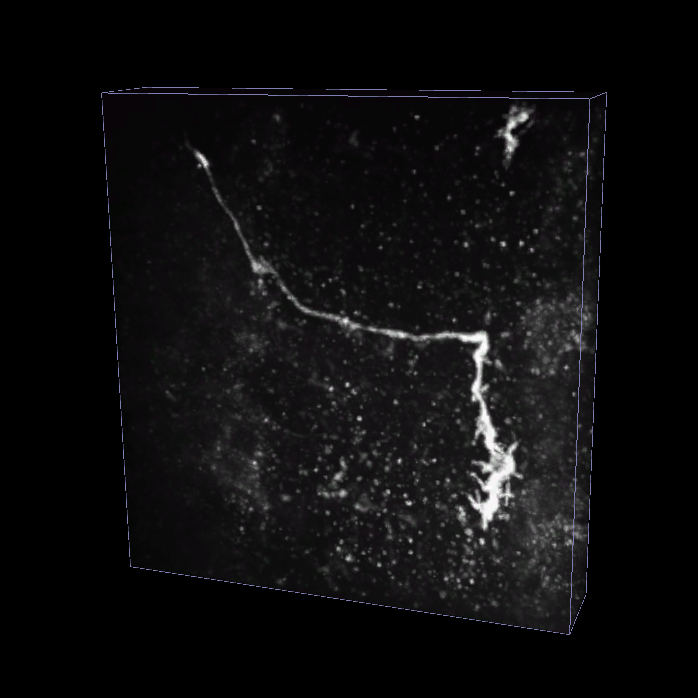
\includegraphics[width=0.29\textwidth]{images/lowSNR_1}	&
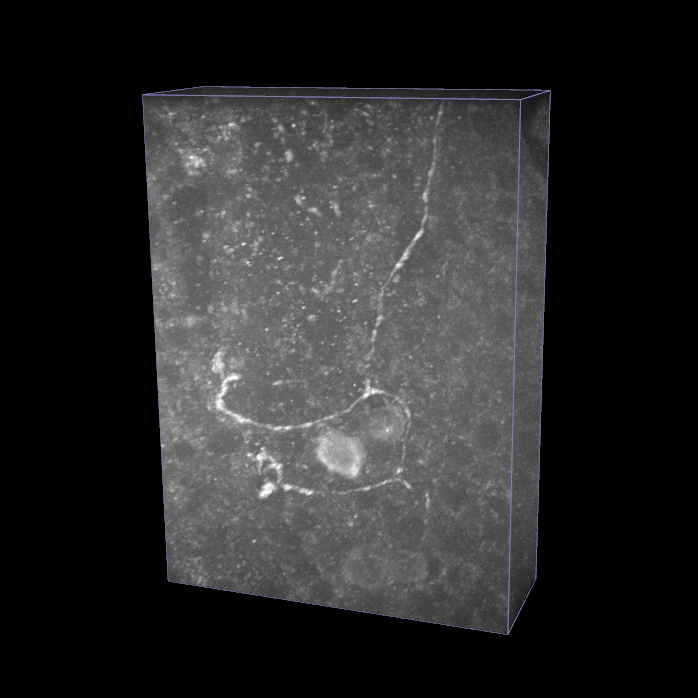
\includegraphics[width=0.29\textwidth]{images/lowSNR_2}	&
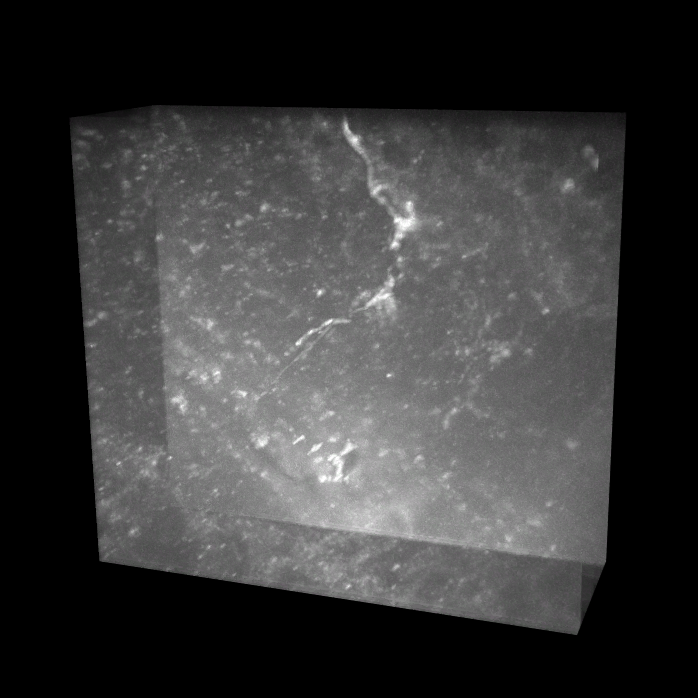
\includegraphics[width=0.29\textwidth]{images/lowSNR_3} \\
\scriptsize(a) & \scriptsize(b) & \scriptsize(c)
\end{tabular}
\caption[3D neuron example]{Drosophila neurons imaged by confocal microscope. (a) is a low SNR sensory neuron. The background clutter are due
to illuminated non neuronal filaments. (b) and (c) are interneurons, the image quality severely degraded by photon noise, low signal
intensity and in-homogeneous contrast.}
\label{fig:neuron_stack}
\end{figure}

We are interested in investigating the morphological properties of single neurons of the fruit fly Drosophila. A detailed survey of the imaging protocols is elaborate, and is out of scope of this dissertation. However, a brief summary of the imaging method is discussed here to understand on the dataset that we will be using for analyzing our algorithms.

Biologists have shown interest in studying the neuronal processes (axons, dendrites, synapses etc.) of the Drosophila, which has been a preferred model organism for to study genetics and developmental biology for several years.  The central nervous system (CNS) of the Drosophila contains a vast array of interacting synapses and neuronal processes in addition to containing about 20,000 neurons in the larval stage.  

Green Florescence Protein (GFP) is used to label the neuronal cells, which are produced through a combination of a FLP/FRT system and GAL4/UAS system. Approximately 10 hr old embryos were heat shocked at $37^\circ$C for 1-2 hrs, that generates single GFP-labeled cells \cite{barry_serotonergic}. Using this protocol, most Ventral Nerve Cord (VNC)'s have about 5 labeled cells, thus allowing for imaging of individual neurons.

For imaging the labeled cells, confocal microscopy was used to image the cells in three dimensions, with resolution in the micrometer range. Three images captured in the Condron Lab at the University of Virginia are shown in Fig.~\ref{fig:neuron_stack}





%\subsection{Neuron reconstruction posed as a vessel detection problem}
%
%As mentioned earlier, neurites are tubular structures which can be appropriately modeled as  tree shaped objects with varying degrees of branch bifurcations that determines its structural complexity. Several neuron reconstruction algorithms draw inspiration from the works in medical image analysis which focus on segmenting tubular or vascular objects from images. There have been a few methods proposed in the literature in this regard for different applications and modalities, such as segmentation of retinal blood vessels, human arteries from Computed Tomography Angiography images for detecting aneurysms \cite{gooya2012generalization,gooya2008variational,lesage2009review,shang2011vascular,nain2004vessel,jacob2004steerable,manniesing2006vessel,sofka2006retinal} etc.  Other non biomedical applications of vessel detection in the computer vision community include detection of tubular structures (such as roads, bridges etc.) from aerial images \cite{gonzalez_2010,turetken_MIP}, identifying cracks on concrete structures such as pavements and bridges \cite{oliveira2013automatic,crackd_TASE,oliveira2014crackit} etc. 
%
%However, despite the fact that the problem of vessel detection has been studied for quite some time, direct adaptation of an off-the-shelf algorithm to a particular task is still non trivial. This is due to the fact that each imaging application, with its associated modality pose different challenges in terms of denoising, object enhancement and clutter removal. For example, fluorescence microscopy images are often degraded by photon noise, inhomogeneous brightness of the objects and sporadic signal attenuation, which makes segmentation difficult. This requires an application specific approach that respects the local morphology of the structures, but is robust to the various imaging artifacts as well.  

\section{Contributions of this thesis}
The major emphasis of this dissertation will be on developing novel  algorithms for segmenting single neurons from confocal microscopy data. We realize that a large scale structural analysis of neuron groups demand efficient, automated segmentation to generate the digital morphology. Therefore, in this work, we primarily focus on developing and improving the first stepping stone for \textit{neuromics}-- automated neuron segmentation algorithms. 

%We start with a 2-d framework, and gradually progress to the more complicated 3-d segmentation problem. We identify the key issues which are necessary for robust neuron structure detection viz. prior enhancement of tubular neurites and the ability to deal with abrupt signal attenuation due to imaging artifacts. The segmentation algorithms are formulated so as to adequately respond to these issues. Finally, we propose a modification and improvement for the neuron enhancement step, which is an integral aspect for both the segmentation algorithms. We further show that the developed and proposed methodologies can also be used for a wide variety of applications which scale from bio-imaging to civil engineering. The specific aims of this dissertation are given below:
%
%\textit{The overall arrangement of the dissertation is as follows:
%
%\begin{itemize}
%\item \textbf{Chapter 1}: Introduction to the problem
%\item \textbf{Chapter 2}: Motivation and detailed background survey of segmentation of vascular structures, with an emphasis on neuron segmentation from confocal microscopy.
%\item \textbf{Chapter 3}: Motivation for using geometric active contours for seggmentation. Discussion of relevant level set based methodologies.
%\item \textbf{Chapter 4}: In this chapter we focus on neuron segmentation from 2D images and we propose a solution which tackles the inhomogeneity in the object illumination. 
%\item \textbf{Chapter 5}: In this chapter, we discuss our 3D neuron segmentation algorithm "Tubularity Flow Field (TuFF)". Qualitative and quantitative evaluation on a set of 3D confocal images  are presented. 
%\item \textbf{Chapter 6}: In this chapter, we propose a robust version of TuFF. This model incorporates a more suitable pre-processing step along with a component to reduce segmentation error due to contour leakage. A non biological application is discussed, which involves automated identification of cracks from concrete structures. 
%\item \textbf{Chapter 7}: Finally, in this chapter we conclude this thesis by discussing its salient features and identifying the future prospects. 
%\end{itemize}
%}

\subsubsection*{Contribution 1: Graph theoretic neuron segmentation}

We devise a novel neuron tracing technique Tree2Tree-2 \cite{mukherjee_T2T_2}, which combines the strengths of variational segmentation and graph based connectivity analysis of disjoint connected components. We also introduce a novel methodology to generate a \textit{medialness} function \cite{mukherjee_medialness} for tubular objects, for the purpose of obtaining a smooth tracing along the neuron centerline.

\subsubsection*{Contribution 2: Region based 2D segmentation with level sets}
2D analysis often serves as a preliminary step for understanding the anatomy of neurites. Furthermore, certain categories of neurons (e.g. sensory neurons on the cuticle layer of \textit{Drosophila} larva) are topologically flat and therefore, the third dimension of imaging does not yield useful information for analysis. In this regard, we have developed a general purpose segmentation algorithm which uses geometric active contours. The proposed algorithm, \textit{Legendre Level Set} (L2S)\cite{mukherjee_L2S} aims at segmenting the objects from microscopy images in presence of heterogeneous illumination. 

\subsubsection*{Contribution 3: Tubularity field based 3D segmentation with level sets}
We propose a novel neuron tracing architecture, Tubularity Flow Field (TuFF) \cite{mukherjee_TuFF}, which uses geometric active contours to perform segmentation guided by the local tubularity of the neurites. One advantage of using geometric active contours is that these techniques are adaptive to the topology of the objects. As a result, joining disjoint neurites can be handled in a natural framework unlike Tree2Tree-2, where error is often introduced in the solution due to improper connectivity handling. We also provide a mechanism to combat the sporadic signal loss across the structures by incorporating a specialized attraction force in our solution to merge nearby fragments. 

\section{Thesis outline}
The rest of the dissertation is organized as follows: In Chapter 2, we discuss popular neuron segmentation techniques, as well as relevant methodologies for pre-processing.  
The graph based segmentation algorithm is discussed in Chapter 3 and the results are scrutinized for both 2D and 3D data. We identify the pros and cons of our method and discuss the motivation of using geometric active contours for more flexibility in establishing component connectivity. 

In Chapter 4, a brief summary of geometric active contours is presented, followed by discussion of the proposed 2D segmentation method L2S in Chapter 5. The 3D segmentation case using TuFF is presented in Chapter 6, along with strategies to improve segmentation results using a robust non local vessel detection technique.  Finally, we conclude in Chapter 7 with discussion of the methods, their future extensions and possible applications.

Apart from the aforementioned primary contributions, we found that the developed algorithms are quite general, and have a wide variety of applications involving vascular structures. Two such applications are discussed in the Appendix; the first one involves segmenting human arteries from low SNR ultrasound imagery, and the second method relates to the civil engineering discipline, where the goal is to detect cracks in concrete structures such as bridges and pavements.

\section{Publications resulting from this work}

\textsc{Journal Publications}
\begin{itemize}
\item 
\textbf{S. Mukherjee}, B. Condron and S.T. Acton, "Tubularity Flow Field – A Technique For Automatic Neuron Segmentation," \textit{IEEE Transactions on Image Processing}, vol.24, no.1, pp.374,389, Jan. 2015

\item
\textbf{S. Mukherjee} and S.T. Acton, ``Region Based Segmentation in Presence of Intensity Inhomogeneity Using Legendre Polynomials," \textit{IEEE Signal Processing Letters}, vol.22, no.3, pp.298,302, March 2015

\item
R.Sarkar, \textbf{S. Mukherjee} and S.T. Acton, ``Dictionary Learning Level Sets" \textit{IEEE Signal Processing Letters} (\textit{under minor revision})

\item
\textbf{S. Mukherjee}, L. Boulton and S.T. Acton, "Concrete crack detection using edge assisted Tubularity Flow Field with local directional evidence", \textit{in preparation}.
\end{itemize}

\noindent \textsc{Conference Publications}
\begin{itemize}
\item
\textbf{S. Mukherjee} and S.T. Acton, ``Oriented Filters for Vessel Contrast Enhancement With Local Directional Evidence", \textit{IEEE ISBI 2015}(accepted).
\item
M. Consylman, \textbf{S. Mukherjee}, D.P. Mukherjee, B. Condron and Scott T. Acton, ``Social behavior analysis of Drosophila larvae via motion activity recognition", \textit{IEEE SSIAI 2014.}
\item
\textbf{S. Mukherjee}, B. Condron and S.T. Acton, ``Neuron segmentation with level sets", \textit{ACSSC 2013}:1078-1082
\item
R. Sarkar, \textbf{S. Mukherjee} and S. T. Acton, ``Shape descriptors based on compressed sensing with application to neuron matching", \textit{ACSSC 2013}: 970-974
\item
\textbf{S. Mukherjee} and S. T. Acton, ``Vector field convolution medialness applied to neuron tracing," \textit{ICIP 2013}: 665-669
\item
\textbf{S. Mukherjee}, B. Condron and S. T. Acton, ``Chasing the neurome: Segmentation and comparison of neurons," \textit{EUSIPCO 2013}: 1-4
\item
\textbf{S. Mukherjee}, S. Basu, B. Condron and S.T. Acton , ``Tree2Tree2: Neuron tracing in 3D," \textit{ISBI 2013}: 448-451
\item
\textbf{S. Mukherjee}, S. Basu, B. Condron and S.T. Acton, ``A geometric-statistical approach toward neuron matching", \textit{ISBI 2012}: 772-775.

\end{itemize}

%\subsubsection*{Aim 1: Algorithm for neuron segmentation in 2D}
%
%Our first goal is to develop a generalized segmentation policy for  2D microscopy images. 2D analysis often serves as a preliminary step for understanding the anatomy of neurites. Furthermore, certain categories of neurons (e.g. sensory neurons on the cuticle layer of \textit{Drosophila} larva) are topologically flat and therefore, the third dimension of imaging does not yield useful information for analysis. 
%
%In this regard, we have developed a general purpose segmentation algorithm which uses geometric active contours. The proposed algorithm, \textit{Legendre Level Set} (L2S) aims at segmenting the objects from microscopy images in presence of heterogeneous illumination. We also briefly discuss a closely related algorithm \textit{Dictionary Learning Level Set}, which uses dictionary learning to tackle the intensity inhomogeneity. 
%
%\subsubsection*{Aim 2: Algorithm for neuron segmentation in 3D}
%Morphological characteristics of a vast majority of neurons are better captured using 3D imaging. A vast majority 3D images of the Green Fluorescence Protein (GFP) stained adult \textit{Drosophila} fruit fly is obtained at the Dept. of Biology, University of Virginia using confocal microscope. The GFP is expressed in single neurons using a heat shot activated scheme, which allows imaging at the single cell resolution\cite{barry_branching}.
%
%First, we discuss a graph theoretic segmentation algorithm \textit{Tree2Tree-2}, where the idea is to treat the neuron connectivity analysis problem using graph based algorithms. Details of Tree2Tree-2 are presented in Chapter 2. The second method, \textit{Tubularity Flow Field} or TuFF uses geometric active contours to perform segmentation guided by the local tubularity of the neurites. One advantage of using geometric active contours is that these techniques are adaptive to the topology of the objects. As a result, joining disjoint neurites can be handled in a natural framework unlike Tree2Tree-2, where error is often introduced in the solution due to improper connectivity handling. We also provide a mechanism to combat the sporadic signal loss across the structures by incorporating a specialized attraction force in our solution to merge nearby fragments. 
%
%\subsubsection*{Aim 3: Robust TuFF and other applications}
%
%Tubularity Flow Field is an effective mode of segmenting vascular shapes both in 2D and 3D applications. However, there are some aspects of TuFF which limits its broad applicability. To address these needs, we discuss a robust algorithm known as \textit{Edge Assisted TuFF} or EATuFF. The major highlights of EATuFF over TuFF is the addition of a specialized preprocessing step called Local Directional Evidence (LDE) which uses non local steerable filters to identify tubular structures in low contrast imagery. Second, an edge based attraction term is associated with the TuFF segmentation framework to reduce the contour leakage phenomenon which may occur if the image contrast is low. 
%
%We further demonstrate the applicability of our algorithm for a non biological application which involves detecting cracks on concrete structures. Although the application differs significantly from microscopy, these cracks can also be modeled as tubular objects. We show that EATuFF can be efficiently applied for this application with promising results.


%% Chapter 2

\chapter{Background} % Main chapter title

\label{Chapter2} % For referencing the chapter elsewhere, use \ref{Chapter2} 

\lhead{Chapter 2. \emph{Background}} % This is for the header on each page - perhaps a shortened title

%----------------------------------------------------------------------------------------

In this chapter we present a detailed background survey of different techniques for segmenting single neurons from confocal microscopy. As we have mentioned earlier, we restrict ourselves to the case of detecting single neurons, and therefore techniques which fall under the multi neuron category, or are based on other imaging modalities (such as EM, two photon microscopy) are excluded from the discussion. 

The different neuronal components (also popularly known as neuronal processes in biology) such as dendrites and axons, imaged via confocal microscope typically exhibit filamentous appearance. A majority of the neuron image analysis algorithms exploit the filamentous nature of the structures to devise tracing methodologies in presence of background noise and clutter. Vascular or filamentous/tubular structures occur in abundance in medical imaging. This includes, but are not restricted to, retinal blood vessels, blood vessels and arteries in the brain and other organs imaged via CTA, human arteries as seen in ultrasound images etc. A majority of these images suffer from poor contrast and background noise and thereby require a preprocessing step to enhance the vascular structures before performing segmentation. 

Perhaps one of the most widely used and well known vessel enhancing method was proposed by Frangi \textit{et al} \cite{frangi_vesselness}. In the recent years, there have been significant research to develop robust algorithms to improve vessel detection from low contrast imagery. This includes 3D line filters due to Sato \textit{et al}.\cite{sato1998three}, diffusion based methods\cite{manniesing2006vessel} and steerable ridge detectors \cite{jacob2004steerable}. Vessel enhancement is an integral step in many tracing and segmentation algorithms, and will be discussed in significant detail in the next few chapters of this dissertation.


\section{Neuron segmentation and tracing}

The terms tracing and segmentation are often used interchangeably in the relevant literature. In most cases, tracing refers to the algorithms that focus on reconstruction of the neuron by identifying the centerline of the filaments. Segmentation algorithms, on the other hand are more traditional and aim at delineating the entire neuronal structure using traditional segmentation tools such as thresholding, morphological operations, connected component analysis, active contours, graph cuts etc \cite{bovik2010handbook}. The neuron tracing can be obtained from the segmented result by computing the centerline of the binary segments using skeletonization algorithms \cite{bovik2010handbook}.  However, before we discuss the algorithms for neuron tracing, let us briefly talk about the biological motivation and imaging technique for data acquisition.

\subsection{Challenges in image processing}

Confocal microscopy is a popular method for imaging single neuron cells. The ability to visualize neurons at a single cell resolution is a significant step towards automated structure identification.  Confocal laser scanning microscopes (CLSM) use focused laser beams to excite selectively tagged neurons (which are labeled with a florescent protein) to emit energy in form of photons, which are subsequently absorbed by a photodetector to create an image of the objects at the particular optical plane. Out of plane scatter is suppressed by the detector aperture, thus allowing sharper image formation.  Information can be collected  from different focal planes by altering the focal length of the system, thus creating multiple slices (z-stacks), which are eventually fused to form a 3D image of the specimen. 


Like many other light microscopy techniques, neuron imaging using confocal microscopy comes with its own set of challenges. First, most images are low contrast and suffer from low signal to noise ratio. Photobleaching effect restricts the imaging time, which directly affects the signal intensity and contrast. Also, irregular photon emission from the filaments, especially those at greater depths, creates inhomogeneous signal intensity and renders a fragmented appearance of the neurites. Finally, the images are affected by photon noise and clutter resulting from non neuronal fluorescing tissues. All these aspects make image processing challenging and a suitable neuron tracer needs to manage these artifacts using sophisticated image processing.  Fig.~\ref{fig:neuron_stack_demo} shows an example of the imaging artifacts discussed here.
\begin{figure}[t]
\centering
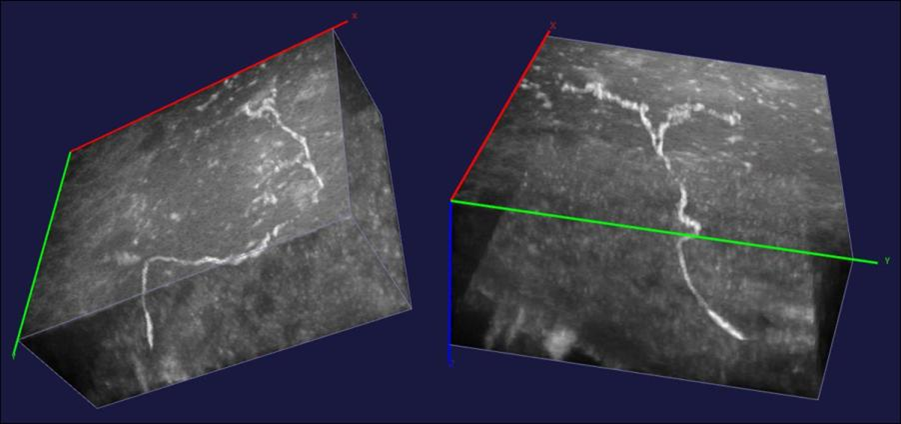
\includegraphics[width=0.8\textwidth]{images/3D_demo}	
\caption[Imaging artifacts]{A 3D confocal microscopy image of Drosophila interneuron is shown from two viewing angles. The image is degraded by low contrast and inhomogeneous illumination of the neurite. Furthermore, presence of noise and background clutter deteriorates the image quality.}
\label{fig:neuron_stack_demo}
\end{figure}

\subsection{Neuron tracing strategies}
In this section we are going to highlight some popular neuron tracing and segmentation works. Most of these tools are extensively used by biologists for segmentation of single neurons. However, the list is  definitely not exhaustive and more algorithms are being developed each day as the field continues to grow.

We can broadly categorize the neuron segmentation schemes in two basic approaches. The first set of methods use user defined (or automatically detected) initial seed points to perform tracing in a local exploratory manner. Such methods are popularly known as \textit{tracing} algorithms or \textit{tracers}, since the algorithms locally trace the neuron centerlines. The second category of algorithms avoid seed initialization and perform segmentation using a combination of local and global features. In the next few subsections, we will discuss a few popular neuron tracing and segmentation algorithms. 

\subsubsection{NeuronJ}
One of the earlier works in neuron tracing was proposed by Meijering \textit{et al.}\cite{meijering2004design}. The tracing algorithm, NeuronJ, is a 2D neuron tracer, which uses specialized steerable ridge detector kernels \cite{jacob2004steerable} to determine the evidence of a neuron filament, which the authors call \textit{neuriteness}. A semi automated graph based tracing method \textit{Livewire} \cite{livewire} is then used to trace the neurite centerline, using evidence of neuriteness from the ridge detector response. 

NeuronJ is widely used in the scientific community for 2D tracing, and it owes its popularity to its robustness and simplicity, and is available as a plugin for the open source, bio-imaging software ImageJ\cite{imageJ}. However, the method is custom made for 2D imagery only, and carrying out such user interactive tracing in 3D appears less trivial. Also, the algorithm relies significantly on user assistance, especially for determining branch points and neurite terminals. As a result, the applicability of this tool is somewhat limited for high throughput analysis.
 
\subsubsection{Simple Neurite Tracer}
Simple Neurite Tracer\cite{SNT} is another open source, publicly available, semi-automated 3D neuron tracer.
Simple Neurite Tracer (SNT) falls under the category of seed-based tracing algorithm, where the user selects a set of initial points on the neuron centerline. A graph is then created, with these seed points serving as the nodes of the graph, and the edge weights depending on their relative distance and the vessel intensity at the seed locations. A shortest path algorithm\cite{dijkstra1959note} is then deployed to compute the best possible path between the adjacent seeds. 

Like many vessel tracing algorithms, SNT also uses vessel enhancement technique \cite{frangi_vesselness,sato1998three} for determining the shortest path between the seeds. Similar to NeuronJ, SNT is also available as a plugin for ImageJ. However, the major drawback of SNT include the excessive use of human assistance (for seed detection, merge point identification etc.) for tracing. That being said, SNT is popular among biologists and is often used as a post processing platform for correcting or editing neuron reconstructions from automated tracers.

\subsubsection{Vaa3D and associated algorithms}
Vaa3D\cite{peng_v3d} is a neuron tracing software suit which is gaining significant popularity in the recent years. The C++ based tracing suit hosts a number of neuron tracing algorithms, both seed based and automated. One popular method, Graph Augmented Deformable model (GD model) was proposed by Peng \textit{et al}\cite{peng_GAD}. The GD model performs neuron tracing based on some user chosen seeds, which are typically chosen as the neurite terminals. With these set of chosen locations, tracing is performed between the pairwise seeds using a deformable, shortest path approach. Fast and accurate segmentation is possible using the above mentioned approaches if the neuron morphology is simple and the image noise level is low. Recent algorithms proposed by the same group \cite{peng_anisotropicPS,peng_APP} attempts to make the tracing more user independent by initially performing an over segmentation by choosing a conservative threshold, followed by pruning to delete unwanted components. 

\subsubsection{k-Minimum Spanning Tree}
Gonzalez \textit{et al}. \cite{turetken_Diadem} introduced a graph theoretic technique to delineate the optimal neuronal tree from an initial set of seeds by computing a k-Minimum Spanning Tree. To automatically generate the seed points, the authors propose using a supervised learning methodology to determine potential neurite locations. This neuron probability map is importance sampled to generate a set of seeds, with special care taken to preserve the important locations such as tips and bifurcations. 

Since the minimum spanning tree of a graph created from all the nodes can contain non neuronal clutter, the authors propose a novel solution by posing am optimization problem that finds the k\textsuperscript{th} minimum spanning tree. An approximate solution to this NP-hard problem is realized by minimizing a global energy function in a linear integer programming framework. Recently, there have been efforts to improve the accuracy of the algorithm, by using a different optimization criteria\cite{turetken_MIP}. 

\subsubsection{NeuronStudio}
NeuronStudio\cite{wearne_neuronStudio} is a neuron segmentation software toolkit. Unlike the aforementioned methods, which are essentiially tracing techniques and rely on initial seed selection, NeuronStudio is an example of a traditional segmentation algorithm. The algorithm implemented is known as \textit{voxel scooping} method\cite{rodriguez_voxelscoop}. It assumes that the neurites are locally tubular filaments and iteratively searches for voxel clusters in a manner similar to region growing. A pruning step is then deployed to eliminate spurious end nodes.

The biggest aspect of NeuronStudio is that it is relatively less dependent on user interaction, and segmentation only requires a single seed location to identify the starting position for region growing. However, the region growing algorithm becomes less stable when the images are degraded by low contrast, and region leakage becomes an issue for processing.

\subsubsection{Open-Curve Snake}
The Open-Curve Snake method\cite{wang_Roysam_open_curve,cai_ISBI} is implemented using open ended parametric active contours. This can be considered to be a tracing method, where the 1D curves are evolved along the vessel centerline to perform tracing. An external force field is suitably designed for curve evolution, which encourages the trace to lie along the neuron centerline. A preprocessing step based on tensor voting \cite{roysam_tensorvoting} is also used to enhance the neuron contrast and the snake initialization is performed by using graph cuts\cite{graph_cut} to get an initial overestimate of the neurite locations. Combined with a post-processing step to eliminate false filaments, this method is efficient in segmenting neuronal structures from low SNR confocal stacks. However, due to the inability of parametric active contours to naturally handle topological changes such as object merging, neurite branch point detection depends requires a non-trivial post processing to determine snake merging at the junctions.
 
\subsubsection{Tree2Tree}
Tree2Tree \cite{basu_T2T_journal} aims to solve the neuron segmentation problem in a graph theoretic framework. Unlike traditional seed selection approaches, where manually designated points are treated as the nodes of the graph, an initial segmentation algorithm is devised to produce a set of disjoint binary connected components. Connectivity between the components is analyzed based on their separating distance and orientation, which determines the weights of the graph edges to perform segmentation using a minimum spanning tree approach. 

Although the primary contribution of Tree2Tree is to connect the fragmented neurite segments automatically, this connectivity analysis relies on heavily on the initialization. Noise and clutter in the images create undesired artifacts in the global segmentation, resulting in loss of structural information. Moreover, linking the components based on their relative geometric orientation requires computation of the leaf-tangents from the object centerlines, which is sensitive to the irregularities of the neurite surface. One drawback of Tree2Tree is that the disjoint neighboring neurite fragments are connected by a splined curve, which may not coincide with the actual neurite location in the image. This aspect of Tree2Tree is addressed in Tree2Tree2\cite{mukherjee_T2T_2}, which will be discussed in more details in Chapter  \ref{T2T2_chapter}.

\subsubsection{Other methods}
Apart from the above mentioned algorithms which are popular in the scientific community since the implementation is readily available, there are many more tracing methodologies that deserve mention. Al-Kofahi \textit{et al}. \cite{al_kofahi} used the medial response of multiple directional templates to determine the  direction to generate successive seed points along the neuron medial axis. This local tracing method shows good performance in high-contrast images, but requires continuity in the neuron branches for reliable segmentation. Other notable neuron tracers include the wavelet based algorithm due to \cite{dima_wavalet}, morphology and graph theory based technique of Chothani\textit{et al.} \cite{chothani2011automated} etc. 

Other methods of segmentation include the use of probabilistic region merging\cite{srinivasan2007automated},  tracking based algorithms \cite{wang2007dynamic,choromanska2012automatic} and active contours \cite{wang2011novel}. A survey of recent tools for neuron reconstruction is available due to Dr. Erik Meijering\cite{meijering_survey}.

The medical imaging community has performed substantial research in developing algorithms to detect and segment filamentous shapes in non-microscopy medical images \cite{lesage2009review}. While not related directly to neuron tracing or segmentation, methods for segmenting vasculature have been extended or modified for tracing neurons, and thereby deserve mention.

The CURVES algorithm by Lorigo \textit{et al}. \cite{lorigo2001curves} evolves a 1D curve along a 3D vessel centerline guided by the curvature of a 1D curve. Gooya \textit{et al}.\cite{gooya2008variational} developed an elegant and generalizable  regularization methodology to enhance the performance of the popular geometric curve evolution methods. The method allows for anisotropic curve propagation  which minimizes contour leakage when vessel edge information is weak. One apparent downside of this technique is that the ultimate solution somewhat depends on the shape of the initialized contour. Another recent work by Gooya \textit{et al}.\cite{gooya2012generalization} generalizes the flux maximizing flow \cite{flux_max} on Riemann manifolds and uses a vessel enhancing tensor, which improves segmentation when edge detection is less accurate.

Shang \textit{et al}. \cite{shang2011vascular} developed a vessel tracing algorithm where wider vessels are first segmented using a region based criteria. Then the eigenvectors of the hessian matrix are utilized to derive a geometric flow equation to segment the thinner vessels. Santamaria-Pang \textit{et al}. \cite{santamaria2007automatic} use a multistage procedure for detection of tubular structures in multi-photon imagery, which includes a pre-filtering stage to identify the filaments based on supervised learning. However, this requires offline learning of the model parameters and prior knowledge about the vessel appearance information, which necessitates a set of accurate training examples and demands extensive human involvement to generate the ground truth.

\section{Discussion}
The neuron segmentation algorithms discussed in this chapter are classified either as local tracers, or global segmentation techniques. We hypothesize that seed based local algorithms are useful if the imaged neurons are not too complicated structurally. In such scenarios, where manual seed selection is easy, reliable segmentation can be obtained. However, since automatically choosing the correct set of seed points is still an open problem, it is difficult to use the above mentioned techniques for high throughput, no intervention analysis. Also, since proper selection of seeds points is instrumental in these methods, the segmentation accuracy is sometimes compromised if a sub-optimal set of points is chosen. Furthermore, the connectivity analysis between the seeds assume uniform signal intensity, and noise and low contrast in the images may degrade the segmentation quality.

In contrast to the seed based local techniques, traditional segmentation approaches are more global, typically requiring an initial pre-processing of the image followed by a specialized segmentation step. Although a global approach may suffer from expensive computation, they are more suitable for neurite junction and end point detection.
Typically, such methods rely on a four stage processing pipeline -- enhancement, segmentation, centerline detection and post processing. However, despite being less dependent on user interaction, global segmentation algorithms should be adequately modeled to capture the finer details of neurite geometry, such as complex branching patterns, including twists and turns of filaments and should be capable of handling signal attenuation due to imaging artifacts.

Due to the aforementioned reasons, we refrain from using local seed based techniques for segmenting neurons. In the following chapters, three novel neuron segmentation methods are presented, which are completely automated and do not require manual identification of seed points for tracing.  
%\chapter{Graph Based Neuron Tracing} % Main chapter title

\label{T2T2_chapter} % For referencing the chapter elsewhere, use \ref{Chapter2} 

\lhead{Chapter 3. \emph{Tree2Tree-2}} % This is for the header on each page - perhaps a shortened title

In this chapter we will discuss our first neuron tracing algorithm, which uses graph theoretic algorithms to perform tracing. The proposed algorithm, Tree2Tree-2\cite{mukherjee_T2T_2} extends the former neuron tracer Tree2Tree, which was proposed by Basu \textit{et al.}\cite{basu_T2T_journal}. Both Tree2Tree and Tree2Tree-2 are hybrid algorithms in a sense that they combine strategies of both segmentation based techniques and graph based tracing. The idea is to start with an initial set of neurite segments, which are possibly disjoint, and then identify the connectivity between them. In the next few sections, we will discuss the properties of Tree2Tree-2 in more detail.

\section{Tree2Tree-2}
The general workflow of Tree2Tree-2  consists of three major steps: image denoising and filament enhancement, initial segmentatation and connectivity analysis .
\begin{figure}[t]
\centering
\begin{tabular}{c}
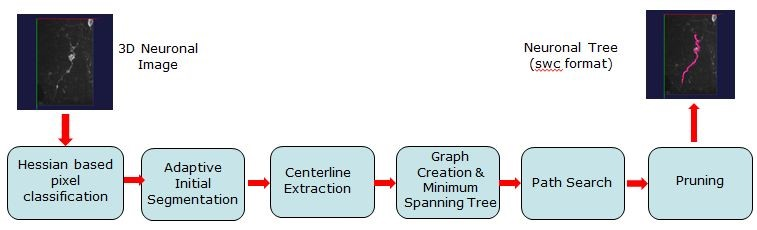
\includegraphics[width=0.8\linewidth]{./images/ch3/T2T2_pipeline.jpg}	
\end{tabular}
\caption[Tree2Tree-2: workflow]{The working pipeline of Tree2Tree-2}
\label{fig:T2T2_pipeline}
\end{figure}


\subsection{Hessian based vessel enhancement}
Frangi's \cite{frangi_vesselness} method for enhancing vascular structures is based on analyzing the geometric features of tubular objects. The vesselness or tubularity measure at a point $\textbf{x}\in \Omega$ in the image $f:\Omega \rightarrow \mathbb{R}$ can be obtained by examining the hessian matrix of the gaussian smoothed image over a set of scales. The hessian of the $d$-dimensional image $f(\textbf{x})$ at a position \textbf{x} and scale $\sigma$ is the square matrix $\mathcal{H}_{\sigma}(\textbf{x})=\left[ h \right]_{i,j} $ ($1\leq{i,j}\leq{d}, \; \textbf{x}\in\Omega$) which is given by
\bea
	 h_{i,j}=\frac{\partial^2G(\sigma)}{\partial x_i \partial x_j}*f(\textbf{x})
\eea 
Here \textbf{x} is the $d$-dimensional vector $\textbf{x}=\left(x_1,\ldots, x_d \right)^T$, $G(\sigma)$ is the zero mean normalized Gaussian kernel with variance $\sigma^2$. Here $d=2 $ or 3 for 2-D or 3-D images respectively.

At any position $\textbf{x}$ on the image surface, the local curvature in the direction of the vector $\textbf{v}$ is given by $\textbf{v}^T\mathcal{H}_\sigma(\textbf{x})\textbf{v}$. If $\textbf{v}$ is the direction along the vessel centerline (or major axis if we approximate a vessel locally as a cylinder), we expect the curvature to be negligible, assuming that the vessel intensity is homogeneous. On the other hand, in the directions orthogonal to the vessel axis, we encounter significantly higher curvature. Therefore, based on these curvature values, one can develop a discriminatory function (\textit{vesselness}) to differentiate between vascular and non vascular objects.

\subsubsection{Tubularity field}
From the above discussion, at a position $\textbf{x}\in \Omega$, a 3-D tubular structure can be characterized by three principal directions:
(i) an axial direction along which the second derivative is negligible, and (ii) two orthogonal directions along which the second derivative magnitude is significant. These directions are given by the orthonormal set of eigenvectors $\{\textbf{e}_1\left(\textbf{x}\right),\textbf{e}_2\left(\textbf{x}\right),\textbf{e}_3\left(\textbf{x}\right)\}$ of the hessian matrix(see Fig.~\ref{fig:frangi_vessel}(a)). The corresponding second derivative magnitudes or the curvature values are obtained from the respective eigenvalues as follows: $|\lambda_1(\textbf{x})|\leq{|\lambda_2(\textbf{x})|\leq{|\lambda_3(\textbf{x})|}}$.
\begin{figure}[t]
\centering
\begin{tabular}{ccc}
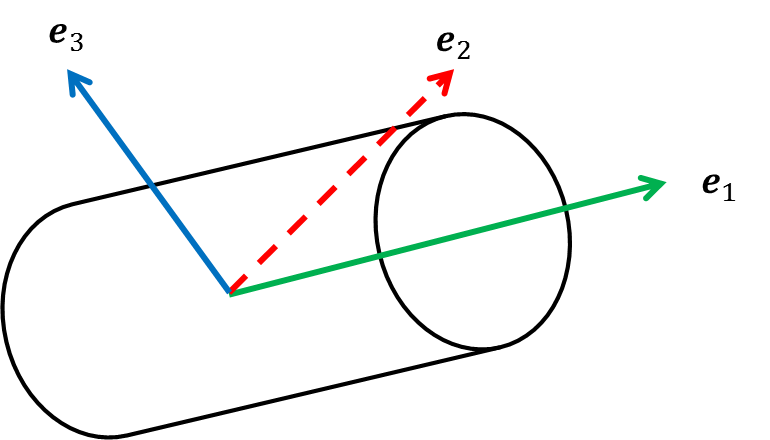
\includegraphics[width=0.3\textwidth]{images/ch2/3dvessel}	&
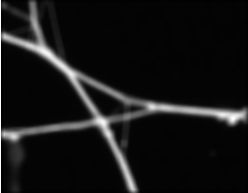
\includegraphics[width=0.25\textwidth]{images/ch2/vessel}	&
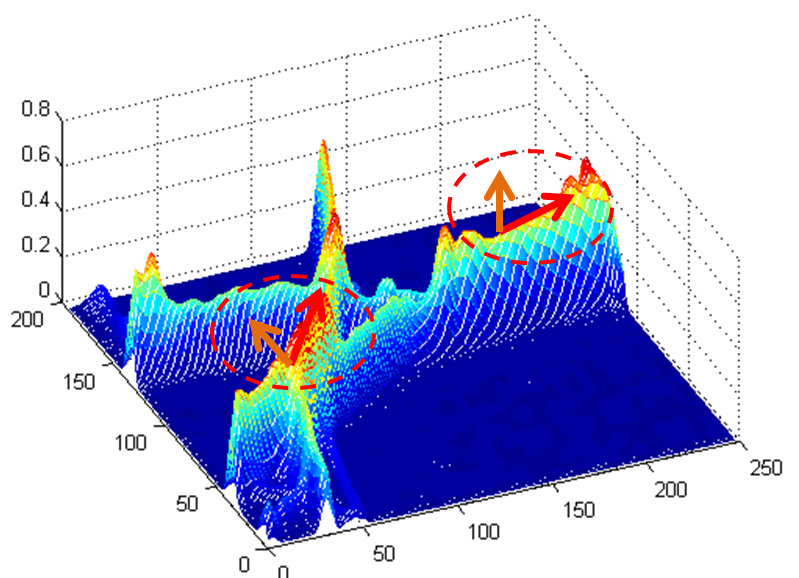
\includegraphics[width=0.3\textwidth]{images/ch2/vessel_mesh} \\
\scriptsize(a) & \scriptsize(b) & \scriptsize(c) \\
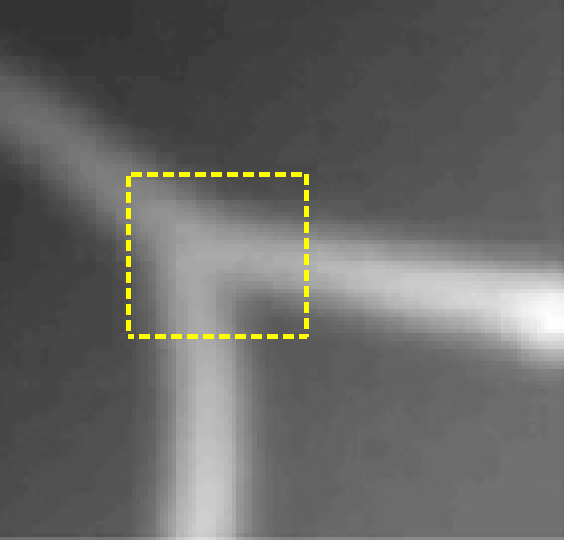
\includegraphics[width=0.28\textwidth]{images/ch2/orig}	&
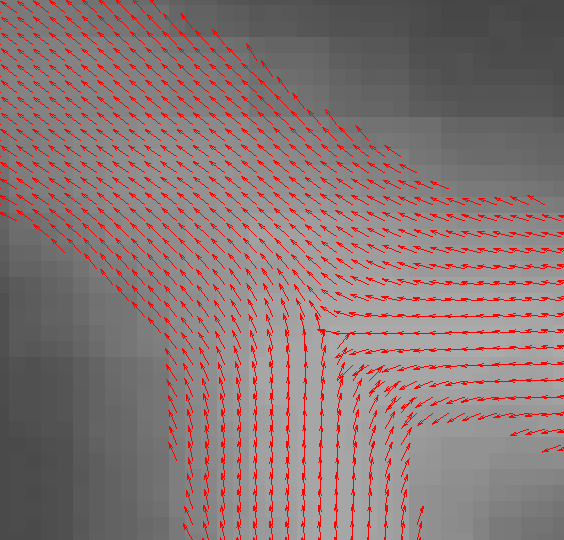
\includegraphics[width=0.28\textwidth]{images/ch2/F1}	&
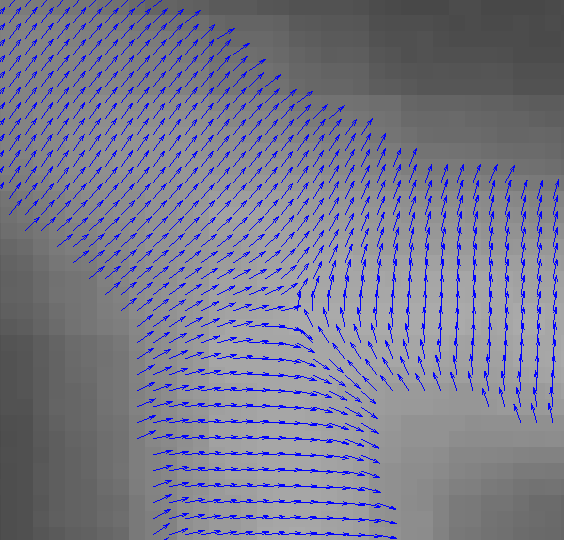
\includegraphics[width=0.28\textwidth]{images/ch2/F2} \\
\scriptsize(d) & \scriptsize(e) & \scriptsize(f) \\
\end{tabular}
\caption[Tubularity field]{(a) Graphic demonstration of the tubularity fields. (b) An image of a neurite and (c) corresponding surface plot of the image. Vessel orientations are shown by the red and orange vectors. This figure is best viewed in color. (d) A real example of a vascular structure. (e) Axial field $\textbf{e}_1$ and (f) Normal field $\textbf{e}_2$ for the zoomed portion.}
\label{fig:frangi_vessel}
\end{figure}
It may be observed that for a filamentous voxel \textbf{x}, the eigenvalues of its hessian matrix (computed at scale $\sigma$) should satisfy the following criteria:
\begin{gather}
\label{eq:3d_hessian}
|\lambda_1(\textbf{x})|\approx 0 \nn\\
|\lambda_2(\textbf{x})|\gg|\lambda_1(\textbf{x})|,\;|\lambda_3(\textbf{x})|\gg|\lambda_1(\textbf{x})| \\
|\lambda_2(\textbf{x})|\approx|\lambda_3(\textbf{x})|  \nn
\end{gather}
Also, assuming that vascular filaments are brighter than the background, we have  $\lambda_2(\textbf{x})<0$ and $\lambda_3(\textbf{x})<0$. A voxel that belongs to a vessel should satisfy the above mentioned criteria. Based on that, there has been several vessel enhancement measures proposed in the literature \cite{frangi_vesselness,basu_T2T_journal}.  For example, Basu \textit{et al}. \cite{basu_T2T_journal} suggests the following vesselness function $N_\sigma$ at scale $\sigma$  for enhancing the tubular structures:
\bea
	N_{\sigma}(\textbf{x})=
	\begin{cases}
		\dfrac{|\lambda_1(\textbf{x})-\lambda_2(\textbf{x})|^2}{|\lambda_1(\textbf{x})||\lambda_2(\textbf{x})-\lambda_3(\textbf{x})|} & \text{if $\lambda_2(\textbf{x}),\lambda_3(\textbf{x})< 0$} \\
		0 & \text{otherwise}
	\end{cases}
\eea
Also, since the filament thickness can vary, a multiscale analysis is essential. This can be evaluated by computing the maxima across a set of predefined scales, known as the scale space $S=\{\sigma_{min},\ldots,\sigma_{max}\}$.
\bea
	\sigma^*(\textbf{x})=\arg\!\max_{\sigma \in S}N_{\sigma}(\textbf{x}) \label{eq:optimal_scale}\\
	N(\textbf{x})=\max_{\sigma \in S}N_{\sigma}(\textbf{x}) \label{eq:vesselness_scale}
\eea
The scale space vesselness function $N(\textbf{x})$  assumes higher value at locations of local tubularity over non-filamentous positions. It should be noted that (\ref{eq:vesselness_scale}) yields evidence of the presence of vasculature by suppressing the non-filamentous structures, thus introducing a mechanism for dealing with noise and non tubular clutter.

\subsection{Initial Segmentation}

\begin{figure}[thb]
\centering
\begin{tabular}{ccc}
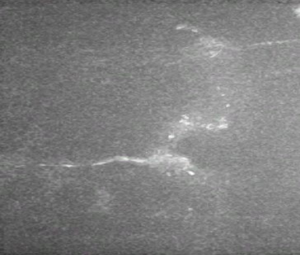
\includegraphics[width=0.3\linewidth, height = 0.25\linewidth]{./images/ch3/raw_demo}	&
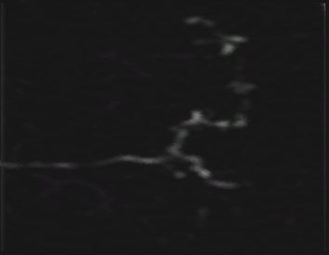
\includegraphics[width=0.3\linewidth, height = 0.25\linewidth]{./images/ch3/hessian_demo}	&
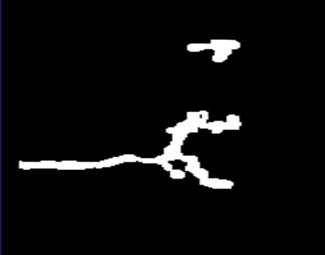
\includegraphics[width=0.3\linewidth, height = 0.25\linewidth]{./images/ch3/binary_demo}	\\
\scriptsize (a) & \scriptsize (b) & \scriptsize (c)
\end{tabular}
\caption[Tree2Tree-2: Initial segmentation]{Illustration of the enhancement and initial segmentation stage of Tree2Tree-2. (a) 3-D confocal image, (b) hessian enhanced image $N(\textbf{x})$ and (c) binary image, showing the two disjoint connected components after thresholding.}
\label{fig:T2T_enhance}
\end{figure}
Once the raw confocal image is denoised and the vessel contrast improved using the aforementioned technique, the obtained vesselness function (\ref{eq:vesselness_scale}) is segmented to get an initial estimate of neurite locations. The major aspect of Tree2Tree-2 is to integrate the possibly disjoint components obtained in the segmentation step. Since the connectivity analysis step is non-generative, we choose a local segmentation technique using variational minimax\cite{saha_minimax} to get a possibly overestimated solution having multiple binary connected components. The mathematical formulation of our segmentation framework is presented here.

Let $f:\Omega\mapsto\mathbb{R}$ be an image, and $N$ denotes the vesselness function which is computed using (\ref{eq:vesselness_scale}). We define a threshold surface $s(\textbf{x})$, $\textbf{x}\in\Omega$ such that our initial  segmentation result is given by the binary image $b:\Omega\mapsto \{0,1\} $ which is defined as follows:
\bea
	b(\textbf{x})=
	\begin{cases}
		1 & \text{if $N(\textbf{x})>s(\textbf{x})$} \\
		0 & \text{otherwise}
	\end{cases}
	\label{eq:minimax_binary}
\eea
The optimal threshold surface is computed by minimizing a convex energy functional $E(s,\alpha)$
\bea
E(s,\alpha) =\displaystyle \dfrac{1}{2}\sqrt{1-\alpha^2}\underbrace{\int_{\Omega}\left(N-s\right)^2|\nabla N|^2 d\textbf{x}}_{E_1} + \dfrac{1}{2}\alpha\underbrace{\int_{\Omega}|\nabla s|^2 d\textbf{x}}_{E_2}
\label{eq:minimax_func}
\eea
The first term in (\ref{eq:minimax_func}), $E_1$ is the data term, which computes the weighted mean square distance between the threshold function  the vesselness function. The second term, $E_2$ is a smoothness enforcing term that restricts the threshold function to develop high gradients. The relative contribution of these two functionals is controlled by the  parameter $\alpha$.

The gradient of the vesselness map corresponds to the filament edges. Therefore, the data term of the energy functional is significantly high at the filament edges, and the threshold function $s(\textbf{x})$ should be close to $N(\textbf{x})$ at edge position to reduce the cost functional in (\ref{eq:minimax_func}).

We seek to minimize (\ref{eq:minimax_func})  and since $E(s,\alpha)$ is convex with respect to $s(\textbf{x})$, the minimizing function $s^*$ is a global minima. Also, further analysis of (\ref{eq:minimax_func}) suggests that the functional is concave with respect to the scalar parameter $\alpha$. It may be observed that the characteristics of $E_1$ and $E_2$ are conflicting in a sense that the minimizer of $E_1$ does not entirely satisfy $E_2$, and vice-versa. One solution to this parameter selection problem is to use minimax technique. In a minimax paradigm, the optimal threshold surface is the one which minimizes the worst case cost function. Mathematically, this is stated as:
\bea
\{s^*(\textbf{x}),\alpha^*\} = \text{arg}\max_\alpha\min_s E(s(\textbf{x}),\alpha)
\label{eq:minimax_formulate}
\eea
We solve (\ref{eq:minimax_formulate}) using variational calculus for $s$, and the  obtained Euler-Lagrange equation is solved using gradient descent. We use alternating maximization to compute  $\alpha$. The solution is derived as follows. Please refer to the Appendix \ref{AppendixTuFF} for details of derivation.
\bea
\dfrac{\partial s}{\partial t} &=& \sqrt{1-(\alpha^*)^2}|\nabla N|^2\left(N-s\right)+\alpha^*\nabla^2 s\nn \\
\alpha^* &=&\dfrac{E_2}{\sqrt{E_1^2+E_2^2}}
\label{eq:minimax_soln}
\eea
We solve (\ref{eq:minimax_soln}) via discrete approximation of the partial differential equation, with Neumann boundary conditions. The optimal threshold  surface  is obtained at convergence, and then the initial segmentation $b(\textbf{x})$ is derived using (\ref{eq:minimax_binary}). The initial segmentation gives us an estimate of the neuron morphology. However, the imaged neurons may appear fragmented due to imaging artifacts. This can create multiple segments, instead of getting a single connected component (see Fig. ~\ref{fig:T2T_enhance}(c)), some of which may not belong to the original neuron. Therefore, to establish the global neural morphology, we introduce a method to analyze the connectivity between the different fragments, followed by a specialized pruning step to discard clutter.

\subsection{Connectivity analysis and component linking}
\begin{figure}[bht]
\centering
\begin{tabular}{cc}
\includegraphics[width=0.62\linewidth]{./images/graph_connectivity_a}	&
\includegraphics[width=0.3\linewidth]{./images/graph_connectivity_b}	\\
\scriptsize (a) & \scriptsize (b) 
\end{tabular}
\caption[T2T2: establishing global graph]{(a) The calculation of orientation and distance between leaf pairs. 2 synthetic connected components $C_i$ and $C_j$ shown in blue. 6 pairs of leaf node connectivity (shown in dotted green) are tested for the closest distance between the components. The closest leaf pair is indicated. (b)Two disjoint components are joined by the global connectivity algorithm (shown in red). However, the actual path is unknown and is decided by PathSearch.}
\label{fig:T2T2_conn}
\end{figure}
The primary contribution of Tree2Tree-2 is to analyze and determine proper connectivity between the disjoint segments (see Fig.~\ref{fig:T2T2_conn}). We adopt a graph theoretic approach to determine possible connections between the branches. Once this is established, the next step would be to physically link the components by a curve which traces the medial axis of the neurite filaments. 

The initial segmentation procedure classifies the image voxels into neuronal (foreground) and non-neuronal (background) portions, as shown in Fig.~\ref{fig:T2T_enhance}(c). Since the obtained foreground segments may be disjoint, the next step is to connect the components to obtain a global graph, and eventually, the neuronal tree. To ensure proper connectivity, we adopt a two stage procedure.

Let us denote the set of disjoint components as  $C=\{C_1,\ldots,C_n\}$.  The first step involves a global graph connectivity algorithm that decides  the connectivity between these components. The edge weights of the complete graph, created with the set of nodes $\{C\}$ are computed such that more probable connections have lower weights. Basu \textit{et al}.\cite{basu_T2T_journal} designed the edge weight function such that the weight $D_{ij}$ is low when two components $C_i$ and $C_j$ are close according to the euclidean distance metric and they are oriented towards each other. Mathematically, this is can be stated in the following manner: 
\bea
D_{ij} = \lambda \textit{dist}(C_i,C_j) + (1-\lambda)\textit{orientation}(C_i,C_j)
\label{eq:T2T2_globalgraph}
\eea
Here $dist()$ is a function that computes the shortest euclidean distance between the terminals of $C_i$ and $C_j$. The function $orientation()$ assumes a high value if the outward leaf tangent vectors of the connected components are facing in the same direction. An illustrative example is shown in Fig.~\ref{fig:T2T2_conn}(a). For detailed description, we refer the reader to the original paper \cite{basu_T2T_journal}.

A Minimum Spanning Tree (MST) of the global graph produces an initial neuronal tree. This method is computationally simple and provides efficient and accurate connectivity information between the components. The objective now is to detect the actual path that connects them in the image domain.

We devise a novel algorithm, PathSearch, which finds the  physical connection (in the image domain) between the components which are deemed suitable for joining in the initial graph based analysis step. 

\subsection{PathSearch}

The PathSearch algorithm to find the physical path between the terminal points of two disjoint components uses Dijkstra's method \cite{dijkstra1959note} to find the shortest path between the end points. Treating each voxel as a node in a graph, the edge weight between two neighboring voxels $\textbf{x}$ and $\textbf{y}$ is computed as
\bea
w(\textbf{x},\textbf{y})=\frac{2}{\mu(\textbf{x})+\mu(\textbf{y})}
\label{eq:pathsearch}
\eea
Non-neighbors are not connected by an edge. Here, we assume 26-connectivity of the voxels in 3D (8-connectivity in 2D). $\mu(\textbf{x}),\mu(\textbf{y})$ denote the medialness value at voxel positions $\textbf{x}$ and $\textbf{y}$, which assumes a higher value at voxels near the medial axis than those away from the medial axis\cite{mukherjee_medialness}\footnote{For implementation, only a subset of pixels in a window containing the two endpoints are considered, to make processing faster.}. Choice of this weight function ensures that two voxels on a neuron medial axis are connected by a lower edge weight than two arbitrary, non-neuronal voxels. With this edge weight defined on the graph, we now use Dijkstra's shortest path algorithm \cite{dijkstra1959note} to determine the path connecting the end points between two segments. To get a smooth connection, we further interpolate this path by fitting a cubic B-spline to this curve. The workflow of the PathSearch method can be summarized as follows:
\begin{enumerate}
\item Determine the  connectivity between the end nodes of the disjoint binary components using relative orientation and euclidean distance between the components.
\item Compute the neuron tree using MST.
\item Compute a medialness map to produce evidence of a path along neuron medial axis (cf. \cite{mukherjee_medialness}).
\item Join the end points (in the image domain) by computing the shortest path between them using suitable edge weight function.
\item Smooth the obtained trace by spline fitting.
\end{enumerate}

\section{Multiscale medialness map}

In the previous section, we mentioned that the PathSearch algorithm joins the components via shortest path along the medial axis of the underlying neuron. This requires computing a \textit{medialness} function $\mu(\textbf{x})$ (see (\ref{eq:pathsearch})), which assumes higher values at the object medial axis. 

Finding medial axis for binary structures is a well studied problem in mathematical morphology\cite{bovik2010handbook}. However, the problem is non trivial for gray scale objects. In this section, we introduce a technique for computing a medialness map for non binary objects and we use the computed medialness value for neuron tracing via Tree2Tree-2. 

\subsection{Vector field convolution medialness}
\begin{figure}[thb]
\centering
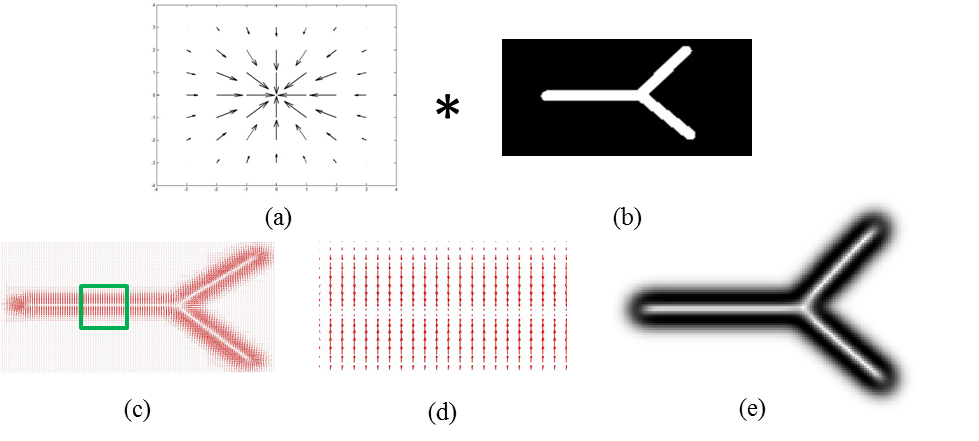
\includegraphics[width=1\linewidth]{./images/VFC/medialness}	
\caption[VFC medialness]{A discrete VFC kernel is shown in (a). (b) shows a synthetic tubular structure. (c) illustrates the vector fields after convolving (b) with the kernel, at some scale. An enhanced view is shown in (d), which reveals that the vectors cancel at the medial axis. The computed scale-space medialness map is shown in (c).}
\label{fig:medialness}
\end{figure}
\noindent We propose a novel method to compute the medialness function of a grayscale object using vector field convolution (VFC) [11], which is computationally efficient and robust to noise. The vector field convolution kernel is defined as
\bea
K_{\gamma}(\textbf{x})=m_\gamma(\textbf{x})\frac{\textbf{x}}{||\textbf{x}||}
\label{eq:VFC_ker}
\eea
The kernel is designed such the the vectors are directed towards the kernel center $\textbf{x}=0$. Magnitude of the vectors is determined by the magnitude function $m_\gamma(\textbf{x})$. Choosing $m_\gamma(\textbf{p})=\exp(-||\textbf{p}||^{2}/\gamma^{2})$, we create a kernel such that the influence of the vector field diminishes away from the center. This \emph{kernel range} can be tuned by the scale parameter $\gamma$. A sample VFC kernel is shown for illustration in Fig.~\ref{fig:medialness}(a). At the correct scale, convolution of an image with the VFC kernel produces a zero magnitude vector at the points of symmetry of the grayscale object, since the vectors cancel each other. The points of symmetry of an object can be recognized by finding the local minima in the convolved image (assuming the object is brighter than the background). Mathematically, at a scale $\gamma$, the vector field obtained after convolving the image $f(\textbf{x})$ with the kernel in (\ref{eq:VFC_ker}) is given as $V_{\gamma}(\textbf{x})= f(\textbf{x})*K_{\gamma}(\textbf{x})$. At this particular scale, the medialness is defined as
\bea
\mu_{\gamma}(\textbf{x})=1-\frac{|V_{\gamma}(\textbf{x})|-\min|V_{\gamma}|}{\max|V_{\gamma}|-\min|V_{\gamma}|}
\label{eq:med_scale}
\eea

\subsection{Multiscale VFC medialness}
Since the neurite thickness varies, a multiscale approach is required to obtain a scale invariant medialness function.  Let $\Theta$ be the scale space, which captures thickness of the objects of interest. In order to evaluate the correct medialness response over the scale space, we observe that the medialness response of a non-medial point diminishes with increasing scale, whereas, the response is significant for the medial points for each scale. The scale space medialness map is computed as
\bea
\mu(\textbf{x})=\frac{1}{|\Theta|}\sum_{\gamma \in \Theta}\mu_{\gamma}(\textbf{x})
\label{eq:medialness_map}
\eea
Fig.~\ref{fig:medialness} illustrates the medial map computation on a synthetic tubular object. Fig.~\ref{fig:medialness}(c) shows the vector field, which is generated by convolving the image (b) with the VFC kernel (at a fixed scale). The scale space medialness map is shown in Fig.~\ref{fig:medialness}(e). 


\section{Computing the neuronal tree}
To summarize Tree2Tree-2, we first compute a global neuron tree using MST, where the connectivity information between the terminals of the neurite fragments are derived based on the relative geometry of the components. Then, PathSearch is used to physically connect the endpoints, by finding the shortest path between the terminals, which adheres to the medial axis of the neurite filaments.
Let us designate the global tree obtained using MST and PathSearch as $\Gamma=\{E,V,W\}$. Here $E = \{e\},V=\{v_{ij}\}$ and $W=\{w_{ij}\}$ denote the sets of edges, nodes and edge weights of the global tree.
The  nodes $v\in V$ correspond to the individual segments obtained after initial segmentation, and the edges $e_{ij}\in E$ between the nodes $(v_i,v_j)$  are computed via PathSearch. To assign the weight $w(e_{ij})\in W$ to an edge $e_{ij}$, we compute the sum of the edge weights of the shortest path between $v_i$ and $v_j$. This ensures that false edges have a higher path weight than the true connections. 

However, since the initial segmentation step may result in over segmentation, we may eventually get undesired nodes in the neuron tree due to the presence of clutter. 
This leads to the final step of Tree2Tree-2, where a pruning methodology is deployed to eliminate the false nodes.
\subsection{Tree pruning}
\begin{figure}[t]
\centering
\begin{tabular}{cc}
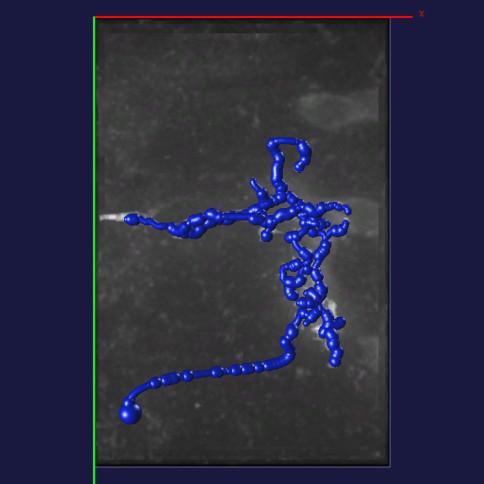
\includegraphics[width=0.4\textwidth]{images/ch3/clutter1}	&
\includegraphics[width=0.4\textwidth]{images/ch3/clutter1_pruned}	\\
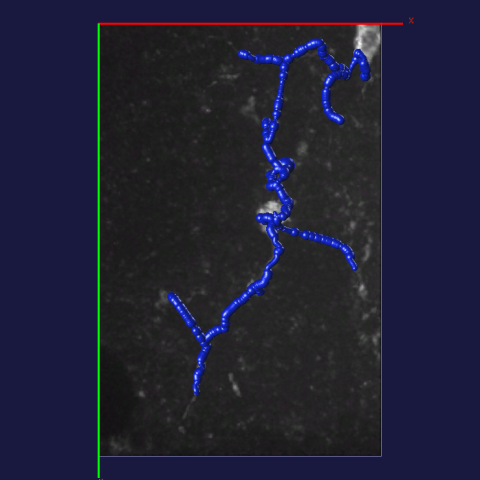
\includegraphics[width=0.4\textwidth]{images/ch3/clutter2}	&
\includegraphics[width=0.4\textwidth]{images/ch3/clutter2_pruned}	\\
\scriptsize(a) & \scriptsize(b)
\end{tabular}
\caption[Tree2Tree-2 graph pruning]{Results of graph pruning. (a) A global neuron tree using MST+PathSearch. (b) The pruned tree with the false nodes removed.}
\label{fig:T2T2_pruning}
\end{figure}
We designate the volume (area) occupied by a tree in the 3D (2D) binary image as $\psi(\Gamma)$. Our assumption is that the neuronal portions occupy more volume than the clutter, and the cost of connecting them via PathSearch is more compared to a true node. We devise the following method to prune the tree: 

Let $e\in E$ be an edge in the tree, i.e.$w(e)\geq w(e'),\, \forall e\in E$. Removing this edge from the tree $\Gamma$ creates two disjoint subtrees $\Gamma_1$ and $\Gamma_2$. Let us denote $\Gamma^* = \underset{\Gamma_j}{\arg\min}\,\psi(\Gamma_j)$. From standard graph theory, the graph $\Gamma\setminus\Gamma^*$ that results from removing the subtree $\Gamma^*$ from the global tree $\Gamma$, is also a subtree. 

Our strategy for pruning the tree is as follows. We select a scalar variable $\rho \in \left[0,1\right]$, which may be defined by the user.  The subtree $\Gamma^*$ is removed from the tree if $\dfrac{\psi(\Gamma^*)}{\psi(\Gamma)}\leq \rho$. The pruning process is repeated till no subtree can be further removed from the tree. Using this strategy, a subtree is deleted if it is connected by a significantly high cost path (which signifies higher possibility of a false connection), and the volume occupied by the subtree is small enough compared to the overall volume (since the area/volume of the clutter is significantly lower than the neurites). Typically, we use a low value of $\rho$$ (\approx 0.1)$, which  encourages removal of clutter over a neuron segment (Fig.~\ref{fig:T2T2_pruning}).
\begin{figure}[tb]
\centering
\begin{tabular}{cc}
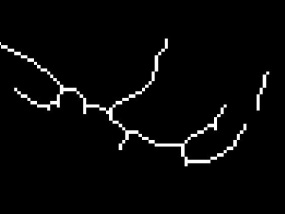
\includegraphics[width=0.4\textwidth]{images/ch3/broken}	&
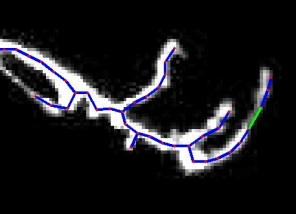
\includegraphics[height=0.302\textwidth]{images/ch3/connected}	\\
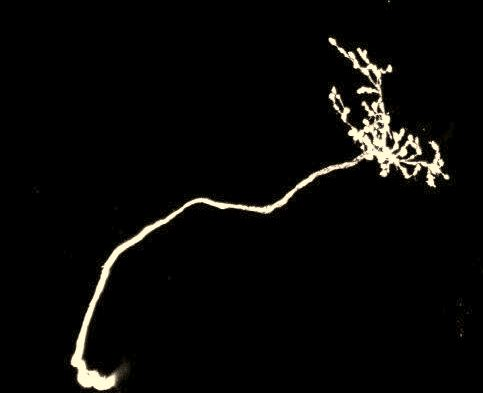
\includegraphics[width=0.4\textwidth]{images/ch3/n4}	&
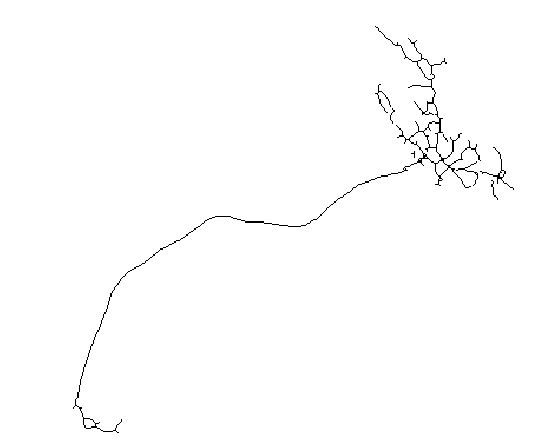
\includegraphics[width=0.4\textwidth]{images/ch3/n4_VFC}	\\
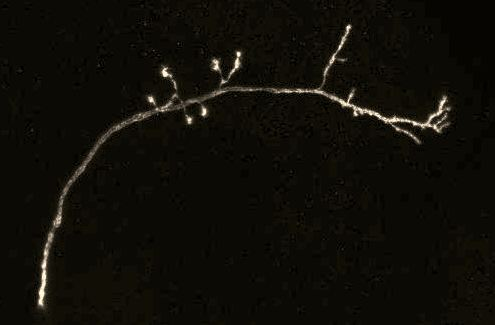
\includegraphics[width=0.4\textwidth]{images/ch3/n7}	&
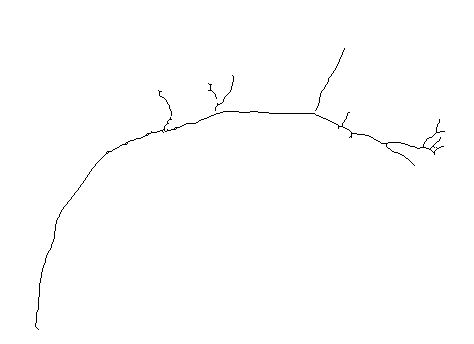
\includegraphics[width=0.4\textwidth]{images/ch3/n7_VFC}	
\end{tabular}
\caption[Tree2Tree-2: 2D results]{The top row shows an example how a broken link is joined by Tree2Tree-2 in 2D. The resulting tracing is shown in the second column and the detected connectivity is shown in green. Rows 2 and 3 show Tree2Tree-2 tracing results on 2D maximum intensity projection neuron images. The traced results are shown in the second column.}
\label{fig:T2T2_results2D}
\end{figure}

\section{Results}
Tree2Tree-2 is a tracing algorithm, applicable to both 2D and 3D images. We first present a few qualitative tracing results on 2D images. The 2D images are obtained using maximum intensity projection of the 3D stacks along the Z-axis (depth). Fig.~\ref{fig:T2T2_results2D} shows the tracing results of Tree2Tree-2 on a few 2D images. 
\begin{figure}[t]
\centering
\begin{tabular}{cc}
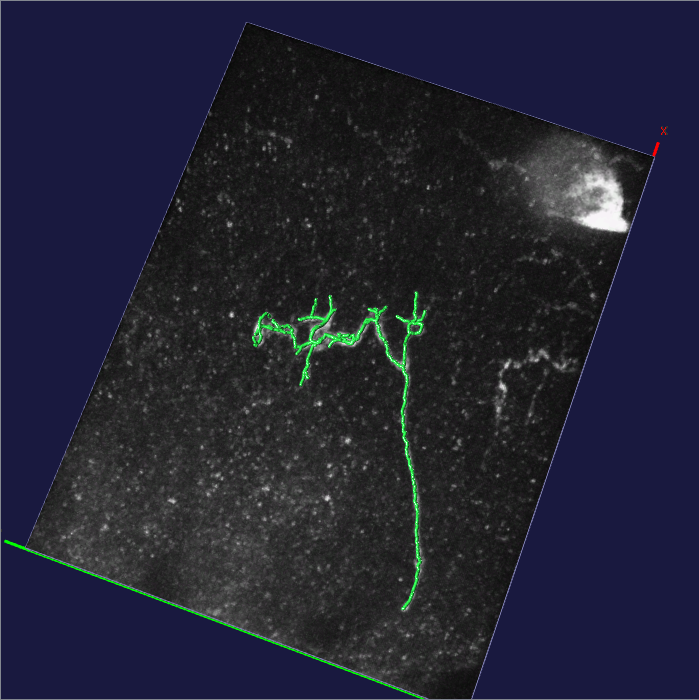
\includegraphics[width=0.4\textwidth]{images/ch3/T2T2_3D1_org}	&
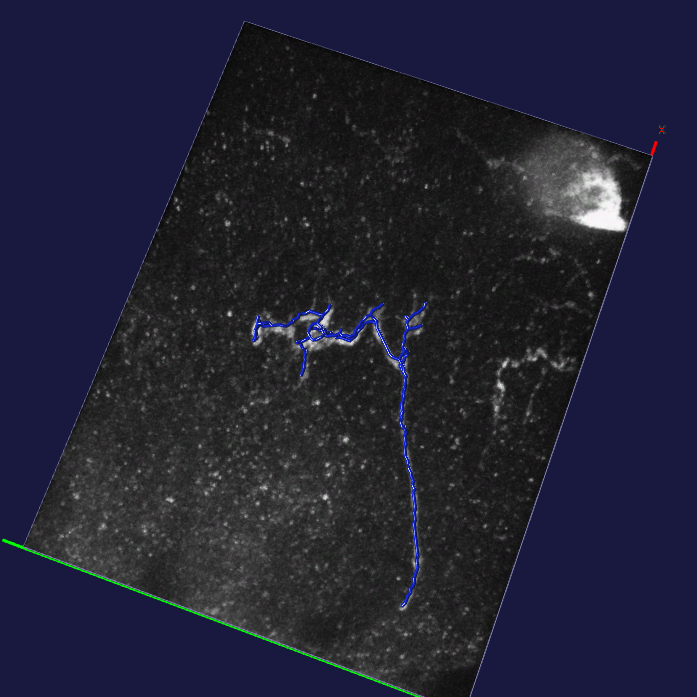
\includegraphics[height=0.4\textwidth]{images/ch3/T2T2_3D1}	\\
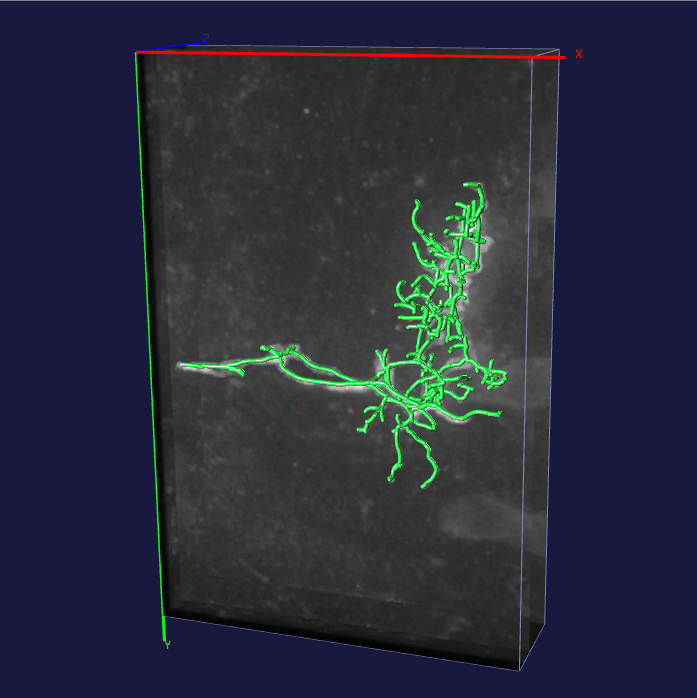
\includegraphics[width=0.4\textwidth]{images/ch3/T2T2_3D2_org}	&
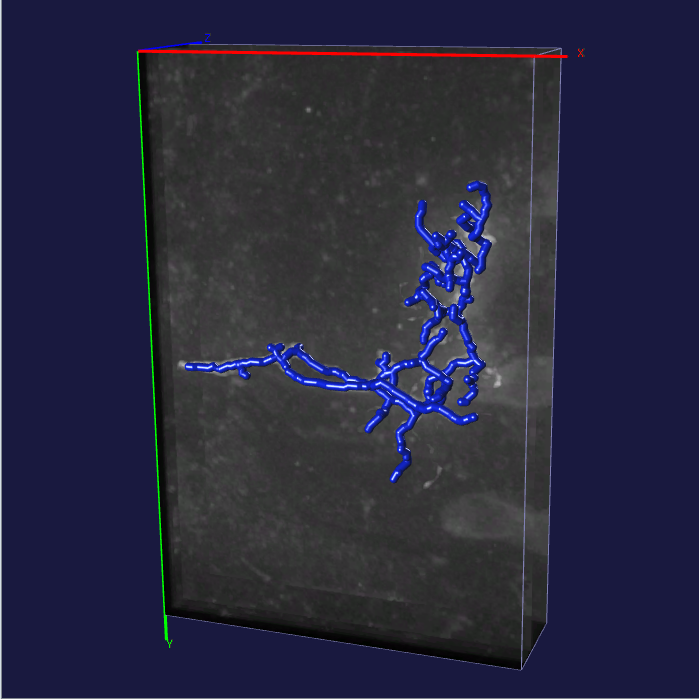
\includegraphics[width=0.4\textwidth]{images/ch3/T2T2_3D2}	\\
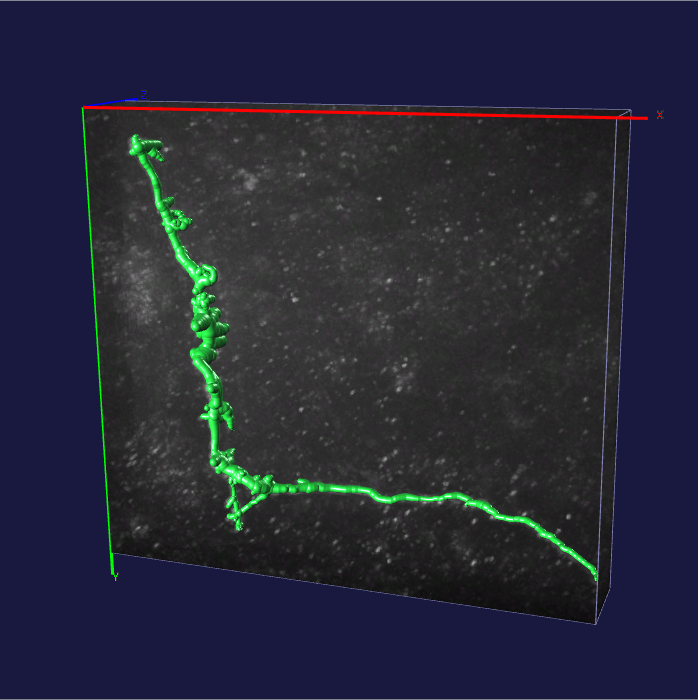
\includegraphics[width=0.4\textwidth]{images/ch3/T2T2_3D3_orig}	&
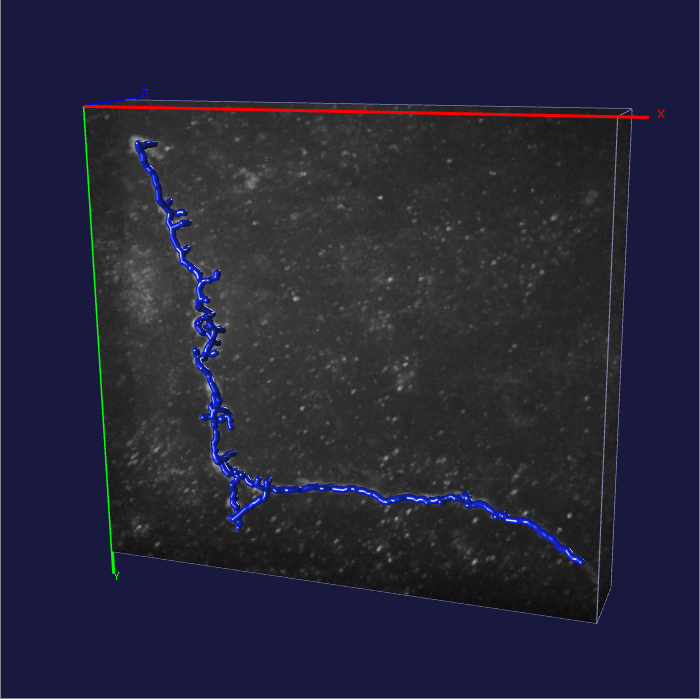
\includegraphics[width=0.4\textwidth]{images/ch3/T2T2_3D3}	
\end{tabular}
\caption[Tree2Tree-2: 3D results]{The first column shows manual tracing results(green). 3D tracing results of Tree2Tree-2 are shown in the second column (blue). The splined centerline is plotted on the original 3D confocal images of the Drosophila larva.}
\label{fig:T2T2_results3D}
\end{figure}
Qualitative results for 3D tracing are shown in Fig.~\ref{fig:T2T2_results3D}. The manual tracing results are shown in the first column, and are overlaid on the original images using the Vaa3D visualization software\cite{peng_v3d}. Tracing results due to Tree2Tree-2 are shown in the second column in blue. 

To quantify the performance of Tree2Tree-2, we use the normalized Mean Absolute Error (NMAE)\cite{basu_T2T_journal} of the traced neuron, with respect to the manually annotated tracings. Preliminary experiments were performed on a batch of ten 3D stacks, which contained noisy images of Drosophila neurites. We observed an average NMAE of 1.01\%, as compared to 1.97\% for that of its precursor algorithm Tree2Tree \cite{basu_T2T_journal}. The improvement in performance is largely due to the fact that Tree2Tree-2 uses PathSearch to compute the physical path between two objects, where Tree2Tree uses splines to interpolate the positions between two fragments. Also, the proposed tree pruning method in Tree2Tree-2 is simpler and more efficient compared to the alpha-beta pruning step in Tree2Tree.
\clearpage
\section{Discussion}
The proposed algorithm, Tree2Tree-2 is essentially a neuron tracing method which leverages the capabilities of graph theoretic algorithms to identify the centerlines of the neuron filaments. The primary contribution of Tree2Tree-2 is to determine the connectivity between the different binary objects, which are obtained via initial segmentation of the neurites. From that perspective, Tree2Tree-2 can be considered an intelligent component analysis algorithm. Using simple graph based methods, we are  able to compute the centerlines of neurites with considerable accuracy, given that the structural complexity is not significant. The initial segmentation step requires few parameters, and therefore helps automating the process. Moreover, Tree2Tree-2 revisits the component connectivity issue from the image domain perspective as well, once the initial connectivity information is obtained using graphs. This allows us to accurately connect the neurites along physical paths, as opposed to interpolating them in Tree2Tree. Also, since efficient algorithms exist to compute  MST and shortest paths, Tree2Tree-2 is computationally efficient.

However, on the downside, Tree2Tree-2 relies on the initial segmentation step. If components are lost during thresholding, the algorithm is unable to interpolate the neurite structure. Therefore, it is preferable that the initial segmentation overestimates the solution. 

However, such under segmentation can result in multiple binary components, which reduces the efficacy of the graph based connectivity analysis portion of Tree2Tree-2. In fact, since the neurite connections are analyzed only between the end points of the objects, it does not accommodate all possible cases of discontinuities. As a result, structural complexity of the filaments, as well as the number of binary objects in the solution degrades the tracing performance by predicting false edges between the fragments. Two examples are shown in Fig.~\ref{fig:T2T2_error}. In Fig.~\ref{fig:T2T2_error}(a), we demonstrate a 2D example, where the initial segmentation resulted in the tracing in blue. The green lines show the links predicted by Tree2Tree-2. The region highlighted by the red circle shows a situation, where the component connectivity cannot be resolved by analyzing the end points of the fragments. However, since Tree2Tree-2 cannot handle discontinuities which are not between the object termini, a false branch is predicted. A similar result is shown in (b) for a 3D image, where Tree2Tree-2 forces the objects to be connected between the two terminals. 
\begin{figure}[th]
\centering
\begin{tabular}{cc}
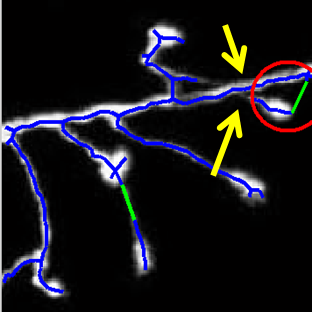
\includegraphics[width=0.45\textwidth]{images/ch3/error1}	&
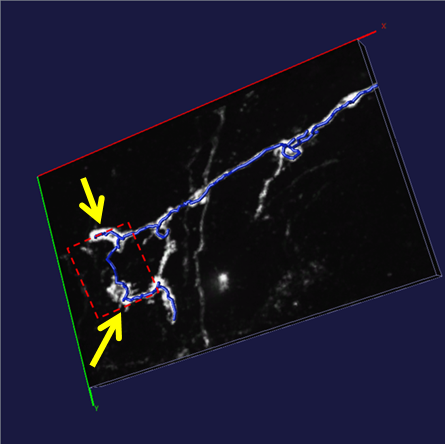
\includegraphics[height=0.45\textwidth]{images/ch3/error2} \\
\scriptsize (a) & \scriptsize (b)
\end{tabular}
\caption[Tree2Tree-2: connectivity errors]{Examples of false edge prediction by Tree2Tree-2. In both examples, error in connectivity results from Tree2Tree-2's inability to handle discontinuities which are not between the end points of the objects. Improper branch connections are highlighted  by yellow arrows. Regions enclosed by the red curves show the regions of interests. }
\label{fig:T2T2_error}
\end{figure}
While such a branch can be removed by pruning the tree, it would result in the removal of a subtree, which  contains a real neurite portion. Therefore, investing in  a pruning strategy is not the most effective way to solve this problem. We hypothesize that such connectivity related issues can be better handled if the segmentation methodology is naturally able to adapt to the object topology. For example, so far we have been interested in determining the appropriate connections between the objects; however, a segmentation method which does not require such explicit connectivity analysis would fare better in circumstances where the neuron structures are complicated. This motivates us to use geometric deformable models \cite{osher_sethian,caselles_geodesic} for segmenting complicated structures like neurons. In such a paradigm the object topology is handled automatically, and if the model is appropriately designed, there is no need to assess the connectivity information based on geometrical position of the objects. In the next chapter, we present a  brief overview of geometric active contours and surfaces for segmentation, and we formalize a procedure to use them for our application in the following chapters.

























%% Chapter 3

\chapter{Geometric Active Contours} % Main chapter title

\label{GAC_chapter} % For referencing the chapter elsewhere, use \ref{Chapter2} 

\lhead{Chapter 4. \emph{Geometric Active Contours}} % This is for the header on each page - perhaps a shortened title

%----------------------------------------------------------------------------------------

Object detection and image segmentation are arguably one of the more investigated fields in computer vision and image analysis. Although in certain cases the terms detection and segmentation are used almost synonymously, there exists subtle differences between them; an object detection algorithm can be deemed successful if it can effectively determine and localize the object of interest in the image. Segmentation, however, requires finer analysis. In segmentation problems, one is more concerned with the morphological properties of the object such as shape, connectivity etc. and therefore, a crude detection is not always sufficient. One may think of object detection as the first step for segmentation. In fact, many segmentation methods allow the user to perform an initial detection, either automatically or semi-automatically. The segmentation algorithm then starts from the initialized position and eventually converges when the object boundaries are captured.

Active contour based methods (a.k.a. \textit{snakes}) fall under the category of segmentation algorithms which assume the image to be a  continuous and possibly differentiable function. The basic reason for such continuous domain modeling is that the mathematical formulation can be done with the help of continuous domain calculus, which is remarkably strong and well established. The continuous model is eventually discretized, using tools from numerical analysis for practical implementation.

\section{Framework for contour propagation}

Let $f(\textbf{x}):\Omega\mapsto\mathbb{R}$ be a continuous image function, $\forall\textbf{x}\in\Omega$. Traditionally, the domain $\Omega\subseteq\mathbb{R}^2$ or  $\Omega\subset\mathbb{R}^3$ for 2D or 3D cases respectively. In the 3D case, we have \textit{active surfaces} instead of active contours and the formulations are modified accordingly. However, most of the mathematics and models are consistent between 2D and 3D applications and therefore, for the sake of simplicity, we will restrict ourselves to the 2D case for basic analysis in this chapter. In the next chapter, where we introduce an explicit 3D model, we will discuss the theories for the 3D case separately. Also, we will only discuss closed curves in this chapter. Implementing open ended curves in a geometric framework is nontrivial and demands separate and elaborate treatment.

Considering we have a 2D image $f(\textbf{x}),\;\textbf{x}=(x,y)\in\Omega\subseteq\mathbb{R}^2$, we define a parametric curve $\textbf{C}(p)=\{\textbf{x}(p)\}$\footnote{$\textbf{C}_t = \dfrac{\partial \textbf{C}}{\partial t}$, where $t$ is the parameter denoting pseudo time.}, where the parameter $p\in\left[0,1\right]$. To perform segmentation, an initial contour is deformed under the influence of a force field. Mathematically, one can write the curve evolution equation as $\textbf{C}_t(p)=\textbf{F}$. Here $\textbf{F}$ is the \textit{curve velocity}, which is also known as \textit{force vector}. Decomposing the velocity in the normal and tangential direction, we derive the general curve evolution equation as follows:
\bea
\textbf{C}_t(p) = F_n(p)\textbf{n}(p)+F_t(p)\textbf{t}(p)
\label{eq:curve_evolve_n&t}
\eea
Here $\textbf{n}(p)$ and $\textbf{t}(p)$ are the unit outward normal and the tangent vectors to the curve respectively at $\textbf{x}(p)$. For the sake of brevity, we will drop the implied parameter $p$ from  future equations. The above equation defines a model for the propagation of the curve. The speed terms $F_n$ and $F_t$ contribute to the curve motion in the normal and tangential directions respectively. Since the tangential component does not explicitly contribute to the motion, but only results in a re-parametrization of the curve, (\ref{eq:curve_evolve_n&t}) may be modified as follows:
\bea
\textbf{C}_t = F\textbf{n}
\label{eq:curve_evolve_general}
\eea
The major engineering issue is to come up with a proper \textit{speed function} or \textit{evolution force} term $F$. In fact, active contour based segmentation methods are primarily concerned with the development of a problem specific, suitable evolution force term. Before we go into the analysis and implementation details, let us discuss a few popular motion models for snakes.

\section{Motion models for snakes} 

In this section, we will review some popular snake motion models. We will discuss the different choices of  the force function and their effect on the curve motion.
\subsection{Constant speed evolution}
This is the most basic active contour model, where the speed function is a constant scalar. The motion model can be stated as follows:
\bea
\textbf{C}_t = c_0\;\textbf{n}
\label{eq:const_speed}
\eea
Here, the speed function is a constant scalar $c_0$ everywhere and the curve moves in the direction of the normal (or in the opposite direction if $c_0<0$) with a constant speed. One physical example of such a motion model is that of wave front propagation according to Huygen's principle. Depending whether $c_0$ is positive or negative, such a motion model either inflates or deflates the curve. 

\subsection{Curvature based motion}
In (\ref{eq:const_speed}), each point on the snake would move with the same speed. The curvature based motion gives higher priority to the snake regions with high curvature. This inhibits the snake to develop an irregular shape during evolution. If $\kappa(p)$ be the curvature of $\textbf{C}(p)$ at positions $\textbf{x}(p)$, the curvature based motion model is stated as follows:
\bea
\textbf{C}_t = \kappa\;\textbf{n}
\label{eq:curvature_motion}
\eea
The curvature can be computed as $\kappa=-\text{div}\left(\textbf{n}\right)$. The curvature based motion model has nice geometric interpretations. It can be shown that the 2D version of mean curvature motion results in minimizing the total euclidean length of the contour \cite{grayson1987heat}. As a result, this model is often used in conjunction with other motion models for regularizing the shape of the active contour. An illustrative example is shown in Fig.~\ref{fig:mean_curvature_demo}.
\begin{figure}[t]
\centering
\begin{tabular}{cccc}
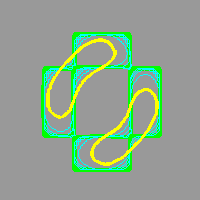
\includegraphics[width=0.22\textwidth]{images/demo/curvature_flow/curvature_flow5}	&
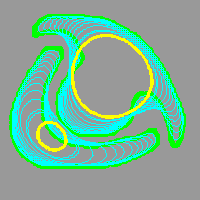
\includegraphics[width=0.22\textwidth]{images/demo/curvature_flow/curvature_flow6}	&
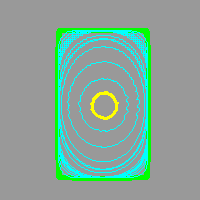
\includegraphics[width=0.22\textwidth]{images/demo/curvature_flow/curvature_flow7}	&
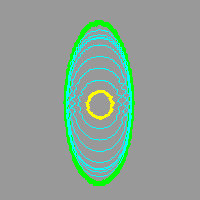
\includegraphics[width=0.22\textwidth]{images/demo/curvature_flow/curvature_flow8}
\end{tabular}
\caption[Motion by mean curvature.]{Example of motion by mean curvature. Initial curve is shown in green and the result after 500 iterations is shown in yellow. Intermediate stages of curve evolution are shown in cyan.}
\label{fig:mean_curvature_demo}
\end{figure}
For 3D applications, we have a closed surface instead of a curve. An area minimizing regularizer can be obtained by replacing the curvature term $\kappa$ in 2D by $H$ which is the sum of the principal curvatures of the surface in 3D \cite{caselles_minimal_surface}. However, unlike the 2D case, mean curvature motion is not the optimal area minimizing flow and there has been other models proposed in the literature \cite{caselles_minimal_surface,tannenbaum1997invariant}.

\subsection{Malladi-Sethian model}
The  above mentioned motion models are not really suitable for object segmentation, since neither (\ref{eq:const_speed}) or (\ref{eq:curvature_motion}) consider any information from the image. Malladi and Sethian \cite{malladi_sethian} introduced a flow based on the image model for object segmentation based on the gradient of the image. If $g(|\nabla f|)$ is a function which assumes a high value at the homogeneous portions of the image and significantly low value($\approx 0$) at the edges. One particular realization may be computed as $g=1/(1+|\nabla f|^q)$. With this definition, the curve motion equation is realized as:
\bea
\textbf{C}_t = g(|\nabla f|)(c_0+\kappa)\;\textbf{n}
\label{eq:malladi_sethian}
\eea
The function $g(.)$ acts as an edge indicator, by slowing down the speed of the snake when it approaches an edge, characterized by high gradient value. As before, the sign of the scalar $c_0$ dictates whether the snake moves outward or inward. The curvature based term imparts smoothness to the solution by disallowing irregular contour shapes.


\subsection{Geodesic Active Contour (GAC)}
\begin{figure}[t]
\centering
\renewcommand{\tabcolsep}{0.05cm}
\begin{tabular}{@{}ccc@{}}

\includegraphics[width=0.3\textwidth]{images/demo/GAC/blobs_gaussian}	&
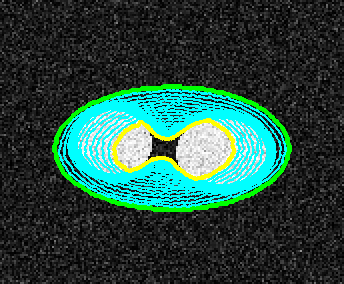
\includegraphics[width=0.3\textwidth]{images/demo/GAC/malladi_bad}	&
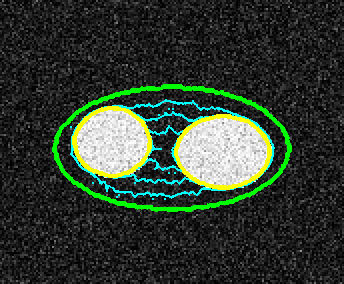
\includegraphics[width=0.3\textwidth]{images/demo/GAC/GAC_good}	\\
(a) original image & (b) Malladi-Sethian  & (c) GAC
\end{tabular}
\caption[GAC vs Malladi-Sethian model]{Segmentation performance of geodesic active contour model over Malladi-Sethian's method. The initial curve is shown in green and the final contour in yellow. Intermediate steps are shown in cyan.}
\label{fig:GACvsMalladi}
\end{figure}
Caselles et al.\cite{caselles_GAC} realized a drawback of Malladi's model which restricted its applicability in certain scenarios. This is because the function $g(.)$ does not stop the snake propagation at the edges, but merely slows it down. Therefore, if the gradient magnitude at the edges are not significantly high, the propagating curve may not converge at the boundary but continues its motion and eventually either collapses or diverges. To mitigate this issue, the geodesic active contour model was proposed, which is mathematically expressed as:
\bea
\textbf{C}_t = g(|\nabla f|)(c_0+\kappa)\;\textbf{n}-\langle\nabla g,\textbf{n} \rangle \;\textbf{n}
\label{eq:GAC}
\eea
The first part of (\ref{eq:GAC}) is similar to that of Malladi's model. The second term improves segmentation by incorporating a speed term which attracts the evolving curve towards the edge. This results in an additional component which halts the snake at the object boundaries. This is particularly helpful, since the function $g(.)$ does not stop the curve from leaking across the edges; it merely slows down the propagation speed. With the additional attraction term, the moving contour is attracted toward the edges and forces the curve to stop moving (see Fig.~\ref{fig:GACvsMalladi}).

 
This model can be interpreted as a flow that minimizes the geodesic curve length instead of the euclidean length, which makes it a geodesic length minimizing flow. For further detail, we refer the reader to the original paper\cite{caselles_GAC}.

\section{Implementation using level sets}
Proper model selection is the primary criteria for designing a deformable contour based segmentation algorithm. With a model already developed, the next challenge is to implement that in a computationally feasible manner. This is where two subtypes of active contours emerge: \textit{parametric} and \textit{geometric}.

One way to implement the curve evolution equation (\ref{eq:curve_evolve_general}) is via discrete parametrization of the curve. The curve is represented by a set of finite number of contour pixels (or \textit{snaxels}), and its  evolution is computed by explicitly calculating the deformation forces at these contour positions. Such algorithms fall under the category of parametric active contours and there have been significant research in this domain, involving both theoretical aspects
\cite{kwt_snakes,li_VFC,xu_GVF_journal,li_PIG,jacob2004efficient,bspline_snake,mishra2011decoupled} and practical applications\cite{leucocyte_dipti,ray2003merging,ray2002tracking,lesage2009review,zhu2014complete}. 

Parametric active contour methods are generally topology preserving, i.e., the topology of the evolving contour remains same during the motion. While this property may be desired in certain applications (e.g. tracking rigid objects), some applications demand a methodology which is topology adaptive. For example, when multiple objects are present, one may wish to design an active contour model, which is capable of detecting each object despite starting from a single initialization. Unfortunately, parametric methods are incapable of handling changes in topology, unless specialized algorithms are developed to perform contour merging or splitting.

\subsection{Geometric active contour}
Osher and Sethian\cite{osher_sethian} proposed an implicit curve evolution method which makes the curve adaptive to the topology of the objects. This set of algorithms, popularly known as level set methods or geometric active contours represent the curve $\textbf{C}(\textbf{x},t)$  as the zero level set of a Lipschitz continuous function $\phi$. With this representation, the curve evolution is obtained explicitly, by  deforming the functional $\phi$ instead of calculating the forces on the discretized contour positions. The function $\phi:\Omega\times\mathbb{R}^+\mapsto\mathbb{R}$ is defined such that the active contour is given by $\textbf{C}(\textbf{x},t)=\lbrace\textbf{x}:\phi(\textbf{x},t)=0\rbrace\;\forall t\in\mathbb{R}^+$. Furthermore, if $\Gamma_{in}\subseteq\Omega$ and $\Gamma_{out}\subseteq\Omega$ denote the regions inside and outside the zero level set of $\phi$, we have $\phi(\textbf{x}) \geq 0\; \forall \textbf{x}\in\Gamma_{in}$ and  $\phi(\textbf{x}) < 0\; \forall \textbf{x}\in\Gamma_{out}$.

The advantage of using the embedding function $\phi$ is that all operations are carried out on $\phi$ and the evolving contour is represented by the zero level set of $\phi$. Using this implicit representation for the curve enjoys the benefit of topological adaptivity; the embedding function has natural ability of merging and splitting -- which subsequently allows the zero level set to merge and split without the use of specialized schemes. 

Naturally, the next question is how to modify (\ref{eq:curve_evolve_general}) so that the implicit motion can be accommodated? As it turns out, it is trivial to develop a relationship between the explicit motion model and the implicit model. Assuming that the curve motion equation is given by (\ref{eq:curve_evolve_general}), the explicit motion model is given by
\bea
\phi_t + \langle\textbf{C}_t,\nabla\phi \rangle = 0
\label{eq:explicit_motion_ls}
\eea
The outward normal vector and curvature are computed as
\bea
\textbf{n}&=&-\dfrac{\nabla\phi}{|\nabla\phi|}\\
\kappa&=&\text{div}\left(\dfrac{\nabla\phi}{|\nabla\phi|}\right)
\label{eq:normal_curvature_ls}
\eea
For derivation details, we refer the reader to the paper by Cassellas \textit{et al}\cite{caselles_GAC}. Now that we have obtained an equivalence between the implicit and explicit representations, we can modify the curve motion models in the level set framework. 

\begin{table}[b]
\centering
\caption[Geometric Flow]{Equivalent geometric flow equations using level set representation.}
\begin{tabular}{c|c|c}
\textbf{Name} & \textbf{Curve motion model} & \textbf{Geometric model} \\
\hline \hline 
Constant speed motion & $\textbf{C}_t=c_0\, \textbf{n}$ & $\phi_t=c_0|\nabla
\phi|$ \\
Mean curvature motion & $\textbf{C}_t=\kappa\, \textbf{n}$ & $\phi_t=\text{div}\left(\dfrac{\nabla\phi}{|\nabla\phi|}\right)|\nabla
\phi|$ \\
Malladi-Sethian model & $\textbf{C}_t=g\left(c_0+\kappa\right) \textbf{n}$ & $\phi_t=g\left(c_0+\kappa\right)|\nabla
\phi|$ \\
Geodesic active contour & $\textbf{C}_t=g\kappa\;\textbf{n}-\langle\nabla g,\textbf{n} \rangle \;\textbf{n}$ & $\phi_t= \text{div}\left(g\dfrac{\nabla\phi}{|\nabla\phi|}\right)|\nabla\phi|$\\
\hline
\end{tabular}
\label{table:geometric_flow}
\end{table}
Explicit curve motion equation (\ref{eq:explicit_motion_ls}) is popularly known as \textit{geometric flow} equation. The benefit of the geometric model is its topological flexibility. Such models are efficient in segmenting multiple objects and have been used for numerous applications in image analysis. Implementation of the geometric flow is performed by discretizing the function $\phi$ over an uniform grid and using tools from numerical methods to solve the partial differential equation. 

It is desirable that the embedding function is a differentiable function which is positive inside the zero level set and negative outside it. Also, since the zero level set of $\phi$ gives the position of the contour at each step of iteration, it is important to maintain the property of $\phi$ during the flow. This is performed by a process known as \textit{reinitialization} which allows $\phi$ to retain the properties of a geometric embedding function and  prevents instability. Several reinitialization techniques have been proposed in the literature including pde based methods and variational methods\cite{osher_sethian,caselles_geodesic,li_without_reinit_CVPR,li_DRLS}. 


While topology adaptability is a feature of geometric models which is unavailable with the parametric setup, one loses out in terms of computational time. While parametric models operate on a set of discrete points, the geometric models demand the entire function $\phi$ to be updated at each interval. There has been concerted efforts to reduce the computational time of such methods which includes narrow band methods (where update is performed only at positions near the zero level sets), fast marching and multigrid methods\cite{malladi_sethian,papandreou2007multigrid,goldenberg2001fast,sethian1999fast,shi2008real}. 

\section{Variational active contours}

In the previous sections, we have described active contour models in a top down fashion. An equation for propagating the curve is first established (see eq. (\ref{eq:curve_evolve_n&t})) and then implicit curve motion is obtained by using an embedding functional. Designing such models generally involve computing a suitable speed function $F$ (see eq. (\ref{eq:curve_evolve_general})). In many cases, it is convenient to design a solution by finding a suitable speed function or force function. This force function typically consists of a smoothness invoking part and an image based component that attracts the level set to the regions of high gradient in the image\cite{malladi_sethian,caselles_geodesic}. Consequently, such techniques are categorized as  \textit{edge based} techniques.

However, there are examples where object segmentation may be performed as a (possibly local) solution to a suitable optimization problem. A popular example is that of region based segmentation framework proposed by Mumford and Shah \cite{mumford_shah}. The authors introduced a segmentation methodology which attempts to cluster the image into sets of foreground and background pixels based on their gray level intensity.
The variational segmentation methodology can be mathematically stated as follows:
\bea
\phi^*&=&\underset{\phi}{\arg\!\min}\;\mathcal{E}(\phi) \label{eq:variational_ls_basic}
\\
\phi_t &=& -\nabla_{\phi}\;\mathcal{E}(\phi)
\label{eq:variational_grad_flow}
\eea
The zero level sets of the local minimizer $\phi^*$ of an energy functional $\mathcal{E}(\phi)$ corresponds to the detected object boundaries (eq. (\ref{eq:variational_ls_basic})). Generally, a gradient descent based algorithm is deployed to find the local minima of the functional and the solution is computed iteratively. The gradient descent equation (\ref{eq:variational_grad_flow}) corresponds to the curve propagation partial differential equation (similar to (\ref{eq:curve_evolve_general})) for the variational scheme which is derived using variational calculus\cite{calc_of_var}. This equation is often referred to as \textit{variational gradient flow equation}. 

The variational problem requires specification of the energy functional $\mathcal{E}(\phi)$. Traditionally, an energy function consists of two terms-- a regularization term $\mathcal{E}_r(\phi)$ which generates smooth solution and another data term $\mathcal{E}_d(\phi,f(\textbf{x}))$ which usually incorporates image based features for segmentation \cite{zhao_variational,chan_vese,bernard_splinedCV,lankton_localCV}. In addition, segmentation performance can be significantly improved by incorporating prior information about the object shape . Variational formulations provide an elegant way to introduce such priors in form of an additive energy term and may be introduced both as a hard prior\cite{chan_LS_shape,cremers2007review,foulonneau2006affine,gooya2008variational} or a soft prior\cite{nain2004vessel}.

\subsection{Variational contour regularization}
Here we discuss two popularly used energy functionals used for the purpose of obtaining a smooth active contour. One way to regularize the shape of the contour is by restricting its total length. This is performed by minimizing eq. (\ref{eq:length_reg}), and the gradient flow equation is obtained by deriving the Euler-Lagrange equation and using gradient descent for local solution. This is shown in eq. (\ref{eq:length_reg_flow}).
\bea
\mathcal{E}_{r}^{(1)}&=&\int_{\Omega}|\nabla H(\phi)|d\textbf{x} \label{eq:length_reg} \\
\phi_t&=&\text{div}\left(\dfrac{\nabla \phi}{|\nabla \phi|}\right)\delta\left(\phi\right)
\label{eq:length_reg_flow}
\eea
Here $H(.)$ is the Heaviside function defined such that $H(y)=1\; \forall y>=0$ and $H(y)=0$ otherwise. The Heaviside function serves as an indicator function for the area inside the zero level set of $\phi$. $\delta(.)$ is the Dirac delta function. Since the Heaviside function is not differentiable, for practical purposes the following regularized versions of the Heaviside and Dirac functions are used\cite{chan_vese}. 
\bea
\heav(q)&=& \dfrac{1}{2}\left(1+\dfrac{2}{\pi}\tan^{-1}\left(\dfrac{q}{\epsilon}\right)\right) \label{eq:heav_relax} \\
\dirac(q) &=& \dfrac{d}{dq}\heav(q) \label{eq:dirac_relax}
\eea
Analyzing eq. (\ref{eq:length_reg}), it is not difficult to comprehend that the right hand side of the equation corresponds to the total length of the zero level set of $\phi$. Therefore, eq. (\ref{eq:length_reg_flow}) represents the curve evolution equation such that the length of the curve is locally minimized. One can find a similarity between the length shortening gradient flow (\ref{eq:length_reg_flow}) and the mean curvature motion in (\ref{eq:curvature_motion}), where the expressions differ by the multiplicative terms. In fact, if only a narrow band around the zero level contour is considered, one can find that both these formulations lead to almost identical solutions that regularizes the curve via length minimization.


Another regularizer popularly  used for getting a smooth solution is obtained by minimizing the total area inside the contour. The area minimizing  functional and the corresponding gradient flow equation are computed as follows:
\bea
\mathcal{E}_{r}^{(2)}&=&\int_{\Omega}\heav(\phi)d\textbf{x} \label{eq:area_reg} \\
\phi_t&=&-\dirac(\phi) \label{eq:area_reg_flow}
\eea
The regularizing energy functional contributes only to the smoothness of the solution. The regularizers are generally not dependent on image features. However, to perform segmentation, one needs to engineer a suitable data term that incorporates image based information (such as intensity, edge strength, texture etc.) to drive the level sets toward the desired object boundaries.
 
\subsection{Chan-Vese's segmentation model}
Chan and Vese\cite{chan_vese} proposed a level set formulation to minimize the Mumford Shah functional \cite{mumford_shah} for segmentation. The Chan-Vese framework models the image as a set of constant illumination regions and performs a two-class segmentation by computing the optimal partition which satisfies the constant illumination constraint. The authors also propose a multi-phase variant \cite{vese_multiphase} of their approach to perform multi class grouping. 

The piecewise constant model of Chan-Vese\cite{chan_vese}  models the object foreground and background by the scalars $c_1$ and $c_2$. In a level set framework, the Chan-Vese energy functional $\mathcal{E}_d=\mathcal{E}_{CV}$ is written as follows:
\bea
\mathcal{E}_{CV}(\phi,c_1,c_2)= \int_{\Omega}|f(\textbf{x})-c_1|^2H(\phi) d\textbf{x} 
						   +\int_{\Omega}|f(\textbf{x})-c_2|^2 \left(1-H(\phi)\right) d\textbf{x}  
\label{eq:chan_vese}
\eea
Here $f(\textbf{x})$ is the image defined over the domain $\Omega$. The $\phi$ that locally minimizes (\ref{eq:chan_vese}) creates segments in a manner such that the foreground and background are best approximated by the intensity levels $c_1$ and $c_2$.


The (local) minima of (\ref{eq:chan_vese}) is obtained using alternate minimization. In the first step, the optimal values of the scalars $c_1,c_2$ are obtained as follows:
\bea
c_1^*,c_2^*& = &\underset{c_1,c_2}{\arg\!\min}\, \mathcal{E}_d(\phi,c_1,c_2) \\
\phi^* & = & \underset{\phi}{\arg\!\min}\, \mathcal{E}_d(\phi,c_1^*,c_2^*)
\eea
The solution for $c_1^*\,\text{and} c_2^*$ is obtained in closed form as 
\bea
c_1^* = \dfrac{\int f(\textbf{x})\heav(\phi)d\textbf{x}}{\int \heav(\phi)d\textbf{x}},\;
c_2^* = \dfrac{\int f(\textbf{x})\left(1-\heav(\phi)\right)d\textbf{x}}{\int \left(1-\heav(\phi)\right)d\textbf{x}}
\label{eq:cv_scalars}
\eea
With these updated values, the local optima for the embedding function $\phi$ is computed by iteratively solving the following gradient flow equation.
\bea
\phi_t = \left[-(f(\textbf{x})-c_1^*)^2+(f(\textbf{x})-c_2^*)^2\right]\dirac(\phi)
\label{eq:cv_flow}
\eea
In addition to (\ref{eq:cv_flow}), a regularizer term as in (\ref{eq:length_reg_flow}) is also added to obtain smooth boundaries. This model is particularly useful when the object edges are not prominent or the edges are blurred.  Also, region based methodologies exhibit significant performance benefits for noisy images where the accuracy of the edge map is sacrificed due to noise. 


\section{Edge based vs. region based models}

\subsection{Synthetic examples}
Fig.~\ref{fig:GACvsCV} compares the performance of Geodesic Active Contour \cite{caselles_geodesic} algorithm which is an edge based framework, versus the region based segmentation technique due to Chan and Vese\cite{chan_vese}. To demonstrate the properties of each algorithm, we simulate four images. The first image is that of a disc (Fig.~\ref{fig:GACvsCV}(a), row 1) with homogeneous intensity level. This image has uniform illumination and the edges are well defined. Therefore, such an image is a good candidate for segmentation with either edge based or region based approaches. It is observed that both the algorithms perform almost identically in this case.

The second image (Fig.~\ref{fig:GACvsCV}(a), row 2) is that of a disc with non uniform intensity. However, the object edges are still relatively well defined. As a result, almost perfect segmentation is obtained using the GAC model. However, Chan and Vese's algorithm is incapable of handling intensity inhomogeneity and fails to produce proper segmentation (Fig.~\ref{fig:GACvsCV}(c), row 2).
\begin{figure}[htb]
\centering
\renewcommand{\tabcolsep}{0.05cm}
\begin{tabular}{@{}ccc@{}}

\includegraphics[width=0.3\textwidth]{images/demo/GACvsCV/disk}	&

\includegraphics[height=0.3\textwidth]{images/demo/GACvsCV/GAC_disc}	&

\includegraphics[height=0.3\textwidth]{images/demo/GACvsCV/CV_disc}	\\
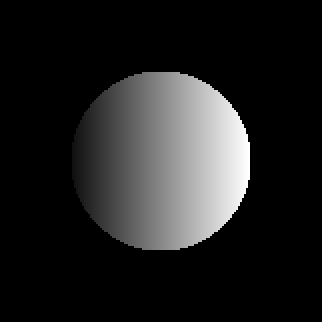
\includegraphics[width=0.3\textwidth]{images/demo/GACvsCV/inhom}	&

\includegraphics[height=0.3\textwidth]{images/demo/GACvsCV/GAC_inhom}	&
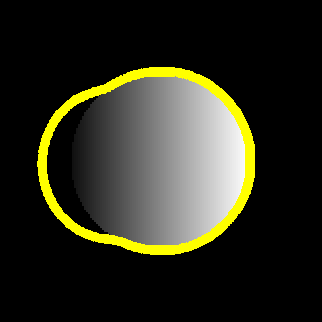
\includegraphics[height=0.3\textwidth]{images/demo/GACvsCV/CV_inhom}	\\
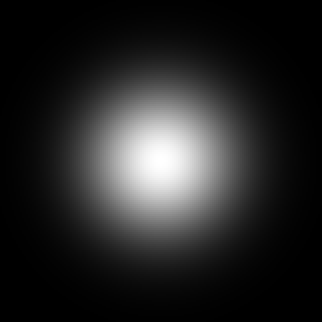
\includegraphics[width=0.3\textwidth]{images/demo/GACvsCV/gauss}	&
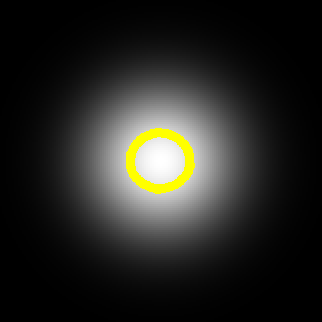
\includegraphics[height=0.3\textwidth]{images/demo/GACvsCV/GAC_gauss}	&
\includegraphics[height=0.3\textwidth]{images/demo/GACvsCV/CV_gauss}	\\
\includegraphics[width=0.3\textwidth]{images/demo/GACvsCV/gauss_noisy}	&
\includegraphics[height=0.3\textwidth]{images/demo/GACvsCV/GAC_gauss_noisy}	&
\includegraphics[height=0.3\textwidth]{images/demo/GACvsCV/CV_gauss_noisy}	\\
(a) simulated image & (b) GAC\cite{caselles_GAC} & (c) Chan-Vese\cite{chan_vese}
\end{tabular}
\caption[Edge based model vs region based model]{(a)Simulated images. (b)Segmentation performance of (GAC\cite{caselles_GAC}) and (c) Results via (Chan-Vese\cite{chan_vese}). The final result is shown by the yellow contour.}
\label{fig:GACvsCV}
\end{figure}
\clearpage
In the third example (Fig.~\ref{fig:GACvsCV}(a), row 3), the edges of the disc are blurred by smoothing it with a Gaussian filter. As expected, the edge based algorithm fails to identify the proper object boundary, whereas the region based technique performs significantly better.

Finally, the fourth image (Fig.~\ref{fig:GACvsCV}(a), row 4) is simulated by adding zero mean Gaussian noise to the blurry disc image. We observe that region based segmentation is particularly robust against additive noise and the segmentation performance is not degraded significantly. On the other hand, GAC model faces difficulties both due to blurred edges and due to noise.
\begin{figure}[t]
\centering
\renewcommand{\tabcolsep}{0.05cm}
\begin{tabular}{@{}ccc@{}}
\includegraphics[width=0.3\textwidth]{images/L2S_compare/orig_1}	&
\includegraphics[width=0.3\textwidth]{images/L2S_compare/GAC_1}	&
\includegraphics[width=0.3\textwidth]{images/L2S_compare/CV_1}	\\
\includegraphics[width=0.3\textwidth]{images/L2S_compare/orig_4}	&
\includegraphics[width=0.3\textwidth]{images/L2S_compare/GAC_4}	&
\includegraphics[width=0.3\textwidth]{images/L2S_compare/CV_4}	\\
\includegraphics[width=0.3\textwidth]{images/L2S_compare/orig_5}	&
\includegraphics[width=0.3\textwidth]{images/L2S_compare/GAC_5}	&
\includegraphics[width=0.3\textwidth]{images/L2S_compare/CV_5}	\\
(a) original image & (b) GAC & (c) Chan Vese
\end{tabular}
\caption[Geometric Snakes: negative examples]{Cases of improper segmentation using geometric contours. (a) Five images including simulated and real examples with varying illumination and weak edges. (b) Shows segmentation using geodesic active contour and (c) Shows segmentation due to Chan-Vese's method. The initial contour is plotted in green and the final contour in yellow. Intermediate steps of curve evolution are shown in cyan. This figure is best viewed in color.}
\label{fig:ls_compare}
\end{figure}
\subsection{Real examples}
In Fig.~\ref{fig:ls_compare}, a comparative study of segmentation performance of geodesic active contour model and Chan-Vese's technique is presented on a set of real images consisting of vascular structures. Fluorescence microscopy images are often plagued by noise, inhomogeneous intensity and low contrast which leads to weak and fuzzy edges. As a result, we find that neither \cite{caselles_geodesic} nor \cite{chan_vese} is perfectly suitable for segmentation under such conditions. Segmentation error is caused either due to the contour leakage phenomenon (Fig.~\ref{fig:ls_compare}(b)) or under segmentation (Fig.~\ref{fig:ls_compare}(c)). In the following chapter, we attempt to design a generic segmentation algorithm which is tolerant to the commonly occurring artifacts in fluorescence microscopy.
\section{Discussion} 
In this chapter we have provided a broad overview of geometric active contours. Geometric contours are topology adaptive which makes them particularly attractive choice for segmentation. The segmentation model is either described in terms of explicit curve motion equation (\ref{eq:curve_evolve_n&t}) and then implemented by implicit representation of the contour as the zero level curve of an embedding function (\ref{eq:explicit_motion_ls}). Another popular way to describe the segmentation process is via variational formulation which involves minimization of a suitable energy functional using variational calculus. The gradient flow equation (\ref{eq:variational_grad_flow}) is derived using gradient descent technique for computing the local minima of the functional. In either case, segmentation is performed by iteratively propagating the zero level set of the embedding function on a discrete grid using numerical techniques.

Both formulations are widely used in the community and they enjoy their own set of benefits. While curvature flow equations are often easy to conceptualize (e.g. equavalent to physical curve motion models such as wave propagation), variational models have gained popularity because of the flexibility to add further constraints in the solution in terms of shape prior. We also showed that in many cases it is possible to draw an analogy between the curve flow equations derived from the two techniques and in a majority of cases the results are  comparable.

We then presented a comparison between edge based and region based methods for segmentation. It is shown that edge based models are more suitable for high SNR images with prominent edges. Furthermore, such models are less susceptible to error if the object gray value is non homogeneous. Region based methods, on the other hand, are more robust to noise and do not depend particularly on the edge strength of the signal. However, it was demonstrated that the performance can degrade significantly in presence of intensity inhomogeneity. 

In the next chapter we focus our attention on segmenting vascular structures from 2D fluorescence microscopy images. As we have discussed briefly, fluorescence microscopy imagery are charecterized by poor contrast, fuzzy boundaries, and varying intensity levels of the object.  This restricts the performance of the popular traditional geometric active contour models. This motivates us to develop a geometric segmentation model which is capable of handling noise and contrast fluctuations in the images.


%% Chapter 3
%\setstretch{1} 
\chapter{Region based segmentation in presence of inhomogeneity} % Main chapter title
%\setstretch{1.5} 
\label{L2S_Ch} % For referencing the chapter elsewhere, use \ref{Chapter2} 

\lhead{Chapter 5. \emph{L2S}} % This is for the header on each page - perhaps a shortened title

%----------------------------------------------------------------------------------------
In the previous chapter we discussed the potential benefits of using geometric active contours for segmentation problems. Geometric snakes are capable of adapting to the topology of the objects and  their ability to elastically deform and delineate object boundaries with sub-pixel accuracy make these methods attractive choice for several biomedical image analysis applications. 

We have also illustrated how region based models are more suitable for segmenting noisy images with weak edges. One popular region based algorithm is due to Chan and Vese\cite{chan_vese} where the authors model the image as a set of flat zones or regions with constant gray value. The authors also propose a multi-phase variant \cite{vese_multiphase} of their approach to perform multi-class grouping. 

The constant illumination assumption is challenged in applications where the signal intensity is inhomogeneous. This is encountered frequently in many medical and biological imaging applications like magnetic resonance (MR) imaging, ultrasound, X-ray, confocal and electron microscopy, etc. While edge based techniques are better suited for non uniformly illuminated images, low SNR and weak edges of biological structures limit their general applicability.

\section{Application to 2D neuron tracing}

Before dealing with the 3D confocal images, which require more sophisticated processing, we first propose a segmentation algorithm which would work on relatively simpler 2D images. A 2D image is obtained from its 3D counterpart by taking a mean intensity projection along its vertical axis. Although the depth information is lost  when the image dimension is reduced by projecting it to a 2D space, there are several interesting issues which demand our attention even after this simplification. First, even after conversion  2D, we still retain substantial information about a neuron's morphology and this is why there exists a number of popular tracers which have been developed specifically for 2D processing \cite{basu2010tree2tree,meijering2004design}. Also, certain categories of neurons (e.g. the cells in the sub cuticle layer of  the Drosophila) exhibit flat topology, and for such applications 2D processing is more relevant.
Second, with the reduced dimension, one may perform computation at a much faster rate than in 3D, thereby making 2D analysis an attractive choice for an initial, global assessment of the neurites.  Finally, the 2D conversion introduces further challenges for image processing, including introduction of intensity inhomogeneity, which occurs due to signal attenuation by the tissues at greater depths. It is a challenge in itself to investigate the applicability of state of the art segmentation algorithms on these datasets and understand the special processing needs for further robust analysis.

\section{Background and motivation}
In this chapter we introduce an edge oblivious segmentation approach \emph{Legendre Level Set} (L2S), which is robust to smooth variations in region intensity levels. State of the art techniques that tackle inhomogeneity typically require some form of local processing. However, while a global method like Chan-Vese's is insufficient in handling large scale intensity variations, a strictly local approach may lead to undesired segmentation artifacts, especially in presence of noise. We aim to eradicate these issues by proposing a generalized solution for region based segmentation in presence of significant intensity variation and additive noise. 

Chan and Vese's region based technique is mathematically summarized in (\ref{eq:chan_vese}). The locally optimum level set embedding function $\phi^*$ that minimizes (\ref{eq:chan_vese}) partitions the image in two regions such that the foreground and background are best approximated by the scalars $c_1$ and $c_2$, which are computed using alternate minimization.

As mentioned previously, this model is incapable of handling spatially varying illumination. A solution was proposed in \cite{vese_multiphase}, where the authors replaced the scalars $c_1,c_2$  with smooth functions $c_1(\textbf{x})$ and $c_2(\textbf{x})$ in (\ref{eq:chan_vese_PS}).
\bea
\mathcal{E}_{CV}(\phi,c_1(\textbf{x}),c_2(\textbf{x}))&= \displaystyle\int_{\Omega}|f(\textbf{x})-c_1(\textbf{x})|^2\heav(\phi) d\textbf{x} + \int_{\Omega}|f(\textbf{x})-c_2(\textbf{x})|^2\heav(\phi) d\textbf{x} \nn
\\&+\displaystyle s_1\int_{\Omega}|\nabla c_1(\textbf{x})|d\textbf{x} + s_2\int_{\Omega}|\nabla c_2(\textbf{x})|d\textbf{x}
\label{eq:chan_vese_PS}
\eea
Smoothness of the functions are established by regulating their total variation, controlled by the parameters $s_1,s_2$. As before, alternating minimization is used to solve (\ref{eq:chan_vese_PS}). However, unlike (\ref{eq:chan_vese}), the polynomials are computed numerically, by deriving the EL equations and using gradient descent for local minimization.
%\bea
%\dfrac{\partial c_1(\textbf{x})}{\partial t} &=& 2(f(\textbf{x})-c_1(\textbf{x}))\heav
%(\phi) + s_1 \text{div}\left(\dfrac{\nabla c_1(\textbf{x})}{|\nabla c_1(\textbf{x})|}\right) \nn \\
%\dfrac{\partial c_2(\textbf{x})}{\partial t} &=& 2(f(\textbf{x})-c_2(\textbf{x}))\heav(\phi) + s_2 \text{div}\left(\dfrac{\nabla c_2(\textbf{x})}{|\nabla c_2(\textbf{x})|}\right)  \\
%\dfrac{\partial \phi}{\partial t} &=& \left[-(f(\textbf{x})-c_1^*(\textbf{x}))^2+(f(\textbf{x})-c_2^*(\textbf{x}))^2\right]\dirac(\phi) \nn
%\label{eq:PS_solution}
%\eea
\begin{gather}
\dfrac{\partial c_1(\textbf{x})}{\partial t} = 2(f(\textbf{x})-c_1(\textbf{x}))\heav
(\phi) + s_1 \text{div}\left(\dfrac{\nabla c_1(\textbf{x})}{|\nabla c_1(\textbf{x})|}\right) \nn \\
\dfrac{\partial c_2(\textbf{x})}{\partial t} = 2(f(\textbf{x})-c_2(\textbf{x}))\heav(\phi) + s_2 \text{div}\left(\dfrac{\nabla c_2(\textbf{x})}{|\nabla c_2(\textbf{x})|}\right)  \\
\dfrac{\partial \phi}{\partial t} = \left[-(f(\textbf{x})-c_1^*(\textbf{x}))^2+(f(\textbf{x})-c_2^*(\textbf{x}))^2\right]\dirac(\phi) \nn
\label{eq:PS_solution}
\end{gather}
While the solution is attractive, this piecewise smooth model is computationally expensive. This is because, in order to calculate the locally optimum level set function $\phi^*$, one needs to iteratively calculate the functions $c_1^*(\textbf{x})$ and $c_2^*(\textbf{x})$ by numerically solving (\ref{eq:PS_solution}) thereby making computation significantly expensive. 

Recently, Li \textit{et al}. \cite{li_region_scalable} introduced a region scalable model to localize the energy functional. The region localization is controlled by the scale of a Gaussian kernel, which is manually tuned for optimal performance. Efforts have been made to incorporate the region statistics for segmentation \cite{kim_nonparametric,cremers2007review}. These methods are robust to initialization and relatively less sensitive to noise. However, Lankton \textit{et al}.\cite{lankton_localCV} demonstrated that global statistics may not be the best resort for segmenting inhomogeneous objects. Instead, the authors generalize the local region based methods, by proposing a generic energy functional capable of performing segmentation using different region based criteria. 
They also show that by judiciously tuning the region localizing mask size, one can achieve high quality segmentation, even in presence of noise and inhomogeneity. 
However, one downside of their approach is that it requires additional local computation, thus increasing the risk of being stuck within local minima. 


Feng \textit{et al}.  \cite{feng2000tomographic} proposed a method for tomographic reconstruction by using a low order parametric model to represent object texture. However, the algorithm is tailored for tomographic reconstruction and is difficult to generalize. Recently a method was proposed to model the foreground and background by a linear function \cite{du_linear_approx}. This approach is an improvement over the model of Chan-Vese, but does not accommodate nonlinear illumination change.  

From the above discussion we observe that a majority of these approaches rely on local information only. While localizing the segmentation energy is essential in dealing with inhomegeneity, a generic global framework is also necessary to avoid the local minima problem. We propose to model the foreground and background illumination by a set of Legendre basis functions \cite{mukherjee_L2S}. This model allows the region intensities to be represented in a lower dimensional subspace, thereby permitting smooth approximation. Low dimensional signal representation has been used in a slightly different context in the literature, primarily to accommodate shape priors for segmentation \cite{fritscher20073d,huang2008metamorphs}.  However, although shape based information assists segmentation, such techniques require an atlas of pre-registered objects, which may be unavailable for general purpose segmentation. 
We further show that the proposed model \textit{Legendre Level Set} (or L2S) is computationally simple, since we achieve a stable, closed form solution at each iteration, allowing faster processing.

\section{2D segmentation using L2S}

The traditional Chan-Vese functional (\ref{eq:chan_vese}) can be reformulated and generalized by replacing the scalars $c_1$ and $c_2$ by   smooth functions $c_1^m(\textbf{x})$ and $c_2^m(\textbf{x})$. These functions are used to model the intensity in the two regions separated by the zero level set curves of $\phi$. The energy functional corresponding to the L2S data term is expressed as follows:
\bea
\mathcal{E}_{L2S}= \int_{\Omega}|f(\textbf{x})-c_1^m(\textbf{x})|^2H(\phi) d\textbf{x} 
						   +\int_{\Omega}|f(\textbf{x})-c_2^m(\textbf{x})|^2 \left(1-H(\phi)\right) d\textbf{x}  
\label{eq:L2S_data}
\eea
The essence of our approach is embedded in computing these functions. By allowing the regions to be modeled by flexible (but smooth) functions, we introduce the local information required to tackle the heterogeneous illumination. This is a notable feature of our algorithm. Unlike (\ref{eq:chan_vese_PS}), where smoothness is obtained by minimizing the total variation term, we only allow inherently smooth polynomials to approximate the region intensities. As we will show in the next few sections, this formulation allows a suitable framework to model the heterogeneity, without significantly sacrificing on computational time.

To preserve the smoothness and flexibility of the functions, we represent them as a linear combination of a few Legendre basis functions as shown below:
\bea
 c_1^m(\textbf{x}) &=& \sum_{k=0}^m\alpha_k\mathcal{P}_k(\textbf{x}) \\ c_2^m(\textbf{x}) &=& \sum_{k=0}^m\beta_k\mathcal{P}_k(\textbf{x})
 \label{eq:l2s_poly}
\eea
Here $\mathcal{P}_k$ is a multidimensional Legendre polynomial, which can be written as the outer product of the one dimensional counterparts. The 2-D polynomial is computed as $\mathcal{P}_k(x,y)=p_k(x)p_k(y)$, $\textbf{x}=(x,y)\in \Omega \subset [-1,1]^2$. $p_k$ is a one dimensional Legendre polynomial of degree $k$ defined as
\bea
p_k(x)=	\frac{1}{2^k}\sum_{i=0}^{k}\binom{k}{i}(x-1)^{k-i}(x+1)^i  
\label{eq:legendre}
\eea
The highest degree of the 1D bases is denoted by $m$. Hence, for the 2D case, we would represent the regions by a linear combination of a set of $(m+1)^2$ 2D Legendre basis functions.

\subsection{Optimization of the energy functional}
\begin{figure}[ht]
\centering
\captionsetup{justification=centering}
\renewcommand{\tabcolsep}{0.05cm}
\begin{tabular}{@{}ccc @{}}
	\includegraphics[width=.3\textwidth]{./images/Bases_color/1}  &
	\includegraphics[width=.3\textwidth]{./images/Bases_color/2}  &
	\includegraphics[width=.3\textwidth]{./images/Bases_color/3}  \\
	\includegraphics[width=.3\textwidth]{./images/Bases_color/4}  &
	\includegraphics[width=.3\textwidth]{./images/Bases_color/5}  &
	\includegraphics[width=.3\textwidth]{./images/Bases_color/6}  \\
	\includegraphics[width=.3\textwidth]{./images/Bases_color/7}  &
	\includegraphics[width=.3\textwidth]{./images/Bases_color/8}  &
	\includegraphics[width=.3\textwidth]{./images/Bases_color/9} 
\end{tabular}
\caption[2D Legendre polynomials]{The set of nine 2D Legendre basis functions. The 2D polynomials are computed from 1D functions of degree 2.}
\label{fig:legendre_bases}
\end{figure}

Let us denote $\mathbb{P}(\textbf{x})=\left(\mathcal{P}_0(\textbf{x}),\ldots, \mathcal{P}_{N-1}(\textbf{x})\right)^T$ as the vector of Legendre polynomials. $\textbf{a}=\left(\alpha_0,\ldots,\alpha_{N-1} \right)^T$ and $\textbf{b}=\left(\beta_0,\ldots,\beta_{N-1} \right)^T$ are the coefficient vectors for the two regions. $N=(m+1)^2$ is the total number of basis functions. We can now rewrite the modified version of (\ref{eq:chan_vese}) in matrix form as
\bea
\mathcal{E}(\phi,\textbf{a},\textbf{b})&= \displaystyle\int_{\Omega}\left[|f(\textbf{x})-\textbf{a}^T\mathbb{P}(\textbf{x})|^2 m_1(\textbf{x})+|f(\textbf{x})-\textbf{b}^T\mathbb{P}(\textbf{x})|^2m_2(\textbf{x}) \right]d\textbf{x} \nn \\
						    &+\lambda_1 ||\textbf{a}||_2^2  +\lambda_2 ||\textbf{b}||_2^2 + \nu\, \lint_{\Omega} |\nabla\heav(\phi)| d\textbf{x} 
\label{eq:leg_cv_mat}						  
\eea
In (\ref{eq:leg_cv_mat}) the last term introduces smoothness in the zero level curve, which is regulated by the parameter $\nu$.  Let us also denote  $m_1(\textbf{x})=\heav(\phi)$ and  $m_2(\textbf{x})=1-m_1(\textbf{x})$. 


The non negative regularizing parameters $\lambda_1,\lambda_2$ can be selected using cross validation techniques to avoid over-fitting.
The energy functional (\ref{eq:leg_cv_mat}) is optimized using alternating minimization. In the first step, to find the optimal coefficients, we take the partial derivative of (\ref{eq:leg_cv_mat}) with respect to $\textbf{a}$ and $\textbf{b}$ respectively and setting the result to zero. A closed form solution $\hat{\textbf{a}}$ and $\hat{\textbf{b}}$ is obtained as
\bea
\dfrac{\partial\mathcal{E}(\phi,\textbf{a},\textbf{b})}{\partial \textbf{a}}=0 \Rightarrow \hat{\textbf{a}} =& \left[K+ \lambda_1 \mathbb{I}\right]^{-1}\textbf{p} \\
\dfrac{\partial\mathcal{E}(\phi,\textbf{a},\textbf{b})}{\partial \textbf{b}}=0 \Rightarrow \hat{\textbf{b}} =& \left[L+ \lambda_2 \mathbb{I}\right]^{-1}\textbf{q} 
\label{coef_sol}
\eea
$\left[. \right]$ denotes a matrix. 
Here $\left[K \right]$ and $\left[L \right]$ are Gramian matrices \cite{gramian} of dimension $N\times N$, whose $(i,j)^{th}$ entry are obtained as follows:
\bea
\left[K\right]_{i,j}=& \left<\sqrt{m_1(\textbf{x})}\mathcal{P}_i(\textbf{x}),\sqrt{m_1(\textbf{x})}\mathcal{P}_j(\textbf{x})\right>=&\displaystyle \int_{\Omega}m_1(\textbf{x})\mathcal{P}_i(\textbf{x})\mathcal{P}_j(\textbf{x})d\textbf{x} \\
\left[L\right]_{i,j}=& \left<\sqrt{m_2(\textbf{x})}\mathcal{P}_i(\textbf{x}),\sqrt{m_2(\textbf{x})}\mathcal{P}_j(\textbf{x})\right>=&\displaystyle \int_{\Omega}m_2(\textbf{x})\mathcal{P}_i(\textbf{x})\mathcal{P}_j(\textbf{x})d\textbf{x}
\eea
Here $\left<,\right>$ denotes the inner product operator for real valued functions, and $0\leq i,j \leq N$. The individual elements $p_j$ and $q_j$ of the $N\times 1$ vectors  $\textbf{p}=\left(p_0,\ldots,p_N\right)^T$ and $\textbf{q}=\left(q_0,\ldots,q_N\right)^T$ are obtained as 
$
p_j=\lint_{\Omega} \mathcal{P}_j(\textbf{x})f(\textbf{x})m_1(\textbf{x})d\textbf{x} 
$ and 
$q_j =\lint_{\Omega} \mathcal{P}_j(\textbf{x})f(\textbf{x})m_2(\textbf{x})d\textbf{x}$ .
This can be written in a more compact form using vector notations as follows:
\bea
\textbf{p}=\lint_{\Omega} \mathbb{P}(\textbf{x})f(\textbf{x})m_1(\textbf{x})d\textbf{x} \label{eq:l2s_P}
\\
\textbf{q} =\lint_{\Omega} \mathbb{P}(\textbf{x})f(\textbf{x})m_2(\textbf{x})d\textbf{x}
\label{eq:l2s_Q}
\eea
With the updated coefficient vectors, we can now locally minimize (\ref{eq:leg_cv_mat}) with respect to $\phi$ borrowing techniques from variational calculus. 
The curve evolution is performed by numerically solving the following partial differential equation:
\bea
\frac{\partial \phi}{\partial t}=& \left[-|f(\textbf{x})-\hat{\textbf{a}}^T\mathbb{P}(\textbf{x})|^2 
						   +|f(\textbf{x})-\hat{\textbf{b}}^T\mathbb{P}(\textbf{x})|^2  + \nu \, \nabla \cdot\left(\dfrac{\nabla\phi}{|\nabla\phi|}\right) \right]\dirac(\phi)\nn\\
\label{eq:l2s_gradient_flow}
\eea
We solve (\ref{eq:l2s_gradient_flow}) using gradient descent and initializing $\phi|_{t=0}=\phi_0$ and $\dfrac{\dirac(\phi)}{|\nabla \phi|}\dfrac{\partial\phi}{\partial \hat{n}}=0$ at the domain boundary. See Appendix \ref{AppendixTuFF} for derivation of (\ref{eq:l2s_gradient_flow}).

\subsection{Analysis of L2S}
The surface approximate for foreground and background are obtained by computing $\hat{\textbf{a}}^T\mathbb{P}(\textbf{x})$ and $\hat{\textbf{b}}^T\mathbb{P}(\textbf{x})$. Since the coefficient vectors are available in closed form, it makes our algorithm fast and effective. The amount of intensity variation is governed by the coefficient vectors which are computed automatically. However, computing the coefficient vectors require a matrix inversion step. Here we show that the matrices $\left[K\right]$ and $\left[L\right]$ are invertible when the heaviside function is suitably regularized.

Since $\left[K\right]$ is a Gramian matrix, it is full rank iff the polynomials $\sqrt{m_1(\textbf{x})}\mathcal{P}_i(\textbf{x})$, $(i=1,\ldots,N)$ are linearly independent \cite{gramian}. Since the polynomials $\mathcal{P}_i(\textbf{x})$ are linearly independent themselves, it is easy to show that the linear independence holds if $0< m_1(\textbf{x})< 1$. A similar argument holds for analyzing the invertibility of $\left[L\right]$. In \cite{chan_vese}, the authors propose a regularized version of the heaviside function which is given by (\ref{eq:heav_relax})
By this definition, the functions $m_1(\textbf{x})$ and $m_2(\textbf{x})$ are bounded in $\left[0,1\right]$, which make the matrices invertible. 

However, inverting the above mentioned matrices may still be prone to numerical error  when $\sqrt{m_i(\textbf{x})}$ is small. The regularizing constants $\lambda_1$ and $\lambda_2$ contribute to make these matrices well conditioned. Furthermore, the regularization terms are necessary to avoid over-fitting. In most situations, we find that only a few (typically 16) 2-D Legendre functions are sufficient to model the region intensity. However, image noise may lead to over-fitting of the polynomials to the image segments, which may disrupt segmentation as the propagating level set may settle at a local minima. The scalars $\lambda_1,\lambda_2$ produce a damping effect by constraining the $\mathbb{L}_2$ norm of the bases coefficients, thereby favoring interior regions approximated by smooth functions. 

\subsection{Parameter selection for L2S}
Our algorithm requires specification of a few parameters, namely the Legendre polynomial degree $m$ and the regularizing constants $\lambda_1$ and $\lambda_2$ in (\ref{eq:leg_cv_mat}). We experimentally verified that the intensity variation in the images can be adequately modeled by using 1-D Legendre polynomials of (highest) degree three. We found that the algorithm is relatively robust to the selection of this value, but a higher degree polynomial typically requires inversion of a larger matrix, which makes computation significantly more expensive. To estimate the value of $\lambda_1$ and $\lambda_2$, we perform a \textit{leave one out} cross validation on each of the four categories in our dataset. The cross validation is performed over the values of $\{0,1,\ldots,100\}$ in multiples of 2. For simplicity, we have chosen $\lambda_1=\lambda_2$ for every experiment. The particular value which yields the highest average Dice coefficient for each dataset is chosen for experimentation. 


Automated selection of the contour smoothness parameter $\nu$ in (\ref{eq:leg_cv_mat}) is non-trivial. Typically, $0<\nu<1$, where a higher value produces smoother contour. As a rule of thumb, one may wish to set $\nu$ to a relatively higher value if the noise level in the image is high. For our experiments, we observe that the set of ultrasound images and the simulated noisy images require larger values of $\nu$. For all these images, we select $\nu=0.6$. For the less noisy images, $\nu$ is typically set in the range 0.05 to 0.2. 
 
\subsection{Comparison with GAC and Chan-Vese}
In Chapter 4, we introduced the edge based geodesic active contour\cite{caselles_geodesic} model and region based technique due to Chan and Vese \cite{chan_vese}. Fig.~\ref{fig:l2s_compare_GAC_CV} shows the performance of L2S versus GAC and Chan-Vese's method. To maintain fairness of comparison, we have initialized the level set at the same positions for each methods (shown by the green contour). All the five images used for this demonstration are characterized by low contrast, weak edges and significant variation in region illumination levels. 
\begin{figure}[t]
\centering
\renewcommand{\tabcolsep}{0.05cm}
\begin{tabular}{@{}cccc@{}}
\includegraphics[width=0.24\textwidth]{images/L2S_compare/orig_2}	&
\includegraphics[width=0.24\textwidth]{images/L2S_compare/GAC_2}	&
\includegraphics[width=0.24\textwidth]{images/L2S_compare/CV_2}		&
\includegraphics[width=0.24\textwidth]{images/L2S_compare/L2S_2}	
%\\
%\includegraphics[width=0.24\textwidth]{images/L2S_compare/orig_3}	&
%\includegraphics[width=0.24\textwidth]{images/L2S_compare/GAC_3}	&
%\includegraphics[width=0.24\textwidth]{images/L2S_compare/CV_3}		&
%\includegraphics[width=0.24\textwidth]{images/L2S_compare/L2S_3}	
\\
\includegraphics[width=0.24\textwidth]{images/L2S_compare/orig_1}	&
\includegraphics[width=0.24\textwidth]{images/L2S_compare/GAC_1}	&
\includegraphics[width=0.24\textwidth]{images/L2S_compare/CV_1}		&
\includegraphics[width=0.24\textwidth]{images/L2S_compare/L2S_1}	
\\
\includegraphics[width=0.24\textwidth]{images/L2S_compare/orig_4}	&
\includegraphics[width=0.24\textwidth]{images/L2S_compare/GAC_4}	&
\includegraphics[width=0.24\textwidth]{images/L2S_compare/CV_4}		&
\includegraphics[width=0.24\textwidth]{images/L2S_compare/L2S_4}	
\\
\includegraphics[width=0.24\textwidth]{images/L2S_compare/orig_5}	&
\includegraphics[width=0.24\textwidth]{images/L2S_compare/GAC_5}	&
\includegraphics[width=0.24\textwidth]{images/L2S_compare/CV_5}		&
\includegraphics[width=0.24\textwidth]{images/L2S_compare/L2S_5}	\\
(a) original image & (b) GAC & (c) Chan Vese & (d) L2S
\end{tabular}
\caption[L2S vs GAC vs Chan-Vese]{(a) A 2D image. Segmentation via (b) Geodesic active contour, (c)Chan-Vese and (d)L2S. The initial contour is plotted in green and the final contour in yellow. Intermediate steps of curve evolution are shown in cyan. Best viewed in color.}
\label{fig:l2s_compare_GAC_CV}
\end{figure}
GAC and Chan-Vese's algorithm's performance is limited due to these artifacts. GAC is prone to error due to weak edges causing contour leakage, whereas the piecewise constant model due to Chan and Vese is unable to accomodate the intensity inhomogeneities. However, we observe that L2S exhibits significantly superior qualitative performance since it is (a) not dependent on the edge information and (b) capable of handling discontinuities by using polynomial approximation for region intensities.

%\clearpage
\subsection{Comparison with other methods}
To demonstrate the efficacy of the proposed method, we perform further experiments on a dataset of 32 images. The dataset consists of a set of synthetic images with added noise and simulated intensity inhomogeneity, a set of biomedical images consisting of blood vessels using magnetic resonance angiogram (MRA), neurons and dendritic spines imaged by confocal microscope and finally, a set of ultrasound images of human blood vessels.  

To evaluate the performance of L2S, we compare our approach with three popular and widely used region based segmentation algorithms viz. Chan-Vese \cite{chan_vese}, Lankton et. al. \cite{lankton_localCV} and Li et. al.\cite{li_region_scalable}. We use the freely available CREASEG\cite{creaseg} tool to evaluate the performance. We choose the above techniques for performance evaluation since all the above models (barring Chan-Vese) were developed to perform region based segmentation with varying object brightness.

To set up the comparative evaluation procedure, we first present the segmentation results on a biomedical image dataset containing vascular structures. This is shown in Fig.~\ref{fig:l2s_compare_vessels}. Fig.~\ref{fig:l2s_compare_vessels}(a) shows the original microscopy images with the initial contour shown in yellow, followed by segmentation results due to (b) Chan-Vese in blue, (c) Lankton \textit{et al.} in red, (d) Li \textit{et al.} in cyan and finally (e) L2S (yellow). The images contains vascular structures and are characterized by  noise, non-object clutter and inhomogeneous intensity. To make a fair evaluation, the images were not preprocessed for contrast improvement or noise removal. 
\begin{figure*}[t]
\centering
\renewcommand{\tabcolsep}{0.05cm}
\begin{tabular}{@{}ccccc@{}}
\includegraphics[width=0.19\textwidth]{images/L2S_compare_region/19_orig}	&
\includegraphics[width=0.19\textwidth]{images/L2S_compare_region/19_CV}	&
\includegraphics[width=0.19\textwidth]{images/L2S_compare_region/19_Lankton}		&
\includegraphics[width=0.19\textwidth]{images/L2S_compare_region/19_Li}	&
\includegraphics[width=0.19\textwidth]{images/L2S_compare_region/19_ours}	
\\
\includegraphics[width=0.19\textwidth]{images/L2S_compare_region/22_trng_orig}	&
\includegraphics[width=0.19\textwidth]{images/L2S_compare_region/22_trng_CV}	&
\includegraphics[width=0.19\textwidth]{images/L2S_compare_region/22_trng_Lankton}		&
\includegraphics[width=0.19\textwidth]{images/L2S_compare_region/22_trng_Li}	&
\includegraphics[width=0.19\textwidth]{images/L2S_compare_region/22_trng_ours}	
\\
\includegraphics[width=0.19\textwidth]{images/L2S_compare_region/dendrites2_orig}	&
\includegraphics[width=0.19\textwidth]{images/L2S_compare_region/dendrites2_CV}	&
\includegraphics[width=0.19\textwidth]{images/L2S_compare_region/dendrites2_Lankton} &
\includegraphics[width=0.19\textwidth]{images/L2S_compare_region/dendrites2_Li}	&
\includegraphics[width=0.19\textwidth]{images/L2S_compare_region/dendrites2_ours}	
\\
\includegraphics[width=0.19\textwidth]{images/L2S_compare_region/n13_orig}	&
\includegraphics[width=0.19\textwidth]{images/L2S_compare_region/n13_CV}	&
\includegraphics[width=0.19\textwidth]{images/L2S_compare_region/n13_Lankton} &
\includegraphics[width=0.19\textwidth]{images/L2S_compare_region/n13_Li}	&
\includegraphics[width=0.19\textwidth]{images/L2S_compare_region/n13_ours}	
\\
\includegraphics[width=0.19\textwidth]{images/L2S_compare_region/neuron_clear_orig}	&
\includegraphics[width=0.19\textwidth]{images/L2S_compare_region/neuron_clear_CV}	&
\includegraphics[width=0.19\textwidth]{images/L2S_compare_region/neuron_clear_Lankton} &
\includegraphics[width=0.19\textwidth]{images/L2S_compare_region/neuron_clear_Li}	&
\includegraphics[width=0.19\textwidth]{images/L2S_compare_region/neuron_clear_ours}	
\\
\includegraphics[width=0.19\textwidth]{images/L2S_compare_region/spine2_orig}	&
\includegraphics[width=0.19\textwidth]{images/L2S_compare_region/spine2_CV}	&
\includegraphics[width=0.19\textwidth]{images/L2S_compare_region/spine2_Lankton} &
\includegraphics[width=0.19\textwidth]{images/L2S_compare_region/spine2_Li}	&
\includegraphics[width=0.19\textwidth]{images/L2S_compare_region/spine2_ours}	
\\
\includegraphics[width=0.19\textwidth]{images/L2S_compare_region/Vessel_CTA1_orig}&
\includegraphics[width=0.19\textwidth]{images/L2S_compare_region/Vessel_CTA1_CV}	&
\includegraphics[width=0.19\textwidth]{images/L2S_compare_region/Vessel_CTA1_Langton} &
\includegraphics[width=0.19\textwidth]{images/L2S_compare_region/Vessel_CTA1_Li}	&
\includegraphics[width=0.19\textwidth]{images/L2S_compare_region/Vessel_CTA1_ours}	
\\
\includegraphics[width=0.19\textwidth]{images/L2S_compare_region/vessel1_orig}	&
\includegraphics[width=0.19\textwidth]{images/L2S_compare_region/vessel1_CV}	&
\includegraphics[width=0.19\textwidth]{images/L2S_compare_region/vessel1_Lankton} &
\includegraphics[width=0.19\textwidth]{images/L2S_compare_region/vessel1_Li}	&
\includegraphics[width=0.19\textwidth]{images/L2S_compare_region/vessel1_ours}	
\\
\scriptsize(a)2D image&\scriptsize(b)Chan-Vese&\scriptsize(c)Lankton \textit{et al}\cite{lankton_localCV}&\scriptsize(d)Li \textit{et al}\cite{li_region_scalable}&\scriptsize(e)L2S
\end{tabular}
\caption[L2S on vascular images]{Qualitative comparison of L2S for vascular images.}
\label{fig:l2s_compare_vessels}
\end{figure*}
\clearpage

\begin{figure*}[t]
\centering
\renewcommand{\tabcolsep}{0.05cm}
\begin{tabular}{@{}ccccc@{}}
\includegraphics[width=0.19\textwidth]{images/L2S_compare_region/Degrade_orig}	&
\includegraphics[width=0.19\textwidth]{images/L2S_compare_region/Degrade_CV}	&
\includegraphics[width=0.19\textwidth]{images/L2S_compare_region/Degrade_Lankton}		&
\includegraphics[width=0.19\textwidth]{images/L2S_compare_region/Degrade_Li}	&
\includegraphics[width=0.19\textwidth]{images/L2S_compare_region/Degrade_ours}	
\\
\includegraphics[width=0.19\textwidth]{images/L2S_compare_region/SIM2_orig}	&
\includegraphics[width=0.19\textwidth]{images/L2S_compare_region/SIM2_CV}	&
\includegraphics[width=0.19\textwidth]{images/L2S_compare_region/SIM2_Lankton}		&
\includegraphics[width=0.19\textwidth]{images/L2S_compare_region/SIM2_Li}	&
\includegraphics[width=0.19\textwidth]{images/L2S_compare_region/SIM2_ours}	
\\
\includegraphics[width=0.19\textwidth]{images/L2S_compare_region/mushroom_orig}	&
\includegraphics[width=0.19\textwidth]{images/L2S_compare_region/mushroom_CV}	&
\includegraphics[width=0.19\textwidth]{images/L2S_compare_region/mushroom_Lankton} &
\includegraphics[width=0.19\textwidth]{images/L2S_compare_region/mushroom_Li}	&
\includegraphics[width=0.19\textwidth]{images/L2S_compare_region/mushroom_ours}	
\\
\includegraphics[width=0.19\textwidth]{images/L2S_compare_region/Airplane_orig}	&
\includegraphics[width=0.19\textwidth]{images/L2S_compare_region/Airplane_CV}	&
\includegraphics[width=0.19\textwidth]{images/L2S_compare_region/Airplane_Lankton} &
\includegraphics[width=0.19\textwidth]{images/L2S_compare_region/Airplane_Li}	&
\includegraphics[width=0.19\textwidth]{images/L2S_compare_region/Airplane_ours}	
\\
\includegraphics[width=0.19\textwidth]{images/L2S_compare_region/muscle_orig}	&
\includegraphics[width=0.19\textwidth]{images/L2S_compare_region/muscle_CV}	&
\includegraphics[width=0.19\textwidth]{images/L2S_compare_region/muscle_Lankton}		&
\includegraphics[width=0.19\textwidth]{images/L2S_compare_region/muscle_Li}	&
\includegraphics[width=0.19\textwidth]{images/L2S_compare_region/muscle_ours}	
\\
\includegraphics[width=0.19\textwidth]{images/L2S_compare_region/US3_orig}	&
\includegraphics[width=0.19\textwidth]{images/L2S_compare_region/US3_CV}	&
\includegraphics[width=0.19\textwidth]{images/L2S_compare_region/US3_Lankton} &
\includegraphics[width=0.19\textwidth]{images/L2S_compare_region/US3_Li}	&
\includegraphics[width=0.19\textwidth]{images/L2S_compare_region/US3_ours}	
\\
\includegraphics[width=0.19\textwidth]{images/L2S_compare_region/US7_orig}	&
\includegraphics[width=0.19\textwidth]{images/L2S_compare_region/US7_CV}	&
\includegraphics[width=0.19\textwidth]{images/L2S_compare_region/US7_Lankton} &
\includegraphics[width=0.19\textwidth]{images/L2S_compare_region/US7_Li}	&
\includegraphics[width=0.19\textwidth]{images/L2S_compare_region/US7_ours}	
\\
\includegraphics[width=0.19\textwidth]{images/L2S_compare_region/yeast_orig}	&
\includegraphics[width=0.19\textwidth]{images/L2S_compare_region/yeast_CV}	&
\includegraphics[width=0.19\textwidth]{images/L2S_compare_region/yeast_Lankton} &
\includegraphics[width=0.19\textwidth]{images/L2S_compare_region/yeast_Li}	&
\includegraphics[width=0.19\textwidth]{images/L2S_compare_region/yeast_ours}\\
\scriptsize(a)2D image&\scriptsize(b)Chan-Vese&\scriptsize(c)Lankton \textit{et al}\cite{lankton_localCV}&\scriptsize(d)Li \textit{et al}\cite{li_region_scalable}&\scriptsize(e)L2S
\end{tabular}
\caption[L2S on vascular images]{Qualitative comparison of L2S for non vascular images.}
\label{fig:l2s_compare_nonvessel}
\end{figure*}
\clearpage
We had mentioned earlier that one of our goals is to develop a segmentation procedure which is reasonably widely applicable. In this chapter we do not assume any structural prior for the objects to be segmented. Although prior information may achieve better results, the algorithm loses its general applicability. In the following chapter we will present a more problem specific solution to neuron segmentation. Since L2S is a general purpose segmentation algorithm, we also present qualitative results on non-vascular structures. However, almost all these images are characterized by inhomogeneous contrast, which is the major issue we try to address in this chapter. 

Segmentation results on a few representative images are  shown in Fig.~\ref{fig:l2s_compare_nonvessel}. This set of non vessel images belong to different categories. The first two images are simulated to contain a varying contrast and additive noise. We also include MRI images of human leg muscles, natural images from the Berkeley segmentation database\cite{BerkeleySegDatabase}, noisy ultrasound images of human arteries and finally microscopy images of yeast cells. As before, L2S results are shown in yellow and qualitative comparison suggest robustness of the method.

\subsection{Quantitative performance evaluation}
The Dice coefficient \cite{bernard_splinedCV} is used to quantify the results of segmentation. The Dice index $\mathcal{D}\in [0,1]$ between two regions $R_1$ and $R_2$ is given by 
\bea
\mathcal{D}(R_1,R_2)=2\dfrac{|R_1\cap R_2|}{|R_1|+|R_2|}
\label{eq:Dice}
\eea
Here $R_2$ is a binary image that denotes ground truth segmentation, and $R_1$ is the result obtained experimentally. A Dice index of 1 indicates perfect segmentation. The quantitative performance is shown in Fig.~\ref{fig:L2S_Dice}. 
\begin{figure}[t]
\centering
\includegraphics[width=1\textwidth]{images/L2S_Dice}
\caption[Quantitative comparison of L2S]{Dice index for the different algorithms are plotted in this bar chart. L2S results are shown by the yellow bar. Best viewed in color.}	
\label{fig:L2S_Dice}
\end{figure}
We observe that over this entire dataset, L2S yields an average Dice score of $0.9$, compared to $0.62,0.57$ and $0.7$ for the methods described in \cite{chan_vese},\cite{lankton_localCV} and \cite{li_region_scalable} respectively. 

\subsection{Computational comparison}
\begin{figure}[b]
\centering
\includegraphics[width=0.8\textwidth]{images/L2S_time}
\caption[Computational comparison for L2S]{The CPU running times (sec) for the different algorithms are plotted in this bar chart. L2S results are shown by the yellow bar. Best viewed in color.}	
\label{fig:L2S_comput}
\end{figure}
Our algorithm is implemented in Matlab and all experiments are performed on an Intel Pentium processor with 16 GB memory. The convergence times (in seconds) for the four algorithms are presented in Fig.~\ref{fig:L2S_comput}. Computationally, our method outperforms  \cite{lankton_localCV} and \cite{li_region_scalable} on average. It may be noted that the apparent low convergence time of \cite{chan_vese} often is a result of  convergence at local minima, which do not necessarily correspond to correct object boundaries.

\section{Discussion}
A novel framework for segmentation in presence of significant intra-region illumination variation is presented. Qualitative and quantitative results and comparison with the state of the art techniques suggest robustness of our approach. Here we have focused on bi-level segmentation, although extension to a multi-level framework appears straightforward. Also, our formulation allows easy incorporation of \textit{a priory} shape information, which may enhance performance in select cases. Salient highlights of L2S are presented below:
\begin{itemize}
\item L2S uses geometric active contours for segmentation. Therefore, it can adapt to the topological variations in objects via automatic merging and splitting.
\item L2S is robust against inhomogeneous intensity levels caused by non uniform signal attenuation or external bias fields, which occurs in many biological imaging applications. 
\item L2S is a region based method and its performance is robust against noise and weak edges.
\item L2S is computationally efficient and numerically stable.
\end{itemize}
However, like most level set methods, L2S is somewhat biased towards contour initialization. 
Also, although Legendre polynomials for region intensity approximation provides an elegant solution, it is difficult to comment on the optimality of this choice of bases. Effectiveness of other polynomials such as splines or wavelets \cite{achuthan2010wavelet} needs further investigation. In select cases, it may also be possible to learn a compact set of bases for representation. To address this issue, we identified a scenario  where a set of training examples of the object is available. We show that in such applications, the region approximating polynomials may be learned efficiently, instead of pre specifying them. This segmentation algorithm, \textit{Dictionary Learning Level Sets} (DL2S)\cite{sarkar_DL2S}, leverages the power of dictionary learning\cite{elad_ksvd} to learn the region approximating polynomials. We provide the details of DL2S in Appendix~\ref{AppendixDL2S}.

To develop a customized solution specifically for neuron tracing, we hypothesize that robust performance can be achieved by incorporating prior knowledge about the local shape of the neurites. While L2S is a general purpose, region based technique, in the following chapter we design a solution using level sets, that uses the local tubularity of the neurites to perform curve evolution.
 
%\chapter{Neuron Segmentation with Tubularity Flow Field} % Main chapter title

\label{TuFF_chapter} % For referencing the chapter elsewhere, use \ref{Chapter2} 

\lhead{Chapter 6. \emph{Tubularity Flow Field}} % This is for the header on each page 

In Chapter \ref{T2T2_chapter} and Chapter \ref{L2S_Ch}, we have discussed two segmentation algorithms. The first method, Tree2Tree-2 is a graph based tracer, which performs neuron tracing by identifying the correct connections between the neurite fragments after an initial segmentation. We remarked in Chapter \ref{T2T2_chapter}, that Tree2Tree-2 encounters difficulties when the neurons exhibit complicated morphology, and it predicts false connections. This motivated us to use geometric active contours, so that the connectivity handling could be performed implicitly. This led to the region based segmentation algorithm L2S, which is primarily designed for 2D applications where the region intensities are inhomogeneous. 

While L2S overcomes the false connectivity problem of Tree2Tree-2, it is essentially a generalized segmentation technique, and we hypothesize that adopting domain specific knowledge in the framework would make neuron segmentation more robust. This motivates our proposed solution, where level sets are used for segmentation, but the energy functional is designed specifically for segmenting tubular structures, both in 2D and 3D.

\section{Introduction}
\begin{figure}[t]
\centering
\includegraphics[width=0.7\linewidth]{./images/TuFF/discontinuities}
\caption[Gaps in neuron structures]{Maximum intensity projection of a neuron imaged by a confocal microscope. The image suffers from contrast non-uniformity, including gaps that lead to breaks in the segmented neurite structure. The effect is most pronounced in the region bounded by yellow dashed box, magnified here for improved viewing.}
\label{fig:discontinuities}
\end{figure}
As earlier, we restrict ourselves to reconstructing single neurons from  confocal microscopy. A robust neuron segmentation scheme needs to address two primary issues. 
\begin{itemize}
\item First, the technique should  be suited to identify neuron structures from the noisy confocal images. This requires a specialized procedure for clutterand noise removal, while preserving the filamentous structures of the neurites. 
\item Second, it should be adept at handling the local structure discontinuities (see Fig. \ref{fig:discontinuities}) resulting from imaging artifacts and pre processing errors. While Tree2Tree-2 used explicit schemes for joining such broken branches, we leverage the capabilities of geometric active contours to do the same.
\end{itemize}
We propose a solution to this segmentation problem using a variational framework driven by geometric active contours. The level set evolution is guided by minimizing an application specific energy functional. A tubularity flow field (TuFF) is computed by utilizing the local tubularity of the neurites which guides the segmentation procedure by encouraging curve evolution along the length (axis) and the thickness of the tubular neurites. A specialized local attraction force is also designed to accommodate the intensity variations in the images of neurite structures, thus presenting an unified framework to naturally link the fragmented structures. Our method does not rely on an initial set of seed-points for segmentation; it is automatic. Moreover, it does not require non-trivial post-segmentation analysis to link the disjoint segments. This is performed naturally by using the local attraction force in a level set paradigm. This enables us to connect disunited structures, even if the underlying signal intensity is significantly low. The problem  formulation and the design process of the attraction force are discussed in the following sections. 

\section{Tubularity Flow Field for neuron segmentation}
Let $f:\Omega \rightarrow \mathbb{R}$ be an image defined on the continuous domain $\Omega \subset \mathbb{R}^d$, where $d$ is the dimension of the image. We propose a solution in a variational paradigm, where implicit motion of the zero level set of the embedding function $\phi$ is obtained by (locally) minimizing an energy functional $\mathcal{E}(\phi)$. 
\begin{figure}[t]
\centering
\subfigure[]{
\includegraphics[width=.21\linewidth]{./images/TuFF/n12_speckle}
}
\subfigure[]{
\includegraphics[width=.21\linewidth]{./images/TuFF/n12_Otsu_2}
} 
\subfigure[]{
\includegraphics[width=.21\linewidth]{./images/TuFF/n12_ChanVese}
}
\subfigure[]{
\includegraphics[width=.21\linewidth]{./images/TuFF/MFVF_2}
}

\caption[Global segmentation of neurites]{(a) A 2-D neuron subimage. (b) and (c) show segmentation results using Otsu's method and the Chan-Vese variational technique respectively. Fragmented segmentation output is observed in (b) and (c) due to the non-local behavior of the algorithms. (d) Segmentation using TuFF (the proposed method).}
\label{fig:CV_compare}
\end{figure}
For this problem of neuron segmentation, we need to design the energy functional such that it would encourage curve propagation in the filamentous regions of the image, while avoiding the non tubular structures. Also, the segmentation should allow sufficient local processing to avert fragmented segments in the solution, which may appear as a consequence of using global threshold selection schemes like that of Otsu \cite{otsu} or methods assuming piecewise constant intensity models of \cite{chan_vese} (see Fig.~\ref{fig:CV_compare}).  We avoid this problem  by introducing a local shape prior by way of a specially designed tubularity flow vector field and a local  attraction force  to link nearby neuronal fragments.

\subsection{Tubularity Flow Field (TuFF)}
In Chapter \ref{T2T2_chapter}, we defined the concept of tubularity flow field (TuFF). This vector field consists of the set of orthonormal vectors $\{\textbf{e}_i(\textbf{x})\}$. The vectors are ordered according to increasing magnitude of curvatures, which are given by the scalars $\{|\lambda_i|\}$. We showed in Chapter \ref{T2T2_chapter}, that one popular procedure of obtaining these vector fields is via eigen analysis of the  hessian matrix of the Gaussian  filtered image. Frangi\cite{frangi_vesselness} suggested a multiscale procedure to distinguish vascular structures from background by using a multiscale vesselness function $N(\textbf{x})$. One such choice of a vesselness function is given in (\ref{eq:vesselness_scale}). 

The vesselness function $N(\textbf{x})$ helps distinguishing filamentous structure from noise and clutter, where its value is close to zero.  Clutter are present in most confocal microscopy images due to photon emission from non neuronal tissues and are often referred to as \emph{structure noise}. These structure noise may be bright disc shaped non-neuronal segments in 3D images or blob shaped structures. In the following subsections, we show how TuFF can be incorporated in a level set framework to perform neuron segmentation.

\subsection{Variational formulation with TuFF}
Our method performs segmentation via minimization of the energy functional $\mathcal{E}(\phi)$. This energy functional can be mathematically written as:
\bea
	\mathcal{E}(\phi)&=&\mathcal{E}_{reg}(\phi)+\mathcal{E}_{evolve}(\phi)+\mathcal{E}_{attr}(\phi)
	\label{eq:total_energy} \\
	\mathcal{E}_{reg}(\phi)&=&\nu_1\int_{\Omega}|\nabla H(\phi)|d\textbf{x} 
		\label{eq:smooth_energy}  \\ 
		\mathcal{E}_{evolve}(\phi)&=&-\int_{\Omega}\sum_{i=1}^{d}\alpha_i(\textbf{x})\langle\textbf{e}_i(\textbf{x}),\textbf{n}(\textbf{x})\rangle^2 H(\phi)d\textbf{x}
			\label{eq:evolve_energy}
\eea
Here $\mathcal{E}_{reg}$ and $\mathcal{E}_{evolve}$ are the energy functionals corresponding to the smoothness of the curve and the curve evolution respectively. The functional $\mathcal{E}_{attr}$ contributes towards creating a local attraction energy. This attraction energy is to be designed in a manner such that minimizing it would result in a force field to join the local, disjoint neuron fragments. For our application, we do not define the attraction energy explicitly; instead, we compute the attraction force resultant from the energy. This is discussed in Sec. 6.3.

The vector $\textbf{n}(\textbf{x})=-\dfrac{\nabla\phi(\textbf{x})}{|\nabla\phi(\textbf{x})|}$ denotes the outward unit normal  vector to the level sets of $\phi$. $\langle \cdot,\cdot \rangle$ is the Euclidean inner product operator. The positive scalar $\nu_1$ in (\ref{eq:smooth_energy}) contributes to the smoothness of the zero level curve. The weighing parameter $\alpha_i$ determines the contribution of the orthogonal and axial components of the TuFF in curve evolution. Choice of $\alpha_i$ is an important aspect which would be discussed shortly. 

In practice, the ideal Dirac delta function $\delta(\phi)$ and the Heaviside function $H(\phi)$ are replaced by their regularized counterparts $\dirac(\phi)$ and $\heav(\phi)$ respectively.

\subsection{TuFF gradient flow equation}
The essence of our technique lies in the design of curve evolution energy $\mathcal{E}_{evolve}$ in (\ref{eq:evolve_energy}). In absence of the attraction force energy, the level curve evolution (which results from minimizing the energy term (\ref{eq:evolve_energy})) depends on the contribution of the axial and orthogonal components of the tubularity flow field. The design of the functional (\ref{eq:evolve_energy}) is such that the axial vector field component $\textbf{e}_1$ is responsible for propagating the curve to fill out the vessel thickness. Or in other words, the axial field promotes curve evolution in a direction perpendicular to itself. Identically, the orthogonal components $\textbf{e}_2,\textbf{e}_3$ encourage curve propagation in a direction perpendicular to themselves, i.e. along the axis of the neuron filaments. Let us discuss the effect of tubularity flow field on contour propagation in the following subsection. For simplicity, only a 2D case is discussed, but the extension to 3D follows similar arguments.

\subsubsection{Effect of the axial component of TuFF}
\begin{figure}[t]
\renewcommand{\tabcolsep}{0.05cm}
\begin{tabular}{cc}
	\includegraphics[width=.45\linewidth]{./images/TuFF/tangential_graphic}
	&\includegraphics[width=.45\linewidth]{./images/TuFF/normal_graphic}
	\\
	\scriptsize (a) & \scriptsize (b) 
\end{tabular}
\caption[Graphic illustration of TuFF]{ Illustration of curve evolution due to (a) axial component $\textbf{e}_1$ and orthogonal component (b) $\textbf{e}_2$. Note how the contour should change to align the surface normals (shown in red arrow) with the vector fields (shown in green and purple arrows respectively) to minimize the evolution energy. The initial curve is marked as 1. The evolution forces create the new curves 2. Note how the curves assume elliptical shape to align the level set normals with the vector fields. The normal vectors are maximally aligned in the region enclosed by the rectangles.}
\label{fig:evolve_graphic}
\end{figure}
Maximizing the total squared inner product 
$\displaystyle \int_{\Omega}\alpha_1(\textbf{x})\langle \textbf{e}_1(\textbf{x}),\textbf{n}(\textbf{x})\rangle^2\heav(\phi)$ 
(or minimizing its negative) with respect to the embedding function $\phi$ results in maximally aligning the  outward normal vectors $\textbf{n}(\textbf{x})$ of the zero level sets of $\phi$ and its inner isocontours  with the axial flow field $\textbf{e}_1(\textbf{x})$. This requires the level sets of $\phi$ to be re-aligned such that the normal vectors $\textbf{n}(\textbf{x})$ aligns itself with the axial field $\textbf{e}_1(\textbf{x})$. This results in curve evolution in a direction orthogonal to the vessel axis, causing elongation of the level curves along the vessel width. 

\subsubsection{Effect of the orthogonal component of TuFF}
Using a similar argument, maximizing the second term corresponding to the orthogonal component in (\ref{eq:evolve_energy}) performs alignment of the outward normal vectors with the  vector field $\textbf{e}_2(\textbf{x})$, creating  an elongation force which allows the level curves to propagate along the vessel axis. For an intuitive understanding of the above mentioned phenomenon, Fig.~\ref{fig:evolve_graphic}(a) and (b) is provided to graphically demonstrate how the curve evolution is affected by the axial and the normal components of TuFF. 

\subsubsection{Effect of the vector field weights}
Ideally, the parameters $\alpha_i(\textbf{x}),i=1,\ldots,d,$ should be chosen such that curve propagation is discouraged outside the tubular neurite segments, so as to avoid leakage into the background. i.e. for a voxel $\textbf{y}$ with low vesselness score,  we require $\alpha_i(\textbf{y})\approx 0$, for $i=1,\ldots,d$. Moreover, since the neurites are elongated structures, it is desired that the contour evolution be more pronounced near the filament centerline than at the edges. This can be stated as 
\bea \label{eq:alpha_ratio}
\frac{\alpha_j(\textbf{x})}{\alpha_1(\textbf{x})} \geq 1 \;\; (j=2,\ldots,d)  \;\;\; \text{and}\;\; \alpha_1(\textbf{x}),\ldots,\alpha_d(\textbf{x})>0
\eea
Respecting the above constraints, we propose the following functions for choosing the parameters.
\begin{gather}
\alpha_1(\textbf{x})=N(\textbf{x})\label{eq:alpha1_choice}\\
\alpha_j(\textbf{x})=N(\textbf{x})\left(a_0+\exp\left(-\frac{|\nabla_{\sigma}f(\textbf{x})|}{a_1}\right)^2\right)
\label{eq:alpha2_choice}
\end{gather}
$\forall \textbf{x}\in\Omega$ and  $j=2,\ldots,d$. $N(\textbf{x})$ is the  vesselness score which is obtained from (\ref{eq:vesselness_scale}). 

\subsubsection{Isotropic TuFF equation}
Let us discuss the isotropic case, when $a_0=1$ and $a_1\to \infty$. 
Since the unit normal vector $\textbf{n}(\textbf{x})$  lies in the vector space spanned by $\{\textbf{e}_i(\textbf{x})\}$, it can  be written as $\textbf{n}(\textbf{x})=\displaystyle \sum_{i=1}^{d}m_i\textbf{e}_i(\textbf{x})$. This reduces (\ref{eq:evolve_energy}) to 
\bea
\mathcal{E}_{evolve}(\phi)=-\int_{\Omega}N(\textbf{x})\sum_{i}\langle\textbf{e}_i(\textbf{x}),\sum_{j}m_j\textbf{e}_j(\textbf{x}))\rangle^2 H_\epsilon(\phi)d\textbf{x}
\eea
Since the eigenvectors are orthonormal, $\langle\textbf{e}_i,\textbf{e}_j\rangle=1$ if $\textbf{e}_i,\textbf{e}_j\neq \textbf{0}$ and $i=j$, and 0 otherwise. Also, since $|\textbf{n}(\textbf{x})|=1$, we have $\sum_{i} m_i^2=1$. Using this relation, we obtain $\sum_{i}\langle\textbf{e}_i(\textbf{x}),\sum_{j}m_j\textbf{e}_j(x))\rangle^2=1$. This reduces the evolution equation to
\bea
\mathcal{E}_{evolve}(\phi)=-\int_{\Omega}N(\textbf{x})H_\epsilon(\phi)d\textbf{x}
\label{eq:isotropic_evolve}
\eea
The energy functional in (\ref{eq:isotropic_evolve}) when minimized performs segmentation via vesselness weighted isotropic region growing along the neuron segments. Leakage of the contour outside vessel boundaries is prohibited by the vessel indicator function $N(\textbf{x})$ which provides evidence of tubularity by assuming higher value for the tubular objects than non tubular background.


With the discussion of the isotropic case, it is now easier to visualize the effect of the weights on curve evolution. From our previous discussion, we recall that  $\alpha_1$ and $\{\alpha_j, j\neq 1\}$ influence curve propagation along the vessel width and axial direction respectively.  $|\nabla_{\sigma}f(\textbf{x})|$ denotes the gradient magnitude of the image $f(\textbf{x})$, which is filtered by a Gaussian kernel with variance $\sigma^2$. Since this term is high at the vessel boundaries and end points, the negative exponential term in (\ref{eq:alpha2_choice}) ensures higher response at regions near the vessel centerline. The tuning parameters $a_0 \ge 1$ and  $a_1$ determine the relative influence of the axial curve motion to the motion along the vessel width.  In other words, in an anisotropic setting, (\ref{eq:alpha2_choice}) suggests that  the level curves evolve with higher curvature near the vessel medial axis than at  the  edges, which percolates to the isotropic case when $a_0=1$ and $a_1\to \infty$. 

Since the neurite filaments are predominantly thin, elongated structures, we observe that  the isotropic case yields sufficiently appropriate segmentation results when the initialized zero level set encompasses the filament width. Nevertheless, the proposed framework in (\ref{eq:total_energy}) is general, and is applicable to segmentation problems where vessel thickness is significant and the initialized zero level contour does not fill out the vessel width completely. This is in contrast to the approach in \cite{shang2011vascular}, where segmentation of thicker vessels needs separate treatment. 

\subsection{Minimization of the TuFF functional}
The energy functional in (\ref{eq:total_energy}) can be minimized using variational calculus techniques \cite{calc_of_var}. Taking the G{\^a}teaux variation of $\mathcal{E}(\phi)$ with respect to $\phi$, we obtain from (\ref{eq:total_energy})
\begin{align}
	\nabla_\phi \mathcal{E} =\nabla_\phi \mathcal{E}_{reg}+\nabla_\phi \mathcal{E}_{evolve}+\nabla_\phi \mathcal{E}_{attr}
\label{eq:gateaux}
\end{align}
$\phi$ can be iteratively updated using gradient descent technique, i.e. setting $\nabla_\phi \mathcal{E}=-\dfrac{\partial\phi}{\partial t}$ with $t$ denoting the pseudo time parameter for the iterative scheme:
\bea\label{eq:total_force_eqn}
\frac{\partial\phi}{\partial t}=\mathcal{F}_{reg}(\textbf{x})+\mathcal{F}_{evolve}(\textbf{x})+\mathcal{F}_{attr}(\textbf{x})
\eea
$\mathcal{F}_{reg}$ and $\mathcal{F}_{evolve}$ are scalar force functions, which resulting from locally minimizing the regularizing energy and the evolution energy functionals. These forces are derived by solving the  Euler-Lagrange equation for level set evolution in the following manner:
\bea
	\mathcal{F}_{reg}(\textbf{x})&=&\nu_1 \, \text{div}\left(\textbf{n} \right)\dirac(\phi) \label{eq:reg_force}\\
	\mathcal{F}_{evolve}(\textbf{x})&=&\dirac\left(\phi\right)\sum_{j=1}^{d}\{\alpha_j(\textbf{x})\beta_j^2\left(\textbf{x} \right)\}- \nn\\
	&& 2\;\rm{div}\left(\sum_{\mathit{j}=1}^{\mathit{d}}\eta_{\mathit{j}} (\textbf{x})\left(\textbf{v}_j(\textbf{x})-\beta_{\mathit{j}} \left(\textbf{x}\right)\textbf{n}(\textbf{x})\right)\right) \nn\\
	\label{eq:evolve_force}
\eea
The coefficients $\beta_j$ and $\eta_j$ are defined as follows:
\bea
	\beta_j(\textbf{x})&=&\langle \textbf{v}_j(\textbf{x}),\textbf{n}\left(\textbf{x}\right)\rangle \\
	\eta_j(\textbf{x})&=&\alpha_j(\textbf{x})\beta_j(\textbf{x})\dfrac{\heav(\phi)}{|\nabla \phi|}
\eea 
The derivation details are shown in Appendix \ref{AppendixTuFF}.

\section{Local attraction force field}
The attraction force $\mathcal{F}_{attr}$ in (\ref{eq:total_force_eqn}) is introduced to accommodate the signal intensity variation (and signal loss) across the neurite branches, as shown in  Fig.~\ref{fig:discontinuities}. Such signal attenuation introduces unwarranted discontinuities in the filamentous objects, resulting in disjoint fragments.
Also, discontinuities may be present at the neurite junctions and noisy regions due to the nonlinear response of the vesselness function in (\ref{eq:vesselness_scale}). In such a scenario, the TuFF based evolution energy term in (\ref{eq:evolve_energy}) is not adequate by itself to perform segmentation. This insufficiency motivates the inclusion of an attraction force component. Designing this attraction force requires analysis of the connected components at each time epoch of level set propagation. At a time $t$ for evolution of the embedding function, the set of connected components $\mathcal{C}(t)$ are obtained as: 
\bea
	\mathcal{C}(t)=H\left(\phixt \right) \\
	\text{where $H(y)=$}\nn
	\begin{cases}
		1 & \text{for $y\geq0$}\\
		0 & \text{$y<0$}
	\end{cases}
\eea
The set of connected components $\mathcal{C}(t)=\{c_1,\ldots,c_p\}$ represents the binary segmentation at time $t$, which consists of $p\geq1$ disjoint connected components. Note that this binarization does not require a sophisticated segmentation, since the binary components are obtained by extracting the interior of the zero level sets of the embedding function. Each disjoint component $c_j$ is a potential candidate or a \emph{parent} which has the capability of attracting the remaining \emph{children} $c_k$, 
$k\ne j$,$\left(j,k= 1,\ldots,p\right)$. This is illustrated in Fig.~\ref{fig:attr_force}(a)-(c), where the component $c_1$ acts as a parent component and $c_2$ and $c_3$ are the children.
\begin{figure}[t]
\centering
\subfigure[]{
		\includegraphics[width=.31\linewidth]{./images/TuFF/attr_force/all}
}\hspace{-0.2cm}
\subfigure[]{
		\includegraphics[width=.31\linewidth]{./images/TuFF/attr_force/CH_master}
}\hspace{-0.2cm}
\subfigure[]{
		\includegraphics[width=.31\linewidth]{./images/TuFF/attr_force/slaves}
}\hspace{-0.2cm}
\\
\centering
\subfigure[]{ %
	\includegraphics[width=0.7\linewidth]{./images/TuFF/attr_force/force_field}
}
\caption[Graphic illustration of local attraction force field]{(a) Set of disjoint connected components $\{c_1,c_2,c_3\}$ at a particular step of iteration. (b) shows a parent component, the green dotted line marking its convex hull. The remaining children are shown in (c). (d) shows the attraction force obtained via (\ref{eq:Attr_Field}) in red arrows, magnified for visual clarity.}
\label{fig:attr_force}
\vspace{-0.2in}
\end{figure}

\subsection{Candidate points for attraction force field}
The primary responsibility of the attraction force is to enable the propagating contour surface to attach itself to local disjoint fragments. However, not all points on the connected components are candidates for creating the attraction force. This is because in a majority of the prevalent discontinuities, at least one of the two disconnected portions are likely to be joined via boundary points which represent region of high curvature (see Fig.~\ref{fig:disc_types}). 
If we denote the boundary of a component $c_j$ by $\delta c_j$, to enable a parent to attract a child, we need to design an attraction field which is generated by a set of candidate points lying on the parent boundary. 
Therefore, for a parent component $c_j$, a point $\textbf{y}\in \delta c_j$ belongs to the candidate set if $\textbf{y}$ is a point the convex hull \cite{convex_hull_graham} $\mathcal{H}_j$  of $c_j$ (Fig.~\ref{fig:attr_force}(b)). Formally, the candidate point set $\mathcal{M}_j$ for the connected component $c_j$ is defined as
\bea
\mathcal{M}_j=\{\textbf{y}\in \delta c_j:\exists \:\textbf{x}_j \in \mathcal{H}_j \;\; \text{s.t.}\; \|\textbf{y}-\textbf{x}_j\|_2\leq \Delta\}
\eea
$\Delta$ is a positive parameter that includes local boundary coordinates of the neighboring points on the convex hull. 

\subsection{Attraction force field design}
The candidate set of points for a parent component is responsible for generating a force field capable of attracting the candidate children towards itself for potential merging. This needs to be designed such that the attraction field vectors point toward the region of interest, which is the parent candidate point set for this purpose. We show that an efficient solution may be obtained by using vector field convolution (VFC) to create the attraction force field.

VFC \cite{li_VFC} is a technique primarily designed to create smooth external force field for parametric active contours. The specially designed vector field kernel (\ref{eq:VFC}) generates the desired external force when convolved with the object edge map, with the capability of attracting a contour to the region of interest.
\bea
	\textbf{K}(\textbf{p})=&-m(\textbf{p})\frac{\textbf{p}}{\|\textbf{p}\|} \nn\\
%	m(\textbf{p})&=&\|\textbf{p}\|^{-\gamma}
	m(\textbf{p})=&\exp(-||\textbf{p}||^{2}/\gamma^{2})
	\label{eq:VFC}
\eea
$\textbf{p}=\bf 0$ denotes the kernel center. The capture range of the vector field is controlled by the parameter $\gamma$. 

The set of candidate points $\mathcal{M}_j$ for a parent $c_j$ serves as the region of interest to which other components are likely to be attracted. Performing convolution of the candidate set with the kernel in (\ref{eq:VFC})  results in a vector field where the vectors are directed toward the parent, their magnitude attenuating gradually with distance from the candidate set.
If $E_j(\bf x)$ is a binary edge-map which assumes a value of $1$ only at points in $\mathcal{M}_j$, we can obtain the attraction force field  $\Gamma_j$ due to the parent $m_j$ as
\bea
\label{eq:Attr_Field}
\Gamma_j(\textbf{x})=E_j(\textbf{x})\ast \textbf{K}(\textbf{x}), \quad \forall \textbf{x}\in \Omega.
\eea
The nature of the attraction force field can be intuitively understood from Fig.~\ref{fig:attr_force}. Fig.~\ref{fig:attr_force}(a)  shows three connected components and the representative parent $c_1$ enclosed by its convex hull (shown in (b)). Fig.~\ref{fig:attr_force}(c) illustrates the attraction force field due to the parent as the red arrows which are oriented in the direction of the parent component. The capture range, which is specified by $\gamma$, is shown by the red region. 

Adopting this policy for designing the attraction field enjoys a few benefits. First, with a specified capture range, we can impose a locality in the approach, by discouraging distant segments to be connected to the parent. As $\gamma$ increases, effect of the attraction force field gradually diminishes as one moves further from the parent. Moreover, the candidate set is chosen such that only the convex portions of the parent boundary are capable of generating the force field. This ensures not all local structures are potential candidates for linking. For example, in Fig.~\ref{fig:attr_force} the component $c_3$ is not in the capture range of the force field of $c_1$, although it resides in the parent's local neighborhood. To summarize, the attraction force field is designed such that it may attract local connected components which are present in near vicinity of the parent's boundary convexity.  

\subsection{Attraction force}
For a parent-child pair $c_i$ and $c_j$, the parent attracts the child with a force $\mathcal{F}_{attr}^{(i,j)}$ given by
\bea
\mathcal{F}_{attr}^{(i,j)}(\textbf{y})=\mathcal{M}_i\langle \Gamma_i(\textbf{y}),-\textbf{n}(\textbf{y})\rangle \theta_j(\textbf{y})
\label{eq:attr_force_ij}
\eea
The indicator function $\theta_j(\textbf{y})=1$ if $\textbf{y}\in \delta c_j$ and $0$ otherwise. $\mathcal{M}_i$ is the normalized mass of the component $c_i$ which is computed as the ratio of the number of pixels/voxels in $c_i$ to the total pixels/voxels in $\{c_1,\ldots,c_p\}$. The inner product term in (\ref{eq:attr_force_ij}) suggests that higher force of attraction is experienced by a point on a child's boundary if the outward normal at that point is oriented along the attraction field.  


By introducing the factor $\mathcal{M}_i$, we equip heavier connected components with more attractive power.
Assuming that the neurites occupy larger volume than the noisy background voxels, we clean the solution of the level set function by performing an area opening operation which eliminates small components with area less than a pre defined threshold \cite{acton_fast}. This filtering operation avoids undesired objects to participate in the attraction force field computation. Now, for each parent-child pair in the filtered component space, we can compute the total attraction force $\mathcal{F}_{attr}$ in (\ref{eq:total_force_eqn}) as
\bea
\mathcal{F}_{attr}(\textbf{y})=\nu_2\sum_{i=1}^{p}\sum_{j\neq i}^{p}\mathcal{F}_{attr}^{(i,j)}(\textbf{y}),\quad
\forall \textbf{y}\in \Omega.
\label{eq:total_attr_force}
\eea
The positive scalar $\nu_2$ determines the effect of the attraction force on curve evolution. A finite difference scheme is used to solve the PDE in (\ref{eq:total_force_eqn}) with initial value obtained using Otsu's global segmentation \cite{otsu} and Neumann boundary condition. 

\section{Handling of discontinuities}
Typically, one may encounter two major sources of structure discontinuity arising from initial segmentation. Fig.~\ref{fig:disc_types} shows three synthetic, disjoint components at an arbitrary stage of level set evolution. The type A discontinuity occurs when connectivity is absent between the end points or leaves of the centerline of the respective objects. Type A discontinuities dominate our application, and connectivity analysis of type A  may be performed via Tree2Tree \cite{basu_T2T_journal}, by investigating the geometric orientation and Euclidean distance between the end points . 
\begin{figure}[t]
\centering
\includegraphics[width=.6\textwidth]{./images/TuFF/attr_force/discontinuities}
\caption[Type A and Type B discontinuities]{Two types of discontinuities between the disjoint components. The \emph{Type A} discontinuity can be resolved by joining the end points of the center lines of the respective branches. \emph{Type B} is more difficult, where discontinuity occurs between a branch end point and an intermediate point on the centerline of the other branch.}
\label{fig:disc_types}
\end{figure}
However, end-point analysis algorithms like Tree2Tree are unable to process the type B discontinuities, where the link needs to be established between the terminal node of one component with a non-terminal point on the other object. This problem is persistent in Tree2Tree-2 also, since the algorithm eventually uses the explicit connectivity determination step to link the neurite subcompartments.
This is where the proposed level set framework wins over conventional component linking algorithms since level sets are proficient in handling topological changes of the evolving segmentation.


\subsection{Type A discontinuities}
Type A discontinuities are relatively simpler to analyze. If the neuron filament signal intensity is uniform, then the evolution force component of (\ref{eq:total_force_eqn}) sufficiently propagates the level sets until they are finally merged. However, when the signal drop is substantial, the attraction force term in (\ref{eq:total_force_eqn}) assists the parent and the child component to exert attractive forces on one another, thus propagating the curves till they merge. A demonstration is shown in the first row of Fig.~\ref{fig:typeAB_demo}. The initial segmentation using Otsu's method creates type A gaps, which are ultimately merged. We have intentionally eliminated a portion of the neuron's branch to demonstrate that our methodology works even in complete absence of signal. 

\begin{figure}[t]
\centering
\renewcommand{\tabcolsep}{0.02cm}
\begin{tabular}{ccccccc}
	\includegraphics[width=.14\linewidth]{./images/TuFF/TypeB_demo/TypeA/1} &
	\includegraphics[width=.14\linewidth]{./images/TuFF/TypeB_demo/TypeA/2} &
	\includegraphics[width=.14\linewidth]{./images/TuFF/TypeB_demo/TypeA/3} &
	\includegraphics[width=.14\linewidth]{./images/TuFF/TypeB_demo/TypeA/4} &
	\includegraphics[width=.14\linewidth]{./images/TuFF/TypeB_demo/TypeA/5} &
	\includegraphics[width=.14\linewidth]{./images/TuFF/TypeB_demo/TypeA/6} &
	\includegraphics[width=.14\linewidth]{./images/TuFF/TypeB_demo/TypeA/converged} 
	\\
	\includegraphics[width=.14\linewidth]{./images/TuFF/TypeB_demo/TypeB/1} &
	\includegraphics[width=.14\linewidth]{./images/TuFF/TypeB_demo/TypeB/2} &
	\includegraphics[width=.14\linewidth]{./images/TuFF/TypeB_demo/TypeB/2_5} &
	\includegraphics[width=.14\linewidth]{./images/TuFF/TypeB_demo/TypeB/3} &
	\includegraphics[width=.14\linewidth]{./images/TuFF/TypeB_demo/TypeB/4} &
	\includegraphics[width=.14\linewidth]{./images/TuFF/TypeB_demo/TypeB/5} &
	\includegraphics[width=.14\linewidth]{./images/TuFF/TypeB_demo/TypeB/converged} \\
	\scriptsize (a)	& 	\scriptsize (b) & 	\scriptsize (c)	& 	\scriptsize (d) &	\scriptsize (e)	& 	\scriptsize (f) &   \scriptsize (g)
\end{tabular}
\caption[TuFF performance with discontinuities]{(a) and (b) shows the original image and the initial global segmentation respectively for two cases demonstrating handling of Type A (top row) and Type B (bottom row) discontinuities. (c)-(f) shows segmentation at subsequent time intervals. (g) shows the final segmentation, where the structure gaps have been closed (the merged portions are enclosed in rectangles). }
\label{fig:typeAB_demo}
\end{figure}
\subsection{Type B discontinuities}
Type B discontinuity involves two segments, for which connectivity needs to be established between one component's end point (or tip) with the other component's body. In presence of adequate signal intensity, TuFF drives the geometric contours toward the participating structure as per the filament orientation. However, when signal intensity drops, the attraction force takes over. An example is shown in the second row of Fig.~\ref{fig:typeAB_demo}(b), where the initial segmentation creates a type B gap. The situation is different from that of type A, where both the components may attract each other. In case of type B, only one component can assume a parent's role. Note that this is the extreme scenario, where the underlying signal strength is so feeble that it renders the evolution force term useless. However, assuming that the parent's mass is not negligible, this attraction force is strong enough to pull the local child connected component for potential merging. It should be noted that only those regions on the child's boundary whose outward normals are maximally aligned with the exerted force field are attracted toward the parent. 

\section{Curve evolution equation}

Numerical implementation of (\ref{eq:total_force_eqn}) allows iterative computation of the level set function, which can be expressed as
\bea 
\phi^{(k+1)} = \phi^{(k)} + \Delta t\mathcal{L}^{(k)}
\eea
The learning rate $\Delta t$ is fixed to a small value $(\approx 0.1)$ to allow stable computation. $\mathcal{L}^{(k)}$ denotes the discretized version of the right hand side of (\ref{eq:total_force_eqn}). $\phi^{(k)}$ is the level set function at iteration $k$. 
To initialize the active contour, we require the initialized curve to be inside the neurite structure. The initial level set function may be easily obtained via few mouse clicks to select a region inside the neuron structure. However, to avoid this human involvement, we perform a global thresholding of the scale space vesselness image (\ref{eq:vesselness_scale}) using Otsu's technique \cite{otsu}, followed by noisy binary segment removal using the area open filter \cite{acton_fast}. The iterative procedure is halted when no significant change in the length of the zero level curve of $\phi$ is observed. At convergence, the neuron structure is extracted by selecting the largest binary component in the solution. A cubic spline is then fitted to each branch of the obtained centerline to obtain  smooth tracing of neuron centerline. 

\section{Experimental results}
To evaluate the performance of TuFF, we set up experiments for segmenting neurons from both 2D and 3D images. As we have mentioned earlier, 2D analysis often serves as the first step for neuron morphological studies. Plus, certain categories of neurons (such as the ones in the cuticle layer) exhibit a flat geometry, and in such cases the extra dimension does not add significant information about their structure. In this section, qualitative segmentation results (for both 2D and 3D images) will be presented first, with an emphasis on some salient properties of TuFF such as segmentation in presence of severe signal attenuation and robustness against Type B connectivity errors. The quantitative results of neuron tracing will be then furnished, with a suitable similarity metric, calculated against manually obtained results.

\subsection{Dataset for segmentation}
We test the performance of TuFF segmentation algorithm on sets of 2-D and 3-D confocal microscopy images. The 2-D images are primarily used to demonstrate the efficacy of TuFF over component analysis algorithms like Tree2Tree \cite{basu_T2T_journal}. The 3-D image data set consists of confocal microscopy images of the Drosophila larva, which are genetically tagged with green fluorescence protein (GFP). A majority of the neurons have been imaged in Dr. Barry Condron's laboratory at the University of Virginia, department of Biology.   The images are captured using a laser scanning confocal microscope and has a horizontal pixel width of $0.14 \mu m$ and vertical pixel width of $0.18 \mu m$. These images are characterized by intense background clutter from non neuronal objects (such as the food particles, mildly fluorescing tissues etc.) and considerable contrast and intensity variation. This dataset will be referred to as \textit{Condron dataset}.

The second data set for 3-D analysis consists of olfactory (axonal) projection (OP) image stacks of Drosophila larva. These images were used in the Diadem challenge \cite{diadem_dataset} and like the previous dataset, these neurons are also imaged by a confocal microscope. These \textit{OP-dataset} images are less noisy (due to a noise reduction technique which is inbuilt in the imaging software) and the contrast is better than the images in Condron data set. However, the neurons in this data set exhibit acutely complicated structural appearance in addition to occasional intensity heterogeneity along the neurite filaments.

\subsection{Parameter selection}
\begin{figure}[t]
\centering
\includegraphics[width=0.8\linewidth]{./images/TuFF/parameter}
\caption[Parameter sensitivity analysis]{Sensitivity analysis of the parameters. The mean absolute error of the traced centerline are plotted in the vertical axis for different values of the tuning parameters.}
\label{fig:param}
\end{figure}

The level set evolution equation (\ref{eq:total_force_eqn}) depends on a few parameters. The evolution force $\mathcal{F}_{evolve}$ requires specifying the positive scalars $a_0$ and $a_1$ in (\ref{eq:alpha2_choice}) which controls the anisotropy of curve evolution. As we have discussed before, since the neurite thickness in our case does not vary considerably, we have adopted the isotropic case, as it requires lesser computation. Therefore, we choose $a_0=1$ and a sufficiently high value for $a_1$. 


The smoothness of the evolved curve is controlled by the parameter $\nu_1$ in (\ref{eq:evolve_force}). Effect of gradually increasing $\nu_1$, keeping other parameters fixed results in an increased mean absolute error in tracing, as shown in Fig.~\ref{fig:param}. For our experiments, $\nu_1$ is fixed at a value in the range $0-0.02$.

The attraction force defined in (\ref{eq:total_attr_force}) depends on the weighing parameter $\nu_2$ and the parameter $\gamma$ controlling the local capture range. As we observe in Fig.~\ref{fig:param} our algorithm is relatively robust to the choice of $\nu_2$. However, we notice that a very low value of $\nu_2$ restricts the attraction force from closing small gaps. For all our experiments, we select $\nu_2=1$.  The term $\gamma$ induces locality in the capture range for the attraction force. While a small value of $\gamma$ can be too restrictive, a relatively high value attracts distant structures to be merged to the attracting component (see Fig.~\ref{fig:param}).  Note that we are interested in connecting the disjoint structures over a local neighborhood. Based on our knowledge about the dataset, we observe that typically $\gamma$ ranges between $0.2-1.5\mu m$ ($\approx$ 1--7 pixels) for our data. Setting these biologically inspired bounds on the range of $\gamma$, we proceed to select the value in the following manner. First, at any stage of segmentation, we compute the median distance $\rho$ between all the segments, and update the value of $\gamma$ as $\gamma^*=\mathcal{\rho}/3$. If the updated value is beyond the pre selected upper or lower bounds, we select the closest boundary value for $\gamma^*$. This is repeated at each iteration to compute the attraction  force.

Experimentally we have observed that the parameters $\Delta$ and $\epsilon$ can be prefixed to a particular value without affecting performance. For all experiments we choose $\Delta=5$ pixels and $\epsilon=1$ as suggested by the authors in \cite{chan_vese}.

\subsection{2D segmentation via TuFF: qualitative results}
Fig.~\ref{fig:Ascoli2D} demonstrates the efficacy of TuFF in segmenting flat neuron cells from the subcuticle layer of Drosophila larva. The maximum intensity projection images of the neurites are shown in Fig.~\ref{fig:Ascoli2D}(a1) and Fig.~\ref{fig:Ascoli2D}(a2), and the respective segmentation results are shown in Fig.~\ref{fig:Ascoli2D}(b2) and (c2). 

This example suggests that using TuFF, segmentation of vascular structures can be performed robustly, without extensive human intervention. The above shown images exhibit low contrast with significant filament discontinuities, and the neuronal processes have significant structural complexity with numerous branches and bifurcations. 

\begin{figure}[t]
\centering
\renewcommand{\tabcolsep}{0.05cm}
\begin{tabular}{cc}
	\includegraphics[width=.49\linewidth]{./images/TuFF/2D_results/left} &
	\includegraphics[width=.49\linewidth]{./images/TuFF/2D_results/left_seg} \\
	\scriptsize (a1) & \scriptsize (b1)
\end{tabular}
\begin{tabular}{c}
	\includegraphics[width=.9\linewidth]{./images/TuFF/2D_results/ascoli_2_mip} \\
	\scriptsize (a2) \\
	\includegraphics[width=.9\linewidth]{./images/TuFF/2D_results/Ascoli_initial_res_y} \\
	\scriptsize (b2)
\end{tabular}
\caption[TuFF for subcuticle layer neurons]{Segmentation of 2D flat neuron cells using TuFF. The images are courtesy Dr. G. Ascoli's lab, George Mason University, USA.}
\label{fig:Ascoli2D}
\end{figure}
\clearpage

\subsection{Efficacious handling of branch connectivity}
\begin{figure}[h]
\renewcommand{\tabcolsep}{0.05cm}
\begin{tabular}{ccc}
	\includegraphics[width=.32\linewidth]{./images/TuFF/TypeB_demo/neuron9_cropped}
	&\includegraphics[width=.32\linewidth]{./images/TuFF/TypeB_demo/demo2_skel}
	& \includegraphics[width=.32\linewidth]{./images/TuFF/TypeB_demo/demo2_postSeg}
	\\
	\scriptsize (a) & \scriptsize (b) & \scriptsize (c)
\end{tabular}
\centering
\begin{tabular}{cc}
	\includegraphics[width=.325\linewidth]{./images/TuFF/TypeB_demo/demo2_segmented}
	&\includegraphics[width=.33\linewidth]{./images/TuFF/2D_results_2/b1} \\
	\scriptsize (d) TuFF & \scriptsize (e) Tree2Tree
\end{tabular}
\caption[TuFF vs Tree2Tree]{(a) 2-D neuron sub-image. (b) Centerline of the initial segmentation using \cite{otsu}. The type B discontinuity is highlighted by the yellow circle. (c) Centerline obtained after segmentation using TuFF. (d) Final segmentation via TuFF. (e) Tracing using Tree2Tree. A typical error in connectivity is indicated by the arrows.}
\label{fig:Tuff_vs_T2T}
\end{figure}
Previously, we have demonstrated the ability of TuFF to handle type A and type B discontinuities. In this section, we demonstrate the advantage of using TuFF over Tree2Tree \cite{basu_T2T_journal} for determining branch connectivity. For this purpose, we show segmentation results on a few 2-D neuron images. The 2-D images are obtained from a maximum intensity projection of the corresponding 3-D stacks.
\begin{figure}[t]
\centering
\renewcommand{\tabcolsep}{0.05cm}
	\begin{tabular}{@{}ccc @{}}
		\includegraphics[width=.31\linewidth]{./images/TuFF/2D_results_2/a2} &
		\includegraphics[width=.31\linewidth]{./images/TuFF/2D_results_2/b2} &
		\includegraphics[width=.31\linewidth]{./images/TuFF/2D_results_2/c2} \\
		\includegraphics[width=.31\linewidth]{./images/TuFF/2D_results_2/a3} &
		\includegraphics[width=.31\linewidth]{./images/TuFF/2D_results_2/b3} &
		\includegraphics[width=.31\linewidth]{./images/TuFF/2D_results_2/c3} \\
		\scriptsize (a) MIP image & 		\scriptsize (b) Tree2Tree & 		\scriptsize (c) TuFF
	\end{tabular}
\caption[TuFF vs Tree2Tree for Type B error (2D)]{The first column shows sample 2-D neuron images. Tree2Tree \cite{basu_T2T_journal} segmentation results are displayed in the second column. The edges linked by Tree2Tree are shown in green and the traced centerline is overlaid on the original image in blue. Excessive clutter restricts the efficiency of Tree2Tree, yielding improper connections, which are highlighted by the yellow arrows. The last column shows tracing output via TuFF (magenta).}
\label{fig:twoD_comp_i}
\end{figure}

\begin{figure}[h]
\centering
\renewcommand{\tabcolsep}{0.05cm}
	\begin{tabular}{@{}c @{}}
		\includegraphics[width=.5\linewidth]{./images/TuFF/orig} \\
		\scriptsize (a) 3D neuron image
	\end{tabular}
	\\
	\begin{tabular}{cc}
		\includegraphics[width=.5\linewidth]{./images/TuFF/TypeB} &
		\includegraphics[width=.5\linewidth]{./images/TuFF/TypeBTuFF} \\
		\scriptsize(b) Tree2Tree & \scriptsize(c) TuFF
	\end{tabular}
\caption[TuFF vs Tree2Tree for type B connection (3D)]{An example in 3D where TuFF avoids type B connectivity error. (a) A 3D confocal microscopy image of a neuron is shown. (b) The tracing results of Tree2Tree is shown in blue. Tree2Tree causes type B error, shown by the yellow arrows. The actual connection should have been between the segments marked by orange arrows. (c) Tracing result due to TuFF is shown in magenta. This figure is best viewed in color.}
\label{fig:TypeB3D}
\end{figure}
To set up Tree2Tree for segmentation, we follow the author's methodology of performing an initial segmentation to obtain a set of binary components. The component analysis stage of Tree2Tree then decides on the connection between the segments by analyzing their relative orientation. To initialize the level set for TuFF, we have used Otsu's segmentation, same as Tree2Tree, and the level set propagates according to (\ref{eq:total_force_eqn}). Fig.~\ref{fig:Tuff_vs_T2T} demonstrates an example where Tree2Tree creates improper connection, due to its inability to handle type B discontinuity. The level set based methodology in TuFF performs proper segmentation (shown in Fig.~\ref{fig:Tuff_vs_T2T}(c),(d)). It is evident that the type B gap is closed by TuFF, where Tree2Tree fails to do so (see Fig.~\ref{fig:Tuff_vs_T2T}(c) vs (e)).


Two more examples are shown in Fig.~\ref{fig:twoD_comp_i} where Tree2Tree's tracing (shown in blue) creates incorrect branch connection as compared to TuFF (shown in magenta). The connection errors are highlighted by  the yellow arrows. Tree2Tree segmentation results suggest lack of robustness of the component linking scheme for complex structures embedded in a noisy environment. Furthermore the initial segmentation step in Tree2Tree often fails to detect low contrast objects, which cannot be recovered in future, since the multistage pipeline of Tree2Tree is unable to recover lost neurite portions. Fig.~\ref{fig:TypeB3D} demonstrates another example, for the 3D case, where TuFF performs robust segmentation of the neurites compared to Tree2Tree (Fig.~\ref{fig:TypeB3D}(c)), where connectivity error due to Type B discontinuity is observed (Fig.~\ref{fig:TypeB3D}(b)).   

The above examples suggest that TuFF handles bifurcations and component gaps successfully, since level sets are well equipped in handling topological changes. Also, the specially designed attraction force component of TuFF makes segmentation robust in cases where structure gaps result from very weak signal intensity (Fig.~\ref{fig:Tuff_vs_T2T}). 

\subsection{3D segmentation via TuFF: qualitative results}
\begin{figure}[h]
\centering
\renewcommand{\tabcolsep}{0.05cm}
	\begin{tabular}{@{}ccc @{}}
		\includegraphics[width=.33\linewidth]{./images/TuFF/qual3D/orig1_res} &
		\includegraphics[width=.33\linewidth]{./images/TuFF/qual3D/orig2_res} &		
		\includegraphics[width=.33\linewidth]{./images/TuFF/qual3D/orig4_res} \\		
		\includegraphics[width=.33\linewidth]{./images/TuFF/qual3D/orig1_swc} &
		\includegraphics[width=.33\linewidth]{./images/TuFF/qual3D/orig2_swc} &	
%		\includegraphics[width=.34\linewidth]{./images/TuFF/qual3D/orig3_res} &
%		\includegraphics[width=.34\linewidth]{./images/TuFF/qual3D/orig3_swc} \\
		\includegraphics[width=.33\linewidth]{./images/TuFF/qual3D/orig4_swc} 
	\end{tabular}
\caption[TuFF tracing results in 3D]{A few 3D neuron reconstruction examples using TuFF. The images are from the Condron dataset. The first row shows reconstructed neurites, overlaid on the original stack. The 3D reconstructions are shown in the second row. }
\label{fig:TuFF_recons}
\end{figure}
\noindent Fig.~\ref{fig:TuFF_recons} shows a few 3D neuron reconstructions (tracings) of Drosophila neurons using TuFF for segmentation. Digital reconstruction is obtained by computing the centerline of the segmented neuron, followed by spline fitting to each branch of the resulting skeleton graph. The neuron tracing results are shown in magenta, in the first row. The second row shows the neuronal structure, which is embedded in a \textit{.swc} file format. We have used the Vaa3D\cite{peng_v3d} toolkit for visualizing these digital reconstructions.

\subsection{Comparison of segmentation performance}
In this section we present a comparative segmentation performance analysis of the proposed method TuFF versus three popularly used neuron tracers. The ground truth data for segmentation is obtained by manually selecting points on the neuron structure and joining them manually in a manner that the morphological structure is preserved. The Vaa3d software \cite{peng_v3d} is used for creating the ground truth. To evaluate the performance of TuFF, we compare its performance to the following algorithms. 
\subsubsection{Graph Augmented Deformable (GD) model \cite{peng_GAD}} 
This semi automatic tool is extensively used for its relatively simple working methodology, which consists of a manual seed selection step followed by automated seed joining process by using graph theoretic techniques. Since the algorithm's efficacy is inversely proportional to the spatial distribution of selected seed points, we only select the neuron terminal points as the set of seeds. As the seed selection is performed manually, a practice which TuFF avoids, we believe that selecting the minimal set of seeds is essential to maintain fairness of comparison. Sample tracing results using this algorithm are shown in yellow.

\subsubsection{Neuronstudio \cite{rodriguez_voxelscoop}}
Neuronstudio is one of the state of the art publicly available automatic neuron segmentation software which is heavily used by biologists for tracing purpose. We have seen that segmentation accuracy of NeuronStudio is affected by the choice of the initial seed point. For each image in our dataset, we experiment with several initial seed locations and finally choose the one which yields the best visual segmentation result. Neuronstudio segmentation results are shown in orange color.

\subsubsection{Tree2Tree \cite{basu_T2T_journal}}
As discussed earlier, Tree2Tree belongs to the category of seed independent neron segmentation methods. Setting up Tree2Tree requires an initial segmentation stage, followed by graph-theoretic component linking procedure. The segmentation results of Tree2Tree are shown in blue color.

For each of the above mentioned algorithms and TuFF, we first obtain the segmentation followed by neuron centerline detection. A cubic spline is fitted to each branch of the detected centerline. This spline fitted centerline of the neurons represent the tracing results.
\begin{figure}[t]
\centering
\subfigure{
	\renewcommand{\tabcolsep}{0.05cm}
	\begin{tabular}{@{}cccccc @{}}
		\includegraphics[width=.16\textwidth]{./images/3D_results/in44_body_orig} &
		\includegraphics[width=.16\textwidth]{./images/3D_results/in44_body_ground} &
		\includegraphics[width=.16\textwidth]{./images/3D_results/in44_body_peng} & 
		\includegraphics[width=.16\textwidth]{./images/3D_results/in44_body_NS} &
		\includegraphics[width=.16\textwidth]{./images/3D_results/in44_body_T2T} &
		\includegraphics[width=.16\textwidth]{./images/3D_results/in44_body_MFVF}
		\\
		\includegraphics[width=.16\textwidth]{./images/3D_results/M4_1_orig} &
		\includegraphics[width=.16\textwidth]{./images/3D_results/M4_1_ground} &
		\includegraphics[width=.16\textwidth]{./images/3D_results/M4_1_peng} & 
		\includegraphics[width=.16\textwidth]{./images/3D_results/M4_1_NS} &
		\includegraphics[width=.16\textwidth]{./images/3D_results/M4_1_T2T} &
		\includegraphics[width=.16\textwidth]{./images/3D_results/M4_1_MFVF} 
		\\
		\includegraphics[width=.16\textwidth]{./images/3D_results/M4_5_orig} &
		\includegraphics[width=.16\textwidth]{./images/3D_results/M4_5_ground} &
		\includegraphics[width=.16\textwidth]{./images/3D_results/M4_5_peng} & 
		\includegraphics[width=.16\textwidth]{./images/3D_results/M4_5_NS} &
		\includegraphics[width=.16\textwidth]{./images/3D_results/M4_5_T2T} &
		\includegraphics[width=.16\textwidth]{./images/3D_results/M4_5_MFVF} 
		\\
		\includegraphics[width=.16\textwidth]{./images/3D_results/M4_9_orig} &
		\includegraphics[width=.16\textwidth]{./images/3D_results/M4_9_ground} &
		\includegraphics[width=.16\textwidth]{./images/3D_results/M4_9_peng} & 
		\includegraphics[width=.16\textwidth]{./images/3D_results/M4_9_NS} &
		\includegraphics[width=.16\textwidth]{./images/3D_results/M4_9_T2T} &
		\includegraphics[width=.16\textwidth]{./images/3D_results/M4_9_MFVF}
		\\
		\includegraphics[width=.16\textwidth]{./images/3D_results/M4_6_orig} &
		\includegraphics[width=.16\textwidth]{./images/3D_results/M4_6_ground} &
		\includegraphics[width=.16\textwidth]{./images/3D_results/M4_6_peng} & 
		\includegraphics[width=.16\textwidth]{./images/3D_results/M4_6_NS} &
		\includegraphics[width=.16\textwidth]{./images/3D_results/M4_6_T2T} &
		\includegraphics[width=.16\textwidth]{./images/3D_results/M4_6_MFVF}  
		\\
		\scriptsize(a) 3D stack & 
		\scriptsize(b) Ground truth &
		\scriptsize(c) GD model \cite{peng_GAD} & 
		\scriptsize(d) NeuronStudio \cite{rodriguez_voxelscoop} & 
		\scriptsize(e) Tree2Tree \cite{basu_T2T_journal} & 
		\scriptsize(f) TuFF
	\end{tabular}
} 
\caption[TuFF tracing results -- 1]{Tracing results on 3D images of the UVA-Condron dataset. First column shows the original images, followed by the tracing outputs of the different algorithms. Tracing results of TuFF are shown in the last column in magenta.}
\label{fig:threeD_comp_i}
\end{figure}

\subsection{Qualitative performance analysis}

\subsubsection{Results on Condron data set}
Fig.~\ref{fig:threeD_comp_i} shows the performance of the above mentioned neuron tracers on five representative neurons chosen from the Condron dataset. The 3-D stacks are shown in the first column, followed by manual ground truth segmentation in the second column (shown in green). Tracing results using GD model \cite{peng_GAD} is plotted in yellow in the third column. The fourth and fifth columns show segmentation output using the automated techniques Neuronstudio and Tree2Tree (plotted in orange and blue color) respectively. Finally, the last column shows the neuron tracing due to TuFF (plotted in magenta).

It may be observed that these images are in general noisy, which makes the segmentation task difficult. Moreover, high structural complexity of the neurons require sophisticated mechanism to preserve the structural morphology. The severity of contrast variation and low SNR pose difficulty for the GD model. Even with manually selected terminal nodes, it is seen that the semi-manual tracer performs incorrect segmentation (Fig.~\ref{fig:threeD_comp_i}, second column, rows 2-5). This is primarily due to the inability of the local search based technique fails to identify the actual filamentous path in presence of clutter. Furthermore, human assisted neurite termination detection proved to be a difficult and time consuming problem in these images owing to the high structural complexity. 

Neuronstudio performs particularly poorly in these examples. The major reason can be attributed to the lack of continuity in the neurite structure and high signal variation, which forces the algorithm to converge prematurely. Also, the cluttered environment is detrimental to the performance of the local voxel scooping process of Neuronstudio. This results in under segmentation and sometimes, incorrect segmentation due to leakage of the region growing technique.

Tree2Tree outperforms Neuronstudio, especially when the component linking algorithm is able to determine proper connectivity. We observe that Tree2Tree performs well if the initial segmentation step is reliable. However, under segmentation is an inherent problem in Tree2Tree due its inability to incorporate additional neuronal structures in its solution after initial thresholding.

On the other hand, TuFF performs segmentation efficiently, even in cluttered environment. A close inspection would reveal that important morphological entities like bifurcation points and branch locations are preserved (see Fig.~\ref{fig:threeD_comp_i} rows 2,3 and 4), while the iterative directional region growing scheme prevents under segmentation of neurons. 

\subsubsection{Segmentation results on OP dataset} These image stacks exhibit relatively higher signal intensity than the Condron data set. However, neuron tracing is still a challenging task owing to their complicated structure and sudden intensity variations in the neurites, creating a fragmented, discontinuous appearance. This often results in type B discontinuity which demands sophisticated analysis. Fig.~\ref{fig:threeD_comp_ii} compares the segmentation results for  above mentioned algorithms.

Reduction in background clutter and increased signal intensity assists the semi automatic GD-model tracer. Since the images exhibit significant improvement in contrast, manual detection of seeds is less stressful. Still, the complicated structure of a few images (Fig.~\ref{fig:threeD_comp_ii}, row 1 for example) makes manual seed selection demanding. Performance of Neuronstudio also shows slight improvement in this dataset. However, despite brighter foreground and less noise, this local tracing scheme shows tendency to stop at intensity gaps, which needs to be modified manually at a later stage.
\begin{figure}[t]
\centering
\subfigure{
	\renewcommand{\tabcolsep}{0.05cm}
	\begin{tabular}{@{}cccccc @{}}
		\includegraphics[width=.16\textwidth]{./images/3D_results_2/OP1_orig} &
		\includegraphics[width=.16\textwidth]{./images/3D_results_2/OP1_ground} &
		\includegraphics[width=.16\textwidth]{./images/3D_results_2/OP1_peng} & 
		\includegraphics[width=.16\textwidth]{./images/3D_results_2/OP1_NS} &
		\includegraphics[width=.16\textwidth]{./images/3D_results_2/OP1_T2T} &
		\includegraphics[width=.16\textwidth]{./images/3D_results_2/OP1_MFVF}
		\\
		\includegraphics[width=.16\textwidth]{./images/3D_results_2/M4_7_orig} &
		\includegraphics[width=.16\textwidth]{./images/3D_results_2/M4_7_ground} &
		\includegraphics[width=.16\textwidth]{./images/3D_results_2/M4_7_peng} & 
		\includegraphics[width=.16\textwidth]{./images/3D_results_2/M4_7_NS} &
		\includegraphics[width=.16\textwidth]{./images/3D_results_2/M4_7_T2T_changed} &
		\includegraphics[width=.16\textwidth]{./images/3D_results_2/M4_7_MFVF} 
		\\
		\includegraphics[width=.16\textwidth]{./images/3D_results_2/OP7_orig} &
		\includegraphics[width=.16\textwidth]{./images/3D_results_2/OP7_ground} &
		\includegraphics[width=.16\textwidth]{./images/3D_results_2/OP7_peng} & 
		\includegraphics[width=.16\textwidth]{./images/3D_results_2/OP7_NS} &
		\includegraphics[width=.16\textwidth]{./images/3D_results_2/OP7_T2T} &
		\includegraphics[width=.16\textwidth]{./images/3D_results_2/OP7_MFVF}
		\\
		\includegraphics[width=.16\textwidth]{./images/3D_results_2/OP9_orig} &
		\includegraphics[width=.16\textwidth]{./images/3D_results_2/OP9_ground} &
		\includegraphics[width=.16\textwidth]{./images/3D_results_2/OP9_peng} & 
		\includegraphics[width=.16\textwidth]{./images/3D_results_2/OP9_NS} &
		\includegraphics[width=.16\textwidth]{./images/3D_results_2/OP9_T2T} &
		\includegraphics[width=.16\textwidth]{./images/3D_results_2/OP9_MFVF}
		\\
		\scriptsize(a) 3D stack & 
		\scriptsize(b) Ground truth &
		\scriptsize(c) GD model \cite{peng_GAD} & 
		\scriptsize(d) NeuronStudio \cite{rodriguez_voxelscoop} & 
		\scriptsize(e) Tree2Tree \cite{basu_T2T_journal} & 
		\scriptsize(f) TuFF
	\end{tabular}
} 
\caption[TuFF tracing results -- 2]{Results on the images of the OP dataset. First column shows the original images, followed by the tracing outputs of the different algorithms. Tracing results of TuFF are shown in the last column in magenta. }
\label{fig:threeD_comp_ii}
\end{figure}
On the other hand, it is observed that Tree2Tree's performance degrades significantly for this dataset. This is primarily due to a large number of improper branch connections. This connectivity error occurs mostly due to Tree2Tree's inability to handle type B discontinuities (Fig.~\ref{fig:threeD_comp_ii}, rows 1-3). In fact, even in relatively high SNR images Tree2Tree under performs significantly by extracting an improper structural morphology of the neurons. TuFF, however demonstrates good performance on these images by virtue of its ability to handle structure gaps automatically. The segmentation results are shown in the last column of Fig.~\ref{fig:threeD_comp_ii}. A qualitative assessment of the algorithm's performance is presented in the following sections.


\subsection{Quantitative Performance Analysis}
\begin{figure}[b]
\renewcommand{\tabcolsep}{0.05cm}
\begin{tabular}{cc}
	\includegraphics[width=.48\linewidth]{./images/TuFF/FP}
	&\includegraphics[width=.48\linewidth]{./images/TuFF/FN}
	\\
	\scriptsize (a) False positives & \scriptsize (b) False negatives
	\\
	\includegraphics[width=.48\linewidth]{./images/TuFF/wrong}
	&\includegraphics[width=.48\linewidth]{./images/TuFF/MAE} \\
	\scriptsize (c) Incorrect connection & \scriptsize (d) MAE
\end{tabular}
\caption[Quantitative performance comparison]{(a)-(c): Quantitative performance of the four neuron tracers TuFF (pink), Neuron Studio (orange), GD model \cite{peng_GAD} (yellow) and Tree2Tree (blue) in terms of number of over-estimated branches, number of under-estimated branches and total number of wrong connections respectively. (d) quantifies the tracing accuracy in terms of mean absolute error (\ref{eq:MEA}).}
\label{fig:graph_plots}
\vspace{-0.2in}
\end{figure}
To quantify the segmentation performance, we identify four measures which reflects the efficiency of a particular neuron tracer. These are as follows: number of over-estimated branches (Fig.~\ref{fig:graph_plots}(a)), number of unidentified/missed branches (Fig.~\ref{fig:graph_plots}(b)), total number of incorrect branch connections (see Fig.~\ref{fig:graph_plots}(c)) and finally the mean absolute error in the traced centerline with respect to the ground truth.

The number of over determined/missed branches reflect the adequacy of an algorithm in respecting the morphology of the imaged neuronal structure. This quantification of the segmentation quality is performed by a human expert. However, since even the ground truth data is susceptible to subtle errors in computing the 3D skeleton, we have disregarded small branches (less than 5 units in length) from the analysis. The graphs in Fig.~\ref{fig:graph_plots}(a) and (b) suggests that over the whole data set, TuFF outperforms the competing algorithms in a majority of cases. It is observed in a few cases that Neuronstudio in particular misses a large number of branches, due to its inability to deal with fragmented structure.



The number of incorrect branch connections (Fig.~\ref{fig:graph_plots}(c)) indicate an algorithm's ability to tackle discontinuities. Indeed, improper connections often result when signal heterogeneity is significant. Apart from a few occasions, TuFF demonstrates its superiority in handling discontinuities better than other automated methods.    

To perform quantitative analysis of the traced neuron centerline, we compute the mean absolute error (MAE) of the obtained trace against the manually acquired ground truth. If $\mathcal{P}=\{p_1,\ldots,p_n\}$ and $\mathcal{Q}=\{q_1,\ldots,q_m\}$ denote the set of traced coordinates for a neuron, the mean absolute error (in pixels) between the traces is given by
\bea
\text{MAE}=\frac{1}{n}\sum_{i=1}^{n} \min_j|p_i-q_j| +
             \frac{1}{m}\sum_{i=1}^{m} \min_k|q_i-p_k| 
\label{eq:MEA}
\eea
$\forall j\in\{1,..,m\}$, $\forall k\in\{1,..,n\}$. Mean absolute errors for the 3-D images are plotted for each algorithm in Fig.~\ref{fig:graph_plots}(d). It is observed that TuFF outperforms the automated tracers Tree2Tree and Neuronstudio in almost all of the cases, except for the $8^{\text{th}}$ and $16^{\text{th}}$ stack, where Tree2Tree and Neuronstudio perform marginally better. Also, TuFF successfully competes with the semi-automatic GD-model, even outperforming it in some images in the Condron dataset. 
\begin{table}[b]
    	\caption[Quantitative analysis of TuFF]{Comparison of MAE}
	\centering
    \begin{tabular}{lcccc}
%    \hline
    ~               & \textbf{TuFF} & \textbf{Neuron Studio} &\textbf{ GD model} & \textbf{Tree2Tree} \\ 
%    \hline
    Avg. MAE    & 8.81 & 79.98         & 15.41     & 17.62      \\
    Median MAE  & 7.95 & 34.06          & 8.54     & 13.98      \\
    Std. Dev        & 3.4 & 50.6          & 14.03     & 15.08      \\ 
%    \hline
    \end{tabular}
\label{table:quant_compare}
\end{table}

The mean, median and standard deviation MAE of the four algorithms are reported in Table~\ref{table:quant_compare}. This suggests that on a whole TuFF outperforms its competitors with a mean and median MAE of 8.81 (pixels) and 7.95 (pixels) respectively. TuFF also exhibits 75\% improvement of mean error over the second best performer, which is the semi-automatic tracer of Peng \textit{et al}. If we compare its efficacy against the fully automated techniques, we obtain an improvement of over 98\% over Tree2Tree, while Neuron Studio is outperformed with an improvement of greater than 400\%. Also, the error standard deviation of TuFF is only 3.4 as compared to 50.6, 14.03 and 15.08 for Neuronstudio, GD-model and Tree2Tree. The visual segmentation results and the quantitative results presented here suggests the efficiency of TuFF in segmenting structurally complex neurons from cluttered confocal microscope images.

\section{Further improvements}

Until now, we have described the application of TuFF for the purpose of segmenting neurons from 2D and 3D imagery. However, the basic formulation of TuFF is applicable to other segmentation problems, which involve tubular objects. As a result, the mathematical formulation of TuFF involves a technique for identifying the tubular structures from the noisy images. The hessian based methodology of Frangi \cite{frangi_vesselness} is used here, as well as in Tree2Tree-2, to get a vesselness function and the vessel orientations. However, this popular tool has a severe drawback; it is unable to detect key locations such as filament bifurcations and end points. Furthermore, the obtained vesselness response diminishes directly with the vessel signal intensity. Therefore, in many cases, the Frangi filter produces nonlinear vesselness maps with significant false negatives at vessel junctions, terminals or at locations with relatively lower foreground intensity. This creates major hurdles in Tree2Tree/Tree2Tree-2 \cite{basu_T2T_journal,mukherjee_T2T_2}, and while the local attraction force in TuFF tries to mitigate this artifact, we hypothesize that a robust vessel identification scheme would result in refined segmentation. The proposed method uses specialized steerable filters for ridge detection that incorporates a local processing scheme to enhance vessel detection. Finally, we show that in the  variational paradigm, it is also possible to incorporate edge based energy term in the TuFF equation, which can assist segmentation in some applications.
The extensions of  TuFF and a few non biological applications are discussed in    Appendix \ref{AppendixLDE}. 


\section{Discussion}

In this paper we have presented an automated neuron segmentation algorithm which can segment neurons from both 2-D and 3-D images. The proposed framework is suitable for tracing highly fragmented neurite images, and is capable of processing the structure discontinuities automatically, while respecting the overall neuron morphology. Connectivity analysis is performed in a level set framework which presents a nice and simple alternative to graph based techniques which may introduce undesired branches in segmentation. The efficiency of TuFF is further demonstrated by its superior overall quantitative performance where it outperforms peer algorithms, including a semi manual tracer. The salient highlights of this proposed method is discussed below.

First, we avoid human intervention in terms of seed point selection. Automated initialization of the level set is performed by Otsu's global thresholding \cite{otsu} followed by noise removal using morphological area open operators \cite{acton_fast}. The level set function is computed from this initialized segments using binary distance transform.

Second, TuFF presents a natural framework to process both type A and type B discontinuities (Fig.~\ref{fig:typeAB_demo}). This is a major improvement over  Tree2Tree \cite{basu_T2T_journal}, where the inability to handle type B discontinuity introduces several false connections in the solution. 

Finally, TuFF is capable of joining broken neurite fragments even in complete absence of signal. The proposed attraction force field is independent of the local signal intensity and depends only on the morphology and relative positioning of the connected components. This feature improves on the widely used local intensity seeking neuron tracers \cite{rodriguez_voxelscoop}, which are susceptible to illumination variation in the images of neural structure. The TuFF guided evolution energy is combined with the attraction force component in a mathematically elegant, integrated fashion as opposed to a multistage sequential processing pipeline.











 
%\input{Chapters/Chapter6} 
%\input{Chapters/Chapter7} 

\newcommand{\beq}{\begin{equation}}
\newcommand{\eeq}{\end{equation}}
\newcommand{\edm}{\end{displaymath}}

%\newtheorem{example}{Example}
\newcommand{\bean}{\begin{eqnarray*} }
\newcommand{\eean}{\end{eqnarray*} }
\newcommand{\bea}{\begin{eqnarray} }
\newcommand{\eea}{\end{eqnarray} }
\newcommand{\nn}{\nonumber}
\newcommand{\ba}{\begin{array} }
\newcommand{\ea}{\end{array} }
\newcommand{\pdiff}[2]{\frac{\partial#1}{\partial#2}}
\newcommand{\gradmag}[2]{|\myvector{\nabla#1}#2|}
\newcommand{\func}[2]{#1(\textbf{#2})}
\newcommand{\phix}{\phi\left(\textbf{x}\right)}
\newcommand{\phixt}{\phi(\textbf{x},t)}
\newcommand{\dirac}{\delta_{\epsilon}}
\newcommand{\heav}{H_{\epsilon}}
\newcommand{\ngradphi}[1]{\frac{\nabla\phi(\textbf{#1})}{|\nabla\phi(\textbf{#1})|}}
\newcommand{\gradphimag}[1]{|\nabla\phi(\textbf{#1})|}
\newcommand{\comment}[1]{\todo[inline]{#1}}
\newcommand{\revision}[1]{\textcolor{red}{#1}}
\newcommand{\textunderscript}[1]{$_{\text{#1}}$}
\newcommand{\lint}{\displaystyle\int}
% Chapter 1

\chapter{Introduction} % Main chapter title

\label{Chapter1} % For referencing the chapter elsewhere, use \ref{Chapter1} 

\lhead{Chapter 1. \emph{Intro.}} % This is for the header on each page - perhaps a shortened title

%----------------------------------------------------------------------------------------

%Where the genome project mapped the genetic structure of complicated organisms such as the mouse, those pursuing the \textit{neurome} are seeking the same for the neural anatomy. In the recent years, due to the significant progress in biology and imaging techniques, this daunting challenge which forms the first step in understanding the brain appears achievable. In fact, with the considerable amount of image data readily available using modern imaging techniques, the onus is on the signal and image processing community to contribute towards the computational and analytical aspects of the problem. In fact, informatics, not bioimaging or biology itself, remains as the major roadblock in creating a neurome for complex organisms.  

%Modern imaging systems have enabled a new kind of discovery in cellular and developmental biology. With spatial resolutions running from millimeters to nanometers, analysis of cell and molecular structure and dynamics is now routinely possible across a range of biological systems. The development of fluorescent reporters, most notably in the form of genetically encoded fluorescent proteins (FPs) combined with increasingly sophisticated imaging systems enable direct study of molecular structure and dynamics 

%
%The past few years have witnessed significant progress in biological and biomedical imaging techniques, and as a result, image based studies of biological processes have gained significant momentum. 

Recent years have witnessed an increasing trend in collaborative research between the field of biological sciences and engineering. In particular, advances in modern day imaging techniques have enabled biologists to image cellular and subcellular structures over a vast range of spatial resolution, ranging from micrometer to nanometer scale.  Using state of the art imaging protocols, biologists are now able to generate image data at an unprecedented scale. However, while imaging is no longer considered a bottleneck for experimental biology, the sheer volume of data being collected calls for automated processing for high throughput study in cell biology. This has established a new field of interdisciplinary  research -- \textit{Bioimage Informatics} \cite{peng2008bioimage}, leading to a number of cross disciplinary publications as well as software suits for image processing techniques which are specialized for such biological tasks \cite{icy,schindelin2012fiji,schneider2012nih}.


\section{Neuroimage analysis}
A subcategory of the aforementioned  discipline of bioimage informatics involves image analysis for neuroscience. Researchers in this field of \textit{Neuroimage analysis}  borrow techniques from digital image analysis and computer vision for deeper understanding of the brain's functionality (for a model organism) through image based studies.

Functions of an animal's brain are largely governed by its neurons, and the number of neurons vary between a few hundreds in the roundworm \textit{C. elegans}\cite{cElegans} to a hundred billion in an adult human brain. The relationship between the morphology and functionality of neurons was established by Ramon Y Cajal in the 19th century. Cajal’s hypothesis serves as the basis for modern day neuroimage analysis. Studies based on morphological properties of individual neurons and neuronal components such as dendritic spines, synapses, mitochondria etc. have shown promise in better understanding and diagnosis of various neurological disorders and neuro-degenerative diseases \cite{bio_belichenko1994rett,neuron_structure,barry_serotonergic,barry_branching,cuntz_neuron}. It is evident that neuroimage analysis becomes a big data problem as we prepare ourselves to study the nervous system of vertebrates. This suggests that the prevalent norm of data interpretation by a trained human personnel needs to be replaced with sophisticated automation. It is not surprising that this problem has been receiving significant attention over the last few years. For example, the publicly accessible website \textit{neuromorpho.org} \cite{neuromorpho} was published in 2006 with only a few hundreds of neurons in its repository. As of June 2015, neuromorpho.org contains more than ten thousand digitally reconstructed neurons, contributed by researchers from over 120 laboratories worldwide \cite{nanda2015doubling}.


Two basic steps are involved in designing a platform for image based study of the brain -- image acquisition and image analysis \cite{meijering_survey}. 

\subsection{Image Acquisition}
Choice of a particular imaging modality depends on the specific application. Fluorescence microscopy is a popular choice when the study involves a global structural analysis of the neurons or some neuronal components in the micrometer scale. For such imaging techniques, the specimen is genetically tagged with a fluorescence protein (GFP, YFP etc.) which emits photons when illuminated by a light source \cite{barry_branching}. These photons are eventually detected by a sensor to produce a digital image of an optical plane. Laser scanning confocal microscopes are commonly used for fast three dimensional imaging of neurons of model animals such as Drosophila, rat, mice etc. Depending on the application, other imaging techniques such as bright-field microscopy \cite{oberlaender2007transmitted}, multiphoton microscopy \cite{santamaria2007automatic} etc. are also used to image neuronal structures.   Electron microscopy (EM) is a popular choice for imaging neuronal structures at nanometer scale. EM is particularly useful in analyzing subcellular objects and surrounding structures such as mitochondria, synapse, vesicles etc. 

\subsection{Image analysis}
While we are still far away from achieving our end goal of understanding the brain, recent research suggest that detection and quantification of morphological anomalies of certain neuronal structures can answer some relevant questions related to diagnosis of certain neural disorders. Specifically, morphological structure of individual neurons, dendritic spines and certain characteristics of subcellular objects such as synapses, mitochondria etc. reveal important information regarding the brain’s functioning. Anomaly quantification can be performed via comparison of the shape of the objects, which in turn requires a robust segmentation technique. Broadly, the relevant research in neuroimage analysis can be categorized into the following groups: segmentation and shape analysis of individual neurons \cite{dima_wavalet,mukherjee_T2T_2,mukherjee_TuFF,rodriguez_voxelscoop,peng_GAD}, study of the types of dendritic cells and characteristics of the intra neuronal structures\cite{5613939,6008641,6971126,EMmembrane_nguyen}. While the end goal remains the same, all these methods differ considerably from the engineering point of view and require different imaging modalities. As a result, the processing algorithms differ considerably in nature, thus making each of these techniques individual topic of extensive research.

\section{Problem formulation}
In the recent years there have been concerted efforts to develop analytic models for global morphological comparisons of neurons \cite{meijering_survey}. This is because anatomical distortion of neurons provide initial clues toward neurological disease understanding, diagnosis or  monitoring. 
This refers to the branch of study where the geometric and morphological properties of single neuron cells are studied for better understanding of its functioning. Since it is widely believed that structural anomaly of neurons correlate well with changes in its functioning, such global morphological assessments are essential for performing  tasks such as quantification of the neuron degeneration due to a disease or drug usage, identifying young and adult neurons in the brain, differentiating between cells in different layers of the brain etc. \cite{vaccari2012assessment,neuron_structure,cuntz_neuron,barry_branching,barry_serotonergic,bio_belichenko1994rett}.

Designing a workflow for  the aforementioned global shape based study involves two critical steps. First, a digital reconstruction should be obtained from the raw image data. This is the segmentation or tracing stage. Automated algorithms for performing high throughput digital reconstruction is crucial in developing building the neuronal atlas for a species. Till date, such an atlas exists for the round worm \textit{C. elegans} \cite{cElegans}, where the neurons exhibit significantly simpler structural patterns. However, for developed species such as the fruit fly, mice, zebrafish, huumans, \textit{etc.} developing such shape based neuron atlas is still an unsolved problem.

Having a shape based neuronal atlas for an animal would open doors for further statistical studies based on the neuronal anatomy. Also, digital reconstructions allow us to mathematically compare the cell shapes for detecting morphological anomalies. It turns out that both these sub-problems come with their own sets of challenges and complications and deserve to be treated separately. 

The pertinent challenge for global structural analysis is to develop appropriate pipeline for identification and quantification of the morphology of a single neuron. Confocal microscopy is generally the chosen modality for imaging, since the entire neuron cell can be imaged in the micrometer resolution. Neuron reconstruction (or tracing) refers to the problem of acquiring the neural anatomy from microscopy.  Image processing is challenging both due to the structural complexity of neurons as well as due to imaging artifacts such as poor contrast, presence of non-neuronal clutter and low signal to noise ratio of the images. 

\textit{This dissertation addresses the problem of developing automated algorithms for segmenting single neurons from 2D and 3D microscopy data. The final goal is to construct digital reconstruction of the neurons, so that their structural pattern can be embedded in a mathematical structure for future shape based comparisons. Furthermore, automated algorithms are necessary for developing the ``Neurome" or atlas of neurons for a model organism for future studies.}

We demonstrate the applicability of our developed methods primarily on  neuron images of  the fruit fly \textit{Drosophila}, which are imaged in Dr. Barry Condron's laboratory at the University of Virginia (Department of Biology). Since developing imaging protocols is not one of our aims, we briefly discuss the image acquisition step in the following segment.

\subsection{Single neuron imaging}

\begin{figure}[t]
\centering
\setlength{\tabcolsep}{0.1 cm}
\begin{tabular}{ccc}
\includegraphics[width=0.29\textwidth]{images/lowSNR_1}	&
\includegraphics[width=0.29\textwidth]{images/lowSNR_2}	&
\includegraphics[width=0.29\textwidth]{images/lowSNR_3} \\
\scriptsize(a) & \scriptsize(b) & \scriptsize(c)
\end{tabular}
\caption[3D neuron example]{Drosophila neurons imaged by confocal microscope. (a) is a low SNR sensory neuron. The background clutter are due
to illuminated non neuronal filaments. (b) and (c) are interneurons, the image quality severely degraded by photon noise, low signal
intensity and in-homogeneous contrast.}
\label{fig:neuron_stack}
\end{figure}

We are interested in investigating the morphological properties of single neurons of the fruit fly Drosophila. A detailed survey of the imaging protocols is elaborate, and is out of scope of this dissertation. However, a brief summary of the imaging method is discussed here to understand on the dataset that we will be using for analyzing our algorithms.

Biologists have shown interest in studying the neuronal processes (axons, dendrites, synapses etc.) of the Drosophila, which has been a preferred model organism for to study genetics and developmental biology for several years.  The central nervous system (CNS) of the Drosophila contains a vast array of interacting synapses and neuronal processes in addition to containing about 20,000 neurons in the larval stage.  

Green Florescence Protein (GFP) is used to label the neuronal cells, which are produced through a combination of a FLP/FRT system and GAL4/UAS system. Approximately 10 hr old embryos were heat shocked at $37^\circ$C for 1-2 hrs, that generates single GFP-labeled cells \cite{barry_serotonergic}. Using this protocol, most Ventral Nerve Cord (VNC)'s have about 5 labeled cells, thus allowing for imaging of individual neurons.

For imaging the labeled cells, confocal microscopy was used to image the cells in three dimensions, with resolution in the micrometer range. Three images captured in the Condron Lab at the University of Virginia are shown in Fig.~\ref{fig:neuron_stack}





%\subsection{Neuron reconstruction posed as a vessel detection problem}
%
%As mentioned earlier, neurites are tubular structures which can be appropriately modeled as  tree shaped objects with varying degrees of branch bifurcations that determines its structural complexity. Several neuron reconstruction algorithms draw inspiration from the works in medical image analysis which focus on segmenting tubular or vascular objects from images. There have been a few methods proposed in the literature in this regard for different applications and modalities, such as segmentation of retinal blood vessels, human arteries from Computed Tomography Angiography images for detecting aneurysms \cite{gooya2012generalization,gooya2008variational,lesage2009review,shang2011vascular,nain2004vessel,jacob2004steerable,manniesing2006vessel,sofka2006retinal} etc.  Other non biomedical applications of vessel detection in the computer vision community include detection of tubular structures (such as roads, bridges etc.) from aerial images \cite{gonzalez_2010,turetken_MIP}, identifying cracks on concrete structures such as pavements and bridges \cite{oliveira2013automatic,crackd_TASE,oliveira2014crackit} etc. 
%
%However, despite the fact that the problem of vessel detection has been studied for quite some time, direct adaptation of an off-the-shelf algorithm to a particular task is still non trivial. This is due to the fact that each imaging application, with its associated modality pose different challenges in terms of denoising, object enhancement and clutter removal. For example, fluorescence microscopy images are often degraded by photon noise, inhomogeneous brightness of the objects and sporadic signal attenuation, which makes segmentation difficult. This requires an application specific approach that respects the local morphology of the structures, but is robust to the various imaging artifacts as well.  

\section{Contributions of this thesis}
The major emphasis of this dissertation will be on developing novel  algorithms for segmenting single neurons from confocal microscopy data. We realize that a large scale structural analysis of neuron groups demand efficient, automated segmentation to generate the digital morphology. Therefore, in this work, we primarily focus on developing and improving the first stepping stone for \textit{neuromics}-- automated neuron segmentation algorithms. 

%We start with a 2-d framework, and gradually progress to the more complicated 3-d segmentation problem. We identify the key issues which are necessary for robust neuron structure detection viz. prior enhancement of tubular neurites and the ability to deal with abrupt signal attenuation due to imaging artifacts. The segmentation algorithms are formulated so as to adequately respond to these issues. Finally, we propose a modification and improvement for the neuron enhancement step, which is an integral aspect for both the segmentation algorithms. We further show that the developed and proposed methodologies can also be used for a wide variety of applications which scale from bio-imaging to civil engineering. The specific aims of this dissertation are given below:
%
%\textit{The overall arrangement of the dissertation is as follows:
%
%\begin{itemize}
%\item \textbf{Chapter 1}: Introduction to the problem
%\item \textbf{Chapter 2}: Motivation and detailed background survey of segmentation of vascular structures, with an emphasis on neuron segmentation from confocal microscopy.
%\item \textbf{Chapter 3}: Motivation for using geometric active contours for seggmentation. Discussion of relevant level set based methodologies.
%\item \textbf{Chapter 4}: In this chapter we focus on neuron segmentation from 2D images and we propose a solution which tackles the inhomogeneity in the object illumination. 
%\item \textbf{Chapter 5}: In this chapter, we discuss our 3D neuron segmentation algorithm "Tubularity Flow Field (TuFF)". Qualitative and quantitative evaluation on a set of 3D confocal images  are presented. 
%\item \textbf{Chapter 6}: In this chapter, we propose a robust version of TuFF. This model incorporates a more suitable pre-processing step along with a component to reduce segmentation error due to contour leakage. A non biological application is discussed, which involves automated identification of cracks from concrete structures. 
%\item \textbf{Chapter 7}: Finally, in this chapter we conclude this thesis by discussing its salient features and identifying the future prospects. 
%\end{itemize}
%}

\subsubsection*{Contribution 1: Graph theoretic neuron segmentation}

We devise a novel neuron tracing technique Tree2Tree-2 \cite{mukherjee_T2T_2}, which combines the strengths of variational segmentation and graph based connectivity analysis of disjoint connected components. We also introduce a novel methodology to generate a \textit{medialness} function \cite{mukherjee_medialness} for tubular objects, for the purpose of obtaining a smooth tracing along the neuron centerline.

\subsubsection*{Contribution 2: Region based 2D segmentation with level sets}
2D analysis often serves as a preliminary step for understanding the anatomy of neurites. Furthermore, certain categories of neurons (e.g. sensory neurons on the cuticle layer of \textit{Drosophila} larva) are topologically flat and therefore, the third dimension of imaging does not yield useful information for analysis. In this regard, we have developed a general purpose segmentation algorithm which uses geometric active contours. The proposed algorithm, \textit{Legendre Level Set} (L2S)\cite{mukherjee_L2S} aims at segmenting the objects from microscopy images in presence of heterogeneous illumination. 

\subsubsection*{Contribution 3: Tubularity field based 3D segmentation with level sets}
We propose a novel neuron tracing architecture, Tubularity Flow Field (TuFF) \cite{mukherjee_TuFF}, which uses geometric active contours to perform segmentation guided by the local tubularity of the neurites. One advantage of using geometric active contours is that these techniques are adaptive to the topology of the objects. As a result, joining disjoint neurites can be handled in a natural framework unlike Tree2Tree-2, where error is often introduced in the solution due to improper connectivity handling. We also provide a mechanism to combat the sporadic signal loss across the structures by incorporating a specialized attraction force in our solution to merge nearby fragments. 

\section{Thesis outline}
The rest of the dissertation is organized as follows: In Chapter 2, we discuss popular neuron segmentation techniques, as well as relevant methodologies for pre-processing.  
The graph based segmentation algorithm is discussed in Chapter 3 and the results are scrutinized for both 2D and 3D data. We identify the pros and cons of our method and discuss the motivation of using geometric active contours for more flexibility in establishing component connectivity. 

In Chapter 4, a brief summary of geometric active contours is presented, followed by discussion of the proposed 2D segmentation method L2S in Chapter 5. The 3D segmentation case using TuFF is presented in Chapter 6, along with strategies to improve segmentation results using a robust non local vessel detection technique.  Finally, we conclude in Chapter 7 with discussion of the methods, their future extensions and possible applications.

Apart from the aforementioned primary contributions, we found that the developed algorithms are quite general, and have a wide variety of applications involving vascular structures. Two such applications are discussed in the Appendix; the first one involves segmenting human arteries from low SNR ultrasound imagery, and the second method relates to the civil engineering discipline, where the goal is to detect cracks in concrete structures such as bridges and pavements.

\section{Publications resulting from this work}

\textsc{Journal Publications}
\begin{itemize}
\item 
\textbf{S. Mukherjee}, B. Condron and S.T. Acton, "Tubularity Flow Field – A Technique For Automatic Neuron Segmentation," \textit{IEEE Transactions on Image Processing}, vol.24, no.1, pp.374,389, Jan. 2015

\item
\textbf{S. Mukherjee} and S.T. Acton, ``Region Based Segmentation in Presence of Intensity Inhomogeneity Using Legendre Polynomials," \textit{IEEE Signal Processing Letters}, vol.22, no.3, pp.298,302, March 2015

\item
R.Sarkar, \textbf{S. Mukherjee} and S.T. Acton, ``Dictionary Learning Level Sets" \textit{IEEE Signal Processing Letters} (\textit{under minor revision})

\item
\textbf{S. Mukherjee}, L. Boulton and S.T. Acton, "Concrete crack detection using edge assisted Tubularity Flow Field with local directional evidence", \textit{in preparation}.
\end{itemize}

\noindent \textsc{Conference Publications}
\begin{itemize}
\item
\textbf{S. Mukherjee} and S.T. Acton, ``Oriented Filters for Vessel Contrast Enhancement With Local Directional Evidence", \textit{IEEE ISBI 2015}(accepted).
\item
M. Consylman, \textbf{S. Mukherjee}, D.P. Mukherjee, B. Condron and Scott T. Acton, ``Social behavior analysis of Drosophila larvae via motion activity recognition", \textit{IEEE SSIAI 2014.}
\item
\textbf{S. Mukherjee}, B. Condron and S.T. Acton, ``Neuron segmentation with level sets", \textit{ACSSC 2013}:1078-1082
\item
R. Sarkar, \textbf{S. Mukherjee} and S. T. Acton, ``Shape descriptors based on compressed sensing with application to neuron matching", \textit{ACSSC 2013}: 970-974
\item
\textbf{S. Mukherjee} and S. T. Acton, ``Vector field convolution medialness applied to neuron tracing," \textit{ICIP 2013}: 665-669
\item
\textbf{S. Mukherjee}, B. Condron and S. T. Acton, ``Chasing the neurome: Segmentation and comparison of neurons," \textit{EUSIPCO 2013}: 1-4
\item
\textbf{S. Mukherjee}, S. Basu, B. Condron and S.T. Acton , ``Tree2Tree2: Neuron tracing in 3D," \textit{ISBI 2013}: 448-451
\item
\textbf{S. Mukherjee}, S. Basu, B. Condron and S.T. Acton, ``A geometric-statistical approach toward neuron matching", \textit{ISBI 2012}: 772-775.

\end{itemize}

%\subsubsection*{Aim 1: Algorithm for neuron segmentation in 2D}
%
%Our first goal is to develop a generalized segmentation policy for  2D microscopy images. 2D analysis often serves as a preliminary step for understanding the anatomy of neurites. Furthermore, certain categories of neurons (e.g. sensory neurons on the cuticle layer of \textit{Drosophila} larva) are topologically flat and therefore, the third dimension of imaging does not yield useful information for analysis. 
%
%In this regard, we have developed a general purpose segmentation algorithm which uses geometric active contours. The proposed algorithm, \textit{Legendre Level Set} (L2S) aims at segmenting the objects from microscopy images in presence of heterogeneous illumination. We also briefly discuss a closely related algorithm \textit{Dictionary Learning Level Set}, which uses dictionary learning to tackle the intensity inhomogeneity. 
%
%\subsubsection*{Aim 2: Algorithm for neuron segmentation in 3D}
%Morphological characteristics of a vast majority of neurons are better captured using 3D imaging. A vast majority 3D images of the Green Fluorescence Protein (GFP) stained adult \textit{Drosophila} fruit fly is obtained at the Dept. of Biology, University of Virginia using confocal microscope. The GFP is expressed in single neurons using a heat shot activated scheme, which allows imaging at the single cell resolution\cite{barry_branching}.
%
%First, we discuss a graph theoretic segmentation algorithm \textit{Tree2Tree-2}, where the idea is to treat the neuron connectivity analysis problem using graph based algorithms. Details of Tree2Tree-2 are presented in Chapter 2. The second method, \textit{Tubularity Flow Field} or TuFF uses geometric active contours to perform segmentation guided by the local tubularity of the neurites. One advantage of using geometric active contours is that these techniques are adaptive to the topology of the objects. As a result, joining disjoint neurites can be handled in a natural framework unlike Tree2Tree-2, where error is often introduced in the solution due to improper connectivity handling. We also provide a mechanism to combat the sporadic signal loss across the structures by incorporating a specialized attraction force in our solution to merge nearby fragments. 
%
%\subsubsection*{Aim 3: Robust TuFF and other applications}
%
%Tubularity Flow Field is an effective mode of segmenting vascular shapes both in 2D and 3D applications. However, there are some aspects of TuFF which limits its broad applicability. To address these needs, we discuss a robust algorithm known as \textit{Edge Assisted TuFF} or EATuFF. The major highlights of EATuFF over TuFF is the addition of a specialized preprocessing step called Local Directional Evidence (LDE) which uses non local steerable filters to identify tubular structures in low contrast imagery. Second, an edge based attraction term is associated with the TuFF segmentation framework to reduce the contour leakage phenomenon which may occur if the image contrast is low. 
%
%We further demonstrate the applicability of our algorithm for a non biological application which involves detecting cracks on concrete structures. Although the application differs significantly from microscopy, these cracks can also be modeled as tubular objects. We show that EATuFF can be efficiently applied for this application with promising results.


% Chapter 2

\chapter{Background} % Main chapter title

\label{Chapter2} % For referencing the chapter elsewhere, use \ref{Chapter2} 

\lhead{Chapter 2. \emph{Background}} % This is for the header on each page - perhaps a shortened title

%----------------------------------------------------------------------------------------

In this chapter we present a detailed background survey of different techniques for segmenting single neurons from confocal microscopy. As we have mentioned earlier, we restrict ourselves to the case of detecting single neurons, and therefore techniques which fall under the multi neuron category, or are based on other imaging modalities (such as EM, two photon microscopy) are excluded from the discussion. 

The different neuronal components (also popularly known as neuronal processes in biology) such as dendrites and axons, imaged via confocal microscope typically exhibit filamentous appearance. A majority of the neuron image analysis algorithms exploit the filamentous nature of the structures to devise tracing methodologies in presence of background noise and clutter. Vascular or filamentous/tubular structures occur in abundance in medical imaging. This includes, but are not restricted to, retinal blood vessels, blood vessels and arteries in the brain and other organs imaged via CTA, human arteries as seen in ultrasound images etc. A majority of these images suffer from poor contrast and background noise and thereby require a preprocessing step to enhance the vascular structures before performing segmentation. 

Perhaps one of the most widely used and well known vessel enhancing method was proposed by Frangi \textit{et al} \cite{frangi_vesselness}. In the recent years, there have been significant research to develop robust algorithms to improve vessel detection from low contrast imagery. This includes 3D line filters due to Sato \textit{et al}.\cite{sato1998three}, diffusion based methods\cite{manniesing2006vessel} and steerable ridge detectors \cite{jacob2004steerable}. Vessel enhancement is an integral step in many tracing and segmentation algorithms, and will be discussed in significant detail in the next few chapters of this dissertation.


\section{Neuron segmentation and tracing}

The terms tracing and segmentation are often used interchangeably in the relevant literature. In most cases, tracing refers to the algorithms that focus on reconstruction of the neuron by identifying the centerline of the filaments. Segmentation algorithms, on the other hand are more traditional and aim at delineating the entire neuronal structure using traditional segmentation tools such as thresholding, morphological operations, connected component analysis, active contours, graph cuts etc \cite{bovik2010handbook}. The neuron tracing can be obtained from the segmented result by computing the centerline of the binary segments using skeletonization algorithms \cite{bovik2010handbook}.  However, before we discuss the algorithms for neuron tracing, let us briefly talk about the biological motivation and imaging technique for data acquisition.

\subsection{Challenges in image processing}

Confocal microscopy is a popular method for imaging single neuron cells. The ability to visualize neurons at a single cell resolution is a significant step towards automated structure identification.  Confocal laser scanning microscopes (CLSM) use focused laser beams to excite selectively tagged neurons (which are labeled with a florescent protein) to emit energy in form of photons, which are subsequently absorbed by a photodetector to create an image of the objects at the particular optical plane. Out of plane scatter is suppressed by the detector aperture, thus allowing sharper image formation.  Information can be collected  from different focal planes by altering the focal length of the system, thus creating multiple slices (z-stacks), which are eventually fused to form a 3D image of the specimen. 


Like many other light microscopy techniques, neuron imaging using confocal microscopy comes with its own set of challenges. First, most images are low contrast and suffer from low signal to noise ratio. Photobleaching effect restricts the imaging time, which directly affects the signal intensity and contrast. Also, irregular photon emission from the filaments, especially those at greater depths, creates inhomogeneous signal intensity and renders a fragmented appearance of the neurites. Finally, the images are affected by photon noise and clutter resulting from non neuronal fluorescing tissues. All these aspects make image processing challenging and a suitable neuron tracer needs to manage these artifacts using sophisticated image processing.  Fig.~\ref{fig:neuron_stack_demo} shows an example of the imaging artifacts discussed here.
\begin{figure}[t]
\centering
\includegraphics[width=0.8\textwidth]{images/3D_demo}	
\caption[Imaging artifacts]{A 3D confocal microscopy image of Drosophila interneuron is shown from two viewing angles. The image is degraded by low contrast and inhomogeneous illumination of the neurite. Furthermore, presence of noise and background clutter deteriorates the image quality.}
\label{fig:neuron_stack_demo}
\end{figure}

\subsection{Neuron tracing strategies}
In this section we are going to highlight some popular neuron tracing and segmentation works. Most of these tools are extensively used by biologists for segmentation of single neurons. However, the list is  definitely not exhaustive and more algorithms are being developed each day as the field continues to grow.

We can broadly categorize the neuron segmentation schemes in two basic approaches. The first set of methods use user defined (or automatically detected) initial seed points to perform tracing in a local exploratory manner. Such methods are popularly known as \textit{tracing} algorithms or \textit{tracers}, since the algorithms locally trace the neuron centerlines. The second category of algorithms avoid seed initialization and perform segmentation using a combination of local and global features. In the next few subsections, we will discuss a few popular neuron tracing and segmentation algorithms. 

\subsubsection{NeuronJ}
One of the earlier works in neuron tracing was proposed by Meijering \textit{et al.}\cite{meijering2004design}. The tracing algorithm, NeuronJ, is a 2D neuron tracer, which uses specialized steerable ridge detector kernels \cite{jacob2004steerable} to determine the evidence of a neuron filament, which the authors call \textit{neuriteness}. A semi automated graph based tracing method \textit{Livewire} \cite{livewire} is then used to trace the neurite centerline, using evidence of neuriteness from the ridge detector response. 

NeuronJ is widely used in the scientific community for 2D tracing, and it owes its popularity to its robustness and simplicity, and is available as a plugin for the open source, bio-imaging software ImageJ\cite{imageJ}. However, the method is custom made for 2D imagery only, and carrying out such user interactive tracing in 3D appears less trivial. Also, the algorithm relies significantly on user assistance, especially for determining branch points and neurite terminals. As a result, the applicability of this tool is somewhat limited for high throughput analysis.
 
\subsubsection{Simple Neurite Tracer}
Simple Neurite Tracer\cite{SNT} is another open source, publicly available, semi-automated 3D neuron tracer.
Simple Neurite Tracer (SNT) falls under the category of seed-based tracing algorithm, where the user selects a set of initial points on the neuron centerline. A graph is then created, with these seed points serving as the nodes of the graph, and the edge weights depending on their relative distance and the vessel intensity at the seed locations. A shortest path algorithm\cite{dijkstra1959note} is then deployed to compute the best possible path between the adjacent seeds. 

Like many vessel tracing algorithms, SNT also uses vessel enhancement technique \cite{frangi_vesselness,sato1998three} for determining the shortest path between the seeds. Similar to NeuronJ, SNT is also available as a plugin for ImageJ. However, the major drawback of SNT include the excessive use of human assistance (for seed detection, merge point identification etc.) for tracing. That being said, SNT is popular among biologists and is often used as a post processing platform for correcting or editing neuron reconstructions from automated tracers.

\subsubsection{Vaa3D and associated algorithms}
Vaa3D\cite{peng_v3d} is a neuron tracing software suit which is gaining significant popularity in the recent years. The C++ based tracing suit hosts a number of neuron tracing algorithms, both seed based and automated. One popular method, Graph Augmented Deformable model (GD model) was proposed by Peng \textit{et al}\cite{peng_GAD}. The GD model performs neuron tracing based on some user chosen seeds, which are typically chosen as the neurite terminals. With these set of chosen locations, tracing is performed between the pairwise seeds using a deformable, shortest path approach. Fast and accurate segmentation is possible using the above mentioned approaches if the neuron morphology is simple and the image noise level is low. Recent algorithms proposed by the same group \cite{peng_anisotropicPS,peng_APP} attempts to make the tracing more user independent by initially performing an over segmentation by choosing a conservative threshold, followed by pruning to delete unwanted components. 

\subsubsection{k-Minimum Spanning Tree}
Gonzalez \textit{et al}. \cite{turetken_Diadem} introduced a graph theoretic technique to delineate the optimal neuronal tree from an initial set of seeds by computing a k-Minimum Spanning Tree. To automatically generate the seed points, the authors propose using a supervised learning methodology to determine potential neurite locations. This neuron probability map is importance sampled to generate a set of seeds, with special care taken to preserve the important locations such as tips and bifurcations. 

Since the minimum spanning tree of a graph created from all the nodes can contain non neuronal clutter, the authors propose a novel solution by posing am optimization problem that finds the k\textsuperscript{th} minimum spanning tree. An approximate solution to this NP-hard problem is realized by minimizing a global energy function in a linear integer programming framework. Recently, there have been efforts to improve the accuracy of the algorithm, by using a different optimization criteria\cite{turetken_MIP}. 

\subsubsection{NeuronStudio}
NeuronStudio\cite{wearne_neuronStudio} is a neuron segmentation software toolkit. Unlike the aforementioned methods, which are essentiially tracing techniques and rely on initial seed selection, NeuronStudio is an example of a traditional segmentation algorithm. The algorithm implemented is known as \textit{voxel scooping} method\cite{rodriguez_voxelscoop}. It assumes that the neurites are locally tubular filaments and iteratively searches for voxel clusters in a manner similar to region growing. A pruning step is then deployed to eliminate spurious end nodes.

The biggest aspect of NeuronStudio is that it is relatively less dependent on user interaction, and segmentation only requires a single seed location to identify the starting position for region growing. However, the region growing algorithm becomes less stable when the images are degraded by low contrast, and region leakage becomes an issue for processing.

\subsubsection{Open-Curve Snake}
The Open-Curve Snake method\cite{wang_Roysam_open_curve,cai_ISBI} is implemented using open ended parametric active contours. This can be considered to be a tracing method, where the 1D curves are evolved along the vessel centerline to perform tracing. An external force field is suitably designed for curve evolution, which encourages the trace to lie along the neuron centerline. A preprocessing step based on tensor voting \cite{roysam_tensorvoting} is also used to enhance the neuron contrast and the snake initialization is performed by using graph cuts\cite{graph_cut} to get an initial overestimate of the neurite locations. Combined with a post-processing step to eliminate false filaments, this method is efficient in segmenting neuronal structures from low SNR confocal stacks. However, due to the inability of parametric active contours to naturally handle topological changes such as object merging, neurite branch point detection depends requires a non-trivial post processing to determine snake merging at the junctions.
 
\subsubsection{Tree2Tree}
Tree2Tree \cite{basu_T2T_journal} aims to solve the neuron segmentation problem in a graph theoretic framework. Unlike traditional seed selection approaches, where manually designated points are treated as the nodes of the graph, an initial segmentation algorithm is devised to produce a set of disjoint binary connected components. Connectivity between the components is analyzed based on their separating distance and orientation, which determines the weights of the graph edges to perform segmentation using a minimum spanning tree approach. 

Although the primary contribution of Tree2Tree is to connect the fragmented neurite segments automatically, this connectivity analysis relies on heavily on the initialization. Noise and clutter in the images create undesired artifacts in the global segmentation, resulting in loss of structural information. Moreover, linking the components based on their relative geometric orientation requires computation of the leaf-tangents from the object centerlines, which is sensitive to the irregularities of the neurite surface. One drawback of Tree2Tree is that the disjoint neighboring neurite fragments are connected by a splined curve, which may not coincide with the actual neurite location in the image. This aspect of Tree2Tree is addressed in Tree2Tree2\cite{mukherjee_T2T_2}, which will be discussed in more details in Chapter  \ref{T2T2_chapter}.

\subsubsection{Other methods}
Apart from the above mentioned algorithms which are popular in the scientific community since the implementation is readily available, there are many more tracing methodologies that deserve mention. Al-Kofahi \textit{et al}. \cite{al_kofahi} used the medial response of multiple directional templates to determine the  direction to generate successive seed points along the neuron medial axis. This local tracing method shows good performance in high-contrast images, but requires continuity in the neuron branches for reliable segmentation. Other notable neuron tracers include the wavelet based algorithm due to \cite{dima_wavalet}, morphology and graph theory based technique of Chothani\textit{et al.} \cite{chothani2011automated} etc. 

Other methods of segmentation include the use of probabilistic region merging\cite{srinivasan2007automated},  tracking based algorithms \cite{wang2007dynamic,choromanska2012automatic} and active contours \cite{wang2011novel}. A survey of recent tools for neuron reconstruction is available due to Dr. Erik Meijering\cite{meijering_survey}.

The medical imaging community has performed substantial research in developing algorithms to detect and segment filamentous shapes in non-microscopy medical images \cite{lesage2009review}. While not related directly to neuron tracing or segmentation, methods for segmenting vasculature have been extended or modified for tracing neurons, and thereby deserve mention.

The CURVES algorithm by Lorigo \textit{et al}. \cite{lorigo2001curves} evolves a 1D curve along a 3D vessel centerline guided by the curvature of a 1D curve. Gooya \textit{et al}.\cite{gooya2008variational} developed an elegant and generalizable  regularization methodology to enhance the performance of the popular geometric curve evolution methods. The method allows for anisotropic curve propagation  which minimizes contour leakage when vessel edge information is weak. One apparent downside of this technique is that the ultimate solution somewhat depends on the shape of the initialized contour. Another recent work by Gooya \textit{et al}.\cite{gooya2012generalization} generalizes the flux maximizing flow \cite{flux_max} on Riemann manifolds and uses a vessel enhancing tensor, which improves segmentation when edge detection is less accurate.

Shang \textit{et al}. \cite{shang2011vascular} developed a vessel tracing algorithm where wider vessels are first segmented using a region based criteria. Then the eigenvectors of the hessian matrix are utilized to derive a geometric flow equation to segment the thinner vessels. Santamaria-Pang \textit{et al}. \cite{santamaria2007automatic} use a multistage procedure for detection of tubular structures in multi-photon imagery, which includes a pre-filtering stage to identify the filaments based on supervised learning. However, this requires offline learning of the model parameters and prior knowledge about the vessel appearance information, which necessitates a set of accurate training examples and demands extensive human involvement to generate the ground truth.

\section{Discussion}
The neuron segmentation algorithms discussed in this chapter are classified either as local tracers, or global segmentation techniques. We hypothesize that seed based local algorithms are useful if the imaged neurons are not too complicated structurally. In such scenarios, where manual seed selection is easy, reliable segmentation can be obtained. However, since automatically choosing the correct set of seed points is still an open problem, it is difficult to use the above mentioned techniques for high throughput, no intervention analysis. Also, since proper selection of seeds points is instrumental in these methods, the segmentation accuracy is sometimes compromised if a sub-optimal set of points is chosen. Furthermore, the connectivity analysis between the seeds assume uniform signal intensity, and noise and low contrast in the images may degrade the segmentation quality.

In contrast to the seed based local techniques, traditional segmentation approaches are more global, typically requiring an initial pre-processing of the image followed by a specialized segmentation step. Although a global approach may suffer from expensive computation, they are more suitable for neurite junction and end point detection.
Typically, such methods rely on a four stage processing pipeline -- enhancement, segmentation, centerline detection and post processing. However, despite being less dependent on user interaction, global segmentation algorithms should be adequately modeled to capture the finer details of neurite geometry, such as complex branching patterns, including twists and turns of filaments and should be capable of handling signal attenuation due to imaging artifacts.

Due to the aforementioned reasons, we refrain from using local seed based techniques for segmenting neurons. In the following chapters, three novel neuron segmentation methods are presented, which are completely automated and do not require manual identification of seed points for tracing.  
\chapter{Graph Based Neuron Tracing} % Main chapter title

\label{T2T2_chapter} % For referencing the chapter elsewhere, use \ref{Chapter2} 

\lhead{Chapter 3. \emph{Tree2Tree-2}} % This is for the header on each page - perhaps a shortened title

In this chapter we will discuss our first neuron tracing algorithm, which uses graph theoretic algorithms to perform tracing. The proposed algorithm, Tree2Tree-2\cite{mukherjee_T2T_2} extends the former neuron tracer Tree2Tree, which was proposed by Basu \textit{et al.}\cite{basu_T2T_journal}. Both Tree2Tree and Tree2Tree-2 are hybrid algorithms in a sense that they combine strategies of both segmentation based techniques and graph based tracing. The idea is to start with an initial set of neurite segments, which are possibly disjoint, and then identify the connectivity between them. In the next few sections, we will discuss the properties of Tree2Tree-2 in more detail.

\section{Tree2Tree-2}
The general workflow of Tree2Tree-2  consists of three major steps: image denoising and filament enhancement, initial segmentatation and connectivity analysis .
\begin{figure}[t]
\centering
\begin{tabular}{c}
\includegraphics[width=0.8\linewidth]{./images/ch3/T2T2_pipeline.jpg}	
\end{tabular}
\caption[Tree2Tree-2: workflow]{The working pipeline of Tree2Tree-2}
\label{fig:T2T2_pipeline}
\end{figure}


\subsection{Hessian based vessel enhancement}
Frangi's \cite{frangi_vesselness} method for enhancing vascular structures is based on analyzing the geometric features of tubular objects. The vesselness or tubularity measure at a point $\textbf{x}\in \Omega$ in the image $f:\Omega \rightarrow \mathbb{R}$ can be obtained by examining the hessian matrix of the gaussian smoothed image over a set of scales. The hessian of the $d$-dimensional image $f(\textbf{x})$ at a position \textbf{x} and scale $\sigma$ is the square matrix $\mathcal{H}_{\sigma}(\textbf{x})=\left[ h \right]_{i,j} $ ($1\leq{i,j}\leq{d}, \; \textbf{x}\in\Omega$) which is given by
\bea
	 h_{i,j}=\frac{\partial^2G(\sigma)}{\partial x_i \partial x_j}*f(\textbf{x})
\eea 
Here \textbf{x} is the $d$-dimensional vector $\textbf{x}=\left(x_1,\ldots, x_d \right)^T$, $G(\sigma)$ is the zero mean normalized Gaussian kernel with variance $\sigma^2$. Here $d=2 $ or 3 for 2-D or 3-D images respectively.

At any position $\textbf{x}$ on the image surface, the local curvature in the direction of the vector $\textbf{v}$ is given by $\textbf{v}^T\mathcal{H}_\sigma(\textbf{x})\textbf{v}$. If $\textbf{v}$ is the direction along the vessel centerline (or major axis if we approximate a vessel locally as a cylinder), we expect the curvature to be negligible, assuming that the vessel intensity is homogeneous. On the other hand, in the directions orthogonal to the vessel axis, we encounter significantly higher curvature. Therefore, based on these curvature values, one can develop a discriminatory function (\textit{vesselness}) to differentiate between vascular and non vascular objects.

\subsubsection{Tubularity field}
From the above discussion, at a position $\textbf{x}\in \Omega$, a 3-D tubular structure can be characterized by three principal directions:
(i) an axial direction along which the second derivative is negligible, and (ii) two orthogonal directions along which the second derivative magnitude is significant. These directions are given by the orthonormal set of eigenvectors $\{\textbf{e}_1\left(\textbf{x}\right),\textbf{e}_2\left(\textbf{x}\right),\textbf{e}_3\left(\textbf{x}\right)\}$ of the hessian matrix(see Fig.~\ref{fig:frangi_vessel}(a)). The corresponding second derivative magnitudes or the curvature values are obtained from the respective eigenvalues as follows: $|\lambda_1(\textbf{x})|\leq{|\lambda_2(\textbf{x})|\leq{|\lambda_3(\textbf{x})|}}$.
\begin{figure}[t]
\centering
\begin{tabular}{ccc}
\includegraphics[width=0.3\textwidth]{images/ch2/3dvessel}	&
\includegraphics[width=0.25\textwidth]{images/ch2/vessel}	&
\includegraphics[width=0.3\textwidth]{images/ch2/vessel_mesh} \\
\scriptsize(a) & \scriptsize(b) & \scriptsize(c) \\
\includegraphics[width=0.28\textwidth]{images/ch2/orig}	&
\includegraphics[width=0.28\textwidth]{images/ch2/F1}	&
\includegraphics[width=0.28\textwidth]{images/ch2/F2} \\
\scriptsize(d) & \scriptsize(e) & \scriptsize(f) \\
\end{tabular}
\caption[Tubularity field]{(a) Graphic demonstration of the tubularity fields. (b) An image of a neurite and (c) corresponding surface plot of the image. Vessel orientations are shown by the red and orange vectors. This figure is best viewed in color. (d) A real example of a vascular structure. (e) Axial field $\textbf{e}_1$ and (f) Normal field $\textbf{e}_2$ for the zoomed portion.}
\label{fig:frangi_vessel}
\end{figure}
It may be observed that for a filamentous voxel \textbf{x}, the eigenvalues of its hessian matrix (computed at scale $\sigma$) should satisfy the following criteria:
\begin{gather}
\label{eq:3d_hessian}
|\lambda_1(\textbf{x})|\approx 0 \nn\\
|\lambda_2(\textbf{x})|\gg|\lambda_1(\textbf{x})|,\;|\lambda_3(\textbf{x})|\gg|\lambda_1(\textbf{x})| \\
|\lambda_2(\textbf{x})|\approx|\lambda_3(\textbf{x})|  \nn
\end{gather}
Also, assuming that vascular filaments are brighter than the background, we have  $\lambda_2(\textbf{x})<0$ and $\lambda_3(\textbf{x})<0$. A voxel that belongs to a vessel should satisfy the above mentioned criteria. Based on that, there has been several vessel enhancement measures proposed in the literature \cite{frangi_vesselness,basu_T2T_journal}.  For example, Basu \textit{et al}. \cite{basu_T2T_journal} suggests the following vesselness function $N_\sigma$ at scale $\sigma$  for enhancing the tubular structures:
\bea
	N_{\sigma}(\textbf{x})=
	\begin{cases}
		\dfrac{|\lambda_1(\textbf{x})-\lambda_2(\textbf{x})|^2}{|\lambda_1(\textbf{x})||\lambda_2(\textbf{x})-\lambda_3(\textbf{x})|} & \text{if $\lambda_2(\textbf{x}),\lambda_3(\textbf{x})< 0$} \\
		0 & \text{otherwise}
	\end{cases}
\eea
Also, since the filament thickness can vary, a multiscale analysis is essential. This can be evaluated by computing the maxima across a set of predefined scales, known as the scale space $S=\{\sigma_{min},\ldots,\sigma_{max}\}$.
\bea
	\sigma^*(\textbf{x})=\arg\!\max_{\sigma \in S}N_{\sigma}(\textbf{x}) \label{eq:optimal_scale}\\
	N(\textbf{x})=\max_{\sigma \in S}N_{\sigma}(\textbf{x}) \label{eq:vesselness_scale}
\eea
The scale space vesselness function $N(\textbf{x})$  assumes higher value at locations of local tubularity over non-filamentous positions. It should be noted that (\ref{eq:vesselness_scale}) yields evidence of the presence of vasculature by suppressing the non-filamentous structures, thus introducing a mechanism for dealing with noise and non tubular clutter.

\subsection{Initial Segmentation}

\begin{figure}[thb]
\centering
\begin{tabular}{ccc}
\includegraphics[width=0.3\linewidth, height = 0.25\linewidth]{./images/ch3/raw_demo}	&
\includegraphics[width=0.3\linewidth, height = 0.25\linewidth]{./images/ch3/hessian_demo}	&
\includegraphics[width=0.3\linewidth, height = 0.25\linewidth]{./images/ch3/binary_demo}	\\
\scriptsize (a) & \scriptsize (b) & \scriptsize (c)
\end{tabular}
\caption[Tree2Tree-2: Initial segmentation]{Illustration of the enhancement and initial segmentation stage of Tree2Tree-2. (a) 3-D confocal image, (b) hessian enhanced image $N(\textbf{x})$ and (c) binary image, showing the two disjoint connected components after thresholding.}
\label{fig:T2T_enhance}
\end{figure}
Once the raw confocal image is denoised and the vessel contrast improved using the aforementioned technique, the obtained vesselness function (\ref{eq:vesselness_scale}) is segmented to get an initial estimate of neurite locations. The major aspect of Tree2Tree-2 is to integrate the possibly disjoint components obtained in the segmentation step. Since the connectivity analysis step is non-generative, we choose a local segmentation technique using variational minimax\cite{saha_minimax} to get a possibly overestimated solution having multiple binary connected components. The mathematical formulation of our segmentation framework is presented here.

Let $f:\Omega\mapsto\mathbb{R}$ be an image, and $N$ denotes the vesselness function which is computed using (\ref{eq:vesselness_scale}). We define a threshold surface $s(\textbf{x})$, $\textbf{x}\in\Omega$ such that our initial  segmentation result is given by the binary image $b:\Omega\mapsto \{0,1\} $ which is defined as follows:
\bea
	b(\textbf{x})=
	\begin{cases}
		1 & \text{if $N(\textbf{x})>s(\textbf{x})$} \\
		0 & \text{otherwise}
	\end{cases}
	\label{eq:minimax_binary}
\eea
The optimal threshold surface is computed by minimizing a convex energy functional $E(s,\alpha)$
\bea
E(s,\alpha) =\displaystyle \dfrac{1}{2}\sqrt{1-\alpha^2}\underbrace{\int_{\Omega}\left(N-s\right)^2|\nabla N|^2 d\textbf{x}}_{E_1} + \dfrac{1}{2}\alpha\underbrace{\int_{\Omega}|\nabla s|^2 d\textbf{x}}_{E_2}
\label{eq:minimax_func}
\eea
The first term in (\ref{eq:minimax_func}), $E_1$ is the data term, which computes the weighted mean square distance between the threshold function  the vesselness function. The second term, $E_2$ is a smoothness enforcing term that restricts the threshold function to develop high gradients. The relative contribution of these two functionals is controlled by the  parameter $\alpha$.

The gradient of the vesselness map corresponds to the filament edges. Therefore, the data term of the energy functional is significantly high at the filament edges, and the threshold function $s(\textbf{x})$ should be close to $N(\textbf{x})$ at edge position to reduce the cost functional in (\ref{eq:minimax_func}).

We seek to minimize (\ref{eq:minimax_func})  and since $E(s,\alpha)$ is convex with respect to $s(\textbf{x})$, the minimizing function $s^*$ is a global minima. Also, further analysis of (\ref{eq:minimax_func}) suggests that the functional is concave with respect to the scalar parameter $\alpha$. It may be observed that the characteristics of $E_1$ and $E_2$ are conflicting in a sense that the minimizer of $E_1$ does not entirely satisfy $E_2$, and vice-versa. One solution to this parameter selection problem is to use minimax technique. In a minimax paradigm, the optimal threshold surface is the one which minimizes the worst case cost function. Mathematically, this is stated as:
\bea
\{s^*(\textbf{x}),\alpha^*\} = \text{arg}\max_\alpha\min_s E(s(\textbf{x}),\alpha)
\label{eq:minimax_formulate}
\eea
We solve (\ref{eq:minimax_formulate}) using variational calculus for $s$, and the  obtained Euler-Lagrange equation is solved using gradient descent. We use alternating maximization to compute  $\alpha$. The solution is derived as follows. Please refer to the Appendix \ref{AppendixTuFF} for details of derivation.
\bea
\dfrac{\partial s}{\partial t} &=& \sqrt{1-(\alpha^*)^2}|\nabla N|^2\left(N-s\right)+\alpha^*\nabla^2 s\nn \\
\alpha^* &=&\dfrac{E_2}{\sqrt{E_1^2+E_2^2}}
\label{eq:minimax_soln}
\eea
We solve (\ref{eq:minimax_soln}) via discrete approximation of the partial differential equation, with Neumann boundary conditions. The optimal threshold  surface  is obtained at convergence, and then the initial segmentation $b(\textbf{x})$ is derived using (\ref{eq:minimax_binary}). The initial segmentation gives us an estimate of the neuron morphology. However, the imaged neurons may appear fragmented due to imaging artifacts. This can create multiple segments, instead of getting a single connected component (see Fig. ~\ref{fig:T2T_enhance}(c)), some of which may not belong to the original neuron. Therefore, to establish the global neural morphology, we introduce a method to analyze the connectivity between the different fragments, followed by a specialized pruning step to discard clutter.

\subsection{Connectivity analysis and component linking}
\begin{figure}[bht]
\centering
\begin{tabular}{cc}
\includegraphics[width=0.62\linewidth]{./images/graph_connectivity_a}	&
\includegraphics[width=0.3\linewidth]{./images/graph_connectivity_b}	\\
\scriptsize (a) & \scriptsize (b) 
\end{tabular}
\caption[T2T2: establishing global graph]{(a) The calculation of orientation and distance between leaf pairs. 2 synthetic connected components $C_i$ and $C_j$ shown in blue. 6 pairs of leaf node connectivity (shown in dotted green) are tested for the closest distance between the components. The closest leaf pair is indicated. (b)Two disjoint components are joined by the global connectivity algorithm (shown in red). However, the actual path is unknown and is decided by PathSearch.}
\label{fig:T2T2_conn}
\end{figure}
The primary contribution of Tree2Tree-2 is to analyze and determine proper connectivity between the disjoint segments (see Fig.~\ref{fig:T2T2_conn}). We adopt a graph theoretic approach to determine possible connections between the branches. Once this is established, the next step would be to physically link the components by a curve which traces the medial axis of the neurite filaments. 

The initial segmentation procedure classifies the image voxels into neuronal (foreground) and non-neuronal (background) portions, as shown in Fig.~\ref{fig:T2T_enhance}(c). Since the obtained foreground segments may be disjoint, the next step is to connect the components to obtain a global graph, and eventually, the neuronal tree. To ensure proper connectivity, we adopt a two stage procedure.

Let us denote the set of disjoint components as  $C=\{C_1,\ldots,C_n\}$.  The first step involves a global graph connectivity algorithm that decides  the connectivity between these components. The edge weights of the complete graph, created with the set of nodes $\{C\}$ are computed such that more probable connections have lower weights. Basu \textit{et al}.\cite{basu_T2T_journal} designed the edge weight function such that the weight $D_{ij}$ is low when two components $C_i$ and $C_j$ are close according to the euclidean distance metric and they are oriented towards each other. Mathematically, this is can be stated in the following manner: 
\bea
D_{ij} = \lambda \textit{dist}(C_i,C_j) + (1-\lambda)\textit{orientation}(C_i,C_j)
\label{eq:T2T2_globalgraph}
\eea
Here $dist()$ is a function that computes the shortest euclidean distance between the terminals of $C_i$ and $C_j$. The function $orientation()$ assumes a high value if the outward leaf tangent vectors of the connected components are facing in the same direction. An illustrative example is shown in Fig.~\ref{fig:T2T2_conn}(a). For detailed description, we refer the reader to the original paper \cite{basu_T2T_journal}.

A Minimum Spanning Tree (MST) of the global graph produces an initial neuronal tree. This method is computationally simple and provides efficient and accurate connectivity information between the components. The objective now is to detect the actual path that connects them in the image domain.

We devise a novel algorithm, PathSearch, which finds the  physical connection (in the image domain) between the components which are deemed suitable for joining in the initial graph based analysis step. 

\subsection{PathSearch}

The PathSearch algorithm to find the physical path between the terminal points of two disjoint components uses Dijkstra's method \cite{dijkstra1959note} to find the shortest path between the end points. Treating each voxel as a node in a graph, the edge weight between two neighboring voxels $\textbf{x}$ and $\textbf{y}$ is computed as
\bea
w(\textbf{x},\textbf{y})=\frac{2}{\mu(\textbf{x})+\mu(\textbf{y})}
\label{eq:pathsearch}
\eea
Non-neighbors are not connected by an edge. Here, we assume 26-connectivity of the voxels in 3D (8-connectivity in 2D). $\mu(\textbf{x}),\mu(\textbf{y})$ denote the medialness value at voxel positions $\textbf{x}$ and $\textbf{y}$, which assumes a higher value at voxels near the medial axis than those away from the medial axis\cite{mukherjee_medialness}\footnote{For implementation, only a subset of pixels in a window containing the two endpoints are considered, to make processing faster.}. Choice of this weight function ensures that two voxels on a neuron medial axis are connected by a lower edge weight than two arbitrary, non-neuronal voxels. With this edge weight defined on the graph, we now use Dijkstra's shortest path algorithm \cite{dijkstra1959note} to determine the path connecting the end points between two segments. To get a smooth connection, we further interpolate this path by fitting a cubic B-spline to this curve. The workflow of the PathSearch method can be summarized as follows:
\begin{enumerate}
\item Determine the  connectivity between the end nodes of the disjoint binary components using relative orientation and euclidean distance between the components.
\item Compute the neuron tree using MST.
\item Compute a medialness map to produce evidence of a path along neuron medial axis (cf. \cite{mukherjee_medialness}).
\item Join the end points (in the image domain) by computing the shortest path between them using suitable edge weight function.
\item Smooth the obtained trace by spline fitting.
\end{enumerate}

\section{Multiscale medialness map}

In the previous section, we mentioned that the PathSearch algorithm joins the components via shortest path along the medial axis of the underlying neuron. This requires computing a \textit{medialness} function $\mu(\textbf{x})$ (see (\ref{eq:pathsearch})), which assumes higher values at the object medial axis. 

Finding medial axis for binary structures is a well studied problem in mathematical morphology\cite{bovik2010handbook}. However, the problem is non trivial for gray scale objects. In this section, we introduce a technique for computing a medialness map for non binary objects and we use the computed medialness value for neuron tracing via Tree2Tree-2. 

\subsection{Vector field convolution medialness}
\begin{figure}[thb]
\centering
\includegraphics[width=1\linewidth]{./images/VFC/medialness}	
\caption[VFC medialness]{A discrete VFC kernel is shown in (a). (b) shows a synthetic tubular structure. (c) illustrates the vector fields after convolving (b) with the kernel, at some scale. An enhanced view is shown in (d), which reveals that the vectors cancel at the medial axis. The computed scale-space medialness map is shown in (c).}
\label{fig:medialness}
\end{figure}
\noindent We propose a novel method to compute the medialness function of a grayscale object using vector field convolution (VFC) [11], which is computationally efficient and robust to noise. The vector field convolution kernel is defined as
\bea
K_{\gamma}(\textbf{x})=m_\gamma(\textbf{x})\frac{\textbf{x}}{||\textbf{x}||}
\label{eq:VFC_ker}
\eea
The kernel is designed such the the vectors are directed towards the kernel center $\textbf{x}=0$. Magnitude of the vectors is determined by the magnitude function $m_\gamma(\textbf{x})$. Choosing $m_\gamma(\textbf{p})=\exp(-||\textbf{p}||^{2}/\gamma^{2})$, we create a kernel such that the influence of the vector field diminishes away from the center. This \emph{kernel range} can be tuned by the scale parameter $\gamma$. A sample VFC kernel is shown for illustration in Fig.~\ref{fig:medialness}(a). At the correct scale, convolution of an image with the VFC kernel produces a zero magnitude vector at the points of symmetry of the grayscale object, since the vectors cancel each other. The points of symmetry of an object can be recognized by finding the local minima in the convolved image (assuming the object is brighter than the background). Mathematically, at a scale $\gamma$, the vector field obtained after convolving the image $f(\textbf{x})$ with the kernel in (\ref{eq:VFC_ker}) is given as $V_{\gamma}(\textbf{x})= f(\textbf{x})*K_{\gamma}(\textbf{x})$. At this particular scale, the medialness is defined as
\bea
\mu_{\gamma}(\textbf{x})=1-\frac{|V_{\gamma}(\textbf{x})|-\min|V_{\gamma}|}{\max|V_{\gamma}|-\min|V_{\gamma}|}
\label{eq:med_scale}
\eea

\subsection{Multiscale VFC medialness}
Since the neurite thickness varies, a multiscale approach is required to obtain a scale invariant medialness function.  Let $\Theta$ be the scale space, which captures thickness of the objects of interest. In order to evaluate the correct medialness response over the scale space, we observe that the medialness response of a non-medial point diminishes with increasing scale, whereas, the response is significant for the medial points for each scale. The scale space medialness map is computed as
\bea
\mu(\textbf{x})=\frac{1}{|\Theta|}\sum_{\gamma \in \Theta}\mu_{\gamma}(\textbf{x})
\label{eq:medialness_map}
\eea
Fig.~\ref{fig:medialness} illustrates the medial map computation on a synthetic tubular object. Fig.~\ref{fig:medialness}(c) shows the vector field, which is generated by convolving the image (b) with the VFC kernel (at a fixed scale). The scale space medialness map is shown in Fig.~\ref{fig:medialness}(e). 


\section{Computing the neuronal tree}
To summarize Tree2Tree-2, we first compute a global neuron tree using MST, where the connectivity information between the terminals of the neurite fragments are derived based on the relative geometry of the components. Then, PathSearch is used to physically connect the endpoints, by finding the shortest path between the terminals, which adheres to the medial axis of the neurite filaments.
Let us designate the global tree obtained using MST and PathSearch as $\Gamma=\{E,V,W\}$. Here $E = \{e\},V=\{v_{ij}\}$ and $W=\{w_{ij}\}$ denote the sets of edges, nodes and edge weights of the global tree.
The  nodes $v\in V$ correspond to the individual segments obtained after initial segmentation, and the edges $e_{ij}\in E$ between the nodes $(v_i,v_j)$  are computed via PathSearch. To assign the weight $w(e_{ij})\in W$ to an edge $e_{ij}$, we compute the sum of the edge weights of the shortest path between $v_i$ and $v_j$. This ensures that false edges have a higher path weight than the true connections. 

However, since the initial segmentation step may result in over segmentation, we may eventually get undesired nodes in the neuron tree due to the presence of clutter. 
This leads to the final step of Tree2Tree-2, where a pruning methodology is deployed to eliminate the false nodes.
\subsection{Tree pruning}
\begin{figure}[t]
\centering
\begin{tabular}{cc}
\includegraphics[width=0.4\textwidth]{images/ch3/clutter1}	&
\includegraphics[width=0.4\textwidth]{images/ch3/clutter1_pruned}	\\
\includegraphics[width=0.4\textwidth]{images/ch3/clutter2}	&
\includegraphics[width=0.4\textwidth]{images/ch3/clutter2_pruned}	\\
\scriptsize(a) & \scriptsize(b)
\end{tabular}
\caption[Tree2Tree-2 graph pruning]{Results of graph pruning. (a) A global neuron tree using MST+PathSearch. (b) The pruned tree with the false nodes removed.}
\label{fig:T2T2_pruning}
\end{figure}
We designate the volume (area) occupied by a tree in the 3D (2D) binary image as $\psi(\Gamma)$. Our assumption is that the neuronal portions occupy more volume than the clutter, and the cost of connecting them via PathSearch is more compared to a true node. We devise the following method to prune the tree: 

Let $e\in E$ be an edge in the tree, i.e.$w(e)\geq w(e'),\, \forall e\in E$. Removing this edge from the tree $\Gamma$ creates two disjoint subtrees $\Gamma_1$ and $\Gamma_2$. Let us denote $\Gamma^* = \underset{\Gamma_j}{\arg\min}\,\psi(\Gamma_j)$. From standard graph theory, the graph $\Gamma\setminus\Gamma^*$ that results from removing the subtree $\Gamma^*$ from the global tree $\Gamma$, is also a subtree. 

Our strategy for pruning the tree is as follows. We select a scalar variable $\rho \in \left[0,1\right]$, which may be defined by the user.  The subtree $\Gamma^*$ is removed from the tree if $\dfrac{\psi(\Gamma^*)}{\psi(\Gamma)}\leq \rho$. The pruning process is repeated till no subtree can be further removed from the tree. Using this strategy, a subtree is deleted if it is connected by a significantly high cost path (which signifies higher possibility of a false connection), and the volume occupied by the subtree is small enough compared to the overall volume (since the area/volume of the clutter is significantly lower than the neurites). Typically, we use a low value of $\rho$$ (\approx 0.1)$, which  encourages removal of clutter over a neuron segment (Fig.~\ref{fig:T2T2_pruning}).
\begin{figure}[tb]
\centering
\begin{tabular}{cc}
\includegraphics[width=0.4\textwidth]{images/ch3/broken}	&
\includegraphics[height=0.302\textwidth]{images/ch3/connected}	\\
\includegraphics[width=0.4\textwidth]{images/ch3/n4}	&
\includegraphics[width=0.4\textwidth]{images/ch3/n4_VFC}	\\
\includegraphics[width=0.4\textwidth]{images/ch3/n7}	&
\includegraphics[width=0.4\textwidth]{images/ch3/n7_VFC}	
\end{tabular}
\caption[Tree2Tree-2: 2D results]{The top row shows an example how a broken link is joined by Tree2Tree-2 in 2D. The resulting tracing is shown in the second column and the detected connectivity is shown in green. Rows 2 and 3 show Tree2Tree-2 tracing results on 2D maximum intensity projection neuron images. The traced results are shown in the second column.}
\label{fig:T2T2_results2D}
\end{figure}

\section{Results}
Tree2Tree-2 is a tracing algorithm, applicable to both 2D and 3D images. We first present a few qualitative tracing results on 2D images. The 2D images are obtained using maximum intensity projection of the 3D stacks along the Z-axis (depth). Fig.~\ref{fig:T2T2_results2D} shows the tracing results of Tree2Tree-2 on a few 2D images. 
\begin{figure}[t]
\centering
\begin{tabular}{cc}
\includegraphics[width=0.4\textwidth]{images/ch3/T2T2_3D1_org}	&
\includegraphics[height=0.4\textwidth]{images/ch3/T2T2_3D1}	\\
\includegraphics[width=0.4\textwidth]{images/ch3/T2T2_3D2_org}	&
\includegraphics[width=0.4\textwidth]{images/ch3/T2T2_3D2}	\\
\includegraphics[width=0.4\textwidth]{images/ch3/T2T2_3D3_orig}	&
\includegraphics[width=0.4\textwidth]{images/ch3/T2T2_3D3}	
\end{tabular}
\caption[Tree2Tree-2: 3D results]{The first column shows manual tracing results(green). 3D tracing results of Tree2Tree-2 are shown in the second column (blue). The splined centerline is plotted on the original 3D confocal images of the Drosophila larva.}
\label{fig:T2T2_results3D}
\end{figure}
Qualitative results for 3D tracing are shown in Fig.~\ref{fig:T2T2_results3D}. The manual tracing results are shown in the first column, and are overlaid on the original images using the Vaa3D visualization software\cite{peng_v3d}. Tracing results due to Tree2Tree-2 are shown in the second column in blue. 

To quantify the performance of Tree2Tree-2, we use the normalized Mean Absolute Error (NMAE)\cite{basu_T2T_journal} of the traced neuron, with respect to the manually annotated tracings. Preliminary experiments were performed on a batch of ten 3D stacks, which contained noisy images of Drosophila neurites. We observed an average NMAE of 1.01\%, as compared to 1.97\% for that of its precursor algorithm Tree2Tree \cite{basu_T2T_journal}. The improvement in performance is largely due to the fact that Tree2Tree-2 uses PathSearch to compute the physical path between two objects, where Tree2Tree uses splines to interpolate the positions between two fragments. Also, the proposed tree pruning method in Tree2Tree-2 is simpler and more efficient compared to the alpha-beta pruning step in Tree2Tree.
\clearpage
\section{Discussion}
The proposed algorithm, Tree2Tree-2 is essentially a neuron tracing method which leverages the capabilities of graph theoretic algorithms to identify the centerlines of the neuron filaments. The primary contribution of Tree2Tree-2 is to determine the connectivity between the different binary objects, which are obtained via initial segmentation of the neurites. From that perspective, Tree2Tree-2 can be considered an intelligent component analysis algorithm. Using simple graph based methods, we are  able to compute the centerlines of neurites with considerable accuracy, given that the structural complexity is not significant. The initial segmentation step requires few parameters, and therefore helps automating the process. Moreover, Tree2Tree-2 revisits the component connectivity issue from the image domain perspective as well, once the initial connectivity information is obtained using graphs. This allows us to accurately connect the neurites along physical paths, as opposed to interpolating them in Tree2Tree. Also, since efficient algorithms exist to compute  MST and shortest paths, Tree2Tree-2 is computationally efficient.

However, on the downside, Tree2Tree-2 relies on the initial segmentation step. If components are lost during thresholding, the algorithm is unable to interpolate the neurite structure. Therefore, it is preferable that the initial segmentation overestimates the solution. 

However, such under segmentation can result in multiple binary components, which reduces the efficacy of the graph based connectivity analysis portion of Tree2Tree-2. In fact, since the neurite connections are analyzed only between the end points of the objects, it does not accommodate all possible cases of discontinuities. As a result, structural complexity of the filaments, as well as the number of binary objects in the solution degrades the tracing performance by predicting false edges between the fragments. Two examples are shown in Fig.~\ref{fig:T2T2_error}. In Fig.~\ref{fig:T2T2_error}(a), we demonstrate a 2D example, where the initial segmentation resulted in the tracing in blue. The green lines show the links predicted by Tree2Tree-2. The region highlighted by the red circle shows a situation, where the component connectivity cannot be resolved by analyzing the end points of the fragments. However, since Tree2Tree-2 cannot handle discontinuities which are not between the object termini, a false branch is predicted. A similar result is shown in (b) for a 3D image, where Tree2Tree-2 forces the objects to be connected between the two terminals. 
\begin{figure}[th]
\centering
\begin{tabular}{cc}
\includegraphics[width=0.45\textwidth]{images/ch3/error1}	&
\includegraphics[height=0.45\textwidth]{images/ch3/error2} \\
\scriptsize (a) & \scriptsize (b)
\end{tabular}
\caption[Tree2Tree-2: connectivity errors]{Examples of false edge prediction by Tree2Tree-2. In both examples, error in connectivity results from Tree2Tree-2's inability to handle discontinuities which are not between the end points of the objects. Improper branch connections are highlighted  by yellow arrows. Regions enclosed by the red curves show the regions of interests. }
\label{fig:T2T2_error}
\end{figure}
While such a branch can be removed by pruning the tree, it would result in the removal of a subtree, which  contains a real neurite portion. Therefore, investing in  a pruning strategy is not the most effective way to solve this problem. We hypothesize that such connectivity related issues can be better handled if the segmentation methodology is naturally able to adapt to the object topology. For example, so far we have been interested in determining the appropriate connections between the objects; however, a segmentation method which does not require such explicit connectivity analysis would fare better in circumstances where the neuron structures are complicated. This motivates us to use geometric deformable models \cite{osher_sethian,caselles_geodesic} for segmenting complicated structures like neurons. In such a paradigm the object topology is handled automatically, and if the model is appropriately designed, there is no need to assess the connectivity information based on geometrical position of the objects. In the next chapter, we present a  brief overview of geometric active contours and surfaces for segmentation, and we formalize a procedure to use them for our application in the following chapters.

























% Chapter 3

\chapter{Geometric Active Contours} % Main chapter title

\label{GAC_chapter} % For referencing the chapter elsewhere, use \ref{Chapter2} 

\lhead{Chapter 4. \emph{Geometric Active Contours}} % This is for the header on each page - perhaps a shortened title

%----------------------------------------------------------------------------------------

Object detection and image segmentation are arguably one of the more investigated fields in computer vision and image analysis. Although in certain cases the terms detection and segmentation are used almost synonymously, there exists subtle differences between them; an object detection algorithm can be deemed successful if it can effectively determine and localize the object of interest in the image. Segmentation, however, requires finer analysis. In segmentation problems, one is more concerned with the morphological properties of the object such as shape, connectivity etc. and therefore, a crude detection is not always sufficient. One may think of object detection as the first step for segmentation. In fact, many segmentation methods allow the user to perform an initial detection, either automatically or semi-automatically. The segmentation algorithm then starts from the initialized position and eventually converges when the object boundaries are captured.

Active contour based methods (a.k.a. \textit{snakes}) fall under the category of segmentation algorithms which assume the image to be a  continuous and possibly differentiable function. The basic reason for such continuous domain modeling is that the mathematical formulation can be done with the help of continuous domain calculus, which is remarkably strong and well established. The continuous model is eventually discretized, using tools from numerical analysis for practical implementation.

\section{Framework for contour propagation}

Let $f(\textbf{x}):\Omega\mapsto\mathbb{R}$ be a continuous image function, $\forall\textbf{x}\in\Omega$. Traditionally, the domain $\Omega\subseteq\mathbb{R}^2$ or  $\Omega\subset\mathbb{R}^3$ for 2D or 3D cases respectively. In the 3D case, we have \textit{active surfaces} instead of active contours and the formulations are modified accordingly. However, most of the mathematics and models are consistent between 2D and 3D applications and therefore, for the sake of simplicity, we will restrict ourselves to the 2D case for basic analysis in this chapter. In the next chapter, where we introduce an explicit 3D model, we will discuss the theories for the 3D case separately. Also, we will only discuss closed curves in this chapter. Implementing open ended curves in a geometric framework is nontrivial and demands separate and elaborate treatment.

Considering we have a 2D image $f(\textbf{x}),\;\textbf{x}=(x,y)\in\Omega\subseteq\mathbb{R}^2$, we define a parametric curve $\textbf{C}(p)=\{\textbf{x}(p)\}$\footnote{$\textbf{C}_t = \dfrac{\partial \textbf{C}}{\partial t}$, where $t$ is the parameter denoting pseudo time.}, where the parameter $p\in\left[0,1\right]$. To perform segmentation, an initial contour is deformed under the influence of a force field. Mathematically, one can write the curve evolution equation as $\textbf{C}_t(p)=\textbf{F}$. Here $\textbf{F}$ is the \textit{curve velocity}, which is also known as \textit{force vector}. Decomposing the velocity in the normal and tangential direction, we derive the general curve evolution equation as follows:
\bea
\textbf{C}_t(p) = F_n(p)\textbf{n}(p)+F_t(p)\textbf{t}(p)
\label{eq:curve_evolve_n&t}
\eea
Here $\textbf{n}(p)$ and $\textbf{t}(p)$ are the unit outward normal and the tangent vectors to the curve respectively at $\textbf{x}(p)$. For the sake of brevity, we will drop the implied parameter $p$ from  future equations. The above equation defines a model for the propagation of the curve. The speed terms $F_n$ and $F_t$ contribute to the curve motion in the normal and tangential directions respectively. Since the tangential component does not explicitly contribute to the motion, but only results in a re-parametrization of the curve, (\ref{eq:curve_evolve_n&t}) may be modified as follows:
\bea
\textbf{C}_t = F\textbf{n}
\label{eq:curve_evolve_general}
\eea
The major engineering issue is to come up with a proper \textit{speed function} or \textit{evolution force} term $F$. In fact, active contour based segmentation methods are primarily concerned with the development of a problem specific, suitable evolution force term. Before we go into the analysis and implementation details, let us discuss a few popular motion models for snakes.

\section{Motion models for snakes} 

In this section, we will review some popular snake motion models. We will discuss the different choices of  the force function and their effect on the curve motion.
\subsection{Constant speed evolution}
This is the most basic active contour model, where the speed function is a constant scalar. The motion model can be stated as follows:
\bea
\textbf{C}_t = c_0\;\textbf{n}
\label{eq:const_speed}
\eea
Here, the speed function is a constant scalar $c_0$ everywhere and the curve moves in the direction of the normal (or in the opposite direction if $c_0<0$) with a constant speed. One physical example of such a motion model is that of wave front propagation according to Huygen's principle. Depending whether $c_0$ is positive or negative, such a motion model either inflates or deflates the curve. 

\subsection{Curvature based motion}
In (\ref{eq:const_speed}), each point on the snake would move with the same speed. The curvature based motion gives higher priority to the snake regions with high curvature. This inhibits the snake to develop an irregular shape during evolution. If $\kappa(p)$ be the curvature of $\textbf{C}(p)$ at positions $\textbf{x}(p)$, the curvature based motion model is stated as follows:
\bea
\textbf{C}_t = \kappa\;\textbf{n}
\label{eq:curvature_motion}
\eea
The curvature can be computed as $\kappa=-\text{div}\left(\textbf{n}\right)$. The curvature based motion model has nice geometric interpretations. It can be shown that the 2D version of mean curvature motion results in minimizing the total euclidean length of the contour \cite{grayson1987heat}. As a result, this model is often used in conjunction with other motion models for regularizing the shape of the active contour. An illustrative example is shown in Fig.~\ref{fig:mean_curvature_demo}.
\begin{figure}[t]
\centering
\begin{tabular}{cccc}
\includegraphics[width=0.22\textwidth]{images/demo/curvature_flow/curvature_flow5}	&
\includegraphics[width=0.22\textwidth]{images/demo/curvature_flow/curvature_flow6}	&
\includegraphics[width=0.22\textwidth]{images/demo/curvature_flow/curvature_flow7}	&
\includegraphics[width=0.22\textwidth]{images/demo/curvature_flow/curvature_flow8}
\end{tabular}
\caption[Motion by mean curvature.]{Example of motion by mean curvature. Initial curve is shown in green and the result after 500 iterations is shown in yellow. Intermediate stages of curve evolution are shown in cyan.}
\label{fig:mean_curvature_demo}
\end{figure}
For 3D applications, we have a closed surface instead of a curve. An area minimizing regularizer can be obtained by replacing the curvature term $\kappa$ in 2D by $H$ which is the sum of the principal curvatures of the surface in 3D \cite{caselles_minimal_surface}. However, unlike the 2D case, mean curvature motion is not the optimal area minimizing flow and there has been other models proposed in the literature \cite{caselles_minimal_surface,tannenbaum1997invariant}.

\subsection{Malladi-Sethian model}
The  above mentioned motion models are not really suitable for object segmentation, since neither (\ref{eq:const_speed}) or (\ref{eq:curvature_motion}) consider any information from the image. Malladi and Sethian \cite{malladi_sethian} introduced a flow based on the image model for object segmentation based on the gradient of the image. If $g(|\nabla f|)$ is a function which assumes a high value at the homogeneous portions of the image and significantly low value($\approx 0$) at the edges. One particular realization may be computed as $g=1/(1+|\nabla f|^q)$. With this definition, the curve motion equation is realized as:
\bea
\textbf{C}_t = g(|\nabla f|)(c_0+\kappa)\;\textbf{n}
\label{eq:malladi_sethian}
\eea
The function $g(.)$ acts as an edge indicator, by slowing down the speed of the snake when it approaches an edge, characterized by high gradient value. As before, the sign of the scalar $c_0$ dictates whether the snake moves outward or inward. The curvature based term imparts smoothness to the solution by disallowing irregular contour shapes.


\subsection{Geodesic Active Contour (GAC)}
\begin{figure}[t]
\centering
\renewcommand{\tabcolsep}{0.05cm}
\begin{tabular}{@{}ccc@{}}
\includegraphics[width=0.3\textwidth]{images/demo/GAC/blobs_gaussian}	&
\includegraphics[width=0.3\textwidth]{images/demo/GAC/malladi_bad}	&
\includegraphics[width=0.3\textwidth]{images/demo/GAC/GAC_good}	\\
(a) original image & (b) Malladi-Sethian  & (c) GAC
\end{tabular}
\caption[GAC vs Malladi-Sethian model]{Segmentation performance of geodesic active contour model over Malladi-Sethian's method. The initial curve is shown in green and the final contour in yellow. Intermediate steps are shown in cyan.}
\label{fig:GACvsMalladi}
\end{figure}
Caselles et al.\cite{caselles_GAC} realized a drawback of Malladi's model which restricted its applicability in certain scenarios. This is because the function $g(.)$ does not stop the snake propagation at the edges, but merely slows it down. Therefore, if the gradient magnitude at the edges are not significantly high, the propagating curve may not converge at the boundary but continues its motion and eventually either collapses or diverges. To mitigate this issue, the geodesic active contour model was proposed, which is mathematically expressed as:
\bea
\textbf{C}_t = g(|\nabla f|)(c_0+\kappa)\;\textbf{n}-\langle\nabla g,\textbf{n} \rangle \;\textbf{n}
\label{eq:GAC}
\eea
The first part of (\ref{eq:GAC}) is similar to that of Malladi's model. The second term improves segmentation by incorporating a speed term which attracts the evolving curve towards the edge. This results in an additional component which halts the snake at the object boundaries. This is particularly helpful, since the function $g(.)$ does not stop the curve from leaking across the edges; it merely slows down the propagation speed. With the additional attraction term, the moving contour is attracted toward the edges and forces the curve to stop moving (see Fig.~\ref{fig:GACvsMalladi}).

 
This model can be interpreted as a flow that minimizes the geodesic curve length instead of the euclidean length, which makes it a geodesic length minimizing flow. For further detail, we refer the reader to the original paper\cite{caselles_GAC}.

\section{Implementation using level sets}
Proper model selection is the primary criteria for designing a deformable contour based segmentation algorithm. With a model already developed, the next challenge is to implement that in a computationally feasible manner. This is where two subtypes of active contours emerge: \textit{parametric} and \textit{geometric}.

One way to implement the curve evolution equation (\ref{eq:curve_evolve_general}) is via discrete parametrization of the curve. The curve is represented by a set of finite number of contour pixels (or \textit{snaxels}), and its  evolution is computed by explicitly calculating the deformation forces at these contour positions. Such algorithms fall under the category of parametric active contours and there have been significant research in this domain, involving both theoretical aspects
\cite{kwt_snakes,li_VFC,xu_GVF_journal,li_PIG,jacob2004efficient,bspline_snake,mishra2011decoupled} and practical applications\cite{leucocyte_dipti,ray2003merging,ray2002tracking,lesage2009review,zhu2014complete}. 

Parametric active contour methods are generally topology preserving, i.e., the topology of the evolving contour remains same during the motion. While this property may be desired in certain applications (e.g. tracking rigid objects), some applications demand a methodology which is topology adaptive. For example, when multiple objects are present, one may wish to design an active contour model, which is capable of detecting each object despite starting from a single initialization. Unfortunately, parametric methods are incapable of handling changes in topology, unless specialized algorithms are developed to perform contour merging or splitting.

\subsection{Geometric active contour}
Osher and Sethian\cite{osher_sethian} proposed an implicit curve evolution method which makes the curve adaptive to the topology of the objects. This set of algorithms, popularly known as level set methods or geometric active contours represent the curve $\textbf{C}(\textbf{x},t)$  as the zero level set of a Lipschitz continuous function $\phi$. With this representation, the curve evolution is obtained explicitly, by  deforming the functional $\phi$ instead of calculating the forces on the discretized contour positions. The function $\phi:\Omega\times\mathbb{R}^+\mapsto\mathbb{R}$ is defined such that the active contour is given by $\textbf{C}(\textbf{x},t)=\lbrace\textbf{x}:\phi(\textbf{x},t)=0\rbrace\;\forall t\in\mathbb{R}^+$. Furthermore, if $\Gamma_{in}\subseteq\Omega$ and $\Gamma_{out}\subseteq\Omega$ denote the regions inside and outside the zero level set of $\phi$, we have $\phi(\textbf{x}) \geq 0\; \forall \textbf{x}\in\Gamma_{in}$ and  $\phi(\textbf{x}) < 0\; \forall \textbf{x}\in\Gamma_{out}$.

The advantage of using the embedding function $\phi$ is that all operations are carried out on $\phi$ and the evolving contour is represented by the zero level set of $\phi$. Using this implicit representation for the curve enjoys the benefit of topological adaptivity; the embedding function has natural ability of merging and splitting -- which subsequently allows the zero level set to merge and split without the use of specialized schemes. 

Naturally, the next question is how to modify (\ref{eq:curve_evolve_general}) so that the implicit motion can be accommodated? As it turns out, it is trivial to develop a relationship between the explicit motion model and the implicit model. Assuming that the curve motion equation is given by (\ref{eq:curve_evolve_general}), the explicit motion model is given by
\bea
\phi_t + \langle\textbf{C}_t,\nabla\phi \rangle = 0
\label{eq:explicit_motion_ls}
\eea
The outward normal vector and curvature are computed as
\bea
\textbf{n}&=&-\dfrac{\nabla\phi}{|\nabla\phi|}\\
\kappa&=&\text{div}\left(\dfrac{\nabla\phi}{|\nabla\phi|}\right)
\label{eq:normal_curvature_ls}
\eea
For derivation details, we refer the reader to the paper by Cassellas \textit{et al}\cite{caselles_GAC}. Now that we have obtained an equivalence between the implicit and explicit representations, we can modify the curve motion models in the level set framework. 

\begin{table}[b]
\centering
\caption[Geometric Flow]{Equivalent geometric flow equations using level set representation.}
\begin{tabular}{c|c|c}
\textbf{Name} & \textbf{Curve motion model} & \textbf{Geometric model} \\
\hline \hline 
Constant speed motion & $\textbf{C}_t=c_0\, \textbf{n}$ & $\phi_t=c_0|\nabla
\phi|$ \\
Mean curvature motion & $\textbf{C}_t=\kappa\, \textbf{n}$ & $\phi_t=\text{div}\left(\dfrac{\nabla\phi}{|\nabla\phi|}\right)|\nabla
\phi|$ \\
Malladi-Sethian model & $\textbf{C}_t=g\left(c_0+\kappa\right) \textbf{n}$ & $\phi_t=g\left(c_0+\kappa\right)|\nabla
\phi|$ \\
Geodesic active contour & $\textbf{C}_t=g\kappa\;\textbf{n}-\langle\nabla g,\textbf{n} \rangle \;\textbf{n}$ & $\phi_t= \text{div}\left(g\dfrac{\nabla\phi}{|\nabla\phi|}\right)|\nabla\phi|$\\
\hline
\end{tabular}
\label{table:geometric_flow}
\end{table}
Explicit curve motion equation (\ref{eq:explicit_motion_ls}) is popularly known as \textit{geometric flow} equation. The benefit of the geometric model is its topological flexibility. Such models are efficient in segmenting multiple objects and have been used for numerous applications in image analysis. Implementation of the geometric flow is performed by discretizing the function $\phi$ over an uniform grid and using tools from numerical methods to solve the partial differential equation. 

It is desirable that the embedding function is a differentiable function which is positive inside the zero level set and negative outside it. Also, since the zero level set of $\phi$ gives the position of the contour at each step of iteration, it is important to maintain the property of $\phi$ during the flow. This is performed by a process known as \textit{reinitialization} which allows $\phi$ to retain the properties of a geometric embedding function and  prevents instability. Several reinitialization techniques have been proposed in the literature including pde based methods and variational methods\cite{osher_sethian,caselles_geodesic,li_without_reinit_CVPR,li_DRLS}. 


While topology adaptability is a feature of geometric models which is unavailable with the parametric setup, one loses out in terms of computational time. While parametric models operate on a set of discrete points, the geometric models demand the entire function $\phi$ to be updated at each interval. There has been concerted efforts to reduce the computational time of such methods which includes narrow band methods (where update is performed only at positions near the zero level sets), fast marching and multigrid methods\cite{malladi_sethian,papandreou2007multigrid,goldenberg2001fast,sethian1999fast,shi2008real}. 

\section{Variational active contours}

In the previous sections, we have described active contour models in a top down fashion. An equation for propagating the curve is first established (see eq. (\ref{eq:curve_evolve_n&t})) and then implicit curve motion is obtained by using an embedding functional. Designing such models generally involve computing a suitable speed function $F$ (see eq. (\ref{eq:curve_evolve_general})). In many cases, it is convenient to design a solution by finding a suitable speed function or force function. This force function typically consists of a smoothness invoking part and an image based component that attracts the level set to the regions of high gradient in the image\cite{malladi_sethian,caselles_geodesic}. Consequently, such techniques are categorized as  \textit{edge based} techniques.

However, there are examples where object segmentation may be performed as a (possibly local) solution to a suitable optimization problem. A popular example is that of region based segmentation framework proposed by Mumford and Shah \cite{mumford_shah}. The authors introduced a segmentation methodology which attempts to cluster the image into sets of foreground and background pixels based on their gray level intensity.
The variational segmentation methodology can be mathematically stated as follows:
\bea
\phi^*&=&\underset{\phi}{\arg\!\min}\;\mathcal{E}(\phi) \label{eq:variational_ls_basic}
\\
\phi_t &=& -\nabla_{\phi}\;\mathcal{E}(\phi)
\label{eq:variational_grad_flow}
\eea
The zero level sets of the local minimizer $\phi^*$ of an energy functional $\mathcal{E}(\phi)$ corresponds to the detected object boundaries (eq. (\ref{eq:variational_ls_basic})). Generally, a gradient descent based algorithm is deployed to find the local minima of the functional and the solution is computed iteratively. The gradient descent equation (\ref{eq:variational_grad_flow}) corresponds to the curve propagation partial differential equation (similar to (\ref{eq:curve_evolve_general})) for the variational scheme which is derived using variational calculus\cite{calc_of_var}. This equation is often referred to as \textit{variational gradient flow equation}. 

The variational problem requires specification of the energy functional $\mathcal{E}(\phi)$. Traditionally, an energy function consists of two terms-- a regularization term $\mathcal{E}_r(\phi)$ which generates smooth solution and another data term $\mathcal{E}_d(\phi,f(\textbf{x}))$ which usually incorporates image based features for segmentation \cite{zhao_variational,chan_vese,bernard_splinedCV,lankton_localCV}. In addition, segmentation performance can be significantly improved by incorporating prior information about the object shape . Variational formulations provide an elegant way to introduce such priors in form of an additive energy term and may be introduced both as a hard prior\cite{chan_LS_shape,cremers2007review,foulonneau2006affine,gooya2008variational} or a soft prior\cite{nain2004vessel}.

\subsection{Variational contour regularization}
Here we discuss two popularly used energy functionals used for the purpose of obtaining a smooth active contour. One way to regularize the shape of the contour is by restricting its total length. This is performed by minimizing eq. (\ref{eq:length_reg}), and the gradient flow equation is obtained by deriving the Euler-Lagrange equation and using gradient descent for local solution. This is shown in eq. (\ref{eq:length_reg_flow}).
\bea
\mathcal{E}_{r}^{(1)}&=&\int_{\Omega}|\nabla H(\phi)|d\textbf{x} \label{eq:length_reg} \\
\phi_t&=&\text{div}\left(\dfrac{\nabla \phi}{|\nabla \phi|}\right)\delta\left(\phi\right)
\label{eq:length_reg_flow}
\eea
Here $H(.)$ is the Heaviside function defined such that $H(y)=1\; \forall y>=0$ and $H(y)=0$ otherwise. The Heaviside function serves as an indicator function for the area inside the zero level set of $\phi$. $\delta(.)$ is the Dirac delta function. Since the Heaviside function is not differentiable, for practical purposes the following regularized versions of the Heaviside and Dirac functions are used\cite{chan_vese}. 
\bea
\heav(q)&=& \dfrac{1}{2}\left(1+\dfrac{2}{\pi}\tan^{-1}\left(\dfrac{q}{\epsilon}\right)\right) \label{eq:heav_relax} \\
\dirac(q) &=& \dfrac{d}{dq}\heav(q) \label{eq:dirac_relax}
\eea
Analyzing eq. (\ref{eq:length_reg}), it is not difficult to comprehend that the right hand side of the equation corresponds to the total length of the zero level set of $\phi$. Therefore, eq. (\ref{eq:length_reg_flow}) represents the curve evolution equation such that the length of the curve is locally minimized. One can find a similarity between the length shortening gradient flow (\ref{eq:length_reg_flow}) and the mean curvature motion in (\ref{eq:curvature_motion}), where the expressions differ by the multiplicative terms. In fact, if only a narrow band around the zero level contour is considered, one can find that both these formulations lead to almost identical solutions that regularizes the curve via length minimization.


Another regularizer popularly  used for getting a smooth solution is obtained by minimizing the total area inside the contour. The area minimizing  functional and the corresponding gradient flow equation are computed as follows:
\bea
\mathcal{E}_{r}^{(2)}&=&\int_{\Omega}\heav(\phi)d\textbf{x} \label{eq:area_reg} \\
\phi_t&=&-\dirac(\phi) \label{eq:area_reg_flow}
\eea
The regularizing energy functional contributes only to the smoothness of the solution. The regularizers are generally not dependent on image features. However, to perform segmentation, one needs to engineer a suitable data term that incorporates image based information (such as intensity, edge strength, texture etc.) to drive the level sets toward the desired object boundaries.
 
\subsection{Chan-Vese's segmentation model}
Chan and Vese\cite{chan_vese} proposed a level set formulation to minimize the Mumford Shah functional \cite{mumford_shah} for segmentation. The Chan-Vese framework models the image as a set of constant illumination regions and performs a two-class segmentation by computing the optimal partition which satisfies the constant illumination constraint. The authors also propose a multi-phase variant \cite{vese_multiphase} of their approach to perform multi class grouping. 

The piecewise constant model of Chan-Vese\cite{chan_vese}  models the object foreground and background by the scalars $c_1$ and $c_2$. In a level set framework, the Chan-Vese energy functional $\mathcal{E}_d=\mathcal{E}_{CV}$ is written as follows:
\bea
\mathcal{E}_{CV}(\phi,c_1,c_2)= \int_{\Omega}|f(\textbf{x})-c_1|^2H(\phi) d\textbf{x} 
						   +\int_{\Omega}|f(\textbf{x})-c_2|^2 \left(1-H(\phi)\right) d\textbf{x}  
\label{eq:chan_vese}
\eea
Here $f(\textbf{x})$ is the image defined over the domain $\Omega$. The $\phi$ that locally minimizes (\ref{eq:chan_vese}) creates segments in a manner such that the foreground and background are best approximated by the intensity levels $c_1$ and $c_2$.


The (local) minima of (\ref{eq:chan_vese}) is obtained using alternate minimization. In the first step, the optimal values of the scalars $c_1,c_2$ are obtained as follows:
\bea
c_1^*,c_2^*& = &\underset{c_1,c_2}{\arg\!\min}\, \mathcal{E}_d(\phi,c_1,c_2) \\
\phi^* & = & \underset{\phi}{\arg\!\min}\, \mathcal{E}_d(\phi,c_1^*,c_2^*)
\eea
The solution for $c_1^*\,\text{and} c_2^*$ is obtained in closed form as 
\bea
c_1^* = \dfrac{\int f(\textbf{x})\heav(\phi)d\textbf{x}}{\int \heav(\phi)d\textbf{x}},\;
c_2^* = \dfrac{\int f(\textbf{x})\left(1-\heav(\phi)\right)d\textbf{x}}{\int \left(1-\heav(\phi)\right)d\textbf{x}}
\label{eq:cv_scalars}
\eea
With these updated values, the local optima for the embedding function $\phi$ is computed by iteratively solving the following gradient flow equation.
\bea
\phi_t = \left[-(f(\textbf{x})-c_1^*)^2+(f(\textbf{x})-c_2^*)^2\right]\dirac(\phi)
\label{eq:cv_flow}
\eea
In addition to (\ref{eq:cv_flow}), a regularizer term as in (\ref{eq:length_reg_flow}) is also added to obtain smooth boundaries. This model is particularly useful when the object edges are not prominent or the edges are blurred.  Also, region based methodologies exhibit significant performance benefits for noisy images where the accuracy of the edge map is sacrificed due to noise. 


\section{Edge based vs. region based models}

\subsection{Synthetic examples}
Fig.~\ref{fig:GACvsCV} compares the performance of Geodesic Active Contour \cite{caselles_geodesic} algorithm which is an edge based framework, versus the region based segmentation technique due to Chan and Vese\cite{chan_vese}. To demonstrate the properties of each algorithm, we simulate four images. The first image is that of a disc (Fig.~\ref{fig:GACvsCV}(a), row 1) with homogeneous intensity level. This image has uniform illumination and the edges are well defined. Therefore, such an image is a good candidate for segmentation with either edge based or region based approaches. It is observed that both the algorithms perform almost identically in this case.

The second image (Fig.~\ref{fig:GACvsCV}(a), row 2) is that of a disc with non uniform intensity. However, the object edges are still relatively well defined. As a result, almost perfect segmentation is obtained using the GAC model. However, Chan and Vese's algorithm is incapable of handling intensity inhomogeneity and fails to produce proper segmentation (Fig.~\ref{fig:GACvsCV}(c), row 2).
\begin{figure}[htb]
\centering
\renewcommand{\tabcolsep}{0.05cm}
\begin{tabular}{@{}ccc@{}}
\includegraphics[width=0.3\textwidth]{images/demo/GACvsCV/disk}	&
\includegraphics[height=0.3\textwidth]{images/demo/GACvsCV/GAC_disc}	&
\includegraphics[height=0.3\textwidth]{images/demo/GACvsCV/CV_disc}	\\
\includegraphics[width=0.3\textwidth]{images/demo/GACvsCV/inhom}	&
\includegraphics[height=0.3\textwidth]{images/demo/GACvsCV/GAC_inhom}	&
\includegraphics[height=0.3\textwidth]{images/demo/GACvsCV/CV_inhom}	\\
\includegraphics[width=0.3\textwidth]{images/demo/GACvsCV/gauss}	&
\includegraphics[height=0.3\textwidth]{images/demo/GACvsCV/GAC_gauss}	&
\includegraphics[height=0.3\textwidth]{images/demo/GACvsCV/CV_gauss}	\\
\includegraphics[width=0.3\textwidth]{images/demo/GACvsCV/gauss_noisy}	&
\includegraphics[height=0.3\textwidth]{images/demo/GACvsCV/GAC_gauss_noisy}	&
\includegraphics[height=0.3\textwidth]{images/demo/GACvsCV/CV_gauss_noisy}	\\
(a) simulated image & (b) GAC\cite{caselles_GAC} & (c) Chan-Vese\cite{chan_vese}
\end{tabular}
\caption[Edge based model vs region based model]{(a)Simulated images. (b)Segmentation performance of (GAC\cite{caselles_GAC}) and (c) Results via (Chan-Vese\cite{chan_vese}). The final result is shown by the yellow contour.}
\label{fig:GACvsCV}
\end{figure}
\clearpage
In the third example (Fig.~\ref{fig:GACvsCV}(a), row 3), the edges of the disc are blurred by smoothing it with a Gaussian filter. As expected, the edge based algorithm fails to identify the proper object boundary, whereas the region based technique performs significantly better.

Finally, the fourth image (Fig.~\ref{fig:GACvsCV}(a), row 4) is simulated by adding zero mean Gaussian noise to the blurry disc image. We observe that region based segmentation is particularly robust against additive noise and the segmentation performance is not degraded significantly. On the other hand, GAC model faces difficulties both due to blurred edges and due to noise.
\begin{figure}[t]
\centering
\renewcommand{\tabcolsep}{0.05cm}
\begin{tabular}{@{}ccc@{}}
\includegraphics[width=0.3\textwidth]{images/L2S_compare/orig_1}	&
\includegraphics[width=0.3\textwidth]{images/L2S_compare/GAC_1}	&
\includegraphics[width=0.3\textwidth]{images/L2S_compare/CV_1}	\\
\includegraphics[width=0.3\textwidth]{images/L2S_compare/orig_4}	&
\includegraphics[width=0.3\textwidth]{images/L2S_compare/GAC_4}	&
\includegraphics[width=0.3\textwidth]{images/L2S_compare/CV_4}	\\
\includegraphics[width=0.3\textwidth]{images/L2S_compare/orig_5}	&
\includegraphics[width=0.3\textwidth]{images/L2S_compare/GAC_5}	&
\includegraphics[width=0.3\textwidth]{images/L2S_compare/CV_5}	\\
(a) original image & (b) GAC & (c) Chan Vese
\end{tabular}
\caption[Geometric Snakes: negative examples]{Cases of improper segmentation using geometric contours. (a) Five images including simulated and real examples with varying illumination and weak edges. (b) Shows segmentation using geodesic active contour and (c) Shows segmentation due to Chan-Vese's method. The initial contour is plotted in green and the final contour in yellow. Intermediate steps of curve evolution are shown in cyan. This figure is best viewed in color.}
\label{fig:ls_compare}
\end{figure}
\subsection{Real examples}
In Fig.~\ref{fig:ls_compare}, a comparative study of segmentation performance of geodesic active contour model and Chan-Vese's technique is presented on a set of real images consisting of vascular structures. Fluorescence microscopy images are often plagued by noise, inhomogeneous intensity and low contrast which leads to weak and fuzzy edges. As a result, we find that neither \cite{caselles_geodesic} nor \cite{chan_vese} is perfectly suitable for segmentation under such conditions. Segmentation error is caused either due to the contour leakage phenomenon (Fig.~\ref{fig:ls_compare}(b)) or under segmentation (Fig.~\ref{fig:ls_compare}(c)). In the following chapter, we attempt to design a generic segmentation algorithm which is tolerant to the commonly occurring artifacts in fluorescence microscopy.
\section{Discussion} 
In this chapter we have provided a broad overview of geometric active contours. Geometric contours are topology adaptive which makes them particularly attractive choice for segmentation. The segmentation model is either described in terms of explicit curve motion equation (\ref{eq:curve_evolve_n&t}) and then implemented by implicit representation of the contour as the zero level curve of an embedding function (\ref{eq:explicit_motion_ls}). Another popular way to describe the segmentation process is via variational formulation which involves minimization of a suitable energy functional using variational calculus. The gradient flow equation (\ref{eq:variational_grad_flow}) is derived using gradient descent technique for computing the local minima of the functional. In either case, segmentation is performed by iteratively propagating the zero level set of the embedding function on a discrete grid using numerical techniques.

Both formulations are widely used in the community and they enjoy their own set of benefits. While curvature flow equations are often easy to conceptualize (e.g. equavalent to physical curve motion models such as wave propagation), variational models have gained popularity because of the flexibility to add further constraints in the solution in terms of shape prior. We also showed that in many cases it is possible to draw an analogy between the curve flow equations derived from the two techniques and in a majority of cases the results are  comparable.

We then presented a comparison between edge based and region based methods for segmentation. It is shown that edge based models are more suitable for high SNR images with prominent edges. Furthermore, such models are less susceptible to error if the object gray value is non homogeneous. Region based methods, on the other hand, are more robust to noise and do not depend particularly on the edge strength of the signal. However, it was demonstrated that the performance can degrade significantly in presence of intensity inhomogeneity. 

In the next chapter we focus our attention on segmenting vascular structures from 2D fluorescence microscopy images. As we have discussed briefly, fluorescence microscopy imagery are charecterized by poor contrast, fuzzy boundaries, and varying intensity levels of the object.  This restricts the performance of the popular traditional geometric active contour models. This motivates us to develop a geometric segmentation model which is capable of handling noise and contrast fluctuations in the images.


% Chapter 3
%\setstretch{1} 
\chapter{Region based segmentation in presence of inhomogeneity} % Main chapter title
%\setstretch{1.5} 
\label{L2S_Ch} % For referencing the chapter elsewhere, use \ref{Chapter2} 

\lhead{Chapter 5. \emph{L2S}} % This is for the header on each page - perhaps a shortened title

%----------------------------------------------------------------------------------------
In the previous chapter we discussed the potential benefits of using geometric active contours for segmentation problems. Geometric snakes are capable of adapting to the topology of the objects and  their ability to elastically deform and delineate object boundaries with sub-pixel accuracy make these methods attractive choice for several biomedical image analysis applications. 

We have also illustrated how region based models are more suitable for segmenting noisy images with weak edges. One popular region based algorithm is due to Chan and Vese\cite{chan_vese} where the authors model the image as a set of flat zones or regions with constant gray value. The authors also propose a multi-phase variant \cite{vese_multiphase} of their approach to perform multi-class grouping. 

The constant illumination assumption is challenged in applications where the signal intensity is inhomogeneous. This is encountered frequently in many medical and biological imaging applications like magnetic resonance (MR) imaging, ultrasound, X-ray, confocal and electron microscopy, etc. While edge based techniques are better suited for non uniformly illuminated images, low SNR and weak edges of biological structures limit their general applicability.

\section{Application to 2D neuron tracing}

Before dealing with the 3D confocal images, which require more sophisticated processing, we first propose a segmentation algorithm which would work on relatively simpler 2D images. A 2D image is obtained from its 3D counterpart by taking a mean intensity projection along its vertical axis. Although the depth information is lost  when the image dimension is reduced by projecting it to a 2D space, there are several interesting issues which demand our attention even after this simplification. First, even after conversion  2D, we still retain substantial information about a neuron's morphology and this is why there exists a number of popular tracers which have been developed specifically for 2D processing \cite{basu2010tree2tree,meijering2004design}. Also, certain categories of neurons (e.g. the cells in the sub cuticle layer of  the Drosophila) exhibit flat topology, and for such applications 2D processing is more relevant.
Second, with the reduced dimension, one may perform computation at a much faster rate than in 3D, thereby making 2D analysis an attractive choice for an initial, global assessment of the neurites.  Finally, the 2D conversion introduces further challenges for image processing, including introduction of intensity inhomogeneity, which occurs due to signal attenuation by the tissues at greater depths. It is a challenge in itself to investigate the applicability of state of the art segmentation algorithms on these datasets and understand the special processing needs for further robust analysis.

\section{Background and motivation}
In this chapter we introduce an edge oblivious segmentation approach \emph{Legendre Level Set} (L2S), which is robust to smooth variations in region intensity levels. State of the art techniques that tackle inhomogeneity typically require some form of local processing. However, while a global method like Chan-Vese's is insufficient in handling large scale intensity variations, a strictly local approach may lead to undesired segmentation artifacts, especially in presence of noise. We aim to eradicate these issues by proposing a generalized solution for region based segmentation in presence of significant intensity variation and additive noise. 

Chan and Vese's region based technique is mathematically summarized in (\ref{eq:chan_vese}). The locally optimum level set embedding function $\phi^*$ that minimizes (\ref{eq:chan_vese}) partitions the image in two regions such that the foreground and background are best approximated by the scalars $c_1$ and $c_2$, which are computed using alternate minimization.

As mentioned previously, this model is incapable of handling spatially varying illumination. A solution was proposed in \cite{vese_multiphase}, where the authors replaced the scalars $c_1,c_2$  with smooth functions $c_1(\textbf{x})$ and $c_2(\textbf{x})$ in (\ref{eq:chan_vese_PS}).
\bea
\mathcal{E}_{CV}(\phi,c_1(\textbf{x}),c_2(\textbf{x}))&= \displaystyle\int_{\Omega}|f(\textbf{x})-c_1(\textbf{x})|^2\heav(\phi) d\textbf{x} + \int_{\Omega}|f(\textbf{x})-c_2(\textbf{x})|^2\heav(\phi) d\textbf{x} \nn
\\&+\displaystyle s_1\int_{\Omega}|\nabla c_1(\textbf{x})|d\textbf{x} + s_2\int_{\Omega}|\nabla c_2(\textbf{x})|d\textbf{x}
\label{eq:chan_vese_PS}
\eea
Smoothness of the functions are established by regulating their total variation, controlled by the parameters $s_1,s_2$. As before, alternating minimization is used to solve (\ref{eq:chan_vese_PS}). However, unlike (\ref{eq:chan_vese}), the polynomials are computed numerically, by deriving the EL equations and using gradient descent for local minimization.
%\bea
%\dfrac{\partial c_1(\textbf{x})}{\partial t} &=& 2(f(\textbf{x})-c_1(\textbf{x}))\heav
%(\phi) + s_1 \text{div}\left(\dfrac{\nabla c_1(\textbf{x})}{|\nabla c_1(\textbf{x})|}\right) \nn \\
%\dfrac{\partial c_2(\textbf{x})}{\partial t} &=& 2(f(\textbf{x})-c_2(\textbf{x}))\heav(\phi) + s_2 \text{div}\left(\dfrac{\nabla c_2(\textbf{x})}{|\nabla c_2(\textbf{x})|}\right)  \\
%\dfrac{\partial \phi}{\partial t} &=& \left[-(f(\textbf{x})-c_1^*(\textbf{x}))^2+(f(\textbf{x})-c_2^*(\textbf{x}))^2\right]\dirac(\phi) \nn
%\label{eq:PS_solution}
%\eea
\begin{gather}
\dfrac{\partial c_1(\textbf{x})}{\partial t} = 2(f(\textbf{x})-c_1(\textbf{x}))\heav
(\phi) + s_1 \text{div}\left(\dfrac{\nabla c_1(\textbf{x})}{|\nabla c_1(\textbf{x})|}\right) \nn \\
\dfrac{\partial c_2(\textbf{x})}{\partial t} = 2(f(\textbf{x})-c_2(\textbf{x}))\heav(\phi) + s_2 \text{div}\left(\dfrac{\nabla c_2(\textbf{x})}{|\nabla c_2(\textbf{x})|}\right)  \\
\dfrac{\partial \phi}{\partial t} = \left[-(f(\textbf{x})-c_1^*(\textbf{x}))^2+(f(\textbf{x})-c_2^*(\textbf{x}))^2\right]\dirac(\phi) \nn
\label{eq:PS_solution}
\end{gather}
While the solution is attractive, this piecewise smooth model is computationally expensive. This is because, in order to calculate the locally optimum level set function $\phi^*$, one needs to iteratively calculate the functions $c_1^*(\textbf{x})$ and $c_2^*(\textbf{x})$ by numerically solving (\ref{eq:PS_solution}) thereby making computation significantly expensive. 

Recently, Li \textit{et al}. \cite{li_region_scalable} introduced a region scalable model to localize the energy functional. The region localization is controlled by the scale of a Gaussian kernel, which is manually tuned for optimal performance. Efforts have been made to incorporate the region statistics for segmentation \cite{kim_nonparametric,cremers2007review}. These methods are robust to initialization and relatively less sensitive to noise. However, Lankton \textit{et al}.\cite{lankton_localCV} demonstrated that global statistics may not be the best resort for segmenting inhomogeneous objects. Instead, the authors generalize the local region based methods, by proposing a generic energy functional capable of performing segmentation using different region based criteria. 
They also show that by judiciously tuning the region localizing mask size, one can achieve high quality segmentation, even in presence of noise and inhomogeneity. 
However, one downside of their approach is that it requires additional local computation, thus increasing the risk of being stuck within local minima. 


Feng \textit{et al}.  \cite{feng2000tomographic} proposed a method for tomographic reconstruction by using a low order parametric model to represent object texture. However, the algorithm is tailored for tomographic reconstruction and is difficult to generalize. Recently a method was proposed to model the foreground and background by a linear function \cite{du_linear_approx}. This approach is an improvement over the model of Chan-Vese, but does not accommodate nonlinear illumination change.  

From the above discussion we observe that a majority of these approaches rely on local information only. While localizing the segmentation energy is essential in dealing with inhomegeneity, a generic global framework is also necessary to avoid the local minima problem. We propose to model the foreground and background illumination by a set of Legendre basis functions \cite{mukherjee_L2S}. This model allows the region intensities to be represented in a lower dimensional subspace, thereby permitting smooth approximation. Low dimensional signal representation has been used in a slightly different context in the literature, primarily to accommodate shape priors for segmentation \cite{fritscher20073d,huang2008metamorphs}.  However, although shape based information assists segmentation, such techniques require an atlas of pre-registered objects, which may be unavailable for general purpose segmentation. 
We further show that the proposed model \textit{Legendre Level Set} (or L2S) is computationally simple, since we achieve a stable, closed form solution at each iteration, allowing faster processing.

\section{2D segmentation using L2S}

The traditional Chan-Vese functional (\ref{eq:chan_vese}) can be reformulated and generalized by replacing the scalars $c_1$ and $c_2$ by   smooth functions $c_1^m(\textbf{x})$ and $c_2^m(\textbf{x})$. These functions are used to model the intensity in the two regions separated by the zero level set curves of $\phi$. The energy functional corresponding to the L2S data term is expressed as follows:
\bea
\mathcal{E}_{L2S}= \int_{\Omega}|f(\textbf{x})-c_1^m(\textbf{x})|^2H(\phi) d\textbf{x} 
						   +\int_{\Omega}|f(\textbf{x})-c_2^m(\textbf{x})|^2 \left(1-H(\phi)\right) d\textbf{x}  
\label{eq:L2S_data}
\eea
The essence of our approach is embedded in computing these functions. By allowing the regions to be modeled by flexible (but smooth) functions, we introduce the local information required to tackle the heterogeneous illumination. This is a notable feature of our algorithm. Unlike (\ref{eq:chan_vese_PS}), where smoothness is obtained by minimizing the total variation term, we only allow inherently smooth polynomials to approximate the region intensities. As we will show in the next few sections, this formulation allows a suitable framework to model the heterogeneity, without significantly sacrificing on computational time.

To preserve the smoothness and flexibility of the functions, we represent them as a linear combination of a few Legendre basis functions as shown below:
\bea
 c_1^m(\textbf{x}) &=& \sum_{k=0}^m\alpha_k\mathcal{P}_k(\textbf{x}) \\ c_2^m(\textbf{x}) &=& \sum_{k=0}^m\beta_k\mathcal{P}_k(\textbf{x})
 \label{eq:l2s_poly}
\eea
Here $\mathcal{P}_k$ is a multidimensional Legendre polynomial, which can be written as the outer product of the one dimensional counterparts. The 2-D polynomial is computed as $\mathcal{P}_k(x,y)=p_k(x)p_k(y)$, $\textbf{x}=(x,y)\in \Omega \subset [-1,1]^2$. $p_k$ is a one dimensional Legendre polynomial of degree $k$ defined as
\bea
p_k(x)=	\frac{1}{2^k}\sum_{i=0}^{k}\binom{k}{i}(x-1)^{k-i}(x+1)^i  
\label{eq:legendre}
\eea
The highest degree of the 1D bases is denoted by $m$. Hence, for the 2D case, we would represent the regions by a linear combination of a set of $(m+1)^2$ 2D Legendre basis functions.

\subsection{Optimization of the energy functional}
\begin{figure}[ht]
\centering
\captionsetup{justification=centering}
\renewcommand{\tabcolsep}{0.05cm}
\begin{tabular}{@{}ccc @{}}
	\includegraphics[width=.3\textwidth]{./images/Bases_color/1}  &
	\includegraphics[width=.3\textwidth]{./images/Bases_color/2}  &
	\includegraphics[width=.3\textwidth]{./images/Bases_color/3}  \\
	\includegraphics[width=.3\textwidth]{./images/Bases_color/4}  &
	\includegraphics[width=.3\textwidth]{./images/Bases_color/5}  &
	\includegraphics[width=.3\textwidth]{./images/Bases_color/6}  \\
	\includegraphics[width=.3\textwidth]{./images/Bases_color/7}  &
	\includegraphics[width=.3\textwidth]{./images/Bases_color/8}  &
	\includegraphics[width=.3\textwidth]{./images/Bases_color/9} 
\end{tabular}
\caption[2D Legendre polynomials]{The set of nine 2D Legendre basis functions. The 2D polynomials are computed from 1D functions of degree 2.}
\label{fig:legendre_bases}
\end{figure}

Let us denote $\mathbb{P}(\textbf{x})=\left(\mathcal{P}_0(\textbf{x}),\ldots, \mathcal{P}_{N-1}(\textbf{x})\right)^T$ as the vector of Legendre polynomials. $\textbf{a}=\left(\alpha_0,\ldots,\alpha_{N-1} \right)^T$ and $\textbf{b}=\left(\beta_0,\ldots,\beta_{N-1} \right)^T$ are the coefficient vectors for the two regions. $N=(m+1)^2$ is the total number of basis functions. We can now rewrite the modified version of (\ref{eq:chan_vese}) in matrix form as
\bea
\mathcal{E}(\phi,\textbf{a},\textbf{b})&= \displaystyle\int_{\Omega}\left[|f(\textbf{x})-\textbf{a}^T\mathbb{P}(\textbf{x})|^2 m_1(\textbf{x})+|f(\textbf{x})-\textbf{b}^T\mathbb{P}(\textbf{x})|^2m_2(\textbf{x}) \right]d\textbf{x} \nn \\
						    &+\lambda_1 ||\textbf{a}||_2^2  +\lambda_2 ||\textbf{b}||_2^2 + \nu\, \lint_{\Omega} |\nabla\heav(\phi)| d\textbf{x} 
\label{eq:leg_cv_mat}						  
\eea
In (\ref{eq:leg_cv_mat}) the last term introduces smoothness in the zero level curve, which is regulated by the parameter $\nu$.  Let us also denote  $m_1(\textbf{x})=\heav(\phi)$ and  $m_2(\textbf{x})=1-m_1(\textbf{x})$. 


The non negative regularizing parameters $\lambda_1,\lambda_2$ can be selected using cross validation techniques to avoid over-fitting.
The energy functional (\ref{eq:leg_cv_mat}) is optimized using alternating minimization. In the first step, to find the optimal coefficients, we take the partial derivative of (\ref{eq:leg_cv_mat}) with respect to $\textbf{a}$ and $\textbf{b}$ respectively and setting the result to zero. A closed form solution $\hat{\textbf{a}}$ and $\hat{\textbf{b}}$ is obtained as
\bea
\dfrac{\partial\mathcal{E}(\phi,\textbf{a},\textbf{b})}{\partial \textbf{a}}=0 \Rightarrow \hat{\textbf{a}} =& \left[K+ \lambda_1 \mathbb{I}\right]^{-1}\textbf{p} \\
\dfrac{\partial\mathcal{E}(\phi,\textbf{a},\textbf{b})}{\partial \textbf{b}}=0 \Rightarrow \hat{\textbf{b}} =& \left[L+ \lambda_2 \mathbb{I}\right]^{-1}\textbf{q} 
\label{coef_sol}
\eea
$\left[. \right]$ denotes a matrix. 
Here $\left[K \right]$ and $\left[L \right]$ are Gramian matrices \cite{gramian} of dimension $N\times N$, whose $(i,j)^{th}$ entry are obtained as follows:
\bea
\left[K\right]_{i,j}=& \left<\sqrt{m_1(\textbf{x})}\mathcal{P}_i(\textbf{x}),\sqrt{m_1(\textbf{x})}\mathcal{P}_j(\textbf{x})\right>=&\displaystyle \int_{\Omega}m_1(\textbf{x})\mathcal{P}_i(\textbf{x})\mathcal{P}_j(\textbf{x})d\textbf{x} \\
\left[L\right]_{i,j}=& \left<\sqrt{m_2(\textbf{x})}\mathcal{P}_i(\textbf{x}),\sqrt{m_2(\textbf{x})}\mathcal{P}_j(\textbf{x})\right>=&\displaystyle \int_{\Omega}m_2(\textbf{x})\mathcal{P}_i(\textbf{x})\mathcal{P}_j(\textbf{x})d\textbf{x}
\eea
Here $\left<,\right>$ denotes the inner product operator for real valued functions, and $0\leq i,j \leq N$. The individual elements $p_j$ and $q_j$ of the $N\times 1$ vectors  $\textbf{p}=\left(p_0,\ldots,p_N\right)^T$ and $\textbf{q}=\left(q_0,\ldots,q_N\right)^T$ are obtained as 
$
p_j=\lint_{\Omega} \mathcal{P}_j(\textbf{x})f(\textbf{x})m_1(\textbf{x})d\textbf{x} 
$ and 
$q_j =\lint_{\Omega} \mathcal{P}_j(\textbf{x})f(\textbf{x})m_2(\textbf{x})d\textbf{x}$ .
This can be written in a more compact form using vector notations as follows:
\bea
\textbf{p}=\lint_{\Omega} \mathbb{P}(\textbf{x})f(\textbf{x})m_1(\textbf{x})d\textbf{x} \label{eq:l2s_P}
\\
\textbf{q} =\lint_{\Omega} \mathbb{P}(\textbf{x})f(\textbf{x})m_2(\textbf{x})d\textbf{x}
\label{eq:l2s_Q}
\eea
With the updated coefficient vectors, we can now locally minimize (\ref{eq:leg_cv_mat}) with respect to $\phi$ borrowing techniques from variational calculus. 
The curve evolution is performed by numerically solving the following partial differential equation:
\bea
\frac{\partial \phi}{\partial t}=& \left[-|f(\textbf{x})-\hat{\textbf{a}}^T\mathbb{P}(\textbf{x})|^2 
						   +|f(\textbf{x})-\hat{\textbf{b}}^T\mathbb{P}(\textbf{x})|^2  + \nu \, \nabla \cdot\left(\dfrac{\nabla\phi}{|\nabla\phi|}\right) \right]\dirac(\phi)\nn\\
\label{eq:l2s_gradient_flow}
\eea
We solve (\ref{eq:l2s_gradient_flow}) using gradient descent and initializing $\phi|_{t=0}=\phi_0$ and $\dfrac{\dirac(\phi)}{|\nabla \phi|}\dfrac{\partial\phi}{\partial \hat{n}}=0$ at the domain boundary. See Appendix \ref{AppendixTuFF} for derivation of (\ref{eq:l2s_gradient_flow}).

\subsection{Analysis of L2S}
The surface approximate for foreground and background are obtained by computing $\hat{\textbf{a}}^T\mathbb{P}(\textbf{x})$ and $\hat{\textbf{b}}^T\mathbb{P}(\textbf{x})$. Since the coefficient vectors are available in closed form, it makes our algorithm fast and effective. The amount of intensity variation is governed by the coefficient vectors which are computed automatically. However, computing the coefficient vectors require a matrix inversion step. Here we show that the matrices $\left[K\right]$ and $\left[L\right]$ are invertible when the heaviside function is suitably regularized.

Since $\left[K\right]$ is a Gramian matrix, it is full rank iff the polynomials $\sqrt{m_1(\textbf{x})}\mathcal{P}_i(\textbf{x})$, $(i=1,\ldots,N)$ are linearly independent \cite{gramian}. Since the polynomials $\mathcal{P}_i(\textbf{x})$ are linearly independent themselves, it is easy to show that the linear independence holds if $0< m_1(\textbf{x})< 1$. A similar argument holds for analyzing the invertibility of $\left[L\right]$. In \cite{chan_vese}, the authors propose a regularized version of the heaviside function which is given by (\ref{eq:heav_relax})
By this definition, the functions $m_1(\textbf{x})$ and $m_2(\textbf{x})$ are bounded in $\left[0,1\right]$, which make the matrices invertible. 

However, inverting the above mentioned matrices may still be prone to numerical error  when $\sqrt{m_i(\textbf{x})}$ is small. The regularizing constants $\lambda_1$ and $\lambda_2$ contribute to make these matrices well conditioned. Furthermore, the regularization terms are necessary to avoid over-fitting. In most situations, we find that only a few (typically 16) 2-D Legendre functions are sufficient to model the region intensity. However, image noise may lead to over-fitting of the polynomials to the image segments, which may disrupt segmentation as the propagating level set may settle at a local minima. The scalars $\lambda_1,\lambda_2$ produce a damping effect by constraining the $\mathbb{L}_2$ norm of the bases coefficients, thereby favoring interior regions approximated by smooth functions. 

\subsection{Parameter selection for L2S}
Our algorithm requires specification of a few parameters, namely the Legendre polynomial degree $m$ and the regularizing constants $\lambda_1$ and $\lambda_2$ in (\ref{eq:leg_cv_mat}). We experimentally verified that the intensity variation in the images can be adequately modeled by using 1-D Legendre polynomials of (highest) degree three. We found that the algorithm is relatively robust to the selection of this value, but a higher degree polynomial typically requires inversion of a larger matrix, which makes computation significantly more expensive. To estimate the value of $\lambda_1$ and $\lambda_2$, we perform a \textit{leave one out} cross validation on each of the four categories in our dataset. The cross validation is performed over the values of $\{0,1,\ldots,100\}$ in multiples of 2. For simplicity, we have chosen $\lambda_1=\lambda_2$ for every experiment. The particular value which yields the highest average Dice coefficient for each dataset is chosen for experimentation. 


Automated selection of the contour smoothness parameter $\nu$ in (\ref{eq:leg_cv_mat}) is non-trivial. Typically, $0<\nu<1$, where a higher value produces smoother contour. As a rule of thumb, one may wish to set $\nu$ to a relatively higher value if the noise level in the image is high. For our experiments, we observe that the set of ultrasound images and the simulated noisy images require larger values of $\nu$. For all these images, we select $\nu=0.6$. For the less noisy images, $\nu$ is typically set in the range 0.05 to 0.2. 
 
\subsection{Comparison with GAC and Chan-Vese}
In Chapter 4, we introduced the edge based geodesic active contour\cite{caselles_geodesic} model and region based technique due to Chan and Vese \cite{chan_vese}. Fig.~\ref{fig:l2s_compare_GAC_CV} shows the performance of L2S versus GAC and Chan-Vese's method. To maintain fairness of comparison, we have initialized the level set at the same positions for each methods (shown by the green contour). All the five images used for this demonstration are characterized by low contrast, weak edges and significant variation in region illumination levels. 
\begin{figure}[t]
\centering
\renewcommand{\tabcolsep}{0.05cm}
\begin{tabular}{@{}cccc@{}}
\includegraphics[width=0.24\textwidth]{images/L2S_compare/orig_2}	&
\includegraphics[width=0.24\textwidth]{images/L2S_compare/GAC_2}	&
\includegraphics[width=0.24\textwidth]{images/L2S_compare/CV_2}		&
\includegraphics[width=0.24\textwidth]{images/L2S_compare/L2S_2}	
%\\
%\includegraphics[width=0.24\textwidth]{images/L2S_compare/orig_3}	&
%\includegraphics[width=0.24\textwidth]{images/L2S_compare/GAC_3}	&
%\includegraphics[width=0.24\textwidth]{images/L2S_compare/CV_3}		&
%\includegraphics[width=0.24\textwidth]{images/L2S_compare/L2S_3}	
\\
\includegraphics[width=0.24\textwidth]{images/L2S_compare/orig_1}	&
\includegraphics[width=0.24\textwidth]{images/L2S_compare/GAC_1}	&
\includegraphics[width=0.24\textwidth]{images/L2S_compare/CV_1}		&
\includegraphics[width=0.24\textwidth]{images/L2S_compare/L2S_1}	
\\
\includegraphics[width=0.24\textwidth]{images/L2S_compare/orig_4}	&
\includegraphics[width=0.24\textwidth]{images/L2S_compare/GAC_4}	&
\includegraphics[width=0.24\textwidth]{images/L2S_compare/CV_4}		&
\includegraphics[width=0.24\textwidth]{images/L2S_compare/L2S_4}	
\\
\includegraphics[width=0.24\textwidth]{images/L2S_compare/orig_5}	&
\includegraphics[width=0.24\textwidth]{images/L2S_compare/GAC_5}	&
\includegraphics[width=0.24\textwidth]{images/L2S_compare/CV_5}		&
\includegraphics[width=0.24\textwidth]{images/L2S_compare/L2S_5}	\\
(a) original image & (b) GAC & (c) Chan Vese & (d) L2S
\end{tabular}
\caption[L2S vs GAC vs Chan-Vese]{(a) A 2D image. Segmentation via (b) Geodesic active contour, (c)Chan-Vese and (d)L2S. The initial contour is plotted in green and the final contour in yellow. Intermediate steps of curve evolution are shown in cyan. Best viewed in color.}
\label{fig:l2s_compare_GAC_CV}
\end{figure}
GAC and Chan-Vese's algorithm's performance is limited due to these artifacts. GAC is prone to error due to weak edges causing contour leakage, whereas the piecewise constant model due to Chan and Vese is unable to accomodate the intensity inhomogeneities. However, we observe that L2S exhibits significantly superior qualitative performance since it is (a) not dependent on the edge information and (b) capable of handling discontinuities by using polynomial approximation for region intensities.

%\clearpage
\subsection{Comparison with other methods}
To demonstrate the efficacy of the proposed method, we perform further experiments on a dataset of 32 images. The dataset consists of a set of synthetic images with added noise and simulated intensity inhomogeneity, a set of biomedical images consisting of blood vessels using magnetic resonance angiogram (MRA), neurons and dendritic spines imaged by confocal microscope and finally, a set of ultrasound images of human blood vessels.  

To evaluate the performance of L2S, we compare our approach with three popular and widely used region based segmentation algorithms viz. Chan-Vese \cite{chan_vese}, Lankton et. al. \cite{lankton_localCV} and Li et. al.\cite{li_region_scalable}. We use the freely available CREASEG\cite{creaseg} tool to evaluate the performance. We choose the above techniques for performance evaluation since all the above models (barring Chan-Vese) were developed to perform region based segmentation with varying object brightness.

To set up the comparative evaluation procedure, we first present the segmentation results on a biomedical image dataset containing vascular structures. This is shown in Fig.~\ref{fig:l2s_compare_vessels}. Fig.~\ref{fig:l2s_compare_vessels}(a) shows the original microscopy images with the initial contour shown in yellow, followed by segmentation results due to (b) Chan-Vese in blue, (c) Lankton \textit{et al.} in red, (d) Li \textit{et al.} in cyan and finally (e) L2S (yellow). The images contains vascular structures and are characterized by  noise, non-object clutter and inhomogeneous intensity. To make a fair evaluation, the images were not preprocessed for contrast improvement or noise removal. 
\begin{figure*}[t]
\centering
\renewcommand{\tabcolsep}{0.05cm}
\begin{tabular}{@{}ccccc@{}}
\includegraphics[width=0.19\textwidth]{images/L2S_compare_region/19_orig}	&
\includegraphics[width=0.19\textwidth]{images/L2S_compare_region/19_CV}	&
\includegraphics[width=0.19\textwidth]{images/L2S_compare_region/19_Lankton}		&
\includegraphics[width=0.19\textwidth]{images/L2S_compare_region/19_Li}	&
\includegraphics[width=0.19\textwidth]{images/L2S_compare_region/19_ours}	
\\
\includegraphics[width=0.19\textwidth]{images/L2S_compare_region/22_trng_orig}	&
\includegraphics[width=0.19\textwidth]{images/L2S_compare_region/22_trng_CV}	&
\includegraphics[width=0.19\textwidth]{images/L2S_compare_region/22_trng_Lankton}		&
\includegraphics[width=0.19\textwidth]{images/L2S_compare_region/22_trng_Li}	&
\includegraphics[width=0.19\textwidth]{images/L2S_compare_region/22_trng_ours}	
\\
\includegraphics[width=0.19\textwidth]{images/L2S_compare_region/dendrites2_orig}	&
\includegraphics[width=0.19\textwidth]{images/L2S_compare_region/dendrites2_CV}	&
\includegraphics[width=0.19\textwidth]{images/L2S_compare_region/dendrites2_Lankton} &
\includegraphics[width=0.19\textwidth]{images/L2S_compare_region/dendrites2_Li}	&
\includegraphics[width=0.19\textwidth]{images/L2S_compare_region/dendrites2_ours}	
\\
\includegraphics[width=0.19\textwidth]{images/L2S_compare_region/n13_orig}	&
\includegraphics[width=0.19\textwidth]{images/L2S_compare_region/n13_CV}	&
\includegraphics[width=0.19\textwidth]{images/L2S_compare_region/n13_Lankton} &
\includegraphics[width=0.19\textwidth]{images/L2S_compare_region/n13_Li}	&
\includegraphics[width=0.19\textwidth]{images/L2S_compare_region/n13_ours}	
\\
\includegraphics[width=0.19\textwidth]{images/L2S_compare_region/neuron_clear_orig}	&
\includegraphics[width=0.19\textwidth]{images/L2S_compare_region/neuron_clear_CV}	&
\includegraphics[width=0.19\textwidth]{images/L2S_compare_region/neuron_clear_Lankton} &
\includegraphics[width=0.19\textwidth]{images/L2S_compare_region/neuron_clear_Li}	&
\includegraphics[width=0.19\textwidth]{images/L2S_compare_region/neuron_clear_ours}	
\\
\includegraphics[width=0.19\textwidth]{images/L2S_compare_region/spine2_orig}	&
\includegraphics[width=0.19\textwidth]{images/L2S_compare_region/spine2_CV}	&
\includegraphics[width=0.19\textwidth]{images/L2S_compare_region/spine2_Lankton} &
\includegraphics[width=0.19\textwidth]{images/L2S_compare_region/spine2_Li}	&
\includegraphics[width=0.19\textwidth]{images/L2S_compare_region/spine2_ours}	
\\
\includegraphics[width=0.19\textwidth]{images/L2S_compare_region/Vessel_CTA1_orig}&
\includegraphics[width=0.19\textwidth]{images/L2S_compare_region/Vessel_CTA1_CV}	&
\includegraphics[width=0.19\textwidth]{images/L2S_compare_region/Vessel_CTA1_Langton} &
\includegraphics[width=0.19\textwidth]{images/L2S_compare_region/Vessel_CTA1_Li}	&
\includegraphics[width=0.19\textwidth]{images/L2S_compare_region/Vessel_CTA1_ours}	
\\
\includegraphics[width=0.19\textwidth]{images/L2S_compare_region/vessel1_orig}	&
\includegraphics[width=0.19\textwidth]{images/L2S_compare_region/vessel1_CV}	&
\includegraphics[width=0.19\textwidth]{images/L2S_compare_region/vessel1_Lankton} &
\includegraphics[width=0.19\textwidth]{images/L2S_compare_region/vessel1_Li}	&
\includegraphics[width=0.19\textwidth]{images/L2S_compare_region/vessel1_ours}	
\\
\scriptsize(a)2D image&\scriptsize(b)Chan-Vese&\scriptsize(c)Lankton \textit{et al}\cite{lankton_localCV}&\scriptsize(d)Li \textit{et al}\cite{li_region_scalable}&\scriptsize(e)L2S
\end{tabular}
\caption[L2S on vascular images]{Qualitative comparison of L2S for vascular images.}
\label{fig:l2s_compare_vessels}
\end{figure*}
\clearpage

\begin{figure*}[t]
\centering
\renewcommand{\tabcolsep}{0.05cm}
\begin{tabular}{@{}ccccc@{}}
\includegraphics[width=0.19\textwidth]{images/L2S_compare_region/Degrade_orig}	&
\includegraphics[width=0.19\textwidth]{images/L2S_compare_region/Degrade_CV}	&
\includegraphics[width=0.19\textwidth]{images/L2S_compare_region/Degrade_Lankton}		&
\includegraphics[width=0.19\textwidth]{images/L2S_compare_region/Degrade_Li}	&
\includegraphics[width=0.19\textwidth]{images/L2S_compare_region/Degrade_ours}	
\\
\includegraphics[width=0.19\textwidth]{images/L2S_compare_region/SIM2_orig}	&
\includegraphics[width=0.19\textwidth]{images/L2S_compare_region/SIM2_CV}	&
\includegraphics[width=0.19\textwidth]{images/L2S_compare_region/SIM2_Lankton}		&
\includegraphics[width=0.19\textwidth]{images/L2S_compare_region/SIM2_Li}	&
\includegraphics[width=0.19\textwidth]{images/L2S_compare_region/SIM2_ours}	
\\
\includegraphics[width=0.19\textwidth]{images/L2S_compare_region/mushroom_orig}	&
\includegraphics[width=0.19\textwidth]{images/L2S_compare_region/mushroom_CV}	&
\includegraphics[width=0.19\textwidth]{images/L2S_compare_region/mushroom_Lankton} &
\includegraphics[width=0.19\textwidth]{images/L2S_compare_region/mushroom_Li}	&
\includegraphics[width=0.19\textwidth]{images/L2S_compare_region/mushroom_ours}	
\\
\includegraphics[width=0.19\textwidth]{images/L2S_compare_region/Airplane_orig}	&
\includegraphics[width=0.19\textwidth]{images/L2S_compare_region/Airplane_CV}	&
\includegraphics[width=0.19\textwidth]{images/L2S_compare_region/Airplane_Lankton} &
\includegraphics[width=0.19\textwidth]{images/L2S_compare_region/Airplane_Li}	&
\includegraphics[width=0.19\textwidth]{images/L2S_compare_region/Airplane_ours}	
\\
\includegraphics[width=0.19\textwidth]{images/L2S_compare_region/muscle_orig}	&
\includegraphics[width=0.19\textwidth]{images/L2S_compare_region/muscle_CV}	&
\includegraphics[width=0.19\textwidth]{images/L2S_compare_region/muscle_Lankton}		&
\includegraphics[width=0.19\textwidth]{images/L2S_compare_region/muscle_Li}	&
\includegraphics[width=0.19\textwidth]{images/L2S_compare_region/muscle_ours}	
\\
\includegraphics[width=0.19\textwidth]{images/L2S_compare_region/US3_orig}	&
\includegraphics[width=0.19\textwidth]{images/L2S_compare_region/US3_CV}	&
\includegraphics[width=0.19\textwidth]{images/L2S_compare_region/US3_Lankton} &
\includegraphics[width=0.19\textwidth]{images/L2S_compare_region/US3_Li}	&
\includegraphics[width=0.19\textwidth]{images/L2S_compare_region/US3_ours}	
\\
\includegraphics[width=0.19\textwidth]{images/L2S_compare_region/US7_orig}	&
\includegraphics[width=0.19\textwidth]{images/L2S_compare_region/US7_CV}	&
\includegraphics[width=0.19\textwidth]{images/L2S_compare_region/US7_Lankton} &
\includegraphics[width=0.19\textwidth]{images/L2S_compare_region/US7_Li}	&
\includegraphics[width=0.19\textwidth]{images/L2S_compare_region/US7_ours}	
\\
\includegraphics[width=0.19\textwidth]{images/L2S_compare_region/yeast_orig}	&
\includegraphics[width=0.19\textwidth]{images/L2S_compare_region/yeast_CV}	&
\includegraphics[width=0.19\textwidth]{images/L2S_compare_region/yeast_Lankton} &
\includegraphics[width=0.19\textwidth]{images/L2S_compare_region/yeast_Li}	&
\includegraphics[width=0.19\textwidth]{images/L2S_compare_region/yeast_ours}\\
\scriptsize(a)2D image&\scriptsize(b)Chan-Vese&\scriptsize(c)Lankton \textit{et al}\cite{lankton_localCV}&\scriptsize(d)Li \textit{et al}\cite{li_region_scalable}&\scriptsize(e)L2S
\end{tabular}
\caption[L2S on vascular images]{Qualitative comparison of L2S for non vascular images.}
\label{fig:l2s_compare_nonvessel}
\end{figure*}
\clearpage
We had mentioned earlier that one of our goals is to develop a segmentation procedure which is reasonably widely applicable. In this chapter we do not assume any structural prior for the objects to be segmented. Although prior information may achieve better results, the algorithm loses its general applicability. In the following chapter we will present a more problem specific solution to neuron segmentation. Since L2S is a general purpose segmentation algorithm, we also present qualitative results on non-vascular structures. However, almost all these images are characterized by inhomogeneous contrast, which is the major issue we try to address in this chapter. 

Segmentation results on a few representative images are  shown in Fig.~\ref{fig:l2s_compare_nonvessel}. This set of non vessel images belong to different categories. The first two images are simulated to contain a varying contrast and additive noise. We also include MRI images of human leg muscles, natural images from the Berkeley segmentation database\cite{BerkeleySegDatabase}, noisy ultrasound images of human arteries and finally microscopy images of yeast cells. As before, L2S results are shown in yellow and qualitative comparison suggest robustness of the method.

\subsection{Quantitative performance evaluation}
The Dice coefficient \cite{bernard_splinedCV} is used to quantify the results of segmentation. The Dice index $\mathcal{D}\in [0,1]$ between two regions $R_1$ and $R_2$ is given by 
\bea
\mathcal{D}(R_1,R_2)=2\dfrac{|R_1\cap R_2|}{|R_1|+|R_2|}
\label{eq:Dice}
\eea
Here $R_2$ is a binary image that denotes ground truth segmentation, and $R_1$ is the result obtained experimentally. A Dice index of 1 indicates perfect segmentation. The quantitative performance is shown in Fig.~\ref{fig:L2S_Dice}. 
\begin{figure}[t]
\centering
\includegraphics[width=1\textwidth]{images/L2S_Dice}
\caption[Quantitative comparison of L2S]{Dice index for the different algorithms are plotted in this bar chart. L2S results are shown by the yellow bar. Best viewed in color.}	
\label{fig:L2S_Dice}
\end{figure}
We observe that over this entire dataset, L2S yields an average Dice score of $0.9$, compared to $0.62,0.57$ and $0.7$ for the methods described in \cite{chan_vese},\cite{lankton_localCV} and \cite{li_region_scalable} respectively. 

\subsection{Computational comparison}
\begin{figure}[b]
\centering
\includegraphics[width=0.8\textwidth]{images/L2S_time}
\caption[Computational comparison for L2S]{The CPU running times (sec) for the different algorithms are plotted in this bar chart. L2S results are shown by the yellow bar. Best viewed in color.}	
\label{fig:L2S_comput}
\end{figure}
Our algorithm is implemented in Matlab and all experiments are performed on an Intel Pentium processor with 16 GB memory. The convergence times (in seconds) for the four algorithms are presented in Fig.~\ref{fig:L2S_comput}. Computationally, our method outperforms  \cite{lankton_localCV} and \cite{li_region_scalable} on average. It may be noted that the apparent low convergence time of \cite{chan_vese} often is a result of  convergence at local minima, which do not necessarily correspond to correct object boundaries.

\section{Discussion}
A novel framework for segmentation in presence of significant intra-region illumination variation is presented. Qualitative and quantitative results and comparison with the state of the art techniques suggest robustness of our approach. Here we have focused on bi-level segmentation, although extension to a multi-level framework appears straightforward. Also, our formulation allows easy incorporation of \textit{a priory} shape information, which may enhance performance in select cases. Salient highlights of L2S are presented below:
\begin{itemize}
\item L2S uses geometric active contours for segmentation. Therefore, it can adapt to the topological variations in objects via automatic merging and splitting.
\item L2S is robust against inhomogeneous intensity levels caused by non uniform signal attenuation or external bias fields, which occurs in many biological imaging applications. 
\item L2S is a region based method and its performance is robust against noise and weak edges.
\item L2S is computationally efficient and numerically stable.
\end{itemize}
However, like most level set methods, L2S is somewhat biased towards contour initialization. 
Also, although Legendre polynomials for region intensity approximation provides an elegant solution, it is difficult to comment on the optimality of this choice of bases. Effectiveness of other polynomials such as splines or wavelets \cite{achuthan2010wavelet} needs further investigation. In select cases, it may also be possible to learn a compact set of bases for representation. To address this issue, we identified a scenario  where a set of training examples of the object is available. We show that in such applications, the region approximating polynomials may be learned efficiently, instead of pre specifying them. This segmentation algorithm, \textit{Dictionary Learning Level Sets} (DL2S)\cite{sarkar_DL2S}, leverages the power of dictionary learning\cite{elad_ksvd} to learn the region approximating polynomials. We provide the details of DL2S in Appendix~\ref{AppendixDL2S}.

To develop a customized solution specifically for neuron tracing, we hypothesize that robust performance can be achieved by incorporating prior knowledge about the local shape of the neurites. While L2S is a general purpose, region based technique, in the following chapter we design a solution using level sets, that uses the local tubularity of the neurites to perform curve evolution.
 
\chapter{Neuron Segmentation with Tubularity Flow Field} % Main chapter title

\label{TuFF_chapter} % For referencing the chapter elsewhere, use \ref{Chapter2} 

\lhead{Chapter 6. \emph{Tubularity Flow Field}} % This is for the header on each page 

In Chapter \ref{T2T2_chapter} and Chapter \ref{L2S_Ch}, we have discussed two segmentation algorithms. The first method, Tree2Tree-2 is a graph based tracer, which performs neuron tracing by identifying the correct connections between the neurite fragments after an initial segmentation. We remarked in Chapter \ref{T2T2_chapter}, that Tree2Tree-2 encounters difficulties when the neurons exhibit complicated morphology, and it predicts false connections. This motivated us to use geometric active contours, so that the connectivity handling could be performed implicitly. This led to the region based segmentation algorithm L2S, which is primarily designed for 2D applications where the region intensities are inhomogeneous. 

While L2S overcomes the false connectivity problem of Tree2Tree-2, it is essentially a generalized segmentation technique, and we hypothesize that adopting domain specific knowledge in the framework would make neuron segmentation more robust. This motivates our proposed solution, where level sets are used for segmentation, but the energy functional is designed specifically for segmenting tubular structures, both in 2D and 3D.

\section{Introduction}
\begin{figure}[t]
\centering
\includegraphics[width=0.7\linewidth]{./images/TuFF/discontinuities}
\caption[Gaps in neuron structures]{Maximum intensity projection of a neuron imaged by a confocal microscope. The image suffers from contrast non-uniformity, including gaps that lead to breaks in the segmented neurite structure. The effect is most pronounced in the region bounded by yellow dashed box, magnified here for improved viewing.}
\label{fig:discontinuities}
\end{figure}
As earlier, we restrict ourselves to reconstructing single neurons from  confocal microscopy. A robust neuron segmentation scheme needs to address two primary issues. 
\begin{itemize}
\item First, the technique should  be suited to identify neuron structures from the noisy confocal images. This requires a specialized procedure for clutterand noise removal, while preserving the filamentous structures of the neurites. 
\item Second, it should be adept at handling the local structure discontinuities (see Fig. \ref{fig:discontinuities}) resulting from imaging artifacts and pre processing errors. While Tree2Tree-2 used explicit schemes for joining such broken branches, we leverage the capabilities of geometric active contours to do the same.
\end{itemize}
We propose a solution to this segmentation problem using a variational framework driven by geometric active contours. The level set evolution is guided by minimizing an application specific energy functional. A tubularity flow field (TuFF) is computed by utilizing the local tubularity of the neurites which guides the segmentation procedure by encouraging curve evolution along the length (axis) and the thickness of the tubular neurites. A specialized local attraction force is also designed to accommodate the intensity variations in the images of neurite structures, thus presenting an unified framework to naturally link the fragmented structures. Our method does not rely on an initial set of seed-points for segmentation; it is automatic. Moreover, it does not require non-trivial post-segmentation analysis to link the disjoint segments. This is performed naturally by using the local attraction force in a level set paradigm. This enables us to connect disunited structures, even if the underlying signal intensity is significantly low. The problem  formulation and the design process of the attraction force are discussed in the following sections. 

\section{Tubularity Flow Field for neuron segmentation}
Let $f:\Omega \rightarrow \mathbb{R}$ be an image defined on the continuous domain $\Omega \subset \mathbb{R}^d$, where $d$ is the dimension of the image. We propose a solution in a variational paradigm, where implicit motion of the zero level set of the embedding function $\phi$ is obtained by (locally) minimizing an energy functional $\mathcal{E}(\phi)$. 
\begin{figure}[t]
\centering
\subfigure[]{
\includegraphics[width=.21\linewidth]{./images/TuFF/n12_speckle}
}
\subfigure[]{
\includegraphics[width=.21\linewidth]{./images/TuFF/n12_Otsu_2}
} 
\subfigure[]{
\includegraphics[width=.21\linewidth]{./images/TuFF/n12_ChanVese}
}
\subfigure[]{
\includegraphics[width=.21\linewidth]{./images/TuFF/MFVF_2}
}

\caption[Global segmentation of neurites]{(a) A 2-D neuron subimage. (b) and (c) show segmentation results using Otsu's method and the Chan-Vese variational technique respectively. Fragmented segmentation output is observed in (b) and (c) due to the non-local behavior of the algorithms. (d) Segmentation using TuFF (the proposed method).}
\label{fig:CV_compare}
\end{figure}
For this problem of neuron segmentation, we need to design the energy functional such that it would encourage curve propagation in the filamentous regions of the image, while avoiding the non tubular structures. Also, the segmentation should allow sufficient local processing to avert fragmented segments in the solution, which may appear as a consequence of using global threshold selection schemes like that of Otsu \cite{otsu} or methods assuming piecewise constant intensity models of \cite{chan_vese} (see Fig.~\ref{fig:CV_compare}).  We avoid this problem  by introducing a local shape prior by way of a specially designed tubularity flow vector field and a local  attraction force  to link nearby neuronal fragments.

\subsection{Tubularity Flow Field (TuFF)}
In Chapter \ref{T2T2_chapter}, we defined the concept of tubularity flow field (TuFF). This vector field consists of the set of orthonormal vectors $\{\textbf{e}_i(\textbf{x})\}$. The vectors are ordered according to increasing magnitude of curvatures, which are given by the scalars $\{|\lambda_i|\}$. We showed in Chapter \ref{T2T2_chapter}, that one popular procedure of obtaining these vector fields is via eigen analysis of the  hessian matrix of the Gaussian  filtered image. Frangi\cite{frangi_vesselness} suggested a multiscale procedure to distinguish vascular structures from background by using a multiscale vesselness function $N(\textbf{x})$. One such choice of a vesselness function is given in (\ref{eq:vesselness_scale}). 

The vesselness function $N(\textbf{x})$ helps distinguishing filamentous structure from noise and clutter, where its value is close to zero.  Clutter are present in most confocal microscopy images due to photon emission from non neuronal tissues and are often referred to as \emph{structure noise}. These structure noise may be bright disc shaped non-neuronal segments in 3D images or blob shaped structures. In the following subsections, we show how TuFF can be incorporated in a level set framework to perform neuron segmentation.

\subsection{Variational formulation with TuFF}
Our method performs segmentation via minimization of the energy functional $\mathcal{E}(\phi)$. This energy functional can be mathematically written as:
\bea
	\mathcal{E}(\phi)&=&\mathcal{E}_{reg}(\phi)+\mathcal{E}_{evolve}(\phi)+\mathcal{E}_{attr}(\phi)
	\label{eq:total_energy} \\
	\mathcal{E}_{reg}(\phi)&=&\nu_1\int_{\Omega}|\nabla H(\phi)|d\textbf{x} 
		\label{eq:smooth_energy}  \\ 
		\mathcal{E}_{evolve}(\phi)&=&-\int_{\Omega}\sum_{i=1}^{d}\alpha_i(\textbf{x})\langle\textbf{e}_i(\textbf{x}),\textbf{n}(\textbf{x})\rangle^2 H(\phi)d\textbf{x}
			\label{eq:evolve_energy}
\eea
Here $\mathcal{E}_{reg}$ and $\mathcal{E}_{evolve}$ are the energy functionals corresponding to the smoothness of the curve and the curve evolution respectively. The functional $\mathcal{E}_{attr}$ contributes towards creating a local attraction energy. This attraction energy is to be designed in a manner such that minimizing it would result in a force field to join the local, disjoint neuron fragments. For our application, we do not define the attraction energy explicitly; instead, we compute the attraction force resultant from the energy. This is discussed in Sec. 6.3.

The vector $\textbf{n}(\textbf{x})=-\dfrac{\nabla\phi(\textbf{x})}{|\nabla\phi(\textbf{x})|}$ denotes the outward unit normal  vector to the level sets of $\phi$. $\langle \cdot,\cdot \rangle$ is the Euclidean inner product operator. The positive scalar $\nu_1$ in (\ref{eq:smooth_energy}) contributes to the smoothness of the zero level curve. The weighing parameter $\alpha_i$ determines the contribution of the orthogonal and axial components of the TuFF in curve evolution. Choice of $\alpha_i$ is an important aspect which would be discussed shortly. 

In practice, the ideal Dirac delta function $\delta(\phi)$ and the Heaviside function $H(\phi)$ are replaced by their regularized counterparts $\dirac(\phi)$ and $\heav(\phi)$ respectively.

\subsection{TuFF gradient flow equation}
The essence of our technique lies in the design of curve evolution energy $\mathcal{E}_{evolve}$ in (\ref{eq:evolve_energy}). In absence of the attraction force energy, the level curve evolution (which results from minimizing the energy term (\ref{eq:evolve_energy})) depends on the contribution of the axial and orthogonal components of the tubularity flow field. The design of the functional (\ref{eq:evolve_energy}) is such that the axial vector field component $\textbf{e}_1$ is responsible for propagating the curve to fill out the vessel thickness. Or in other words, the axial field promotes curve evolution in a direction perpendicular to itself. Identically, the orthogonal components $\textbf{e}_2,\textbf{e}_3$ encourage curve propagation in a direction perpendicular to themselves, i.e. along the axis of the neuron filaments. Let us discuss the effect of tubularity flow field on contour propagation in the following subsection. For simplicity, only a 2D case is discussed, but the extension to 3D follows similar arguments.

\subsubsection{Effect of the axial component of TuFF}
\begin{figure}[t]
\renewcommand{\tabcolsep}{0.05cm}
\begin{tabular}{cc}
	\includegraphics[width=.45\linewidth]{./images/TuFF/tangential_graphic}
	&\includegraphics[width=.45\linewidth]{./images/TuFF/normal_graphic}
	\\
	\scriptsize (a) & \scriptsize (b) 
\end{tabular}
\caption[Graphic illustration of TuFF]{ Illustration of curve evolution due to (a) axial component $\textbf{e}_1$ and orthogonal component (b) $\textbf{e}_2$. Note how the contour should change to align the surface normals (shown in red arrow) with the vector fields (shown in green and purple arrows respectively) to minimize the evolution energy. The initial curve is marked as 1. The evolution forces create the new curves 2. Note how the curves assume elliptical shape to align the level set normals with the vector fields. The normal vectors are maximally aligned in the region enclosed by the rectangles.}
\label{fig:evolve_graphic}
\end{figure}
Maximizing the total squared inner product 
$\displaystyle \int_{\Omega}\alpha_1(\textbf{x})\langle \textbf{e}_1(\textbf{x}),\textbf{n}(\textbf{x})\rangle^2\heav(\phi)$ 
(or minimizing its negative) with respect to the embedding function $\phi$ results in maximally aligning the  outward normal vectors $\textbf{n}(\textbf{x})$ of the zero level sets of $\phi$ and its inner isocontours  with the axial flow field $\textbf{e}_1(\textbf{x})$. This requires the level sets of $\phi$ to be re-aligned such that the normal vectors $\textbf{n}(\textbf{x})$ aligns itself with the axial field $\textbf{e}_1(\textbf{x})$. This results in curve evolution in a direction orthogonal to the vessel axis, causing elongation of the level curves along the vessel width. 

\subsubsection{Effect of the orthogonal component of TuFF}
Using a similar argument, maximizing the second term corresponding to the orthogonal component in (\ref{eq:evolve_energy}) performs alignment of the outward normal vectors with the  vector field $\textbf{e}_2(\textbf{x})$, creating  an elongation force which allows the level curves to propagate along the vessel axis. For an intuitive understanding of the above mentioned phenomenon, Fig.~\ref{fig:evolve_graphic}(a) and (b) is provided to graphically demonstrate how the curve evolution is affected by the axial and the normal components of TuFF. 

\subsubsection{Effect of the vector field weights}
Ideally, the parameters $\alpha_i(\textbf{x}),i=1,\ldots,d,$ should be chosen such that curve propagation is discouraged outside the tubular neurite segments, so as to avoid leakage into the background. i.e. for a voxel $\textbf{y}$ with low vesselness score,  we require $\alpha_i(\textbf{y})\approx 0$, for $i=1,\ldots,d$. Moreover, since the neurites are elongated structures, it is desired that the contour evolution be more pronounced near the filament centerline than at the edges. This can be stated as 
\bea \label{eq:alpha_ratio}
\frac{\alpha_j(\textbf{x})}{\alpha_1(\textbf{x})} \geq 1 \;\; (j=2,\ldots,d)  \;\;\; \text{and}\;\; \alpha_1(\textbf{x}),\ldots,\alpha_d(\textbf{x})>0
\eea
Respecting the above constraints, we propose the following functions for choosing the parameters.
\begin{gather}
\alpha_1(\textbf{x})=N(\textbf{x})\label{eq:alpha1_choice}\\
\alpha_j(\textbf{x})=N(\textbf{x})\left(a_0+\exp\left(-\frac{|\nabla_{\sigma}f(\textbf{x})|}{a_1}\right)^2\right)
\label{eq:alpha2_choice}
\end{gather}
$\forall \textbf{x}\in\Omega$ and  $j=2,\ldots,d$. $N(\textbf{x})$ is the  vesselness score which is obtained from (\ref{eq:vesselness_scale}). 

\subsubsection{Isotropic TuFF equation}
Let us discuss the isotropic case, when $a_0=1$ and $a_1\to \infty$. 
Since the unit normal vector $\textbf{n}(\textbf{x})$  lies in the vector space spanned by $\{\textbf{e}_i(\textbf{x})\}$, it can  be written as $\textbf{n}(\textbf{x})=\displaystyle \sum_{i=1}^{d}m_i\textbf{e}_i(\textbf{x})$. This reduces (\ref{eq:evolve_energy}) to 
\bea
\mathcal{E}_{evolve}(\phi)=-\int_{\Omega}N(\textbf{x})\sum_{i}\langle\textbf{e}_i(\textbf{x}),\sum_{j}m_j\textbf{e}_j(\textbf{x}))\rangle^2 H_\epsilon(\phi)d\textbf{x}
\eea
Since the eigenvectors are orthonormal, $\langle\textbf{e}_i,\textbf{e}_j\rangle=1$ if $\textbf{e}_i,\textbf{e}_j\neq \textbf{0}$ and $i=j$, and 0 otherwise. Also, since $|\textbf{n}(\textbf{x})|=1$, we have $\sum_{i} m_i^2=1$. Using this relation, we obtain $\sum_{i}\langle\textbf{e}_i(\textbf{x}),\sum_{j}m_j\textbf{e}_j(x))\rangle^2=1$. This reduces the evolution equation to
\bea
\mathcal{E}_{evolve}(\phi)=-\int_{\Omega}N(\textbf{x})H_\epsilon(\phi)d\textbf{x}
\label{eq:isotropic_evolve}
\eea
The energy functional in (\ref{eq:isotropic_evolve}) when minimized performs segmentation via vesselness weighted isotropic region growing along the neuron segments. Leakage of the contour outside vessel boundaries is prohibited by the vessel indicator function $N(\textbf{x})$ which provides evidence of tubularity by assuming higher value for the tubular objects than non tubular background.


With the discussion of the isotropic case, it is now easier to visualize the effect of the weights on curve evolution. From our previous discussion, we recall that  $\alpha_1$ and $\{\alpha_j, j\neq 1\}$ influence curve propagation along the vessel width and axial direction respectively.  $|\nabla_{\sigma}f(\textbf{x})|$ denotes the gradient magnitude of the image $f(\textbf{x})$, which is filtered by a Gaussian kernel with variance $\sigma^2$. Since this term is high at the vessel boundaries and end points, the negative exponential term in (\ref{eq:alpha2_choice}) ensures higher response at regions near the vessel centerline. The tuning parameters $a_0 \ge 1$ and  $a_1$ determine the relative influence of the axial curve motion to the motion along the vessel width.  In other words, in an anisotropic setting, (\ref{eq:alpha2_choice}) suggests that  the level curves evolve with higher curvature near the vessel medial axis than at  the  edges, which percolates to the isotropic case when $a_0=1$ and $a_1\to \infty$. 

Since the neurite filaments are predominantly thin, elongated structures, we observe that  the isotropic case yields sufficiently appropriate segmentation results when the initialized zero level set encompasses the filament width. Nevertheless, the proposed framework in (\ref{eq:total_energy}) is general, and is applicable to segmentation problems where vessel thickness is significant and the initialized zero level contour does not fill out the vessel width completely. This is in contrast to the approach in \cite{shang2011vascular}, where segmentation of thicker vessels needs separate treatment. 

\subsection{Minimization of the TuFF functional}
The energy functional in (\ref{eq:total_energy}) can be minimized using variational calculus techniques \cite{calc_of_var}. Taking the G{\^a}teaux variation of $\mathcal{E}(\phi)$ with respect to $\phi$, we obtain from (\ref{eq:total_energy})
\begin{align}
	\nabla_\phi \mathcal{E} =\nabla_\phi \mathcal{E}_{reg}+\nabla_\phi \mathcal{E}_{evolve}+\nabla_\phi \mathcal{E}_{attr}
\label{eq:gateaux}
\end{align}
$\phi$ can be iteratively updated using gradient descent technique, i.e. setting $\nabla_\phi \mathcal{E}=-\dfrac{\partial\phi}{\partial t}$ with $t$ denoting the pseudo time parameter for the iterative scheme:
\bea\label{eq:total_force_eqn}
\frac{\partial\phi}{\partial t}=\mathcal{F}_{reg}(\textbf{x})+\mathcal{F}_{evolve}(\textbf{x})+\mathcal{F}_{attr}(\textbf{x})
\eea
$\mathcal{F}_{reg}$ and $\mathcal{F}_{evolve}$ are scalar force functions, which resulting from locally minimizing the regularizing energy and the evolution energy functionals. These forces are derived by solving the  Euler-Lagrange equation for level set evolution in the following manner:
\bea
	\mathcal{F}_{reg}(\textbf{x})&=&\nu_1 \, \text{div}\left(\textbf{n} \right)\dirac(\phi) \label{eq:reg_force}\\
	\mathcal{F}_{evolve}(\textbf{x})&=&\dirac\left(\phi\right)\sum_{j=1}^{d}\{\alpha_j(\textbf{x})\beta_j^2\left(\textbf{x} \right)\}- \nn\\
	&& 2\;\rm{div}\left(\sum_{\mathit{j}=1}^{\mathit{d}}\eta_{\mathit{j}} (\textbf{x})\left(\textbf{v}_j(\textbf{x})-\beta_{\mathit{j}} \left(\textbf{x}\right)\textbf{n}(\textbf{x})\right)\right) \nn\\
	\label{eq:evolve_force}
\eea
The coefficients $\beta_j$ and $\eta_j$ are defined as follows:
\bea
	\beta_j(\textbf{x})&=&\langle \textbf{v}_j(\textbf{x}),\textbf{n}\left(\textbf{x}\right)\rangle \\
	\eta_j(\textbf{x})&=&\alpha_j(\textbf{x})\beta_j(\textbf{x})\dfrac{\heav(\phi)}{|\nabla \phi|}
\eea 
The derivation details are shown in Appendix \ref{AppendixTuFF}.

\section{Local attraction force field}
The attraction force $\mathcal{F}_{attr}$ in (\ref{eq:total_force_eqn}) is introduced to accommodate the signal intensity variation (and signal loss) across the neurite branches, as shown in  Fig.~\ref{fig:discontinuities}. Such signal attenuation introduces unwarranted discontinuities in the filamentous objects, resulting in disjoint fragments.
Also, discontinuities may be present at the neurite junctions and noisy regions due to the nonlinear response of the vesselness function in (\ref{eq:vesselness_scale}). In such a scenario, the TuFF based evolution energy term in (\ref{eq:evolve_energy}) is not adequate by itself to perform segmentation. This insufficiency motivates the inclusion of an attraction force component. Designing this attraction force requires analysis of the connected components at each time epoch of level set propagation. At a time $t$ for evolution of the embedding function, the set of connected components $\mathcal{C}(t)$ are obtained as: 
\bea
	\mathcal{C}(t)=H\left(\phixt \right) \\
	\text{where $H(y)=$}\nn
	\begin{cases}
		1 & \text{for $y\geq0$}\\
		0 & \text{$y<0$}
	\end{cases}
\eea
The set of connected components $\mathcal{C}(t)=\{c_1,\ldots,c_p\}$ represents the binary segmentation at time $t$, which consists of $p\geq1$ disjoint connected components. Note that this binarization does not require a sophisticated segmentation, since the binary components are obtained by extracting the interior of the zero level sets of the embedding function. Each disjoint component $c_j$ is a potential candidate or a \emph{parent} which has the capability of attracting the remaining \emph{children} $c_k$, 
$k\ne j$,$\left(j,k= 1,\ldots,p\right)$. This is illustrated in Fig.~\ref{fig:attr_force}(a)-(c), where the component $c_1$ acts as a parent component and $c_2$ and $c_3$ are the children.
\begin{figure}[t]
\centering
\subfigure[]{
		\includegraphics[width=.31\linewidth]{./images/TuFF/attr_force/all}
}\hspace{-0.2cm}
\subfigure[]{
		\includegraphics[width=.31\linewidth]{./images/TuFF/attr_force/CH_master}
}\hspace{-0.2cm}
\subfigure[]{
		\includegraphics[width=.31\linewidth]{./images/TuFF/attr_force/slaves}
}\hspace{-0.2cm}
\\
\centering
\subfigure[]{ %
	\includegraphics[width=0.7\linewidth]{./images/TuFF/attr_force/force_field}
}
\caption[Graphic illustration of local attraction force field]{(a) Set of disjoint connected components $\{c_1,c_2,c_3\}$ at a particular step of iteration. (b) shows a parent component, the green dotted line marking its convex hull. The remaining children are shown in (c). (d) shows the attraction force obtained via (\ref{eq:Attr_Field}) in red arrows, magnified for visual clarity.}
\label{fig:attr_force}
\vspace{-0.2in}
\end{figure}

\subsection{Candidate points for attraction force field}
The primary responsibility of the attraction force is to enable the propagating contour surface to attach itself to local disjoint fragments. However, not all points on the connected components are candidates for creating the attraction force. This is because in a majority of the prevalent discontinuities, at least one of the two disconnected portions are likely to be joined via boundary points which represent region of high curvature (see Fig.~\ref{fig:disc_types}). 
If we denote the boundary of a component $c_j$ by $\delta c_j$, to enable a parent to attract a child, we need to design an attraction field which is generated by a set of candidate points lying on the parent boundary. 
Therefore, for a parent component $c_j$, a point $\textbf{y}\in \delta c_j$ belongs to the candidate set if $\textbf{y}$ is a point the convex hull \cite{convex_hull_graham} $\mathcal{H}_j$  of $c_j$ (Fig.~\ref{fig:attr_force}(b)). Formally, the candidate point set $\mathcal{M}_j$ for the connected component $c_j$ is defined as
\bea
\mathcal{M}_j=\{\textbf{y}\in \delta c_j:\exists \:\textbf{x}_j \in \mathcal{H}_j \;\; \text{s.t.}\; \|\textbf{y}-\textbf{x}_j\|_2\leq \Delta\}
\eea
$\Delta$ is a positive parameter that includes local boundary coordinates of the neighboring points on the convex hull. 

\subsection{Attraction force field design}
The candidate set of points for a parent component is responsible for generating a force field capable of attracting the candidate children towards itself for potential merging. This needs to be designed such that the attraction field vectors point toward the region of interest, which is the parent candidate point set for this purpose. We show that an efficient solution may be obtained by using vector field convolution (VFC) to create the attraction force field.

VFC \cite{li_VFC} is a technique primarily designed to create smooth external force field for parametric active contours. The specially designed vector field kernel (\ref{eq:VFC}) generates the desired external force when convolved with the object edge map, with the capability of attracting a contour to the region of interest.
\bea
	\textbf{K}(\textbf{p})=&-m(\textbf{p})\frac{\textbf{p}}{\|\textbf{p}\|} \nn\\
%	m(\textbf{p})&=&\|\textbf{p}\|^{-\gamma}
	m(\textbf{p})=&\exp(-||\textbf{p}||^{2}/\gamma^{2})
	\label{eq:VFC}
\eea
$\textbf{p}=\bf 0$ denotes the kernel center. The capture range of the vector field is controlled by the parameter $\gamma$. 

The set of candidate points $\mathcal{M}_j$ for a parent $c_j$ serves as the region of interest to which other components are likely to be attracted. Performing convolution of the candidate set with the kernel in (\ref{eq:VFC})  results in a vector field where the vectors are directed toward the parent, their magnitude attenuating gradually with distance from the candidate set.
If $E_j(\bf x)$ is a binary edge-map which assumes a value of $1$ only at points in $\mathcal{M}_j$, we can obtain the attraction force field  $\Gamma_j$ due to the parent $m_j$ as
\bea
\label{eq:Attr_Field}
\Gamma_j(\textbf{x})=E_j(\textbf{x})\ast \textbf{K}(\textbf{x}), \quad \forall \textbf{x}\in \Omega.
\eea
The nature of the attraction force field can be intuitively understood from Fig.~\ref{fig:attr_force}. Fig.~\ref{fig:attr_force}(a)  shows three connected components and the representative parent $c_1$ enclosed by its convex hull (shown in (b)). Fig.~\ref{fig:attr_force}(c) illustrates the attraction force field due to the parent as the red arrows which are oriented in the direction of the parent component. The capture range, which is specified by $\gamma$, is shown by the red region. 

Adopting this policy for designing the attraction field enjoys a few benefits. First, with a specified capture range, we can impose a locality in the approach, by discouraging distant segments to be connected to the parent. As $\gamma$ increases, effect of the attraction force field gradually diminishes as one moves further from the parent. Moreover, the candidate set is chosen such that only the convex portions of the parent boundary are capable of generating the force field. This ensures not all local structures are potential candidates for linking. For example, in Fig.~\ref{fig:attr_force} the component $c_3$ is not in the capture range of the force field of $c_1$, although it resides in the parent's local neighborhood. To summarize, the attraction force field is designed such that it may attract local connected components which are present in near vicinity of the parent's boundary convexity.  

\subsection{Attraction force}
For a parent-child pair $c_i$ and $c_j$, the parent attracts the child with a force $\mathcal{F}_{attr}^{(i,j)}$ given by
\bea
\mathcal{F}_{attr}^{(i,j)}(\textbf{y})=\mathcal{M}_i\langle \Gamma_i(\textbf{y}),-\textbf{n}(\textbf{y})\rangle \theta_j(\textbf{y})
\label{eq:attr_force_ij}
\eea
The indicator function $\theta_j(\textbf{y})=1$ if $\textbf{y}\in \delta c_j$ and $0$ otherwise. $\mathcal{M}_i$ is the normalized mass of the component $c_i$ which is computed as the ratio of the number of pixels/voxels in $c_i$ to the total pixels/voxels in $\{c_1,\ldots,c_p\}$. The inner product term in (\ref{eq:attr_force_ij}) suggests that higher force of attraction is experienced by a point on a child's boundary if the outward normal at that point is oriented along the attraction field.  


By introducing the factor $\mathcal{M}_i$, we equip heavier connected components with more attractive power.
Assuming that the neurites occupy larger volume than the noisy background voxels, we clean the solution of the level set function by performing an area opening operation which eliminates small components with area less than a pre defined threshold \cite{acton_fast}. This filtering operation avoids undesired objects to participate in the attraction force field computation. Now, for each parent-child pair in the filtered component space, we can compute the total attraction force $\mathcal{F}_{attr}$ in (\ref{eq:total_force_eqn}) as
\bea
\mathcal{F}_{attr}(\textbf{y})=\nu_2\sum_{i=1}^{p}\sum_{j\neq i}^{p}\mathcal{F}_{attr}^{(i,j)}(\textbf{y}),\quad
\forall \textbf{y}\in \Omega.
\label{eq:total_attr_force}
\eea
The positive scalar $\nu_2$ determines the effect of the attraction force on curve evolution. A finite difference scheme is used to solve the PDE in (\ref{eq:total_force_eqn}) with initial value obtained using Otsu's global segmentation \cite{otsu} and Neumann boundary condition. 

\section{Handling of discontinuities}
Typically, one may encounter two major sources of structure discontinuity arising from initial segmentation. Fig.~\ref{fig:disc_types} shows three synthetic, disjoint components at an arbitrary stage of level set evolution. The type A discontinuity occurs when connectivity is absent between the end points or leaves of the centerline of the respective objects. Type A discontinuities dominate our application, and connectivity analysis of type A  may be performed via Tree2Tree \cite{basu_T2T_journal}, by investigating the geometric orientation and Euclidean distance between the end points . 
\begin{figure}[t]
\centering
\includegraphics[width=.6\textwidth]{./images/TuFF/attr_force/discontinuities}
\caption[Type A and Type B discontinuities]{Two types of discontinuities between the disjoint components. The \emph{Type A} discontinuity can be resolved by joining the end points of the center lines of the respective branches. \emph{Type B} is more difficult, where discontinuity occurs between a branch end point and an intermediate point on the centerline of the other branch.}
\label{fig:disc_types}
\end{figure}
However, end-point analysis algorithms like Tree2Tree are unable to process the type B discontinuities, where the link needs to be established between the terminal node of one component with a non-terminal point on the other object. This problem is persistent in Tree2Tree-2 also, since the algorithm eventually uses the explicit connectivity determination step to link the neurite subcompartments.
This is where the proposed level set framework wins over conventional component linking algorithms since level sets are proficient in handling topological changes of the evolving segmentation.


\subsection{Type A discontinuities}
Type A discontinuities are relatively simpler to analyze. If the neuron filament signal intensity is uniform, then the evolution force component of (\ref{eq:total_force_eqn}) sufficiently propagates the level sets until they are finally merged. However, when the signal drop is substantial, the attraction force term in (\ref{eq:total_force_eqn}) assists the parent and the child component to exert attractive forces on one another, thus propagating the curves till they merge. A demonstration is shown in the first row of Fig.~\ref{fig:typeAB_demo}. The initial segmentation using Otsu's method creates type A gaps, which are ultimately merged. We have intentionally eliminated a portion of the neuron's branch to demonstrate that our methodology works even in complete absence of signal. 

\begin{figure}[t]
\centering
\renewcommand{\tabcolsep}{0.02cm}
\begin{tabular}{ccccccc}
	\includegraphics[width=.14\linewidth]{./images/TuFF/TypeB_demo/TypeA/1} &
	\includegraphics[width=.14\linewidth]{./images/TuFF/TypeB_demo/TypeA/2} &
	\includegraphics[width=.14\linewidth]{./images/TuFF/TypeB_demo/TypeA/3} &
	\includegraphics[width=.14\linewidth]{./images/TuFF/TypeB_demo/TypeA/4} &
	\includegraphics[width=.14\linewidth]{./images/TuFF/TypeB_demo/TypeA/5} &
	\includegraphics[width=.14\linewidth]{./images/TuFF/TypeB_demo/TypeA/6} &
	\includegraphics[width=.14\linewidth]{./images/TuFF/TypeB_demo/TypeA/converged} 
	\\
	\includegraphics[width=.14\linewidth]{./images/TuFF/TypeB_demo/TypeB/1} &
	\includegraphics[width=.14\linewidth]{./images/TuFF/TypeB_demo/TypeB/2} &
	\includegraphics[width=.14\linewidth]{./images/TuFF/TypeB_demo/TypeB/2_5} &
	\includegraphics[width=.14\linewidth]{./images/TuFF/TypeB_demo/TypeB/3} &
	\includegraphics[width=.14\linewidth]{./images/TuFF/TypeB_demo/TypeB/4} &
	\includegraphics[width=.14\linewidth]{./images/TuFF/TypeB_demo/TypeB/5} &
	\includegraphics[width=.14\linewidth]{./images/TuFF/TypeB_demo/TypeB/converged} \\
	\scriptsize (a)	& 	\scriptsize (b) & 	\scriptsize (c)	& 	\scriptsize (d) &	\scriptsize (e)	& 	\scriptsize (f) &   \scriptsize (g)
\end{tabular}
\caption[TuFF performance with discontinuities]{(a) and (b) shows the original image and the initial global segmentation respectively for two cases demonstrating handling of Type A (top row) and Type B (bottom row) discontinuities. (c)-(f) shows segmentation at subsequent time intervals. (g) shows the final segmentation, where the structure gaps have been closed (the merged portions are enclosed in rectangles). }
\label{fig:typeAB_demo}
\end{figure}
\subsection{Type B discontinuities}
Type B discontinuity involves two segments, for which connectivity needs to be established between one component's end point (or tip) with the other component's body. In presence of adequate signal intensity, TuFF drives the geometric contours toward the participating structure as per the filament orientation. However, when signal intensity drops, the attraction force takes over. An example is shown in the second row of Fig.~\ref{fig:typeAB_demo}(b), where the initial segmentation creates a type B gap. The situation is different from that of type A, where both the components may attract each other. In case of type B, only one component can assume a parent's role. Note that this is the extreme scenario, where the underlying signal strength is so feeble that it renders the evolution force term useless. However, assuming that the parent's mass is not negligible, this attraction force is strong enough to pull the local child connected component for potential merging. It should be noted that only those regions on the child's boundary whose outward normals are maximally aligned with the exerted force field are attracted toward the parent. 

\section{Curve evolution equation}

Numerical implementation of (\ref{eq:total_force_eqn}) allows iterative computation of the level set function, which can be expressed as
\bea 
\phi^{(k+1)} = \phi^{(k)} + \Delta t\mathcal{L}^{(k)}
\eea
The learning rate $\Delta t$ is fixed to a small value $(\approx 0.1)$ to allow stable computation. $\mathcal{L}^{(k)}$ denotes the discretized version of the right hand side of (\ref{eq:total_force_eqn}). $\phi^{(k)}$ is the level set function at iteration $k$. 
To initialize the active contour, we require the initialized curve to be inside the neurite structure. The initial level set function may be easily obtained via few mouse clicks to select a region inside the neuron structure. However, to avoid this human involvement, we perform a global thresholding of the scale space vesselness image (\ref{eq:vesselness_scale}) using Otsu's technique \cite{otsu}, followed by noisy binary segment removal using the area open filter \cite{acton_fast}. The iterative procedure is halted when no significant change in the length of the zero level curve of $\phi$ is observed. At convergence, the neuron structure is extracted by selecting the largest binary component in the solution. A cubic spline is then fitted to each branch of the obtained centerline to obtain  smooth tracing of neuron centerline. 

\section{Experimental results}
To evaluate the performance of TuFF, we set up experiments for segmenting neurons from both 2D and 3D images. As we have mentioned earlier, 2D analysis often serves as the first step for neuron morphological studies. Plus, certain categories of neurons (such as the ones in the cuticle layer) exhibit a flat geometry, and in such cases the extra dimension does not add significant information about their structure. In this section, qualitative segmentation results (for both 2D and 3D images) will be presented first, with an emphasis on some salient properties of TuFF such as segmentation in presence of severe signal attenuation and robustness against Type B connectivity errors. The quantitative results of neuron tracing will be then furnished, with a suitable similarity metric, calculated against manually obtained results.

\subsection{Dataset for segmentation}
We test the performance of TuFF segmentation algorithm on sets of 2-D and 3-D confocal microscopy images. The 2-D images are primarily used to demonstrate the efficacy of TuFF over component analysis algorithms like Tree2Tree \cite{basu_T2T_journal}. The 3-D image data set consists of confocal microscopy images of the Drosophila larva, which are genetically tagged with green fluorescence protein (GFP). A majority of the neurons have been imaged in Dr. Barry Condron's laboratory at the University of Virginia, department of Biology.   The images are captured using a laser scanning confocal microscope and has a horizontal pixel width of $0.14 \mu m$ and vertical pixel width of $0.18 \mu m$. These images are characterized by intense background clutter from non neuronal objects (such as the food particles, mildly fluorescing tissues etc.) and considerable contrast and intensity variation. This dataset will be referred to as \textit{Condron dataset}.

The second data set for 3-D analysis consists of olfactory (axonal) projection (OP) image stacks of Drosophila larva. These images were used in the Diadem challenge \cite{diadem_dataset} and like the previous dataset, these neurons are also imaged by a confocal microscope. These \textit{OP-dataset} images are less noisy (due to a noise reduction technique which is inbuilt in the imaging software) and the contrast is better than the images in Condron data set. However, the neurons in this data set exhibit acutely complicated structural appearance in addition to occasional intensity heterogeneity along the neurite filaments.

\subsection{Parameter selection}
\begin{figure}[t]
\centering
\includegraphics[width=0.8\linewidth]{./images/TuFF/parameter}
\caption[Parameter sensitivity analysis]{Sensitivity analysis of the parameters. The mean absolute error of the traced centerline are plotted in the vertical axis for different values of the tuning parameters.}
\label{fig:param}
\end{figure}

The level set evolution equation (\ref{eq:total_force_eqn}) depends on a few parameters. The evolution force $\mathcal{F}_{evolve}$ requires specifying the positive scalars $a_0$ and $a_1$ in (\ref{eq:alpha2_choice}) which controls the anisotropy of curve evolution. As we have discussed before, since the neurite thickness in our case does not vary considerably, we have adopted the isotropic case, as it requires lesser computation. Therefore, we choose $a_0=1$ and a sufficiently high value for $a_1$. 


The smoothness of the evolved curve is controlled by the parameter $\nu_1$ in (\ref{eq:evolve_force}). Effect of gradually increasing $\nu_1$, keeping other parameters fixed results in an increased mean absolute error in tracing, as shown in Fig.~\ref{fig:param}. For our experiments, $\nu_1$ is fixed at a value in the range $0-0.02$.

The attraction force defined in (\ref{eq:total_attr_force}) depends on the weighing parameter $\nu_2$ and the parameter $\gamma$ controlling the local capture range. As we observe in Fig.~\ref{fig:param} our algorithm is relatively robust to the choice of $\nu_2$. However, we notice that a very low value of $\nu_2$ restricts the attraction force from closing small gaps. For all our experiments, we select $\nu_2=1$.  The term $\gamma$ induces locality in the capture range for the attraction force. While a small value of $\gamma$ can be too restrictive, a relatively high value attracts distant structures to be merged to the attracting component (see Fig.~\ref{fig:param}).  Note that we are interested in connecting the disjoint structures over a local neighborhood. Based on our knowledge about the dataset, we observe that typically $\gamma$ ranges between $0.2-1.5\mu m$ ($\approx$ 1--7 pixels) for our data. Setting these biologically inspired bounds on the range of $\gamma$, we proceed to select the value in the following manner. First, at any stage of segmentation, we compute the median distance $\rho$ between all the segments, and update the value of $\gamma$ as $\gamma^*=\mathcal{\rho}/3$. If the updated value is beyond the pre selected upper or lower bounds, we select the closest boundary value for $\gamma^*$. This is repeated at each iteration to compute the attraction  force.

Experimentally we have observed that the parameters $\Delta$ and $\epsilon$ can be prefixed to a particular value without affecting performance. For all experiments we choose $\Delta=5$ pixels and $\epsilon=1$ as suggested by the authors in \cite{chan_vese}.

\subsection{2D segmentation via TuFF: qualitative results}
Fig.~\ref{fig:Ascoli2D} demonstrates the efficacy of TuFF in segmenting flat neuron cells from the subcuticle layer of Drosophila larva. The maximum intensity projection images of the neurites are shown in Fig.~\ref{fig:Ascoli2D}(a1) and Fig.~\ref{fig:Ascoli2D}(a2), and the respective segmentation results are shown in Fig.~\ref{fig:Ascoli2D}(b2) and (c2). 

This example suggests that using TuFF, segmentation of vascular structures can be performed robustly, without extensive human intervention. The above shown images exhibit low contrast with significant filament discontinuities, and the neuronal processes have significant structural complexity with numerous branches and bifurcations. 

\begin{figure}[t]
\centering
\renewcommand{\tabcolsep}{0.05cm}
\begin{tabular}{cc}
	\includegraphics[width=.49\linewidth]{./images/TuFF/2D_results/left} &
	\includegraphics[width=.49\linewidth]{./images/TuFF/2D_results/left_seg} \\
	\scriptsize (a1) & \scriptsize (b1)
\end{tabular}
\begin{tabular}{c}
	\includegraphics[width=.9\linewidth]{./images/TuFF/2D_results/ascoli_2_mip} \\
	\scriptsize (a2) \\
	\includegraphics[width=.9\linewidth]{./images/TuFF/2D_results/Ascoli_initial_res_y} \\
	\scriptsize (b2)
\end{tabular}
\caption[TuFF for subcuticle layer neurons]{Segmentation of 2D flat neuron cells using TuFF. The images are courtesy Dr. G. Ascoli's lab, George Mason University, USA.}
\label{fig:Ascoli2D}
\end{figure}
\clearpage

\subsection{Efficacious handling of branch connectivity}
\begin{figure}[h]
\renewcommand{\tabcolsep}{0.05cm}
\begin{tabular}{ccc}
	\includegraphics[width=.32\linewidth]{./images/TuFF/TypeB_demo/neuron9_cropped}
	&\includegraphics[width=.32\linewidth]{./images/TuFF/TypeB_demo/demo2_skel}
	& \includegraphics[width=.32\linewidth]{./images/TuFF/TypeB_demo/demo2_postSeg}
	\\
	\scriptsize (a) & \scriptsize (b) & \scriptsize (c)
\end{tabular}
\centering
\begin{tabular}{cc}
	\includegraphics[width=.325\linewidth]{./images/TuFF/TypeB_demo/demo2_segmented}
	&\includegraphics[width=.33\linewidth]{./images/TuFF/2D_results_2/b1} \\
	\scriptsize (d) TuFF & \scriptsize (e) Tree2Tree
\end{tabular}
\caption[TuFF vs Tree2Tree]{(a) 2-D neuron sub-image. (b) Centerline of the initial segmentation using \cite{otsu}. The type B discontinuity is highlighted by the yellow circle. (c) Centerline obtained after segmentation using TuFF. (d) Final segmentation via TuFF. (e) Tracing using Tree2Tree. A typical error in connectivity is indicated by the arrows.}
\label{fig:Tuff_vs_T2T}
\end{figure}
Previously, we have demonstrated the ability of TuFF to handle type A and type B discontinuities. In this section, we demonstrate the advantage of using TuFF over Tree2Tree \cite{basu_T2T_journal} for determining branch connectivity. For this purpose, we show segmentation results on a few 2-D neuron images. The 2-D images are obtained from a maximum intensity projection of the corresponding 3-D stacks.
\begin{figure}[t]
\centering
\renewcommand{\tabcolsep}{0.05cm}
	\begin{tabular}{@{}ccc @{}}
		\includegraphics[width=.31\linewidth]{./images/TuFF/2D_results_2/a2} &
		\includegraphics[width=.31\linewidth]{./images/TuFF/2D_results_2/b2} &
		\includegraphics[width=.31\linewidth]{./images/TuFF/2D_results_2/c2} \\
		\includegraphics[width=.31\linewidth]{./images/TuFF/2D_results_2/a3} &
		\includegraphics[width=.31\linewidth]{./images/TuFF/2D_results_2/b3} &
		\includegraphics[width=.31\linewidth]{./images/TuFF/2D_results_2/c3} \\
		\scriptsize (a) MIP image & 		\scriptsize (b) Tree2Tree & 		\scriptsize (c) TuFF
	\end{tabular}
\caption[TuFF vs Tree2Tree for Type B error (2D)]{The first column shows sample 2-D neuron images. Tree2Tree \cite{basu_T2T_journal} segmentation results are displayed in the second column. The edges linked by Tree2Tree are shown in green and the traced centerline is overlaid on the original image in blue. Excessive clutter restricts the efficiency of Tree2Tree, yielding improper connections, which are highlighted by the yellow arrows. The last column shows tracing output via TuFF (magenta).}
\label{fig:twoD_comp_i}
\end{figure}

\begin{figure}[h]
\centering
\renewcommand{\tabcolsep}{0.05cm}
	\begin{tabular}{@{}c @{}}
		\includegraphics[width=.5\linewidth]{./images/TuFF/orig} \\
		\scriptsize (a) 3D neuron image
	\end{tabular}
	\\
	\begin{tabular}{cc}
		\includegraphics[width=.5\linewidth]{./images/TuFF/TypeB} &
		\includegraphics[width=.5\linewidth]{./images/TuFF/TypeBTuFF} \\
		\scriptsize(b) Tree2Tree & \scriptsize(c) TuFF
	\end{tabular}
\caption[TuFF vs Tree2Tree for type B connection (3D)]{An example in 3D where TuFF avoids type B connectivity error. (a) A 3D confocal microscopy image of a neuron is shown. (b) The tracing results of Tree2Tree is shown in blue. Tree2Tree causes type B error, shown by the yellow arrows. The actual connection should have been between the segments marked by orange arrows. (c) Tracing result due to TuFF is shown in magenta. This figure is best viewed in color.}
\label{fig:TypeB3D}
\end{figure}
To set up Tree2Tree for segmentation, we follow the author's methodology of performing an initial segmentation to obtain a set of binary components. The component analysis stage of Tree2Tree then decides on the connection between the segments by analyzing their relative orientation. To initialize the level set for TuFF, we have used Otsu's segmentation, same as Tree2Tree, and the level set propagates according to (\ref{eq:total_force_eqn}). Fig.~\ref{fig:Tuff_vs_T2T} demonstrates an example where Tree2Tree creates improper connection, due to its inability to handle type B discontinuity. The level set based methodology in TuFF performs proper segmentation (shown in Fig.~\ref{fig:Tuff_vs_T2T}(c),(d)). It is evident that the type B gap is closed by TuFF, where Tree2Tree fails to do so (see Fig.~\ref{fig:Tuff_vs_T2T}(c) vs (e)).


Two more examples are shown in Fig.~\ref{fig:twoD_comp_i} where Tree2Tree's tracing (shown in blue) creates incorrect branch connection as compared to TuFF (shown in magenta). The connection errors are highlighted by  the yellow arrows. Tree2Tree segmentation results suggest lack of robustness of the component linking scheme for complex structures embedded in a noisy environment. Furthermore the initial segmentation step in Tree2Tree often fails to detect low contrast objects, which cannot be recovered in future, since the multistage pipeline of Tree2Tree is unable to recover lost neurite portions. Fig.~\ref{fig:TypeB3D} demonstrates another example, for the 3D case, where TuFF performs robust segmentation of the neurites compared to Tree2Tree (Fig.~\ref{fig:TypeB3D}(c)), where connectivity error due to Type B discontinuity is observed (Fig.~\ref{fig:TypeB3D}(b)).   

The above examples suggest that TuFF handles bifurcations and component gaps successfully, since level sets are well equipped in handling topological changes. Also, the specially designed attraction force component of TuFF makes segmentation robust in cases where structure gaps result from very weak signal intensity (Fig.~\ref{fig:Tuff_vs_T2T}). 

\subsection{3D segmentation via TuFF: qualitative results}
\begin{figure}[h]
\centering
\renewcommand{\tabcolsep}{0.05cm}
	\begin{tabular}{@{}ccc @{}}
		\includegraphics[width=.33\linewidth]{./images/TuFF/qual3D/orig1_res} &
		\includegraphics[width=.33\linewidth]{./images/TuFF/qual3D/orig2_res} &		
		\includegraphics[width=.33\linewidth]{./images/TuFF/qual3D/orig4_res} \\		
		\includegraphics[width=.33\linewidth]{./images/TuFF/qual3D/orig1_swc} &
		\includegraphics[width=.33\linewidth]{./images/TuFF/qual3D/orig2_swc} &	
%		\includegraphics[width=.34\linewidth]{./images/TuFF/qual3D/orig3_res} &
%		\includegraphics[width=.34\linewidth]{./images/TuFF/qual3D/orig3_swc} \\
		\includegraphics[width=.33\linewidth]{./images/TuFF/qual3D/orig4_swc} 
	\end{tabular}
\caption[TuFF tracing results in 3D]{A few 3D neuron reconstruction examples using TuFF. The images are from the Condron dataset. The first row shows reconstructed neurites, overlaid on the original stack. The 3D reconstructions are shown in the second row. }
\label{fig:TuFF_recons}
\end{figure}
\noindent Fig.~\ref{fig:TuFF_recons} shows a few 3D neuron reconstructions (tracings) of Drosophila neurons using TuFF for segmentation. Digital reconstruction is obtained by computing the centerline of the segmented neuron, followed by spline fitting to each branch of the resulting skeleton graph. The neuron tracing results are shown in magenta, in the first row. The second row shows the neuronal structure, which is embedded in a \textit{.swc} file format. We have used the Vaa3D\cite{peng_v3d} toolkit for visualizing these digital reconstructions.

\subsection{Comparison of segmentation performance}
In this section we present a comparative segmentation performance analysis of the proposed method TuFF versus three popularly used neuron tracers. The ground truth data for segmentation is obtained by manually selecting points on the neuron structure and joining them manually in a manner that the morphological structure is preserved. The Vaa3d software \cite{peng_v3d} is used for creating the ground truth. To evaluate the performance of TuFF, we compare its performance to the following algorithms. 
\subsubsection{Graph Augmented Deformable (GD) model \cite{peng_GAD}} 
This semi automatic tool is extensively used for its relatively simple working methodology, which consists of a manual seed selection step followed by automated seed joining process by using graph theoretic techniques. Since the algorithm's efficacy is inversely proportional to the spatial distribution of selected seed points, we only select the neuron terminal points as the set of seeds. As the seed selection is performed manually, a practice which TuFF avoids, we believe that selecting the minimal set of seeds is essential to maintain fairness of comparison. Sample tracing results using this algorithm are shown in yellow.

\subsubsection{Neuronstudio \cite{rodriguez_voxelscoop}}
Neuronstudio is one of the state of the art publicly available automatic neuron segmentation software which is heavily used by biologists for tracing purpose. We have seen that segmentation accuracy of NeuronStudio is affected by the choice of the initial seed point. For each image in our dataset, we experiment with several initial seed locations and finally choose the one which yields the best visual segmentation result. Neuronstudio segmentation results are shown in orange color.

\subsubsection{Tree2Tree \cite{basu_T2T_journal}}
As discussed earlier, Tree2Tree belongs to the category of seed independent neron segmentation methods. Setting up Tree2Tree requires an initial segmentation stage, followed by graph-theoretic component linking procedure. The segmentation results of Tree2Tree are shown in blue color.

For each of the above mentioned algorithms and TuFF, we first obtain the segmentation followed by neuron centerline detection. A cubic spline is fitted to each branch of the detected centerline. This spline fitted centerline of the neurons represent the tracing results.
\begin{figure}[t]
\centering
\subfigure{
	\renewcommand{\tabcolsep}{0.05cm}
	\begin{tabular}{@{}cccccc @{}}
		\includegraphics[width=.16\textwidth]{./images/3D_results/in44_body_orig} &
		\includegraphics[width=.16\textwidth]{./images/3D_results/in44_body_ground} &
		\includegraphics[width=.16\textwidth]{./images/3D_results/in44_body_peng} & 
		\includegraphics[width=.16\textwidth]{./images/3D_results/in44_body_NS} &
		\includegraphics[width=.16\textwidth]{./images/3D_results/in44_body_T2T} &
		\includegraphics[width=.16\textwidth]{./images/3D_results/in44_body_MFVF}
		\\
		\includegraphics[width=.16\textwidth]{./images/3D_results/M4_1_orig} &
		\includegraphics[width=.16\textwidth]{./images/3D_results/M4_1_ground} &
		\includegraphics[width=.16\textwidth]{./images/3D_results/M4_1_peng} & 
		\includegraphics[width=.16\textwidth]{./images/3D_results/M4_1_NS} &
		\includegraphics[width=.16\textwidth]{./images/3D_results/M4_1_T2T} &
		\includegraphics[width=.16\textwidth]{./images/3D_results/M4_1_MFVF} 
		\\
		\includegraphics[width=.16\textwidth]{./images/3D_results/M4_5_orig} &
		\includegraphics[width=.16\textwidth]{./images/3D_results/M4_5_ground} &
		\includegraphics[width=.16\textwidth]{./images/3D_results/M4_5_peng} & 
		\includegraphics[width=.16\textwidth]{./images/3D_results/M4_5_NS} &
		\includegraphics[width=.16\textwidth]{./images/3D_results/M4_5_T2T} &
		\includegraphics[width=.16\textwidth]{./images/3D_results/M4_5_MFVF} 
		\\
		\includegraphics[width=.16\textwidth]{./images/3D_results/M4_9_orig} &
		\includegraphics[width=.16\textwidth]{./images/3D_results/M4_9_ground} &
		\includegraphics[width=.16\textwidth]{./images/3D_results/M4_9_peng} & 
		\includegraphics[width=.16\textwidth]{./images/3D_results/M4_9_NS} &
		\includegraphics[width=.16\textwidth]{./images/3D_results/M4_9_T2T} &
		\includegraphics[width=.16\textwidth]{./images/3D_results/M4_9_MFVF}
		\\
		\includegraphics[width=.16\textwidth]{./images/3D_results/M4_6_orig} &
		\includegraphics[width=.16\textwidth]{./images/3D_results/M4_6_ground} &
		\includegraphics[width=.16\textwidth]{./images/3D_results/M4_6_peng} & 
		\includegraphics[width=.16\textwidth]{./images/3D_results/M4_6_NS} &
		\includegraphics[width=.16\textwidth]{./images/3D_results/M4_6_T2T} &
		\includegraphics[width=.16\textwidth]{./images/3D_results/M4_6_MFVF}  
		\\
		\scriptsize(a) 3D stack & 
		\scriptsize(b) Ground truth &
		\scriptsize(c) GD model \cite{peng_GAD} & 
		\scriptsize(d) NeuronStudio \cite{rodriguez_voxelscoop} & 
		\scriptsize(e) Tree2Tree \cite{basu_T2T_journal} & 
		\scriptsize(f) TuFF
	\end{tabular}
} 
\caption[TuFF tracing results -- 1]{Tracing results on 3D images of the UVA-Condron dataset. First column shows the original images, followed by the tracing outputs of the different algorithms. Tracing results of TuFF are shown in the last column in magenta.}
\label{fig:threeD_comp_i}
\end{figure}

\subsection{Qualitative performance analysis}

\subsubsection{Results on Condron data set}
Fig.~\ref{fig:threeD_comp_i} shows the performance of the above mentioned neuron tracers on five representative neurons chosen from the Condron dataset. The 3-D stacks are shown in the first column, followed by manual ground truth segmentation in the second column (shown in green). Tracing results using GD model \cite{peng_GAD} is plotted in yellow in the third column. The fourth and fifth columns show segmentation output using the automated techniques Neuronstudio and Tree2Tree (plotted in orange and blue color) respectively. Finally, the last column shows the neuron tracing due to TuFF (plotted in magenta).

It may be observed that these images are in general noisy, which makes the segmentation task difficult. Moreover, high structural complexity of the neurons require sophisticated mechanism to preserve the structural morphology. The severity of contrast variation and low SNR pose difficulty for the GD model. Even with manually selected terminal nodes, it is seen that the semi-manual tracer performs incorrect segmentation (Fig.~\ref{fig:threeD_comp_i}, second column, rows 2-5). This is primarily due to the inability of the local search based technique fails to identify the actual filamentous path in presence of clutter. Furthermore, human assisted neurite termination detection proved to be a difficult and time consuming problem in these images owing to the high structural complexity. 

Neuronstudio performs particularly poorly in these examples. The major reason can be attributed to the lack of continuity in the neurite structure and high signal variation, which forces the algorithm to converge prematurely. Also, the cluttered environment is detrimental to the performance of the local voxel scooping process of Neuronstudio. This results in under segmentation and sometimes, incorrect segmentation due to leakage of the region growing technique.

Tree2Tree outperforms Neuronstudio, especially when the component linking algorithm is able to determine proper connectivity. We observe that Tree2Tree performs well if the initial segmentation step is reliable. However, under segmentation is an inherent problem in Tree2Tree due its inability to incorporate additional neuronal structures in its solution after initial thresholding.

On the other hand, TuFF performs segmentation efficiently, even in cluttered environment. A close inspection would reveal that important morphological entities like bifurcation points and branch locations are preserved (see Fig.~\ref{fig:threeD_comp_i} rows 2,3 and 4), while the iterative directional region growing scheme prevents under segmentation of neurons. 

\subsubsection{Segmentation results on OP dataset} These image stacks exhibit relatively higher signal intensity than the Condron data set. However, neuron tracing is still a challenging task owing to their complicated structure and sudden intensity variations in the neurites, creating a fragmented, discontinuous appearance. This often results in type B discontinuity which demands sophisticated analysis. Fig.~\ref{fig:threeD_comp_ii} compares the segmentation results for  above mentioned algorithms.

Reduction in background clutter and increased signal intensity assists the semi automatic GD-model tracer. Since the images exhibit significant improvement in contrast, manual detection of seeds is less stressful. Still, the complicated structure of a few images (Fig.~\ref{fig:threeD_comp_ii}, row 1 for example) makes manual seed selection demanding. Performance of Neuronstudio also shows slight improvement in this dataset. However, despite brighter foreground and less noise, this local tracing scheme shows tendency to stop at intensity gaps, which needs to be modified manually at a later stage.
\begin{figure}[t]
\centering
\subfigure{
	\renewcommand{\tabcolsep}{0.05cm}
	\begin{tabular}{@{}cccccc @{}}
		\includegraphics[width=.16\textwidth]{./images/3D_results_2/OP1_orig} &
		\includegraphics[width=.16\textwidth]{./images/3D_results_2/OP1_ground} &
		\includegraphics[width=.16\textwidth]{./images/3D_results_2/OP1_peng} & 
		\includegraphics[width=.16\textwidth]{./images/3D_results_2/OP1_NS} &
		\includegraphics[width=.16\textwidth]{./images/3D_results_2/OP1_T2T} &
		\includegraphics[width=.16\textwidth]{./images/3D_results_2/OP1_MFVF}
		\\
		\includegraphics[width=.16\textwidth]{./images/3D_results_2/M4_7_orig} &
		\includegraphics[width=.16\textwidth]{./images/3D_results_2/M4_7_ground} &
		\includegraphics[width=.16\textwidth]{./images/3D_results_2/M4_7_peng} & 
		\includegraphics[width=.16\textwidth]{./images/3D_results_2/M4_7_NS} &
		\includegraphics[width=.16\textwidth]{./images/3D_results_2/M4_7_T2T_changed} &
		\includegraphics[width=.16\textwidth]{./images/3D_results_2/M4_7_MFVF} 
		\\
		\includegraphics[width=.16\textwidth]{./images/3D_results_2/OP7_orig} &
		\includegraphics[width=.16\textwidth]{./images/3D_results_2/OP7_ground} &
		\includegraphics[width=.16\textwidth]{./images/3D_results_2/OP7_peng} & 
		\includegraphics[width=.16\textwidth]{./images/3D_results_2/OP7_NS} &
		\includegraphics[width=.16\textwidth]{./images/3D_results_2/OP7_T2T} &
		\includegraphics[width=.16\textwidth]{./images/3D_results_2/OP7_MFVF}
		\\
		\includegraphics[width=.16\textwidth]{./images/3D_results_2/OP9_orig} &
		\includegraphics[width=.16\textwidth]{./images/3D_results_2/OP9_ground} &
		\includegraphics[width=.16\textwidth]{./images/3D_results_2/OP9_peng} & 
		\includegraphics[width=.16\textwidth]{./images/3D_results_2/OP9_NS} &
		\includegraphics[width=.16\textwidth]{./images/3D_results_2/OP9_T2T} &
		\includegraphics[width=.16\textwidth]{./images/3D_results_2/OP9_MFVF}
		\\
		\scriptsize(a) 3D stack & 
		\scriptsize(b) Ground truth &
		\scriptsize(c) GD model \cite{peng_GAD} & 
		\scriptsize(d) NeuronStudio \cite{rodriguez_voxelscoop} & 
		\scriptsize(e) Tree2Tree \cite{basu_T2T_journal} & 
		\scriptsize(f) TuFF
	\end{tabular}
} 
\caption[TuFF tracing results -- 2]{Results on the images of the OP dataset. First column shows the original images, followed by the tracing outputs of the different algorithms. Tracing results of TuFF are shown in the last column in magenta. }
\label{fig:threeD_comp_ii}
\end{figure}
On the other hand, it is observed that Tree2Tree's performance degrades significantly for this dataset. This is primarily due to a large number of improper branch connections. This connectivity error occurs mostly due to Tree2Tree's inability to handle type B discontinuities (Fig.~\ref{fig:threeD_comp_ii}, rows 1-3). In fact, even in relatively high SNR images Tree2Tree under performs significantly by extracting an improper structural morphology of the neurons. TuFF, however demonstrates good performance on these images by virtue of its ability to handle structure gaps automatically. The segmentation results are shown in the last column of Fig.~\ref{fig:threeD_comp_ii}. A qualitative assessment of the algorithm's performance is presented in the following sections.


\subsection{Quantitative Performance Analysis}
\begin{figure}[b]
\renewcommand{\tabcolsep}{0.05cm}
\begin{tabular}{cc}
	\includegraphics[width=.48\linewidth]{./images/TuFF/FP}
	&\includegraphics[width=.48\linewidth]{./images/TuFF/FN}
	\\
	\scriptsize (a) False positives & \scriptsize (b) False negatives
	\\
	\includegraphics[width=.48\linewidth]{./images/TuFF/wrong}
	&\includegraphics[width=.48\linewidth]{./images/TuFF/MAE} \\
	\scriptsize (c) Incorrect connection & \scriptsize (d) MAE
\end{tabular}
\caption[Quantitative performance comparison]{(a)-(c): Quantitative performance of the four neuron tracers TuFF (pink), Neuron Studio (orange), GD model \cite{peng_GAD} (yellow) and Tree2Tree (blue) in terms of number of over-estimated branches, number of under-estimated branches and total number of wrong connections respectively. (d) quantifies the tracing accuracy in terms of mean absolute error (\ref{eq:MEA}).}
\label{fig:graph_plots}
\vspace{-0.2in}
\end{figure}
To quantify the segmentation performance, we identify four measures which reflects the efficiency of a particular neuron tracer. These are as follows: number of over-estimated branches (Fig.~\ref{fig:graph_plots}(a)), number of unidentified/missed branches (Fig.~\ref{fig:graph_plots}(b)), total number of incorrect branch connections (see Fig.~\ref{fig:graph_plots}(c)) and finally the mean absolute error in the traced centerline with respect to the ground truth.

The number of over determined/missed branches reflect the adequacy of an algorithm in respecting the morphology of the imaged neuronal structure. This quantification of the segmentation quality is performed by a human expert. However, since even the ground truth data is susceptible to subtle errors in computing the 3D skeleton, we have disregarded small branches (less than 5 units in length) from the analysis. The graphs in Fig.~\ref{fig:graph_plots}(a) and (b) suggests that over the whole data set, TuFF outperforms the competing algorithms in a majority of cases. It is observed in a few cases that Neuronstudio in particular misses a large number of branches, due to its inability to deal with fragmented structure.



The number of incorrect branch connections (Fig.~\ref{fig:graph_plots}(c)) indicate an algorithm's ability to tackle discontinuities. Indeed, improper connections often result when signal heterogeneity is significant. Apart from a few occasions, TuFF demonstrates its superiority in handling discontinuities better than other automated methods.    

To perform quantitative analysis of the traced neuron centerline, we compute the mean absolute error (MAE) of the obtained trace against the manually acquired ground truth. If $\mathcal{P}=\{p_1,\ldots,p_n\}$ and $\mathcal{Q}=\{q_1,\ldots,q_m\}$ denote the set of traced coordinates for a neuron, the mean absolute error (in pixels) between the traces is given by
\bea
\text{MAE}=\frac{1}{n}\sum_{i=1}^{n} \min_j|p_i-q_j| +
             \frac{1}{m}\sum_{i=1}^{m} \min_k|q_i-p_k| 
\label{eq:MEA}
\eea
$\forall j\in\{1,..,m\}$, $\forall k\in\{1,..,n\}$. Mean absolute errors for the 3-D images are plotted for each algorithm in Fig.~\ref{fig:graph_plots}(d). It is observed that TuFF outperforms the automated tracers Tree2Tree and Neuronstudio in almost all of the cases, except for the $8^{\text{th}}$ and $16^{\text{th}}$ stack, where Tree2Tree and Neuronstudio perform marginally better. Also, TuFF successfully competes with the semi-automatic GD-model, even outperforming it in some images in the Condron dataset. 
\begin{table}[b]
    	\caption[Quantitative analysis of TuFF]{Comparison of MAE}
	\centering
    \begin{tabular}{lcccc}
%    \hline
    ~               & \textbf{TuFF} & \textbf{Neuron Studio} &\textbf{ GD model} & \textbf{Tree2Tree} \\ 
%    \hline
    Avg. MAE    & 8.81 & 79.98         & 15.41     & 17.62      \\
    Median MAE  & 7.95 & 34.06          & 8.54     & 13.98      \\
    Std. Dev        & 3.4 & 50.6          & 14.03     & 15.08      \\ 
%    \hline
    \end{tabular}
\label{table:quant_compare}
\end{table}

The mean, median and standard deviation MAE of the four algorithms are reported in Table~\ref{table:quant_compare}. This suggests that on a whole TuFF outperforms its competitors with a mean and median MAE of 8.81 (pixels) and 7.95 (pixels) respectively. TuFF also exhibits 75\% improvement of mean error over the second best performer, which is the semi-automatic tracer of Peng \textit{et al}. If we compare its efficacy against the fully automated techniques, we obtain an improvement of over 98\% over Tree2Tree, while Neuron Studio is outperformed with an improvement of greater than 400\%. Also, the error standard deviation of TuFF is only 3.4 as compared to 50.6, 14.03 and 15.08 for Neuronstudio, GD-model and Tree2Tree. The visual segmentation results and the quantitative results presented here suggests the efficiency of TuFF in segmenting structurally complex neurons from cluttered confocal microscope images.

\section{Further improvements}

Until now, we have described the application of TuFF for the purpose of segmenting neurons from 2D and 3D imagery. However, the basic formulation of TuFF is applicable to other segmentation problems, which involve tubular objects. As a result, the mathematical formulation of TuFF involves a technique for identifying the tubular structures from the noisy images. The hessian based methodology of Frangi \cite{frangi_vesselness} is used here, as well as in Tree2Tree-2, to get a vesselness function and the vessel orientations. However, this popular tool has a severe drawback; it is unable to detect key locations such as filament bifurcations and end points. Furthermore, the obtained vesselness response diminishes directly with the vessel signal intensity. Therefore, in many cases, the Frangi filter produces nonlinear vesselness maps with significant false negatives at vessel junctions, terminals or at locations with relatively lower foreground intensity. This creates major hurdles in Tree2Tree/Tree2Tree-2 \cite{basu_T2T_journal,mukherjee_T2T_2}, and while the local attraction force in TuFF tries to mitigate this artifact, we hypothesize that a robust vessel identification scheme would result in refined segmentation. The proposed method uses specialized steerable filters for ridge detection that incorporates a local processing scheme to enhance vessel detection. Finally, we show that in the  variational paradigm, it is also possible to incorporate edge based energy term in the TuFF equation, which can assist segmentation in some applications.
The extensions of  TuFF and a few non biological applications are discussed in    Appendix \ref{AppendixLDE}. 


\section{Discussion}

In this paper we have presented an automated neuron segmentation algorithm which can segment neurons from both 2-D and 3-D images. The proposed framework is suitable for tracing highly fragmented neurite images, and is capable of processing the structure discontinuities automatically, while respecting the overall neuron morphology. Connectivity analysis is performed in a level set framework which presents a nice and simple alternative to graph based techniques which may introduce undesired branches in segmentation. The efficiency of TuFF is further demonstrated by its superior overall quantitative performance where it outperforms peer algorithms, including a semi manual tracer. The salient highlights of this proposed method is discussed below.

First, we avoid human intervention in terms of seed point selection. Automated initialization of the level set is performed by Otsu's global thresholding \cite{otsu} followed by noise removal using morphological area open operators \cite{acton_fast}. The level set function is computed from this initialized segments using binary distance transform.

Second, TuFF presents a natural framework to process both type A and type B discontinuities (Fig.~\ref{fig:typeAB_demo}). This is a major improvement over  Tree2Tree \cite{basu_T2T_journal}, where the inability to handle type B discontinuity introduces several false connections in the solution. 

Finally, TuFF is capable of joining broken neurite fragments even in complete absence of signal. The proposed attraction force field is independent of the local signal intensity and depends only on the morphology and relative positioning of the connected components. This feature improves on the widely used local intensity seeking neuron tracers \cite{rodriguez_voxelscoop}, which are susceptible to illumination variation in the images of neural structure. The TuFF guided evolution energy is combined with the attraction force component in a mathematically elegant, integrated fashion as opposed to a multistage sequential processing pipeline.











 
% Chapter Template

\chapter{Conclusion} % Main chapter title

\label{conclusion} % Change X to a consecutive number; for referencing this chapter elsewhere, use \ref{ChapterX}

\lhead{Chapter 7. \emph{Conclusion}} % Change X to a consecutive number; this is for the header on each page - perhaps a shortened title

This is the concluding chapter 

%----------------------------------------------------------------------------------------
%	THESIS CONTENT - APPENDICES
%----------------------------------------------------------------------------------------

\addtocontents{toc}{\vspace{2em}} % Add a gap in the Contents, for aesthetics

\appendix % Cue to tell LaTeX that the following 'chapters' are Appendices

% Include the appendices of the thesis as separate files from the Appendices folder
% Uncomment the lines as you write the Appendices

% Appendix A

\chapter{Dictionary Learning Level Set} % Main appendix title

\label{AppendixDL2S} % For referencing this appendix elsewhere, use \ref{AppendixA}

\lhead{Appendix A. \emph{DL2S}} % This is for the header on each page - perhaps a shortened title

\section{Dictionary Learning Level Sets (DL2S)}

The primary motivation for DL2S is similar to that of L2S-- performing segmentation in presence of intensity inhomogeneity. In L2S\cite{mukherjee_L2S}, we generalized the Chan-Vese model by approximating the foreground and background regions as a piecewise polynomial function  computed via linear combination of a few Legendre basis functions. This can be viewed from the perspective of low dimensional approximation of a signal.  While Chan-Vese's method is a form of extreme dimensionality reduction (due to the piecewise constant assumption), L2S achieves a balance between reduction of dimensionality and accurate intensity modeling. 

Despite its merits, L2S suffers from certain issues. First, the segmentation quality relies heavily on the number of chosen basis functions. Second,  L2S suffers from scalability issues since the pre-specified bases cannot represent any arbitrary intensity variation. As it turns out, recent research in the field of sparse modeling and dictionary learning\cite{sparse_face,dl_algo,elad_denoising,dl_restoration,elad_ksvd} have shown that for a given set of training data, one can obtain an optimal set of basis elements (atoms) to represent a signal. This is the main highlight of DL2S --\emph{instead of explicitly specifying the set of basis elements, we estimate an optimal set of bases from the set of training images using dictionary learning}.
\begin{figure}[t]
\centering
	\renewcommand{\tabcolsep}{0.05cm}
	\renewcommand{\arraystretch}{0.05}
	\begin{tabular}{@{}ccc@{}}
		\includegraphics[width=.3\linewidth]{./images/DL2S/compare/vessINVIVO2_orig} &
		\includegraphics[width=.3\linewidth]{./images/DL2S/compare/vessINVIVO2_CV} &
		\includegraphics[width=.3\linewidth]{./images/DL2S/compare/vessINVIVO2_DL} 
		\\
		\includegraphics[width=.3\linewidth]{./images/DL2S/compare/imCyl2_orig} &		
		\includegraphics[width=.3\linewidth]{./images/DL2S/compare/imCyl2_CV} &
		\includegraphics[width=.3\linewidth]{./images/DL2S/compare/imCyl2_DL}
		\\ 
		\includegraphics[width=.3\linewidth]{./images/DL2S/compare/vessFIRvol15_orig}&
 		\includegraphics[width=.3\linewidth]{./images/DL2S/compare/vessFIRvol15_CV} &
		\includegraphics[width=.3\linewidth]{./images/DL2S/compare/vessFIRvol15_DL} 
	\end{tabular}
\caption[Chan-Vese vs DL2S]{Segmentation results of Chan-Vese\cite{chan_vese} (white) and DL2S (yellow) on three C-mode ultrasound images captured with a portable scanner.}
\label{fig:viz_comp}
\end{figure}
To demonstrate our technique, we choose an important segmentation problem for ultrasound imaging. Blood vessels are imaged in C-mode using a portable, low cost, battery operated ultrasound device. Our objective is to segment the vessel boundary to assist medical practitioners for performing phlebotomy application such as intravenous needle placement (see Fig.~\ref{fig:viz_comp}). Images captured using these portable devices suffer from low contrast, noise and speckle in addition to non-linear illumination of the objects which makes segmentation challenging. 
\subsection{Methodology}
A generalized version of Chan-Vese's model can be  formulated as follows:
\bea
\mathcal{E}(\phi,A,B)&=\displaystyle
\int_{\Omega}|f(\textbf{x})-\sum_{i=0}^{k}a_id_i(\textbf{x})|^2 m_1(\textbf{x}) d\textbf{x}   +\int_{\Omega}|f(\textbf{x})-\sum_{i=0}^{k}b_id_i(\textbf{x})|^2 m_2(\textbf{x}) d\textbf{x}  \nn \\
						  &+ \displaystyle \nu \int_{\Omega} |\nabla\heav(\phi)|
						   d\textbf{x} + \lambda \left(||A||_2^2+||B||_2^2\right)
\label{eq:dl_ls_mat}
\eea
Here $\mathbb{D}_k(\textbf{x})=\left[d_1(\textbf{x}),\ldots,d_k(\textbf{x})\right]^T$ is a dictionary which will be discussed in detail shortly. $d_0(\textbf{x})=\textbf{1}$. $d_1,\ldots,d_k$ are dictionary elements or atoms which are used to model the non-linearity in the intra-region intensities of the images. The third term in (\ref{eq:dl_ls_mat}) introduces smoothness in the solution, which is controlled using the parameter $\nu$. $\textbf{a}=\left[a_0,\ldots,a_k\right]^T,\textbf{b}=\left[b_0,\ldots,b_k\right]^T$ are $(k+1)$ dimension real valued coefficient vectors. The parameter $\lambda$ reduces over-fitting, by constraining the $\ell_2$ norm of the coefficient vectors.

With $k=0$, (\ref{eq:dl_ls_mat}) reduces to the piecewise constant model in (\ref{eq:chan_vese}). In other words, (\ref{eq:dl_ls_mat}) generalizes the traditional Chan-Vese technique by introducing capability to handle heterogeneous image regions. Here $d_1,\ldots,d_k$ can be interpreted as \textit{detail functions} to model the intensity variation in conjunction to the constant illumination term $d_0$. As earlier, (\ref{eq:dl_ls_mat}) can be optimized with respect to $\phi,A\; \text{and}\; B$ using alternating minimization.  

Naturally, a question arises-- how to select  $d_1(\textbf{x}),\ldots,d_k(\textbf{x})$? It was shown in \cite{mukherjee_L2S} that high quality segmentation results can be obtained by using a few Legendre basis functions. However, we hypothesize that if a dataset of example images is available, we can enhance the segmentation performance by learning an optimal set of basis functions (dictionary elements) for region intensity approximation instead of using a predefined set of basis.
For the application described in this paper, we are concerned with sets of ultrasound images, imaged using similar type of devices. The multi-depth images are captured at the same scale, and are preregistered. As a result, we have the provision to learn these functions $d_i(\textbf{x})$ directly from the dataset, rather than relying on \textit{ad hoc} procedures for selecting the same.

\subsection{Intensity modeling with dictionary learning}
Sparse coding techniques have gained popularity recently. Such algorithms have been used for a multitude of applications ranging from image denoising, inpainting, restoration, classification, retrieval etc \cite{elad_denoising,dl_algo,sparse_face,dl_restoration}. Given a set of training data, the goal of dictionary learning is to compute a set of basis elements, also called  \textit{atoms}, such that each training data can be represented as a linear combination of only a few of these atoms. The key idea is to utilize the underlying sparsity of the training data, while minimizing the reconstruction error. 
Mathematically, if $\mathbb{F}=\left[\textbf{f}_1,\ldots,\textbf{f}_N\right]$ denotes the set of $N$ discretized, vectorized and mean subtracted training images, we can use dictionary learning technique to compute the dictionary $\mathbb{D}_k=\left[\textbf{d}_1,\ldots,\textbf{d}_k\right]^T$ mentioned in (\ref{eq:dl_ls_mat}) by solving the following optimization problem
\bea
\mathbb{D}_k=\text{arg}\min_{\mathbb{D},\textbf{y}_i} \sum_{i=1}^{N}||\textbf{f}_i-\mathbb{D}^T\textbf{y}_i||_2^2 \nn \\
 \text{such that}\; ||\textbf{y}_i||_0 \leq \theta, \;\;\; \forall i=1,...,N.
 \label{eq:DL}
\eea
where $y_i$ is a coefficient vector corresponding to the $i^{th}$ training image and $\theta$ is a scalar which dictates the level of sparsity. There are a number of methods in the literature that use some approximation to solve the hard optimization problem (\ref{eq:DL}). For example, k-SVD \cite{elad_ksvd} combines a greedy methodology using orthogonal matching pursuit algorithm to provide a fast solution to this problem. Dictionary learning exploits sparsity in the data (\ref{eq:DL}) by constraining $\ell_0$ norm of the coefficients.

\subsection{DL2S curve evolution}
Let us denote $\mathbb{\hat{D}}_k=[d_0(\textbf{x})^T\; \mathbb{D}_k(\textbf{x})]^T$. We first try to minimize (\ref{eq:dl_ls_mat}) with respect to $A$ and $B$, by taking derivatives and setting the result to zero. A closed form solution  is obtained as follows:
\bea
\hat{\textbf{a}} =& \left[K+ \lambda \mathbb{I}\right]^{-1}\displaystyle\int_{\Omega} \mathbb{\hat{D}}(\textbf{x})f(\textbf{x})m_1(\textbf{x})d\textbf{x}  \\
\hat{\textbf{b}} =& \left[L+ \lambda \mathbb{I}\right]^{-1}\displaystyle\int_{\Omega}  \mathbb{\hat{D}}(\textbf{x})f(\textbf{x})m_2(\textbf{x})d\textbf{x}
\label{eq:coef_sol}
\eea
where $\left[. \right]$ denotes a matrix. $\left[K \right]$ and $\left[L \right]$ are $k\times k$ Gramian matrices \cite{gramian}, in which $(i,j)^{th}$ entries are obtained as
\bea
\left[K\right]_{i,j}= m_1(\textbf{x})\left<d_i,d_j\right> \, \text{and} \,
\left[L\right]_{i,j}= m_2(\textbf{x})\left<d_i,d_j\right>
\eea
$0\leq i,j \leq k$ and $\left<,\right>$ denotes the Euclidean inner product operator. With the updated coefficient vectors, we can now minimize (\ref{eq:dl_ls_mat}) with respect to $\phi$ using variational calculus. We obtain the following partial differential equation using gradient descent technique for minimization.
\bea
\frac{\partial \phi}{\partial t}=\left[-|f(\textbf{x})-\hat{\textbf{a}}^T\mathbb{\hat{D}}_k(\textbf{x})|^2 
						   +|f(\textbf{x})-\hat{\textbf{b}}^T\mathbb{\hat{D}}_k(\textbf{x})|^2 \right]\dirac(\phi) 
						  +  \nu \dirac(\phi)\nabla \cdot\left(\frac{\nabla\phi}{|\nabla\phi|}\right) \nn \\
\label{eq:Dl2S_final_PDE}						  
\eea
We initialize $\phi|_{t=0}=\phi_0$ and $\dfrac{\dirac(\phi)}{|\nabla \phi|}\dfrac{\partial\phi}{\partial \hat{n}}=0$ at the domain boundary. The gradient flow of DL2S is computed iteratively by discretizing (\ref{eq:Dl2S_final_PDE}) using a finite difference scheme.
\begin{figure}[t]
\centering
	\renewcommand{\tabcolsep}{0.05cm}
	\begin{tabular}{@{}cccc@{}}
		\includegraphics[width=.24\linewidth]{./images/DL2S/evolution/cylDPSS_DLevol570} &
		\includegraphics[width=.24\linewidth]{./images/DL2S/evolution/cylDPSS_DLevol5710} &
		\includegraphics[width=.24\linewidth]{./images/DL2S/evolution/cylDPSS_DLevol5720} &
		\includegraphics[width=.24\linewidth]{./images/DL2S/evolution/cylDPSS_DLevol57221} 
		\\
		\scriptsize(a) & \scriptsize (b)&\scriptsize(c)&\scriptsize(d)
	\end{tabular}
%} 
\caption[DL2S curve evolution]{Evolution steps shown for our algorithm (a) initialization, (b) iteration=20, (c) iteration=60, (d) final contour.}
\vspace{-0.5cm}
\label{fig:DL2S_curve_evol}
\end{figure}
Fig.~\ref{fig:DL2S_curve_evol} shows different steps of the curve evolution. Fig.~\ref{fig:DL2S_curve_evol}(a) shows the initialization Fig.~\ref{fig:DL2S_curve_evol}(b) and (c) shows two intermediate steps and Fig.~\ref{fig:DL2S_curve_evol}(d) shows the finally evolved curve.

\subsection{Analysis of DL2S}
\begin{figure}[th]
\centering
\renewcommand{\tabcolsep}{0.05cm}
	\begin{tabular}{@{} c@{}}
		\includegraphics[width=.9\linewidth]{./images/DL2S/dataset1_dict} 
	\end{tabular}
\caption[DL2S dictionary]{Eight dictionary atoms learned from the mean subtracted images for a phantom image category.}
\label{fig:DLbasis}
\end{figure}
The Chan-Vese method performs segmentation by approximating an image $f(\textbf{x})$ by a piecewise constant image $g(\textbf{x})$. To make the model more flexible, we  add higher order terms which can capture the intensity variations in the regions. Going by the intuition of Chan and Vese, it is fair to approximate the mean image of a dataset as a piecewise constant image.  

Assuming a mean image which is approximately piecewise constant, the dictionary atoms learned from the mean subtracted dataset can be utilized to provide the non-linear variation necessary to model the intensity inhomogeneity. The energy functional in  (\ref{eq:dl_ls_mat}) essentially incorporates this idea in a mathematical framework. One can also think of the dictionary atoms as incorporating higher order details, learned to suit our dataset. The dictionary atoms computed for a particular ultrasound image dataset is shown in Fig.~\ref{fig:DLbasis}. The dictionary atoms aid in retaining the more significant image properties  and compactly represent the dataset. 

DL2S is applicable where a set of pre-registered training data is available, for example multi-depth ultrasound images of blood vessels, in temporal image sequences of biomedical objects such as carotid artery, heart videos. In applications involving a temporal image sequence, the first few frames of the can be treated as the training data to learn the dictionary, which can be exploited to segment the subsequent frames.    

\subsection{Experimental Results}
We use five different sets of images to evaluate the performance of our algorithm. Out of them, three datasets contain images of medical phantoms which mimic human veins. These phantoms are generally used by medical practitioners for device calibration. The remaining two datasets consists of human vein images, captured \textit{in vivo}. Each dataset contains approximately 18 to 60 images, captured in C-mode using a portable, battery operated ultrasound scanner. The different images in a given set correspond to the image of a vein at various depths. Note that each dataset consists of registered blood vessel images. The vessel orientation and scale are also consistent. A separate dictionary is computed using the mean subtracted images for each of the datasets. 
\begin{figure}[b]
\centering
\renewcommand{\tabcolsep}{0.05cm}
\begin{tabular}{@{}cccc@{}}
			\includegraphics[width=.24\linewidth]{./images/DL2S/Initialization/init_ell} &
			\includegraphics[width=.24\linewidth]{./images/DL2S/Initialization/vessINVIVO02_CV_ell} &
			\includegraphics[width=.24\linewidth]{./images/DL2S/Initialization/vessINVIVO02_L2S_p2_ell} &
			\includegraphics[width=.24\linewidth]{./images/DL2S/Initialization/vessINVIVO02_DL_ell} 
			\\ 
			\includegraphics[width=.24\linewidth]{./images/DL2S/Initialization/init_mb} &
			\includegraphics[width=.24\linewidth]{./images/DL2S/Initialization/vessINVIVO02_CV_mb} &
			\includegraphics[width=.24\linewidth]{./images/DL2S/Initialization/vessINVIVO02_L2S_p2_mb} &
			\includegraphics[width=.24\linewidth]{./images/DL2S/Initialization/vessINVIVO02_DL_mb} 
			\\
		    \scriptsize(a) & \scriptsize (b) &\scriptsize (c) & \scriptsize (d)
\end{tabular}
\caption[DL2S initialization robustness]{Comparison of segmentation results using manual and automatic initialization methods. (a) initialized contour (b) segmentation results of Chan-Vese (white), (c) segmentation via L2S (black) and (d) segmentation via DL2S model (yellow)}
\label{fig:init_compare}
\end{figure}

\textbf{Dependency on contour initialization}: We show the performance of our algorithm using both manual and automatic initialization methods. The segmentation results with manual and automatic initialization for Chan-Vese\cite{chan_vese}, L2S \cite{mukherjee_L2S} and DL2S are shown in Fig.~ \ref{fig:init_compare} for the same image. We observe that the segmentation performance of L2S drops significantly for automatic initialization, which is also true for Chan-Vese method. In comparison DL2S has similar segmentation results for both initialization technique. Quantitative evaluation of performance based on initialization is provided in Table I.
\begin{figure}[t]
\centering
	\renewcommand{\tabcolsep}{0.05cm}
	\begin{tabular}{@{}cccc@{}}
		%\raisebox{0.2in}{(a)} &
		\includegraphics[width=.23\linewidth]{./images/DL2S/compare/cylNORM57_orig} &
		\includegraphics[width=.23\linewidth]{./images/DL2S/compare/cylNORM57_CV} &
		\includegraphics[width=.23\linewidth]{./images/DL2S/compare/cylNORM57_L2S_p2_c} &
		\includegraphics[width=.23\linewidth]{./images/DL2S/compare/cylNORM57_DL} 
		\\
		\includegraphics[width=.23\linewidth]{./images/DL2S/compare/cylNORM59_orig} &
		\includegraphics[width=.23\linewidth]{./images/DL2S/compare/cylNORM59_CV} &
		\includegraphics[width=.23\linewidth]{./images/DL2S/compare/cylNORM59_L2S_p2_c} &
		\includegraphics[width=.23\linewidth]{./images/DL2S/compare/cylNORM59_DL} 
		\\
		\includegraphics[width=.23\linewidth]{./images/DL2S/compare/cylDPSS58_orig} &
		\includegraphics[width=.23\linewidth]{./images/DL2S/compare/cylDPSS58_CV} &
		\includegraphics[width=.23\linewidth]{./images/DL2S/compare/cylDPSS58_L2S_p2_c}&				
		\includegraphics[width=.23\linewidth]{./images/DL2S/compare/cylDPSS58_DL}
		\\
		\includegraphics[width=.23\linewidth]{./images/DL2S/compare/vessFIRvol10_orig} &
		\includegraphics[width=.23\linewidth]{./images/DL2S/compare/vessFIRvol10_CV} &
		\includegraphics[width=.23\linewidth]{./images/DL2S/compare/vessFIRvol10_L2S_p2_c} &
		\includegraphics[width=.23\linewidth]{./images/DL2S/compare/vessFIRvol10_DL} 
		\\		
		\includegraphics[width=.23\linewidth]{./images/DL2S/compare/vessFIRvol18_orig} &
		\includegraphics[width=.23\linewidth]{./images/DL2S/compare/vessFIRvol18_CV} &		
		\includegraphics[width=.23\linewidth]{./images/DL2S/compare/vessFIRvol18_L2S_p2_c} &		
		\includegraphics[width=.23\linewidth]{./images/DL2S/compare/vessFIRvol18_DL} 
		\\		
		\includegraphics[width=.23\linewidth]{./images/DL2S/compare/vessINVIVO15_orig} &
		\includegraphics[width=.23\linewidth]{./images/DL2S/compare/vessINVIVO15_CV} &		
		\includegraphics[width=.23\linewidth]{./images/DL2S/compare/vessINVIVO15_L2S_p2_c} &		
		\includegraphics[width=.23\linewidth]{./images/DL2S/compare/vessINVIVO15_DL} 
		\\		
		\includegraphics[width=.23\linewidth]{./images/DL2S/compare/vessINVIVO17_orig} &
		\includegraphics[width=.23\linewidth]{./images/DL2S/compare/vessINVIVO17_CV}   &
		\includegraphics[width=.23\linewidth]{./images/DL2S/compare/vessINVIVO17_L2S_p2_c} & 
		\includegraphics[width=.23\linewidth]{./images/DL2S/compare/vessINVIVO17_DL} 
	\end{tabular}
\caption[Qualitative comparison of DL2S]{Segmentation comparison of DL2S with Chan-Vese and L2S is shown here. The original C-mode ultrasound images captured with a portable scanner are shown in the first column. Segmentation results of Chan-Vese (white), L2S (black) and DL2S model (yellow) on these images are shown in columns 2, 3 and 4 respectively.}
\label{fig:seg_comp}
\end{figure}

\textbf{Dependency on dictionary size}: We perform sensitivity analysis experiment to study the performance of the segmentation algorithm  with changing dictionary size. The Dice coefficient are plotted (along Y-axis) for L2S \cite{mukherjee_L2S} (Fig.~\ref{fig:quant_compPolydeg} (a)) ans DL2S (Fig.~\ref{fig:quant_compPolydeg} (b)) to show the performance with changing basis / dictionary size (along X-axis) for 7 randomly chosen images. In comparison to L2S, where performance decreases with increasing number of basis functions, DL2S exhibits a more stable performance. Based on experiment evaluation, we fix the number of dictionary elements $k=8$ which is at most 50\% of the size of the smallest dataset. We choose sparsity inducing parameter $\theta=3$ such that about 30\% or less number of atoms can be used for representing the training images.
\begin{figure}[t]
\centering
\renewcommand{\tabcolsep}{0.05cm}
\begin{tabular}{cc}
	\includegraphics[width=.48\linewidth]{./images/DL2S/legnum_comp}  &
	\includegraphics[width=.48\linewidth]{./images/DL2S/dictnum_comp} 
	\\
	\scriptsize(a) & \scriptsize(b)
\end{tabular}
\caption[DL2S comparison of basis elements]{(a) Dice coefficient for L2S with changing number of basis functions, (b) Dice index for the same images plotted for DL2S with changing size of dictionary}
\label{fig:quant_compPolydeg}
\end{figure}

\begin{table}[b]
	\setlength{\tabcolsep}{2pt}
	\begin{center}
\caption[DL2S quantitative comparison] {\\Quantitative comparison of the three methods} \label{tab:quatntcomp_tab}
%\resizebox{9.3cm}{!}
\begin{adjustbox}{width=1\linewidth}
{
\begin{tabular}{c|cc|cc|cc}
\hline
 \multicolumn{1}{c}{} & \multicolumn{2}{c}{\textit{DL2S}} & \multicolumn{2}{c}{\textit{Chan-Vese} \cite{chan_vese}} & \multicolumn{2}{c}{\textit{L2S} \cite{mukherjee_L2S}}\\
\hline
	\multicolumn{1}{c}{} & \underbar{\textit{Manual}} & \underbar{\textit{Auto}} & \underbar{\textit{Manual}} & \underbar{\textit{Auto}} & \underbar{\textit{Manual}} & \underbar{\textit{Auto}}\\
	%\cline{2-7}
	\multicolumn{1}{c}{} &\bf{0.93$\pm$0.02}& 0.92$\pm$0.04 & 0.91$\pm$ 0.07 & 0.86$\pm$0.11 & 0.89$\pm$0.09 & 0.55$\pm$0.17\\
	%\cline{1-7}
	\multicolumn{1}{c}{} & \bf{0.90$\pm$0.04}& \bf{0.90$\pm$0.07} & 0.88$\pm$ 0.05 & 0.88$\pm$0.12 &  \bf{0.90$\pm$0.06} & 0.88$\pm$0.12\\
	%\cline{1-7
	\multicolumn{1}{c}{} & 0.85$\pm$0.08&\bf{0.86$\pm$0.08} & 0.80$\pm$ 0.08 & 0.85$\pm$0.11 &  0.85$\pm$0.12 & 0.84$\pm$0.09\\
	%\cline{1-7}
	\multicolumn{1}{c}{} & 0.80$\pm$0.10& \bf{0.83$\pm$0.06} & 0.69$\pm$ 0.21 & 0.73$\pm$0.12 & 0.70$\pm$0.19 & 0.60$\pm$0.14\\
	%\cline{1-7}
	\multicolumn{1}{c}{} & \bf{0.76$\pm$0.16}& \bf{0.76$\pm$0.10} & 0.75$\pm$ 0.14 & 0.72$\pm$0.11 & 0.72$\pm$0.16 & 0.62$\pm$0.13\\
\hline
\end{tabular}		
}
\end{adjustbox}
\end{center}
\vspace{-0.5cm}
\end{table}
\textbf{Quantitative comparison of segmentation}: Fig.~\ref{fig:seg_comp} shows the segmentation performance of Chan-Vese (white) \cite{chan_vese}), L2S (black)\cite{mukherjee_L2S}  and DL2S (yellow) 
Fig.~\ref{fig:seg_comp} shows that DL2S is able to capture the blood vessels more appropriately in presence of severe contrast and intensity inhomogeneity. A quantitative comparison for five datasets as shown in Table~\ref{tab:quatntcomp_tab}.
The Dice index is evaluated for the three algorithms. Here $s_g$ denotes the ground truth segmentation and $s_t$ is the segmentation result for DL2S, Chan-Vese or L2S. It is observed that for each dataset, DL2S demonstrates significantly better performance than L2S or CV. Dl2S achieves  highest improvement in performance of above 65\% in one dataset and 42\% in an in-vivo dataset. On average, we observe increase in segmentation accuracy by more thab 12\% for the all the datasets. 

The mean Dice coefficient for each of the dataset is provided in the table. Results obtained using DL2S remain significantly consistent in compariosn to L2S ans Chan-vese, for both manual and automatic initialization methods and for all the five different datasets.  

\section{Discussion}
We have proposed a novel segmentation method which combines the idea of dictionary learning and region based variational segmentation algorithm in presence of significant clutter and heterogeneous intensity. Furthermore, DL2S outperforms the state of the art in terms of contour initialization and demonstrates accurate segmentation in cluttered images without the use of explicit shape prior. The results presented here show significant improvement in segmentation accuracy using basis functions that are computed from the data in comparison to using a fixed number of basis functions.

  % appendix for DL2S
\chapter{Extensions of Tubularity Flow Field} 

\label{AppendixLDE} % For referencing this appendix elsewhere, use \ref{AppendixA}

\lhead{Appendix B. \emph{TuFF applications}} % This is for the header on each page - perhaps a shortened title

Tubularity Flow Field is  designed  specifically for neuron segmentation, both in 2D and 3D. However, since the basic formulation of TuFF (see (TuFF formula)) can be extended for segmenting any vascular structure,  and is not particularly  restricted to neurons only. Segmenting vascular structures is a salient problem in the biomedical imaging literature. Sample applications include, but are not limited to, segmenting arteries and veins from magnetic resonance angiography (MRA) images of different organs such as brain, liver, retina etc. 

For neuron segmentation, the major hurdle was to accommodate the complicated filamentous architectures, along with the ability to handle structure gaps due to heterogeneous florescence. However, it should be noted that our neuron segmentation example is restricted to single cell analysis only, and the attraction force term in TuFF may produce undesirable effects when multiple  filamentous structures are present. Therefore, to generalize TuFF for applications other than neuron tracing, we need replace the attraction force term with other means to handle filament bifurcations and intensity  attenuation.

Also, in applications where the filament edges are prominent (i.e. if the gradient magnitude at the boundaries are significant), segmentation accuracy can be further improved by incorporating a edge based energy in TuFF energy equation. This results in better adherence to object edges and reduces the leakage phenomenon. The modifications suggested in this appendix are focused at the two above mentioned points:
\begin{itemize}
 \item A robust method to enhance heterogeneously  illuminated filaments, and other structure patterns such as sharp bends and bifurcations. 
 \item A solution to incorporate edge information in the TuFF energy functional to avoid leakage in low contrast images.
\end{itemize}


\section{Vessel Contrast Enhancement With Local Directional Evidence}
\begin{figure}[t]
\centering
%\renewcommand{\tabcolsep}{0.05cm}
\begin{tabular}{c}
	\includegraphics[width=.3\textwidth]{./images/LDE/n13} \\
	\scriptsize (a) \\
\begin{tabular}{cc}
		\includegraphics[width=.3\linewidth]{./images/LDE/n13_enh_frangi} &
		\includegraphics[width=.3\linewidth]{./images/LDE/n13_enh_our} \\
		\scriptsize (b1) & 		\scriptsize (b2) \\
		\includegraphics[width=.3\linewidth]{./images/LDE/n13_frangi_cyan_rect} &
		\includegraphics[width=.3\linewidth]{./images/LDE/n13_ours} \\
		\scriptsize (c1) & 		\scriptsize (c2) 
\end{tabular}
\end{tabular}
\caption{ (a) A confocal microscopy image of a dendrite is shown in the first row. (b1) Shows the results of vessel enhancement due to Frangi's filter\cite{frangi_vesselness} and (b2) shows the enhancement via LDE. (c1) The segmented centerline using \cite{frangi_vesselness} is displayed in cyan and (c2) the tracing via LDE is shown in green. Segmentation errors using \cite{frangi_vesselness} are highlighted by the yellow rectangles. }
\label{fig:demo_comp}
\end{figure}
Previously, we have discussed the vessel enhancement method due to Frangi \cite{frangi_vesselness}, which performs eigen analysis of the multiscale hessian matrix of the image to identify and enhance filamentous objects.  However, this popular vessel enhancing algorithm suffers from some deficiencies. First, intensity variation across the vessels compromises the enhancement result. This is primarily because the algorithm is inherently local and does not utilize neighboring vessel evidence. Furthermore, the method of \cite{frangi_vesselness} assumes that the vessel filaments can be approximated as an ellipsoid, an assumption which is violated  at bifurcation and vessel bends (see Fig.~\ref{fig:demo_comp}). As a result, the output of this vesselness filter sometimes requires an additional postprocessing such as vessel diffusion \cite{manniesing2006vessel}, tensor voting \cite{roysam_tensorvoting} etc.

\subsection{Vessel detection with oriented filters}
Vessel detection problem can be posed as finding the maximum response when the image is convolved with a suitable template (see Fig.~\ref{fig:templates}(b-c)) at multiple orientations.  Freeman and Adelson \cite{freeman1991steerable} introduced a class of filters, namely steerable filters, which can be rotated by taking a linear combination of a few  basis filters. For ridge detection, steerable filters based on second order derivatives of the gaussian function are popular due to computational simplicity. Jacob and Unser\cite{jacob2004steerable} showed that efficient ridge templates can be computed using directional gaussian second derivatives. The hessian  $H_\sigma(p)$ of a 2-d image $f(p)$, convolved with a gaussian kernel $g(p;\sigma)=\dfrac{1}{\sqrt{2\pi}\sigma}e^{-\frac{x^2+y^2}{2\sigma^2}}$ at a position $p=(x,y)$ is given by 
\bea
H_\sigma(p)= \left( \begin{array}{cc} 
g_{xx}(p) & g_{xy}(p) \\
g_{xy}(p) & g_{yy}(p)
\end{array} \right)* f(p)       
\eea
\begin{figure}[t]
\centering
\renewcommand{\tabcolsep}{0.05cm}
	\begin{tabular}{@{}ccc @{}}
		\includegraphics[width=.25\linewidth]{./images/LDE/r_d} &
		\includegraphics[width=.25\linewidth]{./images/LDE/r_d_45} &
		\includegraphics[width=.255\linewidth]{./images/LDE/r_d_135} \\
		\includegraphics[width=.255\linewidth]{./images/LDE/r_f} &
		\includegraphics[width=.255\linewidth]{./images/LDE/r_b} &
		\includegraphics[width=.255\linewidth]{./images/LDE/all} \\
	\end{tabular}
\caption{The top row shows oriented vessel detector kernels $r_d$ for $\theta=0,\frac{\pi}{4},-\frac{\pi}{4}$	from left to right. The bottom row shows from left to right: forward evidence kernel $r_f$, backward evidence kernel $r_b$ and the superimposed LDE kernels for $\theta=0$ and $\psi_1=\psi_2=\frac{\pi}{6}$. We choose the offset to an exaggerated value $d=4\sigma$ for improved visual clarity.}
\label{fig:templates}
\end{figure}
The second derivative of the smoothed image in a direction $\textbf{u}_\theta=\left(\cos\theta,\sin\theta \right)^T$ is obtained as
$ \mathcal{R}_d(p,\theta;\sigma) = \textbf{u}^T_\theta H_\sigma(x,y)\textbf{u}_\theta $. Simplifying this, we obtain the directional vessel response as follows:
\bea
&\mathcal{R}_d(p,\theta;\sigma)= r_d(p,\theta;\sigma)*f(p) \\
&r_d(p;\theta,\sigma)= g_{xx}\cos^2\theta+g_{yy}\sin^2\theta+g_{xy}\sin2\theta
\label{eq:oriented_ridge}
\eea
The vesselness score at scale $\sigma$ is computed as
\bea
\mathcal{R}_d^*(p;\sigma)=\max_{\theta}\mathcal{R}_d(p,\theta;\sigma)
\label{eq:vesselness_detector}
\eea
Here $r_d(p;\sigma,\theta)$ denotes a local vessel detector template, oriented at an angle $\pi/2+\theta$. A higher value of the inner product of the shifted and rotated version of the template $r_d(p,\theta;\sigma)$ at each image pixel provides evidence for presence of a vascular object orientated at an angle $\theta$ and scale $\sigma$. A set of three detector kernels are shown in Fig.~\ref{fig:templates}, top row. Despite the  property of  steerability of the local detection template $r_d$, such detectors are prone to local intensity variation across the vascular structures. Moreover, the designed steerable kernel in (\ref{eq:oriented_ridge}) is suited for detecting homogeneous vessels and is incapable of handling complicated structures such as vessel bifurcations. 

The motivation for this work comes from the fact that the widely used vessel enhancing filters \cite{frangi_vesselness,wilkinson2001shape,sato1998three,krissian2000model} are less adept at detecting vascular regions of low intensity and bifurcation points. Our proposed method, called Local Directional Evidence (LDE), uses a set of oriented filters to determine local evidence of vessels. This set of oriented filters, in addition to the local detector filter shown in (\ref{eq:vesselness_detector}) is used to enhance low contrast vascular structures with complicated morphology. 

\subsection{Vessel enhancement with local directional evidence (LDE)}

As mentioned before, a major defect with current vessel enhancement methods is the inability to tackle local intensity variations and complex morphology. This creates further artifacts during segmentation, where multiple fragments are created which again require further connectivity analysis \cite{mukherjee_T2T_2,basu_T2T_journal}. We hypothesize that one possible way to handle this problem is to boost the local detector response (\ref{eq:oriented_ridge}) with evidence of a vessel in a given local  neighborhood.

The local directional evidence is provided by convolving the image with another set of oriented filters-- forward filters $r_f(p;\sigma,\psi_1)$ and backward filters $r_b(p;\sigma,\psi_2)$. We compute the set of local evidence filters in the following manner:
\bea
r_f(p;\sigma,\psi_1)=r_d(x+d\cos(\theta+\psi_1),y+d\sin(\theta+\psi_1)) \\
\label{eq:r_f}
r_b(p;\sigma,\psi_2)=r_d(x-d\cos(\theta+\psi_2),y-d\sin(\theta+\psi_2))
\label{eq:r_d}
\eea
Here $\theta-\alpha\le \psi_1,\psi_2 \le \theta+\alpha$ is a set of orientations used to detect evidence of vessels in a local angular region near the detection point. The offset parameter $d>0$ controls the locality of the evidence filters. While a low value of $d$ does not contribute enough, a significantly larger value may introduce false positives by predicting vessels which do not belong to the same structure. For experimental evaluation, we choose $\alpha=\frac{\pi}{3}$ since abrupt bending in vessels is rare in our applications (neurons and retinal blood vessels). The value of $d\leq\sqrt{2}\sigma$ has been observed to give good balance between localization and accuracy of the evidence filters. A set of evidence kernels is shown in the second row of Fig.~\ref{fig:templates} with $\theta=0$ and $\psi_1=\psi_2=\frac{\pi}{6}$.

The response due to the evidence kernels are given by $\mathcal{R}_f(p;\sigma,\psi_1)= r_f(p;\sigma,\psi_1)*f(p)$ and $\mathcal{R}_b(p;\sigma,\psi_2)= r_b(p;\sigma,\psi_2)*f(p)$. The overall vessel enhancement response is calculated in the following manner:
\bea
\mathcal{R}^*(p;\sigma)=\max_{\theta} \mathcal{R}_d(p)+\mathcal{R}^*_b(p)+\mathcal{R}^*_f(p)\\
\mathcal{R}^*_b (p)=\max_{\psi_1}\mathcal{R}_b(p) \; \text{and} \; \mathcal{R}^*_f (p)=\max_{\psi_2}\mathcal{R}_f(p) \nn
\label{eq:total_sum}
\eea
\begin{figure}[t]
\centering
\renewcommand{\tabcolsep}{0.05cm}
\begin{tabular}{@{}ccc@{}}
		\includegraphics[width=.3\linewidth]{./images/LDE/sim2} &
		\includegraphics[width=.3\linewidth]{./images/LDE/sim2_frangi_resp} &
		\includegraphics[width=.3\linewidth]{./images/LDE/sim2_ours} \\
		\scriptsize (a) & 		\scriptsize (b) & 		\scriptsize (c)
\end{tabular}
\caption{A simulated image of a Y-junction is shown in (a). The enhancement result using \cite{frangi_vesselness} is shown in (b) and the response at the junction highlighted by the yellow rectangle. (c) The LDE response.  }
\label{fig:demo_junction}
\end{figure}
The dependence on the variables $\theta,\psi_1,\psi_2$ is implied. To incorporate vessels with varying thickness in our solution, a multiscale approach is desirable. Over a range of scales $\mathcal{S}=\{\sigma_{min},\ldots,\sigma_{max}\}$ scale space vesselness response is calculated as follows:
\bea
\mathcal{V}(p)=\max_{\sigma \in \cal S} \mathcal{R}^*(p;\sigma)
\label{eq:vesselness_scalespace}
\eea
The range of scales is problem specific and is determined from prior biological knowledge about the thickness of the vascular structures. 

\begin{figure}[t]
\centering
\renewcommand{\tabcolsep}{0.04cm}
	\begin{tabular}{@{}ccc @{}}
		\includegraphics[width=0.28\linewidth]{./images/LDE/Enhancements/n3_1} &
		\includegraphics[width=0.28\linewidth]{./images/LDE/Enhancements/n3_1_frangi} &
		\includegraphics[width=0.28\linewidth]{./images/LDE/Enhancements/n3_1_ours} 
		\\
		\includegraphics[width=0.28\linewidth]{./images/LDE/Enhancements/trial1} &
		\includegraphics[width=0.28\linewidth]{./images/LDE/Enhancements/trial1_enh_frangi} &
		\includegraphics[width=0.28\linewidth]{./images/LDE/Enhancements/trial1_enh_ours} 
		\\
		\includegraphics[width=0.28\linewidth]{./images/LDE/Enhancements/vessel_crop_1} &
		\includegraphics[width=0.28\linewidth]{./images/LDE/Enhancements/vessel_crop_1_enh_frangi} & 		
		\includegraphics[width=0.28\linewidth]{./images/LDE/Enhancements/vessel_crop_1_enh_ours} 	\\
		\scriptsize (a) & 		\scriptsize (b) & 		\scriptsize (c) 
	\end{tabular}
\caption{(a) Images of filamentous objects. (b) Enhancement results due to Frangi and (c) vessel enhancement using LDE}
\label{fig:enhanced}
\end{figure}

\subsection{Discussion of LDE}
The most significant contribution of this work is in the design of the directional vessel evidence templates. Unlike the standard ridge detector template shown in the first row of Fig.~\ref{fig:templates}, the forward and backward evidence templates in (\ref{eq:r_f}), together with the detector template (\ref{eq:oriented_ridge}), provide an effective way to approximate the vessels as flexible oriented structures, as opposed to the local rigid structure which results from using the detector template only. A set of vessel templates are shown in Fig.~\ref{fig:templates}, second row for illustration. The advantage of using the oriented evidence filters is that complex vessel geometry such as sharp bends and bifurcations can also be handled. While the traditional eigenvalue based method proposed by Frangi\cite{frangi_vesselness} rejects branch points as candidate vessel point (see Fig.~\ref{fig:demo_junction}(b)), LDE is able to tackle the bifurcation by virtue of the local evidence filters (see Fig.~\ref{fig:demo_junction}(c)). 

\section{Edge assisted TuFF}
Adding edge based information to the TuFF variational formulation is quite trivial. The effect of the edge term is to make the contour adhere to the object boundaries, thereby restricting the curve to leak across the boundary. The variational form of geodesic active contour \cite{caselles_GAC} is one way to introduce the edge based energy. This is stated as follows:
\bea
\mathcal{E}_{edge} = \displaystyle \int_\Omega g(\textbf{x})|\nabla H(\phi)|d\textbf{x} \nn \\
\text{where}\quad g(\textbf{x}) = \dfrac{1}{1+|\nabla f(\textbf{x})|^p}
\label{eq:edge_energy}
\eea
Such edge assistance is particularly useful when the  vessels have considerably thicker widths. For narrow vessels, one needs to be conservative while designing the edge attraction term, since it can cause the curve to collapse on to itself. 
The edge based term replaces the contour regularizer part in (TuFF eq). The scalar variable p is manually adjusted to control the influence of the gradient field.  As mentioned in Chapter \ref{GAC_chapter}, the effect of this term is to minimize the geodesic length of the curve, as opposed to the euclidean length minimizer proposed in the original formulation.

\section{Application: automatic crack detection}

To demonstrate the wide applicability of TuFF, we conclude this appendix with some results on a non biological dataset. The problem that we aim to solve here has relevance in the field of civil engineering and involves automated structural health monitoring of concrete structures such as bridges, pavements etc. 

   % appendix for LDE+other applications of TuFF
% Appendix Template

\chapter{Derivations of the mathematical results} % Main appendix title

\label{AppendixTuFF} % Change X to a consecutive letter; for referencing this appendix elsewhere, use \ref{AppendixX}

\lhead{Appendix C. \emph{Derivations}} % Change X to a consecutive letter; this is for the header on each page - perhaps a shortened title
\section{Derivation of L2S equation (\ref{eq:l2s_gradient_flow})}
The data term in (\ref{eq:leg_cv_mat}) is written as
\bean
\mathcal{E}_d(\phi,\alpha_i,\beta_i)=& \displaystyle\int_{\Omega}|f(\textbf{x})-\sum_{i}\alpha_i\mathcal{P}_i(\textbf{x})|^2 m_1(\textbf{x})+\displaystyle\int_{\Omega}|f(\textbf{x})-\sum_{i}\beta_i\mathcal{P}_i(\textbf{x})|^2m_2(\textbf{x}) d\textbf{x} \\
&+\lambda_1 ||\textbf{a}||^2 + \lambda_2 ||\textbf{\textbf{b}}||^2 
\eean
We use alternate minimization to compute the locally optimum vectors $\textbf{a}=\left(\alpha_0,\ldots,\alpha_{N-1} \right)^T$ and $\textbf{b}=\left(\beta_0,\ldots,\beta_{N-1} \right)^T$ by setting $\dfrac{d\mathcal{E}}{d\alpha_j}=0$ and $\dfrac{d\mathcal{E}}{d\alpha_j}=0$ respectively and solving for $\alpha_j$ and $\beta_j$, $\forall i,j \in \left[0,\ldots,N-1\right]$ . Taking the derivatives we obtain:
\bean
&\dfrac{d\mathcal{E}}{d\alpha_j}= 2\displaystyle\int \left(f(\textbf{x})-\sum_{i}\alpha_i\mathcal{P}_i(\textbf{x})\right)\mathcal{P}_j(\textbf{x}) m_1(\textbf{x})d\textbf{x}+2\lambda_1\alpha_j = 0 \\
\text{or,}  &\displaystyle\int\left(\sum_i \alpha_i\mathcal{P}_i(\textbf{x})\right)\mathcal{P}_j(\textbf{x})m_1(\textbf{x})d\textbf{x} +\lambda_1\alpha_j= \displaystyle \int f(\textbf{x})\mathcal{P}_j(\textbf{x})m_1(\textbf{x})d\textbf{x} \\
\text{or,} & \displaystyle \sum_i \alpha_i \underbrace{\int \mathcal{P}_i(\textbf{x})\mathcal{P}_j(\textbf{x})m_1(\textbf{x})d\textbf{x}}_{\left[K\right]_{i,j}} +\lambda_1\alpha_j= \underbrace{\int \mathcal{P}_j(\textbf{x})f(\textbf{x})m_1(\textbf{x}) d\textbf{x}}_{p_j}
\eean
The above equation can be written in a matrix vector form as
\bean
&\left[K+\lambda_1\mathbb{I}\right]\textbf{a} = \textbf{p} \\
\text{or,} & \hat{\textbf{a}} = \left[K+\lambda_1\mathbb{I}\right]^{-1}\textbf{p}
\eean
Here $\textbf{p} =\left(p_0,\ldots,p_{N-1} \right)^T$. Using, similar arguments, we can also derive
$\hat{\textbf{b}} = \left[L+\lambda_1\mathbb{I}\right]^{-1}\textbf{q}$, 
where $\left[L\right]_{i,j} = \displaystyle \int \mathcal{P}_i(\textbf{x})\mathcal{P}_j(\textbf{x})m_2(\textbf{x})d\textbf{x}$ and $q_j = \displaystyle \int f(\textbf{x})\mathcal{P}_j(\textbf{x})m_2(\textbf{x})d\textbf{x}$ respectively.

Once the coefficient vectors are obtained, we proceed to solve for the locally optimum level set function $\phi^* = \nabla_\phi \mathcal{E}_d(\phi,\hat{\textbf{a}},\hat{\textbf{b}})$ using variational calculus. The derivation is trivial, and we refer the reader to \cite{chan_vese} for the details.

\section{Derivation of TuFF equation (\ref{eq:evolve_force})}
We provide the derivation of (\ref{eq:evolve_force}) for 2D, ie. $\textbf{x}=\left(x,y\right)^T$. The TuFF vector fields are given by $\textbf{v}_1=(v_{11},v_{12})^T$ and $\textbf{v}_2=(v_{21},v_{22})^T$; the dependency on $\textbf{x}$ implied.  The extension to 3-D is simple and follows from this derivation. We can rewrite $\mathcal{E}_{reg}(\phi)=\int E_1(\phi)d\textbf{x}$, where $E_1(\phi)=\nu_1\gradphimag{\textbf{x}}\dirac(\phi)$. Then by calculus of variation, the Gateaux  variation of $\mathcal{E}_{reg}$ can be obtained as:
\bea
\frac{\delta\mathcal{E}_{reg}}{\delta\phi}=\frac{\partial E_1}{\partial\phi} -\frac{\partial}{\partial x}\left(\frac{\partial E_1}{\partial \phi_x}\right)
-\frac{\partial}{\partial y}\left(\frac{\partial E_1}{\partial \phi_y}\right)
\label{app:1}
\eea
Since the proof is already shown in \cite{chan_vese}, we merely state the result as follows:
\bea
\frac{\delta\mathcal{E}_{reg}}{\delta\phi}=-\nu_1  \text{div}\left(\frac{\nabla \phi}{|\nabla \phi|}\right)\dirac(\phi) 
\eea



Similarly, we can write the evolution energy as $\mathcal{E}_{evolve}(\phi)=\int E_2(\phi)d\textbf{x}$. This can be expanded as $E_2(\phi)=A_1(\phi)+ A_2(\phi)$, where $A_j(\phi)=\alpha_j \langle \textbf{v}_j,\frac{\nabla \phi}{|\nabla \phi|}\rangle ^2\heav(\phi)$. The dependency of $\alpha,\phi$ and $\textbf{v}_j$ on $\textbf{x}$ is implied, and hence not mentioned explicitly.


We can further decompose $A_1$ as
\bean
A_1(\phi) = -\alpha_1 \frac{(v_{11}\phi_x + v_{12}\phi_y)^2}{\phi_x^2+\phi_y^2}\heav(\phi)
\eean

Let us denote $\beta_j=\langle \textbf{v}_j,\textbf{n}\rangle$, where the unit normal vector $\textbf{n}=\frac{\nabla \phi}{|\nabla \phi|}$. Therefore, we can write $A_1(\phi)=-\alpha_1 \beta_1^2 \heav(\phi)$.

As earlier, we compute the Gateaux derivative as follows:

\bea
\frac{\partial A_1}{\partial\phi}=-\alpha_1 \beta_1^2\dirac(\phi)
\eea


Also, by simple algebraic manipulation, we obtain
\bean
\frac{\partial A_1}{\partial\phi_x}=-2\left[\frac{\alpha_1\beta_1}{|\nabla \phi|}v_{11}-\alpha_1 \left( \frac{\beta_1}{|\nabla \phi|}\right)^2\phi_x
\right]\heav(\phi) \\
\frac{\partial A_1}{\partial\phi_y}=-2\left[\frac{\alpha_1\beta_1}{|\nabla \phi|}v_{12}-\alpha_1 \left( \frac{\beta_1}{|\nabla \phi|}\right)^2\phi_y
\right]\heav(\phi) 
\eean
Therefore, we have 
\bea
\frac{\partial}{\partial x}\left(\frac{\partial A_1}{\partial \phi_x }\right)= -2\left[ \frac{\partial}{\partial x}\left(\eta_1 v_{11}\right) - \frac{\partial}{\partial x }\left(\eta_1 \beta_1 \frac{\phi_x}{|\nabla \phi|}\right)
\right] \\
\frac{\partial}{\partial y}\left(\frac{\partial A_1}{\partial \phi_y }\right)= -2\left[ \frac{\partial}{\partial y}\left(\eta_1 v_{12}\right) - \frac{\partial}{\partial y }\left(\eta_1 \beta_1 \frac{\phi_y}{|\nabla \phi|}\right)
\right]
\eea
Where $\eta_j = \frac{\alpha_j \beta_j}{|\nabla \phi|}\heav(\phi)$. Therefore, by symmetry we compute 
\bea
\frac{\partial}{\partial x}\left(\frac{\partial A_j}{\partial \phi_x }\right)+\frac{\partial}{\partial y}\left(\frac{\partial A_j}{\partial \phi_y }\right)=
-2\text{div} \left[\left(\eta_j\right)\left(\textbf{v}_j-\beta_j \textbf{n}\right)
\right]
\eea
The Gateaux  variation of $\mathcal{E}_{evolve}$ can be obtained as:
\bea
\frac{\delta\mathcal{E}_{evolve}}{\delta\phi}=\frac{\partial E_2}{\partial\phi} -\frac{\partial}{\partial x}\left(\frac{\partial E_2}{\partial \phi_x}\right)
-\frac{\partial}{\partial y}\left(\frac{\partial E_2}{\partial \phi_y}\right)
\label{app:2}
\eea
We now use gradient descent to find the local minima of the functionals. The regularizer force and evolution forces are given by $\mathcal{F}_{reg}=-\frac{\delta\mathcal{E}_{reg}}{\delta \phi}$ and $\mathcal{F}_{evolve}=-\frac{\delta\mathcal{E}_{evolve}}{\delta \phi}$ which leads to the following equations:
\bea
\mathcal{F}_{reg}=\nu_1  \text{div}\left(\frac{\nabla \phi}{|\nabla \phi|}\right)
\eea
and
\bea
\mathcal{F}_{evolve}=\sum_{j=1}^{d}\left(\alpha_j\beta_j^2\dirac\left(\phi\right)- 2\text{div}\left[\eta_{\mathit{j}} \left(\textbf{v}_j-\beta_{\mathit{j}} \textbf{n}\right)\right]\right)
\eea

  % appendix for mathematical derivations

\addtocontents{toc}{\vspace{2em}} % Add a gap in the Contents, for aesthetics

\backmatter

%----------------------------------------------------------------------------------------
%	BIBLIOGRAPHY
%----------------------------------------------------------------------------------------

\label{Bibliography}

%\lhead{\emph{Bibliography}} % Change the page header to say "Bibliography"

%%\bibliographystyle{unsrtnat} % Use the "unsrtnat" BibTeX style for formatting the Bibliography
\bibliographystyle{IEEEtran}
%\bibliography{intro_bib}
\bibliography{Bibliography} % The references (bibliography) information are stored in the file named "Bibliography.bib"

\end{document}  